\documentclass[11pt,twoside,a4paper]{book}
%
% Unitex manual
%
\usepackage[utf8]{inputenc}
\usepackage[T1]{fontenc}
\usepackage[english]{babel}
\selectlanguage{english}
\usepackage{palatino}
%\usepackage[T1]{fontenc}
\usepackage{epsfig}
\usepackage{makeidx,color}
\usepackage{graphicx}
\usepackage{float}

\title{Unitex 2.0 User Manual}
\author{Sébastien Paumier - Université Paris-Est Marne-la-Vallé}
\date{2008}


\usepackage[%
%%              ps2pdf,
%%              dvips,
             pdfauthor={Sébastien Paumier},
             pdftitle={Unitex User Manual},
             pdfcreator={LaTeX, hyperref},
             pdfkeywords={corpus linguistics, computational linguistics,
             finite state automata / transducer, local grammar, lexicon grammar}, pdfsubject={Manual of Unitex, a corpus processing system, based on automata-oriented technology},
             %final, % use hyperlinks ever
             bookmarks,
             backref,
%%              breaklinks=true,
             colorlinks=true,
             urlcolor=blue,
%%              linkcolor=black,
%%              citecolor=black,
%%              anchorcolor=black,
             pdfpagemode=None,
           % pdfpagemode=FullScreen,
             pdfstartview=FitBH,
             unicode,
             ]{hyperref}



%
% définitions de commandes
%
%\newcommand{\httplink}[1]{\textcolor{blue}{\underline{\texttt{http://#1}}}}
\newcommand{\E}{$\varepsilon$}
\newcommand{\exemplemauvais}[1]{\textit{* #1}}
\newcommand{\exemplebon}[1]{\textit{#1}}
\newcommand{\exemplebizarre}[1]{\textit{? #1}}
\newcommand{\exempletresbizarre}[1]{\textit{*? #1}}
\pagenumbering{arabic}
\global\setlength{\topmargin}{-1.5cm}
\global\setlength{\footskip}{2cm}
\global\setlength{\headheight}{1.5cm}
\global\setlength{\headsep}{0.3cm}
\global\setlength{\textheight}{21.5cm}
\global\setlength{\oddsidemargin}{0.5cm}
\global\setlength{\evensidemargin}{0.5cm}
\global\setlength{\marginparwidth}{1.5cm}
\global\setlength{\textwidth}{15.5cm}
\makeindex

\begin{document}


\begin{titlepage}
\begin{center}

~

\vspace{3cm}
\Huge
\textsc{\textbf{Unitex 3.0}}

\vspace{1cm}

\huge
\textsc{\textbf{User Manual}}

\vspace{2cm}

  \begin{center}
    
\includegraphics[width=4cm]{resources/img/logo-Unitex.png}
  \end{center}
\normalsize

\vspace{2cm}

\LARGE

Universit\'e Paris-Est Marne-la-Vall\'ee
\bigskip
\normalsize

\url{http://www-igm.univ-mlv.fr/~unitex}

\verb$unitex@univ-mlv.fr$

\vspace{1cm}

%\today
S\'ebastien Paumier
\bigskip

English translation of version 1.2 by the local grammar group at the\\
 CIS, Ludwig-Maximilians-Universit\"at, Munich - Oct 2003\\
 (Wolfgang Flury, Franz Guenthner, Friederike Malchok, Clemens Marschner, 
 Sebastian Nagel, Johannes Stiehler)

\url{http://www.cis.uni-muenchen.de/}
\end{center}

\end{titlepage}


\tableofcontents

\chapter*{Introduction}
\addcontentsline{toc}{chapter}{Introduction}

Unitex is a collection of programs developped for the analysis of texts in
natural language by using linguistic resources and tools. These resources
consist of electronic dictionaries, grammars and lexicon-grammar tables,
initially developed  for French by Maurice Gross and his students  at the
Laboratoire d'Automatique Documentaire et Linguistique (LADL).\index{LADL}
Similar resources have been developed for other languages in the context of the
RELEX laboratory network.

\bigskip
\noindent The electronic dictionaries specify the simple and compound words of a
language together with their lemmas and a set of grammatical (semantic and inflectional)
codes. The availability of these dictionaries is a major advantage compared to
the usual utilities for pattern searching as the information they contain can be
used  for searching and matching,  thus  describing large classes of words using
very simple patterns. The dictionaries are presented in the DELA formalism and
were constructed  by teams of  linguists for several languages (French, English,
Greek, Italian, Spanish, German, Thai, Korean, Polish, Norwegian, Portuguese,
etc.)

\bigskip
\noindent The grammars used here are representations of linguistic phenomena on the
basis of  recursive transition networks (RTN), a formalism closely related to
finite state automata. Numerous studies have shown the adequacy of automata for
linguistic problems at all descriptive levels  from morphology and syntax to
phonetic issues. Grammars created with Unitex carry this approach further  by
using a formalism even more powerful than automata. These grammars are
represented as graphs that the user can easily create and update.

\bigskip
\noindent Lexicon-grammar tables are matrices describing
properties of some words. Many such tables have been constructed   for all
simple verbs in French as a way of describing their relevant
syntactic properties. Experience has shown that every word has a
quasi-unique behavior, and these tables are a way to present the 
grammar of every element in the lexicon, hence the name lexicon-grammar 
for this linguistic theory. Unitex offers a way to
automatically build grammars from lexicon-grammar tables.

\bigskip
\noindent Unitex can be viewed as a tool in which one can put linguistic resources
and use them. Its technical characteristics are its portability,  modularity,
the possibility of dealing with languages that use special writing systems (e.g. many
Asian languages), and its openness, thanks to its open source distribution. Its
linguistic characteristics are the ones that have motivated the elaboration of
these resources: precision, completeness, and the taking into account of frozen
expressions, most notably those which concern the enumeration of compound words.


\section*{What's new from version 3.0 ?}
\addcontentsline{toc}{section}{What's new from version 3.0 ?}
Here are the main new features:
\begin{itemize}

  \item Faster engine that uses less stack.
  \item Enhanced version of \verb$CasSys$: new \verb$csc$ files, suppression of the \verb$Share$ directory, open cascade also by the \verb$FSGraph$ menu, apply graph until fixed point, generic graphs, last file may be denormalized
  (Chapter \ref{chap-cassys}).
  \item Introduction of Malagasy.
  \item Publication of \verb$main_UnitexTool_C$ as public API.
  \item Enhanced version of the graph editor: box selection, box editing, open, save, export as image (\ref{section-editing-graphs}, \ref{exporting-graphs}).
  \item Non-applicable menu items are now grayed out.
  \item Introduction of the \verb$<n.LEMMA>$ operator for inflection in Semitic mode (yet undocumented).
  \item Introduction of list of recently opened graphs and corpora.
  \item Introduction of list of open windows.
  \item Enhanced compatibility with Ruby.
  \item Introduction of \verb$InstallLingResourcePackage$, a tool that installs a package of resources and scripts into a target environment (yet undocumented).
  \item Introduction of \verb$RunScript$, a tool that runs in the target environment scripts installed there by \verb$InstallLingResourcePackage$ (yet undocumented). With these two tools, users can implement Unitex operations in an environment and deploy them in another.
  \item Introduction of the "match word boundaries" option in the automaton-intersection search algorithm (\ref{section-locate-tfst}), so that e.g. \textit{nowhere} and \textit{now here} don't match (or match, if user wants). Yet undocumented.
  \item Enhanced tracking of the offset between the addresses of a given position in a corpus in different versions of the corpus (\ref{section-DumpOffsets}).
  \item Daily compilation of binaries for Windows (32-bit, 64-bit), GNU/Linux (Intel, Intel 64-bit) and 0S X (10.7+).
  \item Setup installers are provided for all target platforms.
  
\end{itemize}

\bigskip
\noindent IMPORTANT: as some file formats changed and some new files were introduced, we recommend that you
repreprocess your existing text files, especially if you work with text
automata.

\section*{Content}
\addcontentsline{toc}{section}{Content}
\noindent Chapter \ref{chap-install} describes how to install and run
Unitex.

\bigskip \noindent Chapter \ref{chap-text} presents the different steps in the
analysis of  a text.

\bigskip \noindent Chapter \ref{chap-dictionaries} describes the formalism of
the DELA electronic dictionaries and the different operations that can be applied to them.

\bigskip \noindent Chapters \ref{chap-regexp} and \ref{chap-grammars}
present different means for making text searches more effective. 
Chapter \ref{chap-grammars} describes in detail how to use the graph
editor.

\bigskip \noindent Chapter \ref{chap-advanced-grammars} is concerned
with the different possible applications of grammars. The particularities of each type of grammar are
presented.

\bigskip \noindent Chapter \ref{chap-text-automaton} introduces the 
concept of text automaton and describes the properties of this notion. This chapter also describes 
operations on this object, in particular, how to disambiguate lexical items with
the ELAG program.

\bigskip \noindent Chapter \ref{chap-sequence-automaton} describes the sequence automaton module, the file formats that are accepted as input, the user interface and introduces the search by approximation.

\bigskip \noindent Chapter \ref{chap-lexicon-grammar} contains an
introduction to lexicon-grammar tables, followed by a description of the method of constructing grammars based on these
tables.

\bigskip \noindent Chapter \ref{chap-alignment} describes the text
alignment module, based on the XAlign tool.

\bigskip \noindent Chapter \ref{chap-multiflex} describes the compound word
inflection module, as a complement of the simple word inflection mechanism
presented in chapter \ref{chap-dictionaries}.

\bigskip \noindent Chapter \ref{chap-cassys} describes the CasSys cascade of transducer system.

\bigskip \noindent Chapter \ref{chap-external-programs} contains a
detailed description of the external programs that make up the Unitex system.

\bigskip \noindent Chapter \ref{chap-file-formats} contains
descriptions of all file formats used in the system. 


\bigskip \noindent The reader will find in appendix the LGPL license
under which the Unitex source code is released, as well as the LGPLLR license
which applies for the linguistic data distributed with Unitex. There is also
the 2-clause BSD licence that applies to the TRE library, used by Unitex for 
morphological filters.


\section*{Unitex contributors}
\addcontentsline{toc}{section}{Unitex contributors}
Unitex was born as a bet on the power of Open Source philosophy in the academic
world (see \url{http://igm.univ-mlv.fr/~unitex/why_unitex.html}), 
relying on the assumption that people would be interested in sharing
their knowledge and skill into such an open project. The following list
sounds like Open Source is good for science:

\begin{itemize}
    \item Olivier Blanc: has integrated the ELAG system into Unitex, originally
    designed by Eric Laporte, Anne Monceaux and some of their students, has
    also written \verb+RebuildTfst+ (previously known as \verb+MergeTextAutomaton+)
    \item Matthieu Constant: author of \verb+Grf2Fst2+
    \item Julien Decreton: author of the text editor integrated in Unitex,
    has also designed the undo functionality in the graph editor
    \item Claude Devis: introduction of morphological filters, 
    based on the TRE library
    \item Nathalie Friburger: author of \verb+CasSys+
    \item Hyun-Gue Huh: author of the tools used to
    generate Korean dictionaries
    \item Claude Martineau: had worked on the simple word inflection part of
    \verb+MultiFlex+
    \item Sebastian Nagel: has optimized many parts of the code, has also
    adapted \verb+PolyLex+ for German and Russian
    \item Alexis Neme: has optimized \verb+Dico+ and \verb+Tokenize+, has also
    merged \verb+Locate+ into \verb+Dico+ in order to allow dictionary graphs 
    \item Aljosa Obuljen: author of \verb+Stats+
    \item S\'ebastien Paumier: main developper
    \item Agata Savary: author of \verb+MultiFlex+
    \item Anthony Sigogne: author of \verb+Tagger+ and \verb+TrainingTagger+
    \item Gilles Vollant: author of \verb+UnitexTool+, has optimized many
    aspects of Unitex code (memory, speed, multi-compiler compliance, etc)
    \item Patrick Watrin: author of \verb+XMLizer+, has worked on the
    integration of \verb+XAlign+
\end{itemize}

\bigskip
\noindent Moreover, Unitex would be useless without all the precious linguistic
resources it contains. All those resources are the result of hard work done
by people that shall not be forgotten. Some are mentionned in disclaimers that
come with dictionaries, and complete information is available on:

\bigskip
\noindent \url{http://igm.univ-mlv.fr/~unitex/linguistic_data_bib.html}


\section*{If you use Unitex in research projects...}
\addcontentsline{toc}{section}{If you use Unitex in research projects...}
Unitex has been used in several research projects. Some are listed in the
``Related works'' section of Unitex home page. If you did some work with Unitex
(resources, project, paper, thesis, ...) and if you want it to be referenced in
the web site, just send a mail to \url{unitex-devel@univ-mlv.fr}. The more visible,
the more cited!

\chapter{Installation of Unitex}
\label{chap-install}

Unitex is a multi-platform system that runs on Windows as well as on Linux or
MacOS. This chapter describes how to install and how to launch Unitex on any of
these systems. It also presents the procedures used to add new languages and to
uninstall Unitex.

\section{Licenses}
\label{section-licences}
\index{License!LGPL}
Unitex is free software. This means that the source of the programs is
distributed with the software, and that anyone can modify and redistribute it.
The code of the Unitex programs is under the LGPL licence (\cite{LGPL}), except
for:

\begin{enumerate}
\item the TRE library for dealing with regular expressions by Ville Laurikari
(\cite{TRE}), which is under a 2-clause BSD-style license;

\item the wingetopt library, by Todd Miller and the NetBSD Foundation,
 which is under BSD license, more permissive than the LGPL;

\item the Xerces2 Java Parser, by the Apache Software Foundation, which is under Apache license;

\item  the LibYAML library by Kirill Simonov, under MIT license, which is 
also more permissive than LGPL;

\item the SVNKit library by TMate Software, which is under TMate license.
\end{enumerate}

\noindent The LGPL license is more permissive than the GPL,
because it makes it possible to use LGPL code in nonfree software. 
In both cases, the software can be freely used and distributed.

\bigskip
\noindent All the language resources that go with Unitex are distributed under the LGPLLR
license \index{License!LGPLLR} (\cite{LGPLLR}).

\bigskip
\noindent Full text versions of LGPL, 2-clause BSD, Apache, MIT, TMate and LGPLLR can be found in
the appendices of this manual.

\section{Java runtime environment}
Unitex consists of a graphical interface written in Java and external programs
written in \textit{C/C\kern-.05em\raisebox{.5ex}{++}\kern-.1em}. This mixture of
programming languages is responsible for a fast and portable application that
runs on different operating systems.

\bigskip
\noindent Before you can use the graphical interface, you first have to install the runtime
environment, usually called Java virtual machine \index{Java!virtual machine} or
JRE\index{JRE} (Java Runtime Environment\index{Java!Runtime Environment}\index{Java!JRE}).

\bigskip
\noindent For the graphical mode, Unitex needs Java version 1.6 (or newer). If you have an
older version of Java, Unitex will stop after you have chosen the working language.

\bigskip
\noindent You can download the virtual machine for your operating system for free from the
Sun Microsystems web site (\cite{site-java}) at the following address:
\url{http://java.sun.com}.

\bigskip
\noindent If you are working under Linux or MacOS, or if you are using a Windows version
with personal user accounts, you have to ask your system administrator to install Java.

\section{Installers}
\index{Installer}
The Unitex/GramLab installers can be downloaded from:

\verb+http://unitex.univ-mlv.fr/releases/latest-beta+

\subsection{Installer for Windows}
\index{Installation!on Windows}
The downloaded file will be named something like:

%\verb+Unitex-GramLab-3.1beta_win32-setup.exe+
{\tt Unitex-GramLab-\UnitexVersion{}\_win32-setup.exe}

{\tt{U}nitex-GramLab-\UnitexVersion{}\_win64-setup.exe}

\noindent Then, double-click on this file and follow the instructions. It is recommended to uninstall any
existing versions before installing a new one. Unitex/GramLab will be installed in a directory
(folder)\index{Folder|see{Directory}} which should preferably be located in the \verb+Program Files+
directory, and which will be called in this manual the Unitex system directory\index{Directory!Unitex system}.

\bigskip
\noindent When the installation is finished, the Unitex system directory
contains several subdirectories,  one  of which is called \verb+App+. This directory contains two
files called \verb+Unitex.jar+\index{File!\verbc{Unitex.jar}} and \verb+GramLab.jar+. They
are the Java files that launch the graphical interfaces. You can double-click on them to start
Unitex or GramLab (see~\ref{section-first-use}). To facilitate launching them, you may want to
add shortcuts to these files on the desktop.

\bigskip
\noindent If Unitex is to be installed on a multi-user Windows machine, it is recommended
that the systems administrator performs the installation. If you are the only
user on your machine, you can perform the installation  yourself.

\bigskip
\noindent The Windows installer can also be launched in command line and accepts several optional
command line parameters. Some of them are:

\verb|+ `/AllUsers`|                              \hspace{.15in} Sets default to a per-machine install

\verb|+ `/CurrentUser`|                        \hspace{.15in} Sets default to a per-user install

\verb|+ `/D C:\path\without quotes\`| \hspace{.15in} Sets the default installation directory

\verb|+ `/NCRC`|                                  \hspace{.15in} Skip the cyclic redundancy check

\verb|+ `/S`|                                         \hspace{.15in} Runs the installer silently

\bigskip
\noindent If you run Unitex under Windows 7, you may experience troubles with your Unitex configuration
file, because Unitex tries to write it in the \verb+Users+ subdirectory, and Windows 7 forbids it.

\subsection{Installer for Linux and MacOS X}
\index{Installation!on Linux}\index{Installation!on MacOS X}
The downloaded file will be named something like:

{\tt Unitex-GramLab-\UnitexVersion{}-linux-i686.run}

{\tt Unitex-GramLab-\UnitexVersion{}-linux-x86\_64.run}

\noindent Then, give it executable permissions, by typing, for example:

{\tt chmod a+x Unitex-GramLab-\UnitexVersion{}-linux-i686.run}

\noindent The \verb+.run+ file is a self-extracting archive. Execute it with:

{\tt ./Unitex-GramLab-\UnitexVersion{}-linux-i686.run}

\noindent The Linux installer accepts several optional command line parameters. Some of them are:

\verb|+ `--confirm`|       \hspace{.15in} Ask before running the embedded installation script

\verb|+ `--quiet`|          \hspace{.15in} Do not print anything except error messages

\verb|+ `--noexec`|      \hspace{.15in} Do not run the embedded installation script

\verb|+ `--target dir`|   \hspace{.15in} Sets the default installation directory

\section{Manual installation}
You can also install Unitex/GramLab manually from the source distribution package. Download it from:

\verb+http://unitex.univ-mlv.fr/releases/latest-beta+

\noindent The downloaded file will be named something like:

{\tt Unitex-GramLab-\UnitexVersion{}-source-distribution.zip}\index{File!{\tt Unitex-GramLab-\UnitexVersion{}-source-distribution.zip}}

\noindent Decompress it into a directory called for example {\tt Unitex\UnitexVersion{}}, which
should preferably be created in the \verb+Program Files+ directory,
and which will be the Unitex system directory\index{Directory!Unitex system}.

\bigskip
\noindent If your computer runs one of the following operating systems, the installation is finished: Windows (32-bit, 64-bit), GNU/Linux (i686, x86\_64) and OS X (10.7+). (If it runs another OS, like FreeBSD, or has another architecture, like ARM/Linux, go into the \verb+App/install+ directory and type:

\verb+sh setup+

\noindent This script checks if Java is installed, compiles the C++ Core sources, sets up the
Unitex and GramLab personal working directories and creates some desktop shortcuts.\footnote{If
you want to compile only the C++ Core sources, extract the files from the source distribution package,
go into the {\tt Src/C++/build} directory and type {\tt make install}.})

\bigskip
\noindent When the installation is finished, the Unitex system directory contains several
subdirectories,  one  of which is called \verb+App+. This directory contains two
files called \verb+Unitex.jar+\index{File!\verbc{Unitex.jar}} and \verb+GramLab.jar+. They
are the Java files that launch the graphical interfaces. You can double-click on one of them
to start Unitex or GramLab (see~\ref{section-first-use}). To facilitate launching them,
you may want to add shortcuts to these files on the desktop.

%\section{Installation on Linux}
%\index{Installation!on Linux}
%In order to install Unitex on Linux, it is recommended to have system
%administrator permissions. Uncompress the file \verb+Unitex3.1beta.zip+ in a
%directory named \verb+Unitex+, by using the following command:

%\bigskip \noindent \verb$unzip Unitex3.1beta.zip -d Unitex$

%\bigskip
%\noindent This directory will be called the Unitex system directory in this manual.\index{Directory!Unitex system}
%Within the directory \verb|Unitex/Src/C++/build|, start the compilation
%of Unitex with the command:

%\bigskip \verb+make install+

%\bigskip
%\noindent or with the following if you have a 64 bits computer:
 
%\bigskip \verb+make install 64BITS=yes+

%\bigskip
%\noindent You can then create an alias in the following way:

%\bigskip \verb$alias unitex='cd /..../Unitex/App/ ; java -jar Unitex.jar'$


%\section{Installation on MacOS X}
%\index{Installation!on MacOS X}
%\label{section-macos-install}
%\noindent NOTE: this short tutorial will tell you how to install and run 
%Unitex on Mac OS X. Your questions, comments, suggestions, 
%corrections are more than welcome. 

%\noindent Contact: \url{cedrick.fairon@uclouvain.be}


%\bigskip
%\noindent There is an official Java from Oracle for MacOS X 10.7.3 and higher.
%	See section ``Information and system requirements for installing and using Oracle Java on Mac OS X'', at \url{https://www.java.com/en/download/faq/java_mac.xml}



%\bigskip
%\noindent There is a Java from Apple for MacOS X 10.7 and higher.
%	See \url{https://support.apple.com/kb/DL1572}. For OS X 10.6, there is another Apple JRE, see \url{https://support.apple.com/kb/DL1573}.

	
	
%\bigskip
%\noindent There is an official Java 1.6 for MacOS X 10.5, 64-bit Intel 
%(Core 2 Duo), but there is no official solution for older OS X (10.4 or older),
%PowerPC and 32-bit Intel (Core Duo). So,
% if you have OS X 10.5, and 64-bit Intel MacOS, you can just get the
%    Apple JRE 1.6. The only problem is that this version does not start by
%    default. See section ``Java for Mac OS X 10.5 Update 10'', 
%    at \url{https://support.apple.com/kb/DL1359}

%\noindent\textbf{How to know if my processor is a 32 or 64-bit one ?}

%\noindent In the Apple menu, click on "About this Mac". If you see something
%like: "Processor : x.xx Ghz Intel Core Duo", your processor is a 32-bit one.

%\bigskip
%\noindent If you see "Processor : x.xx Ghz Intel Core 2 Duo", or if you
%processor is another Intel one (like Xeon), then you have a 64-bit processor.

%\subsection{Using Apple Java 1.6 runtime}
%\bigskip\index{Java!Apple Java 1.6 runtime}
%\noindent If you are running Mac OS X 10.5 (or later) on 64-Bits Intel processor, you can just use the Java 1.6 from Apple.\ You can get it from \url{https://support.apple.com/kb/DL1359}.

%\noindent\ You can just start Application -> Utilities -> Java Preferences to verify the status of Java 1.6. First, be sure that "Java SE 6" is on "Java Applications" list.

%\subsubsection{Option 1 : modify the default runtime for Java Applications}
%\noindent If you don't use other Java application that need Java 1.5, you can just put "Java SE 6" at the top of the "Java Applications" list on Java Preference Utility.

%\subsubsection{Option 2 : Create an alias to start Java 1.6}
%\noindent If you don't want modify Java global parameters, you can create an alias:

%\bigskip
%\noindent \verb+alias jre6="/System/Library/Frameworks/JavaVM.framework/Versions/+
%\noindent \verb+1.6/Commands/java"+
   
%\bigskip
%\noindent \verb+jre6 -jar Unitex.jar+

%\bigskip
%\noindent Then just run Unitex from Terminal.


%\subsection{SoyLatte}

%\subsection{How to compile Unitex C++ programs on a Macintosh}


%\subsection{How to make all files visible on Mac OS}
%\noindent See
%\url{http://www.macworld.com/article/51830/2006/07/showallfinder.html}.

%\bigskip
%\noindent Or try it right away... Type: 

%\bigskip
%\verb+defaults write com.apple.Finder AppleShowAllFiles ON+

%\bigskip
%\noindent Then restart the Finder:

%\bigskip
%\verb+killall Finder+

%\begin{figure}[!ht]
%\begin{center}
%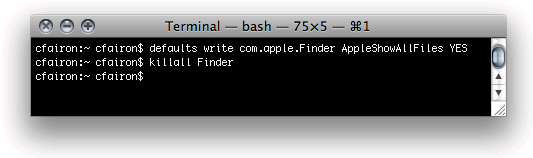
\includegraphics[width=12cm]{resources/img/fig-mac6.png}
%\caption{Restarting the Finder\label{fig-mac6}}
%\end{center}
%\end{figure}

%\bigskip
%\noindent To get back to the original configuration, type: 

%\bigskip
%\verb+defaults write com.apple.Finder AppleShowAllFiles OFF+


\section{First use}
\label{section-first-use}
If you work on Windows, the program will ask you to choose a
\index{Directory!personal working} personal working  directory, which you can
change later in "Info>Preferences...>Directories". To create a directory, click
on the icon showing a file (see
figure~\ref{fig-creation-personal-directory}).

\bigskip
\noindent If you are using Linux or MacOS, the program will automatically create a
personal working directory called \verb+/unitex+ in your \verb+$HOME+ directory.

\bigskip
\noindent The personal working directory, or user's directory, allows
you to save your personal Unitex data. For each language that you will be using, the
program will copy the root directory of that language to your working
directory, except the dictionaries. You can then modify your copy of the
files without risking to damage the system files stored in the
Unitex system directory.\index{Directory!Unitex system}

\begin{figure}[!ht]
\begin{center}
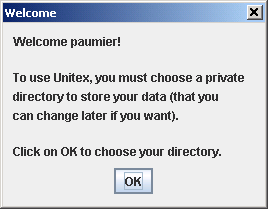
\includegraphics[width=6.3cm]{resources/img/fig1-1.png}
\caption{First use under Windows}
\end{center}
\end{figure}

\begin{figure}[!ht]
\begin{center}
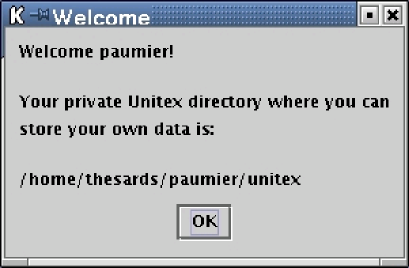
\includegraphics[width=7cm]{resources/img/fig1-2.png}
\caption{First use under Linux}
\end{center}
\end{figure}

\begin{figure}[!ht]
\begin{center}
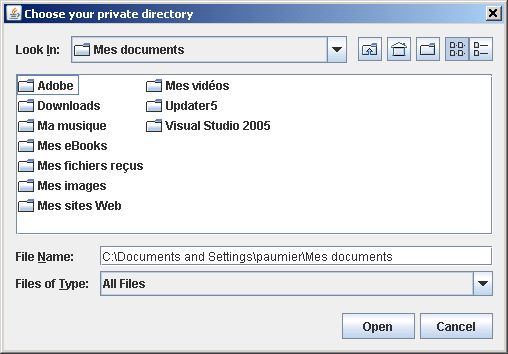
\includegraphics[width=13cm]{resources/img/fig1-3.png}
\caption{Creating the personal working
directory\label{fig-creation-personal-directory}}
\end{center}
\end{figure}



\section{Adding new languages}
\index{Adding languages}

\bigskip
\noindent There are two different ways to add languages. If you want to add 
a language that is to be accessible by all  users, you have to copy the 
corresponding directory to the Unitex system directory,\index{Directory!Unitex system} for which 
you will need to have the access rights  (this might mean that you need to 
ask your system administrator to do it). On the other hand, if you are the only user working
with the language, you can also copy the directory to your working 
directory.\index{Directory!personal working}
You can work with this language without it being shown to other users.


\section{Uninstalling Unitex}
No matter which operating system you are working with, it is sufficient to delete 
the Unitex system directory to completely delete all the program files. Under
Windows you may have to delete the shortcut to \verb+Unitex.jar+ \index{File!\verbc{Unitex.jar}} 
if you have created one on your desktop. The same has to be done on Linux, if you have 
created an alias.


\section{Unitex for developpers}
\label{section-unitex-developpers}
If you are a programmer, you may be interested in linking your code with Unitex
C++ sources. To facilitate such operation, you can compile Unitex as a
dynamic library that contains all Unitex functions, except \verb+main+s, of
course. Under Linux/MacOS, type:

\bigskip
\verb+make LIBRARY=yes+

\bigskip
\noindent and you will obtain a library named \verb+libunitex.so+. If you want
to produce a Windows DLL named \verb+unitex.dll+, use the following commands:

\bigskip
Windows: \verb+make SYSTEM=windows LIBRARY=yes+

Cross-compiling with mingw32: \verb+make SYSTEM=mingw32 LIBRARY=yes+

\bigskip
\noindent In all cases, you will also obtain a program named
\verb+Test_lib+(\verb+.exe+). If everything worked fine, this program should 
display the following:

\begin{verbatim}
Expression converted.
Reg2Grf exit code: 0

#Unigraph
SIZE 1313 950
FONT Times New Roman:  12
OFONT Times New Roman:B 12
BCOLOR 16777215
FCOLOR 0
ACOLOR 12632256
SCOLOR 16711680
CCOLOR 255
DBOXES y
DFRAME y
DDATE y
DFILE y
DDIR y
DRIG n
DRST n
FITS 100
PORIENT L
#
7
"<E>" 100 100 1 5
"" 100 100 0
"a" 100 100 1 6
"b" 100 100 1 4
"c" 100 100 1 6
"<E>" 100 100 2 2 3
"<E>" 100 100 1 1
\end{verbatim}

\chapter{Loading a text}
\label{chap-text}

One of the main functionalities of Unitex is to search a text for expressions.
To do that, texts have to undergo a set of preprocessing steps that  normalize
non-ambiguous forms and split the text  in sentences. Once these operations are
performed, the electronic dictionaries are applied to the texts. Then one  can
search more effectively in the texts by using  grammars.

\bigskip
\noindent This chapter describes the different steps for text preprocessing.


\section{Selecting a language}
\index{Selecting a language}\index{Language selection}
When starting Unitex, the program asks you to choose the language in which you
want to work (see figure~\ref{fig-language-selection}). The languages
displayed are the ones that are present in the \verb+Unitex+ system directory and those that
are  installed in your personal working directory. If you use a language for the
first time, Unitex copies the system directory for this language to your personal
directory, except for the dictionaries in order to save disk space.

\bigskip
\noindent WARNING: If
you already have a personal directory for a given language, Unitex won't try to
copy system data into it. So, if an update has modified a resource file other
than a dictionary, you will have to copy by yourself this file, or to delete your
personal directory for this language, and let Unitex rebuild it properly.

\bigskip
\noindent 
Choosing the language allows Unitex to find certain files, for example the
alphabet file. \index{File!alphabet} You can change the language at any time by
choosing "Change Language..." in the "Text" menu. If you change the language, the
program will close all windows related to the current text, if there are any. The
active language is indicated in the title bar of the graphical interface.

\begin{figure}[!h]
\begin{center}
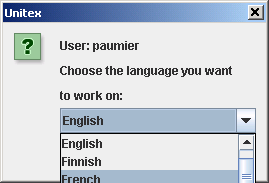
\includegraphics[width=6.2cm]{resources/img/fig2-1.png}
\caption{\label{fig-language-selection}Language selection when starting
Unitex}
\end{center}
\end{figure}


\section{Text formats}
\label{section-conversion-texte-unicode}
\index{Text!formats}
\index{Corpus|see{Text}}
\index{Unicode}
Unitex works with Unicode texts. Unicode is a standard that describes a universal
character code. Each character is given a unique number, which allows for
representing texts without having to take into account  the proprietary codes on
different machines and/or operating systems. Unitex uses a two-byte
representation of the Unicode 3.0 standard, called Unicode Little-Endian (for
more details, see \cite{UNICODE}).

\bigskip
\index{File!transcoding}
\noindent Texts that come with Unitex are already in Unicode format. If you try
to open a text that is not in Unicode, the program proposes to convert it
(see figure~\ref{auto-transcoding}).
This conversion is based on the current language: if you are working in French,
Unitex proposes to convert your text\,\footnote{Unitex also proposes to
automatically convert graphs and dictionaries that are not in Unicode
Little-Endian.} assuming that it is coded using a French code page. By default,
Unitex proposes to either replace the original text or to rename the original
file by inserting \verb$.old$ at the beginning of  its extension. For example, if
one has an ASCII file named \verb$biniou.txt$, the conversion process will create
a copy of this ASCII file named \verb$biniou.old.txt$, and will replace the
contents of \verb$biniou.txt$ with its equivalent in Unicode.


\begin{figure}[!h]
\begin{center}
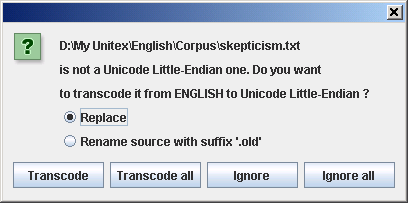
\includegraphics[width=10cm]{resources/img/fig2-2.png}
\caption{\label{auto-transcoding}Automatic conversion of a non-Unicode text}
\end{center}
\end{figure}

\noindent If the encoding suggested by default is not correct  or if you want to
rename the file differently than with the suffix \verb$.old$, you must use the "More options..." 
button. This allows you to choose source and
target encodings of the documents to be converted (see figure~\ref{transcoding}). By default,
the selected source encoding is that which corresponds to the current language
and the destination encoding is Unicode Little-Endian. You can modify these choices by selecting
any source and target encodings. Thus, if you wish, you can convert your data
into other encodings, as for example UTF-8 in order for instance to create web pages. The button
"Add Files" enables you to select the files to be converted. The button "Remove Files" makes it
possible to remove a list of files erroneously selected. The button "Transcode" will start the
conversion of all the selected files. If an error occurs with a file is
processed (for example, a file which is already in Unicode), the 
conversion continues with the next file.


\begin{figure}[!h]
\begin{center}
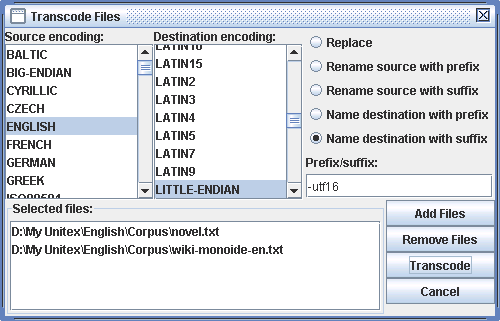
\includegraphics[width=12cm]{resources/img/fig2-3.png}
\caption{\label{transcoding}Transcoding files}
\end{center}
\end{figure}

\noindent To obtain a text in the right format, you can also use a text
processor like the free software from OpenOffice.org  (\cite{OpenOffice}) or Microsoft Word, and
save your document with the format "Unicode text".
In OpenOffice Writer, you have to choose the "Coded Text (*.txt)" format and then
select the "Unicode" encoding in the configuration window as shown on figure
\ref{OfficeWriter}.

\begin{figure}[!h]
\begin{center}
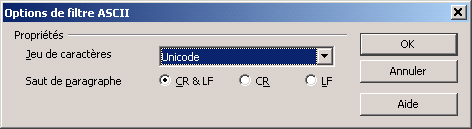
\includegraphics[width=12.5cm]{resources/img/fig2-4.png}
\caption{\label{OfficeWriter}Saving in Unicode with OpenOffice Writer}
\end{center}
\end{figure}

\noindent By default, the encoding proposed on a PC is always Unicode
Little-Endian. The texts thus obtained do not contain any formatting information anymore (fonts,
colors , etc.) and are ready to be used with Unitex.

\bigskip
\noindent 
You can change the default encoding to UTF16LE, UTF16BE or UTF8 in the 'Encoding' tab via the Preference  command in the Info menu. This encoding is valid for the current language only.

\begin{figure}[!h]
\begin{center}
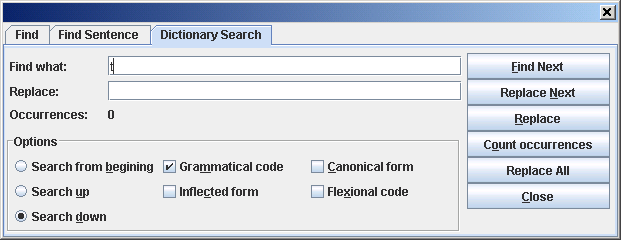
\includegraphics[width=10cm]{resources/img/fig2-5.png}
\caption{\label{OfficeWriter}Setting the default encoding for current language}
\end{center}
\end{figure}

\section{Editing text files}
For small texts, you also have the possibility of using the text editor integrated into Unitex,
accessible via the "Open..." command in the "File Edition" menu".
\index{Integrated text editor} This editor offers search and replace
functionalities  for the texts and dictionaries handled by Unitex. To use it,
click on the "Find" icon. You will then see a window  divided into three parts.
The "Find" part corresponds to the usual search operations. If you open a text
split into sentences, you can base your search on sentence numbers 
in the "Find Sentence" part. Lastly, the "Search Dictionary" part,
visible in figure~\ref{dictionary-search}, enables you to carry out operations
concerning the electronic dictionaries. In particular, you can   search by
specifying if it concerns  inflected forms, lemmas, grammatical and semantic
and/or inflectional codes. Thus, if you want to search for all the verbs which
have the  semantic feature \verb$t$, which indicates
transitivity, you just have to search for  \verb$t$ by clicking on "Grammatical
code". You will get the matching entries without confusion  with all the other
occurrences of the letter \verb$t$.


\begin{figure}[!h]
\begin{center}
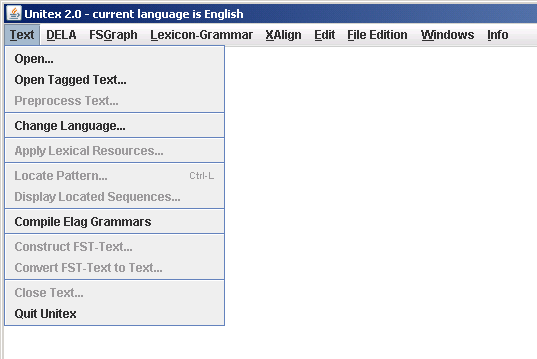
\includegraphics[width=15cm]{resources/img/fig2-6.png}
\caption{Searching an electronic dictionary for the semantic feature \texttt{t}\label{dictionary-search}}
\end{center}
\end{figure}


\section{Opening a text}
%Unitex deals with two types of text files. \index{File!text}
%The files with the extension \verb+.snt+ are text files preprocessed by Unitex
%which are ready to be manipulated by the different system functions. The files
%ending with \verb+.txt+ are raw files.
%To use a text, open the \verb+.txt+ file by clicking on "Open..." in the "Text"
%menu. Choose the file type "Raw Unicode Texts" and select your text.

Unitex deals with several types of documents. \index{File!text}
The files with the extension \verb+.snt+ are text files preprocessed by Unitex 
which are ready to be manipulated by the different system functions. 
You can also load raw files ending with \verb+.txt+, or XML and HTML files. 
To open any of these files, click on "Open..." in the
"Text" menu. You can there choose the file type ("Raw Unicode Texts", "XML files", "HTML files", "Unitex Texts").
If you open XML or HTML files, foo.xml for example, it will be preprocessed in order to remove non textual content. This will produce a foo.xml.txt file containing only the textual content of the original file. The resulting \verb+.txt+ file will be processed to produce a \verb+.snt+ file


\begin{figure}[!h]
\begin{center}
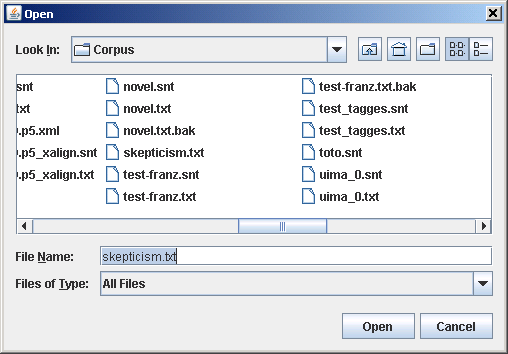
\includegraphics[width=14cm]{resources/img/fig2-7.png}
\caption{Text Menu}
\end{center}
\end{figure}

\begin{figure}[!h]
\begin{center}
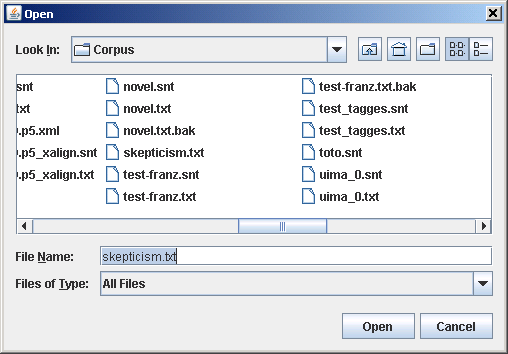
\includegraphics[width=13cm]{resources/img/fig2-8.png}
\caption{Opening a Unicode text}
\end{center}
\end{figure}

 

\section{Preprocessing a text}
\index{Text!preprocessing}
After a text is selected, Unitex offers to preprocess it. Text preprocessing
consists of performing the following operations: normalization of separators,
splitting into sentences, normalization of non-ambiguous forms, tokenization and 
application of dictionaries. If you choose not to preprocess the text, it 
will nevertheless be normalized and tokenized, since
these operations are necessary for all further Unitex operations. It is always
possible to carry out the preprocessing later by clicking on "Preprocess Text..."
in the "Text" menu. 

\begin{figure}[!h]
\begin{center}
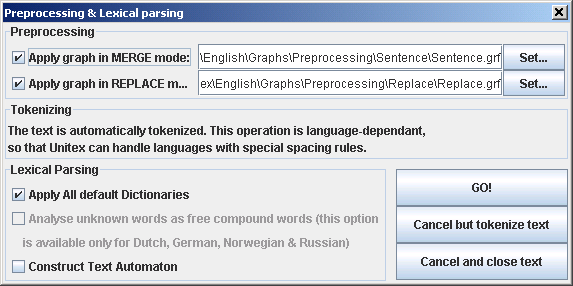
\includegraphics[width=15cm]{resources/img/fig2-9.png}
\caption{Preprocessing Window\label{fig-preprocessing-frame}}
\end{center}
\end{figure}

\bigskip
\noindent 
If you choose to preprocess the text, Unitex proposes to parameterize it
as in the window shown in figure~\ref{fig-preprocessing-frame}.
The option "Apply FST2 in MERGE mode" is used to split the text into sentences.
The option "Apply FST2 in REPLACE mode" is used to make replacements in the text,
especially for the normalization of non-ambiguous forms. With the option "Apply
All default Dictionaries" you can apply dictionaries in the DELA format
(Dictionnaires Electroniques du LADL).\index{DELA} The option "Analyze unknown
words as free compound words" is used in Norwegian for correctly analyzing
compound words  constructed via concatenation of simple forms.  Finally, the
option "Construct Text Automaton" is used to build the text automaton. This
option is deactivated by default, because it consumes a large amount of memory
and disk space if the text is too large. The construction of the text automaton
is described in chapter~\ref{chap-text-automaton}.

\bigskip
\noindent NOTE: If you click on "Cancel but tokenize text", the program will
carry out the normalization of separators and split the text into tokens. Click
on "Cancel and close text" to cancel the operation.

\subsection{Normalization of separators}
\index{Normalization!of separators}\index{Separators!word}\index{Word separators}\index{Text!normalization}
The standard separators are the space, the tab and the newline characters. There
can be several separators following each other, but since this isn't useful for
linguistic analyses, separators are normalized according to the following rules:

\begin{itemize}
  \item a sequence of separators that contains at least one newline is replaced by a single newline
  
  \item all other sequences of separators are replaced by a single space.
\end{itemize}

\bigskip
\noindent 
The distinction between space and newline is maintained at this point because the
presence of newlines may have an effect on the process of splitting the text into
sentences. The result of the normalization of a text named  \verb+my_text.txt+ is
a file in the same directory as the \verb+.txt+ file and is named
\verb+my_text.snt+. \index{File!\verb+.snt+}

\bigskip
\noindent NOTE: When the text is preprocessed using the graphical interface, a
directory named

% do not remove this line jump 
\noindent \verb+my_text_snt+ is created immediately after normalization.
This directory, called text directory,  \index{Directory!text}
\index{Text!directory} contains all the data associated with this text.



\subsection{Splitting into sentences}
\label{section-sentence-splitting}
\index{Splitting!into sentences}\index{Text!splitting into sentences}
\index{Grammars!splitting into sentences}
Splitting texts into sentences is an important preprocessing step since  this
helps in determining the units for linguistic processing. The splitting is used
by the text automaton construction program. In contrast to what one might think,
detecting sentence boundaries is not a trivial problem. Consider the following
text:

\bigskip
\textit{The family has urgently called Dr. Martin.}

\bigskip \noindent The full stop that follows \textit{Dr} is followed by a word
beginning with a capital letter. Thus it may be considered as the end of the
sentence, which would be wrong. To avoid the kind of problems caused by the
ambiguous use of punctuation, grammars are used to  describe the different
contexts for the end of a sentence.
Figure~\ref{fig-example-sentence-splitting} shows an example grammar for
sentence splitting (for French sentences).

\bigskip
\noindent When a path of the grammar recognizes a sequence in the text and when
this path produces the sentence delimiter symbol \verb+{S}+
\index{\verb+{S}+}\index{Sentence delimiter}, this symbol is inserted into the
text.

\bigskip
\noindent The path shown at the top of
figure~\ref{fig-example-sentence-splitting} recognizes the sequence consisting
of a question mark and a word beginning with a capital letter and inserts the 
symbol \verb+{S}+ between the question mark and
the following word. The following text:

\bigskip
\textit{What time is it? Eight o' clock.}

\bigskip
\noindent will be converted to:

\bigskip
\textit{What time is it ?\{S\} Eight o' clock.}

\bigskip
\noindent A  grammar for end-of-sentence detection may use the following
special symbols, or meta-symbols:

\index{\verb+<E>+}\index{Epsilon|see{<E>}}
\index{\verb+<MOT>+}\index{\verb+<MIN>+}\index{\verb+<MAJ>+}\index{\verb+<PRE>+}\index{\verb+<NB>+}
\index{\verb+<PNC>+}\index{\verb+<^>+}\index{\verb+#+}\index{Meta-symbols}
\begin{itemize}
  \item <E> : empty word, or epsilon. Recognizes the empty sequence;
  \item <MOT> : recognizes any sequence of letters;
  \item <MIN> : recognizes any sequence of letters in lower case;
  \item <MAJ> : recognizes any sequence of letters in upper case;
  \item <PRE> : recognizes any sequence of letters that begins with an upper case letter;
  \item <NB> : recognizes any sequence of digits (1234 is recognized but not 1
  234); \item <PNC> : recognizes the punctuation symbols \verb+ ; , ! ? :+ and the
  inverted exclamation points and question marks in Spanish and some Asian
  punctuation letters; \item <\verb+^+> : recognizes a newline; \item \verb+#+ :
  prohibits the presence of a space.
\end{itemize}

\begin{figure}[!h]
\begin{center}
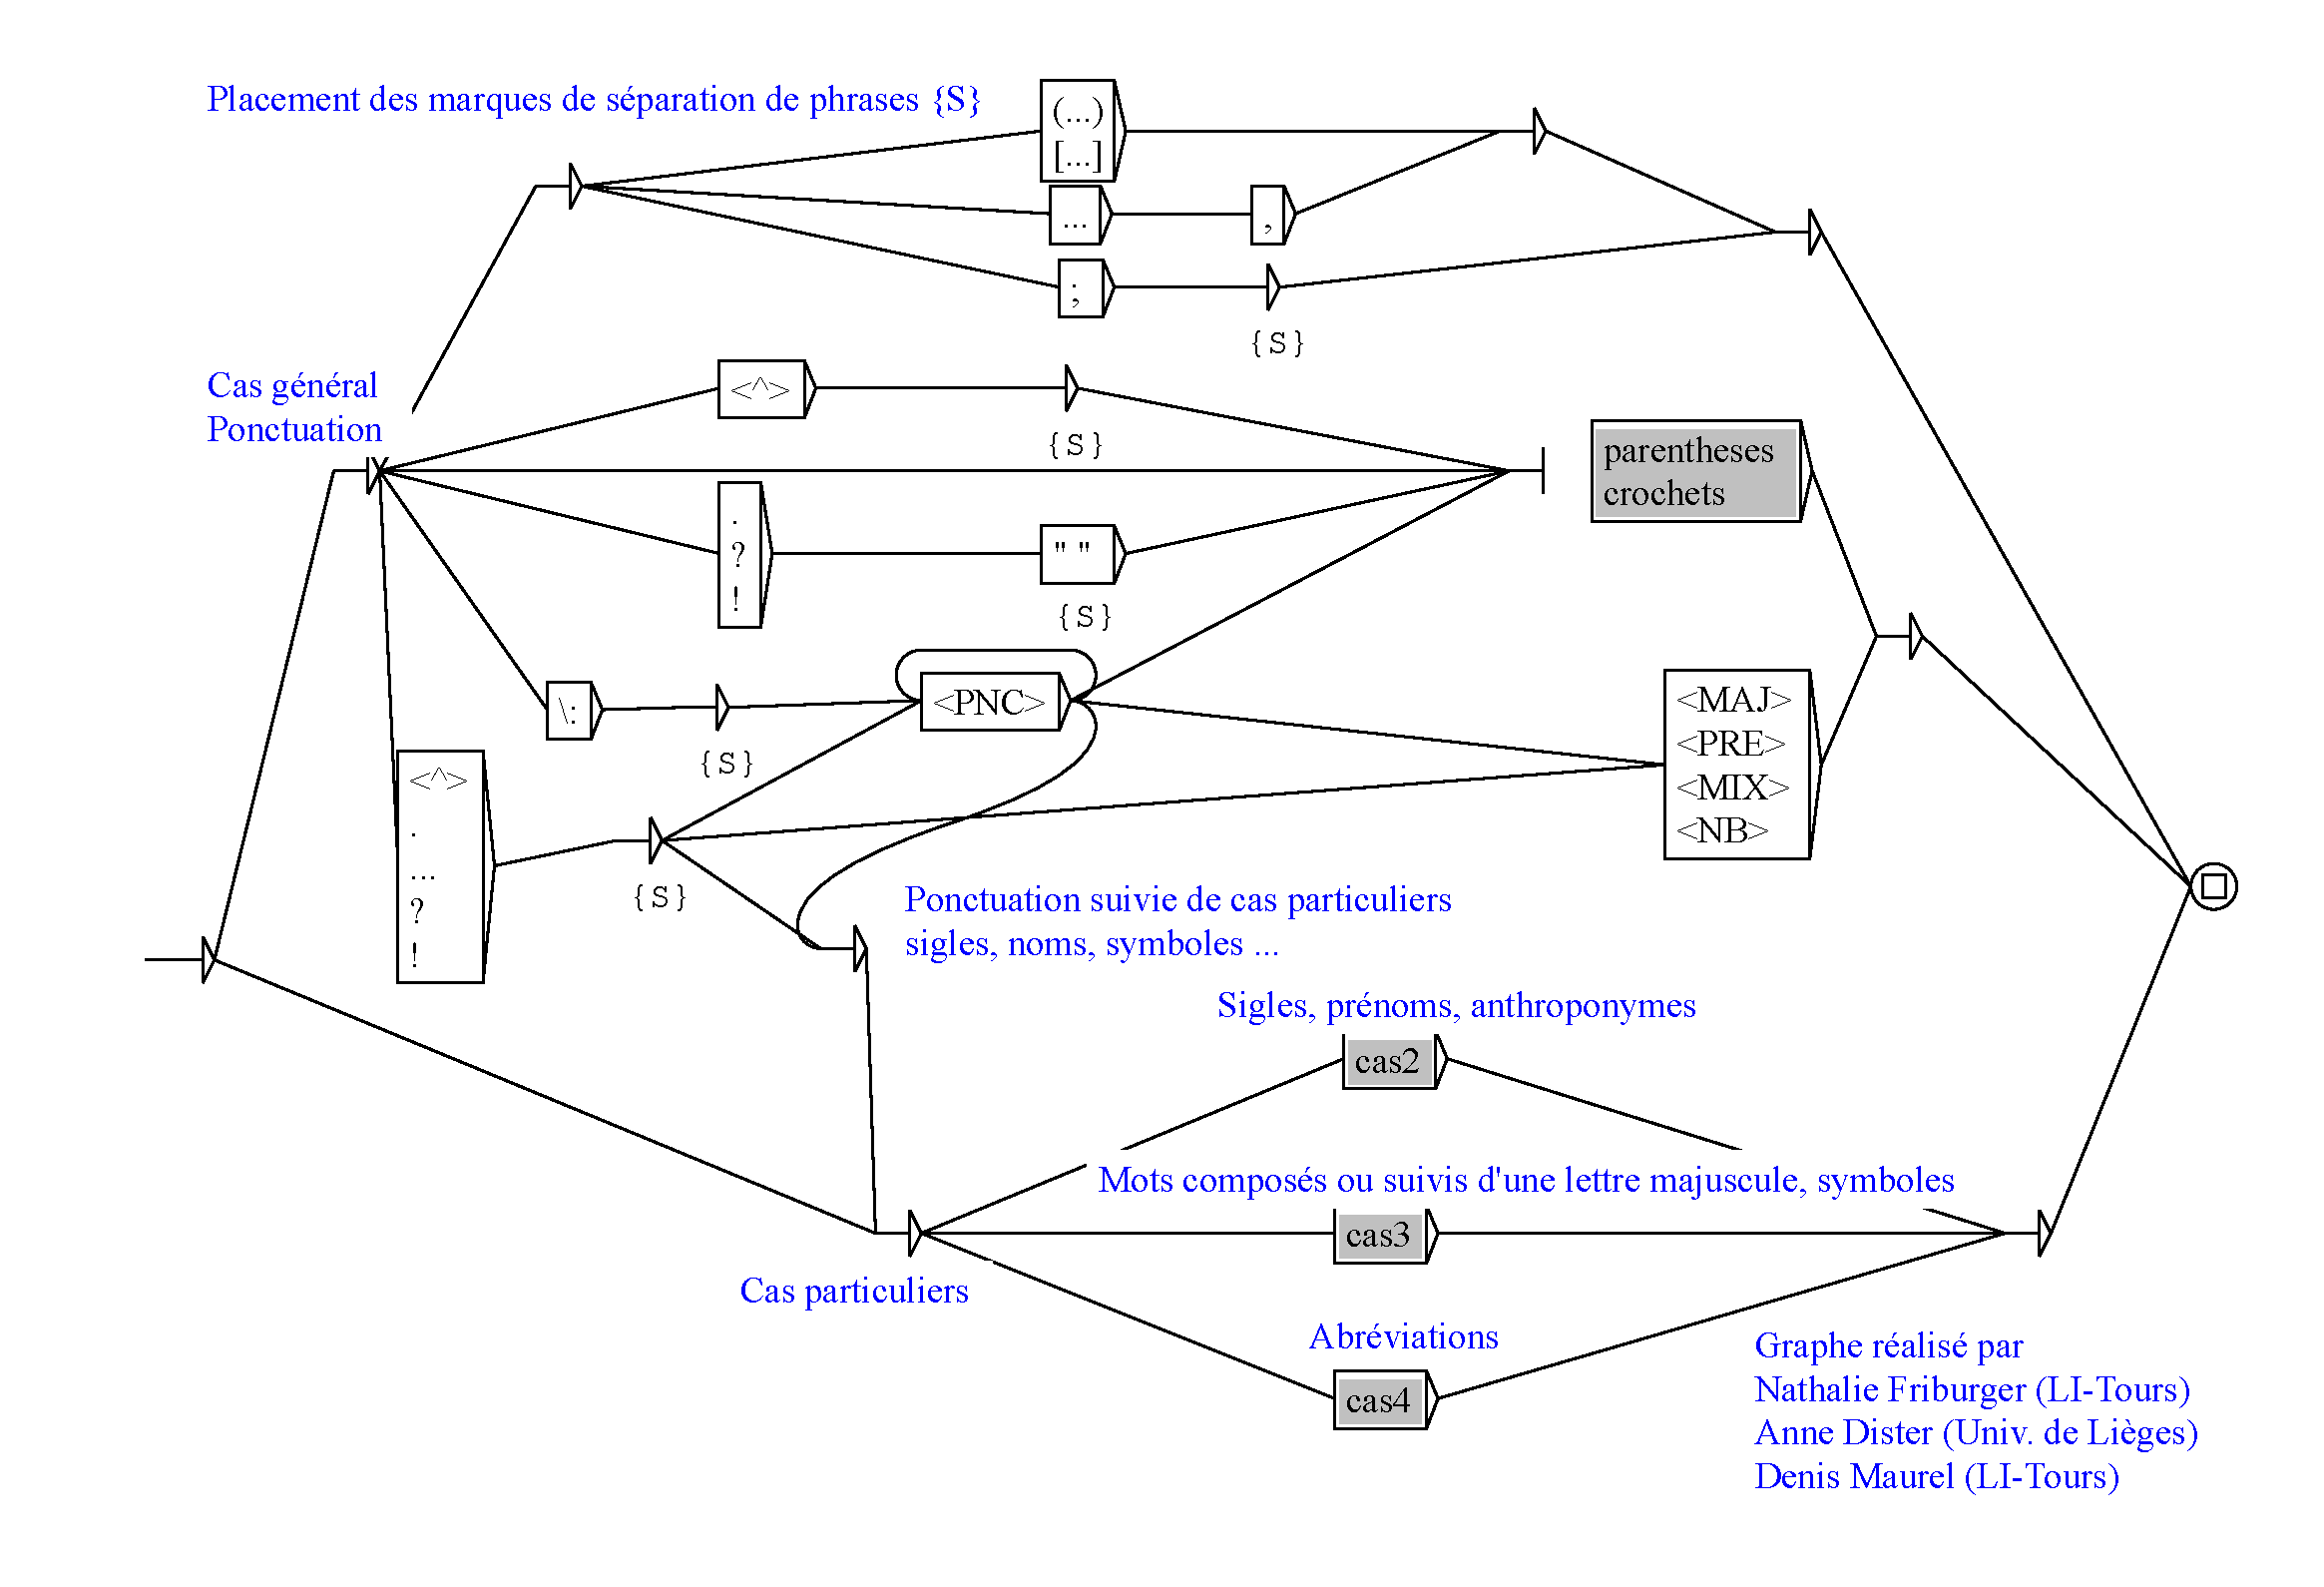
\includegraphics[width=15cm]{resources/img/fig2-10.pdf}
\caption{Sentence splitting grammar for
French\label{fig-example-sentence-splitting}}
\end{center}
\end{figure}

\bigskip
\noindent By default, the space is optional between two boxes. If you want to prohibit the
presence of the space you have to use the special character  \verb+#+. At the
opposite, if you want to force the presence of the space, you must use the
sequence \verb+" "+. Lower and upper case letters are defined by an alphabet
file\index{File!alphabet} (see chapter~\ref{chap-file-formats}). For
more details on grammars, see chapter~\ref{chap-grammars}.\index{Alphabet}
For more information about sentence boundary detection, see
\cite{ameliorer-decoupage-en-phrases}. The grammar used here is named
\verb+Sentence.fst2+ and can be found in the following directory:
\index{File!\verb+Sentence.fst2+}

\bigskip
\verb+/(user home directory)/(language)/Graphs/Preprocessing/Sentence+

\bigskip
\noindent This grammar is applied to a text with the \verb+Fst2Txt+ program
\index{\verb+Fst2Txt+}\index{External programs!\verb+Fst2Txt+} in
MERGE mode.\index{MERGE} This has the effect that the output produced
by the grammar, in this case the symbol \verb+{S}+, is inserted into
the text. This program takes a \verb+.snt+ file and modifies it.


\subsection{Normalization of non-ambiguous forms}
\index{Normalization!of non-ambiguous forms}
\index{Grammars!normalization!of non-ambiguous forms}

Certain forms present in texts can be normalized (for example, the English
sequence "\textit{I'm}" is equivalent to "\textit{I am}"). You may want to
replace these forms according to your own needs. However, you have to be careful
that the  forms normalized  are unambiguous or that the removal of ambiguity has
no undesirable consequences.

\bigskip
\noindent For instance, if you want to normalize "\textit{O'clock}" to "\textit{on the
clock}", it would be a bad idea to replace "\textit{O'}" by "\textit{on the }",
because a sentence like:

\bigskip
\textit{John O'Connor said: "it's 8 O'clock"}

\bigskip
\noindent would be replaced by the following incorrect sentence:

\bigskip
\textit{John on the Connor said: "it's 8 on the clock"}

\bigskip
\noindent Thus, one needs to be very careful when using the
normalization grammar. One needs to pay attention to spaces as well. 
For example, if one replaces "'re" by "are", the sentence:

\bigskip
\textit{You're stronger than him.}

\bigskip
\noindent will be replaced by:

\bigskip
\textit{Youare stronger than him.}

\bigskip
\noindent To avoid this problem, one should explicitly insert a space,
\textit{i.e.} replace "\textit{'re}" by "\textit{ are}".

\bigskip
\noindent The accepted symbols for the normalization grammar are the same as the ones
allowed for the sentence splitting grammar. The normalization grammar is called
\verb+Replace.fst2+ and can be found in the following directory:

\bigskip \verb+/(home directory)/(active language)/Graphs/Preprocessing/Replace+

\bigskip
\noindent As in the case of sentence splitting, this grammar is applied using the
\verb+Fst2Txt+ \index{External programs!\verb+Fst2Txt+}\index{\verb+Fst2Txt+}
program, but in REPLACE mode, which means that input sequences recognized by the
grammar are replaced by the output sequences that are produced.
Figure~\ref{fig-normalization-grammar} shows a grammar that
normalizes verbal contractions in English.

\begin{figure}[!p]
\begin{center}
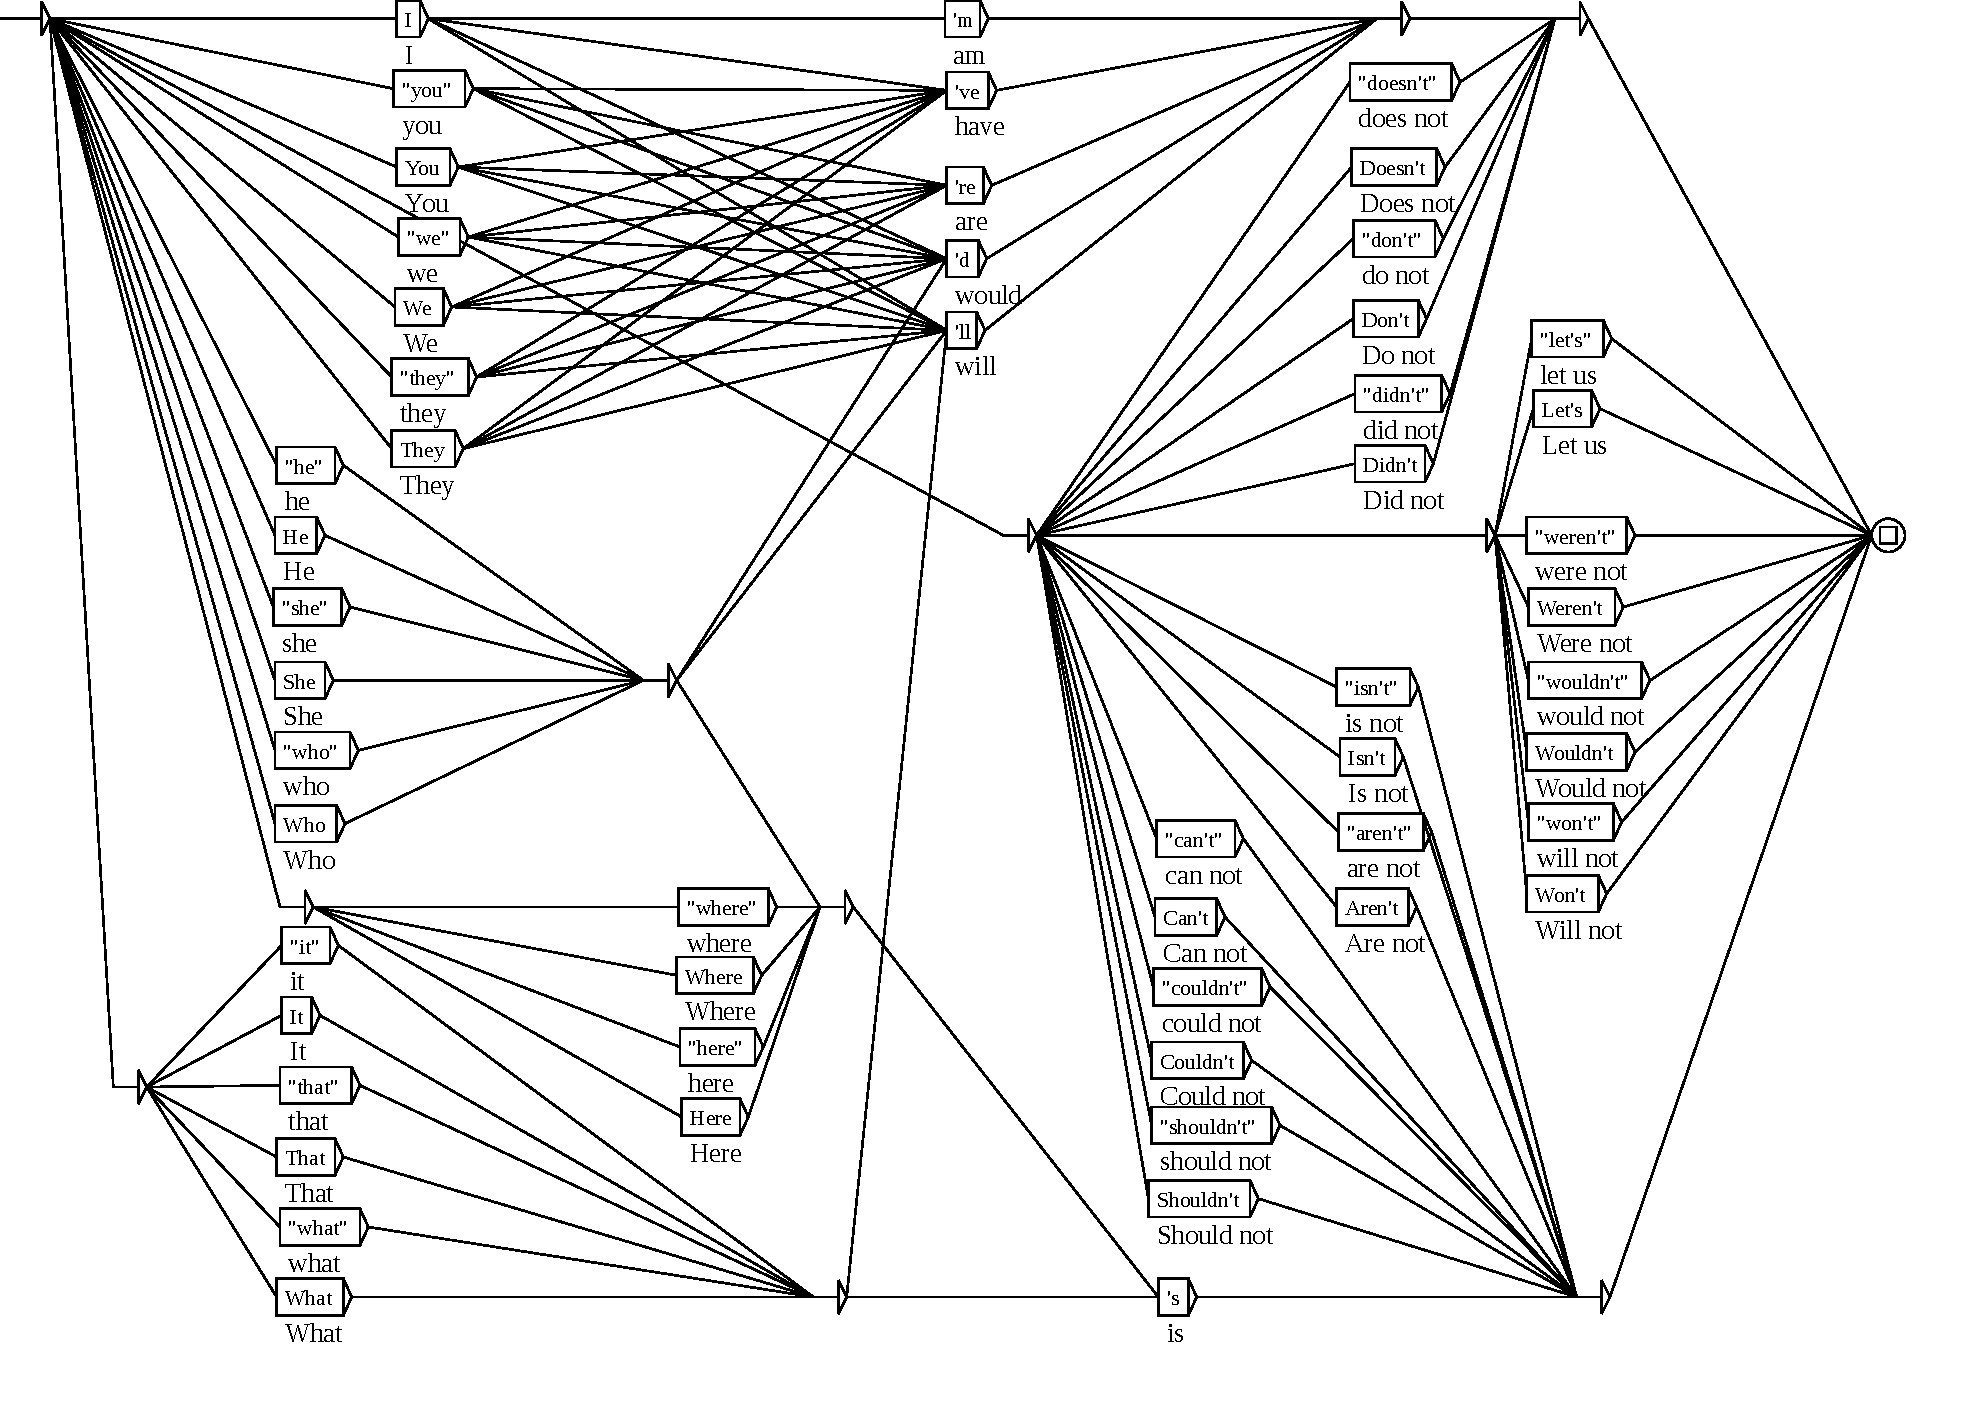
\includegraphics[height=17cm,angle=90]{resources/img/fig2-11.pdf}
\caption{Normalization of English verbal
contractions\label{fig-normalization-grammar}}
\end{center}
\end{figure}



\subsection{Splitting a text into tokens}
\index{Text!tokenization}
\index{Text!splitting into tokens}
\index{Splitting!into tokens}
\index{Token}
\index{Tokenization}
\label{tokenization}
Some languages, in particular Asian languages, use separators that are different
from the ones used in  western languages. Spaces can be forbidden, optional, or
mandatory. In order to better cope with these particularities,  Unitex splits
texts in a language dependent way. Thus, languages like English are treated as
follows:

\bigskip
\noindent A token can be:
\begin{itemize}
  \item the sentence delimiter \verb+{S}+; \item the stop marker
  \verb+{STOP}+.\index{\verb${STOP}$} This token is a special one that can
  NEVER be matched in any way by a grammar. It can be used to bound elements
  in a corpus. For instance, if a corpus is made of news separated by
  \verb+{STOP}+, it will be impossible that a grammar matches a sequence that
  overlaps the end of a news and the beginning of the following news;
  \item a lexical tag \verb+{aujourd'hui,.ADV}+; \item a contiguous sequence of
  letters (the letters are defined in the language alphabet file);
  \index{File!alphabet}
  \item one (and only one) non-letter character, i.e. all characters not defined
  in the alphabet file of the current language; if it is a newline, it is replaced by
  a space.
\end{itemize}

\bigskip
\noindent For other languages, tokenization is done on a character by character
basis, except for the sentence delimiter \verb+{S}+, the \verb+{STOP}+ marker
and lexical tags. This simple tokenization is fundamental for the use of Unitex,
but limits the optimization of search operations for patterns.

\bigskip
\noindent Regardless of the tokenization mode, newlines in a text are
replaced by spaces. Tokenization is done by the \verb+Tokenize+\index{\verb+Tokenize+}
\index{External programs!\verb+Tokenize+} program. This program creates several
files that are saved in the text directory:
\begin{itemize}
  \item \verb+tokens.txt+ contains the list of tokens in the order in which they are found in the text;
  \index{File!\verb+tokens.txt+}
  \item \verb+text.cod+ contains an integer array; every
  integer corresponds to the index of a token in the file \verb+tokens.txt+;
  \index{File!\verb+text.cod+}
  \item \verb+tok_by_freq.txt+ contains the list of tokens sorted by frequency;
  \index{File!\verb+tok_by_freq.txt+}
  \item \verb+tok_by_alph.txt+ contains the list of tokens in alphabetical order;
  \index{File!\verb+tok_by_alph.txt+}
  \item \verb+stats.n+ contains some statistics about the text. \index{File!\verb+stats.n+}
\end{itemize}

\bigskip
\noindent Tokenizing the text:

\bigskip
\textit{A cat is a cat.}

\bigskip
\noindent returns the following list of tokens: \textit{A} SPACE \textit{cat is a .}

\bigskip
\noindent You will observe that tokenization is case sensitive (\textit{A} and
\textit{a} are two distinct tokens), and that each token is listed only once.
Numbering these tokens from 0 to 5, the text can be represented by a sequence of
numbers (integers) as described in the following table:

\bigskip
\begin{table}[h]
\begin{center}
\begin{tabular}{|p{2.8cm}||c|c|c|c|c|c|c|c|c|c|c|c|}
\hline
Token number               & 0 & 1 & 2 & 1 & 3 & 1 & 4 & 1 & 2 & 5
\\
\hline
Corresponding token & \textit{A} &   & \textit{cat} &   & \textit{is} &  & \textit{a}
& & \textit{cat} & \textit{.}
\\
\hline
\end{tabular}
\caption{Representation of the text \textit{A cat is a cat.}}
\end{center}
\end{table}

\bigskip
\noindent For more details, see chapter~\ref{chap-file-formats}.

\begin{figure}[!h]
\begin{center}
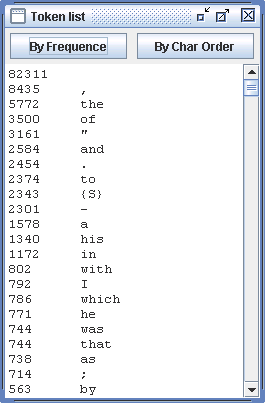
\includegraphics[height=10cm]{resources/img/fig2-12.png}
\caption{Tokens of an English text sorted by frequency}
\end{center}
\end{figure}



\subsection{Applying dictionaries}
\label{text-applying-dictionaries}
\index{Dictionaries!applying}
\index{Lexical!resources|see {Dictionaries}}
Applying dictionaries consists of building the subset of dictionaries  consisting
only of forms that are present in the text. Thus, the result of applying a
English dictionary to the text \textit{Igor's father in law is ill} produces a
dictionary of the following simple words:\index{Words!simple}

\bigskip
\begin{verbatim}
father,.N+Hum:s
father,.V:W:P1s:P2s:P1p:P2p:P3p
ill,.A
ill,.ADV
ill,.N:s
in,.A
in,.N:s
in,.PART
in,.PREP
is,be.V:P3s
is,i.N:p
law,.N:s
law,.V:W:P1s:P2s:P1p:P2p:P3p
s,.N:s
\end{verbatim}

\bigskip
\noindent as well as a dictionary of compound words consisting of a single
entry:\index{Words!compound}

\bigskip
\begin{verbatim}
father in law,.N+NPN+Hum+z1:s
\end{verbatim}

\bigskip
\noindent Since the sequence \textit{Igor} is neither a simple English word nor a part of a
compound word, it is treated as an unknown word. \index{Words!unknown} The
application of dictionaries is done through the program \verb+Dico+.
\index{\verb+Dico+}\index{External programs!\verb+Dico+} The three files produced
(\verb+dlf+ for simple words, \verb+dlc+ for compound words and \verb+err+ for
unknown words) are placed in the text directory. The \verb+dlf+ and \verb+dlc+
files are called text dictionaries.  \index{Dictionaries!text}
\index{File!\verb+dlf+}
\index{File!\verb+dlc+}\index{File!\verb+err+}

\bigskip
\noindent As soon as the dictionary look-up  is finished, Unitex displays the sorted lists
of simple, compound and unknown words found in a new window.
Figure~\ref{fig-Dico-application-results} shows the result for an
English text.

\begin{figure}[!ht]
\begin{center}
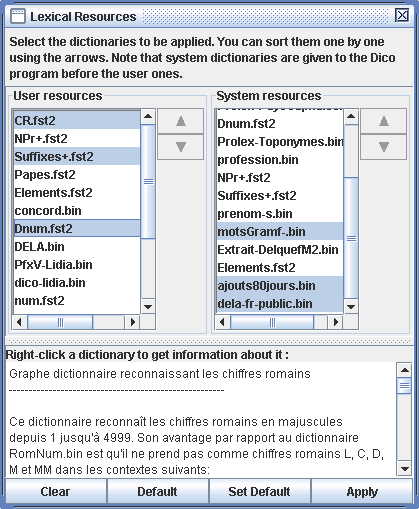
\includegraphics[width=12cm]{resources/img/fig2-13.png}
\caption{Result after applying dictionaries to an English text\label{fig-Dico-application-results}}
\end{center}
\end{figure}

\bigskip
\noindent It is also possible to apply dictionaries without preprocessing the text. In
order to do this, click on "Apply Lexical Resources..." in the "Text" menu.
Unitex then opens a window (see
figure~\ref{fig-Dico-configuration}) in which you can select
the list of dictionaries to apply.

\begin{figure}[!ht]
\begin{center}
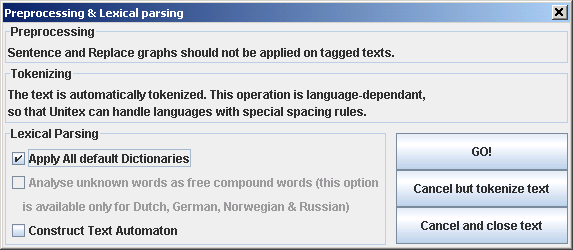
\includegraphics[width=10cm]{resources/img/fig2-14.png}
\caption{Parameterizing the application of dictionaries\label{fig-Dico-configuration}}
\end{center}
\end{figure}

\bigskip
\noindent The list "User resources" lists all dictionaries present in the
directory

% DO NOT REMOVE THIS LINE JUMP!
\noindent \verb+(current language)/Dela+ of the user. The dictionaries installed
in the system are listed in the scroll list  named "System resources". Use the
<Ctrl+click> combination to select several dictionaries. System dictionaries
will be applied prior to user dictionaries. Within the system or user list, you
can fix the order of dictionaries using the up and down arrows, as shown on
figure \ref{fig-Dico-configuration}. The button "Set
Default" allows you to define the current selection of dictionaries  as the
default. This default selection will then be used during preprocessing if you
activate the option "Apply All default Dictionaries".\index{Dictionaries!default
selection} If you right-click on a dictionary name, the associated documentation,
if any, will be displayed in the lower frame of the window.


\subsection{Analysis of compound words in Dutch, German, Norwegian and Russian}
\index{Norwegian!free compound words}\index{German!free compound words}\index{Dutch!free compound words}
\index{Russian!free compound words}
\index{Analysis of free compound words!in Germanic languages}\index{Words!compound!in Germanic languages}
\index{Analysis of free compound words!in Russian}\index{Words!compound!in Russian}
\label{section-Norwegian-compound-words}
In certain languages like Norwegian, German and others, it is possible to form
new compound words by concatenating  together other words. For example, the word
\textit{aftenblad} meaning \textit{evening journal} is obtained by combining the
words \textit{aften} (\textit{evening}) et \textit{blad} (\textit{journal}). The
\verb+PolyLex+ program \index{\verb+PolyLex+}\index{External
programs!\verb+PolyLex+} parses the list of unknown words after the application
of dictionaries and tries to analyze each of these words as a compound word. If
a word has at least one analysis as a compound word,  it is removed from the
list of unknown words and the lines produced for this word are appended to the
simple word text dictionary.



\section{Opening a tagged text}
A tagged text is a text containing words with lexical tags enclosed in braces:

\bigskip
\textit{I do not like the \{square bracket,.N\} sign! \{S\}}

\bigskip
\noindent Such tags can be used to avoid ambiguities. In the previous example,
it will be impossible to match \textit{square bracket} as the combination of two
simple words.

\bigskip
\noindent However, the presence of these tags can alter the application of
preprocessing graphs. To avoid complications, you can use the "Open Tagged
Text..." command in the "Text" menu. With it, you can open a tagged text and skip
the application of preprocessing graphs, as shown on Figure
\ref{preprocess-tagged-text}.

\bigskip
\begin{figure}[!h]
\begin{center}
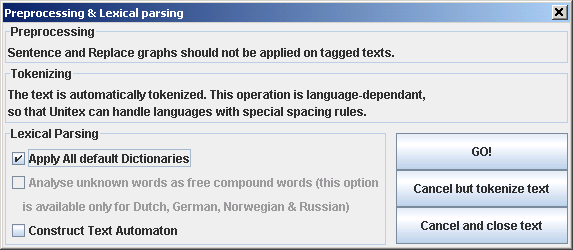
\includegraphics[width=14cm]{resources/img/fig2-15.png}
\caption{Preprocessing a tagged text\label{preprocess-tagged-text}}
\end{center}
\end{figure}

\chapter{Dictionaries}
\label{chap-dictionaries}

\section{The DELA dictionaries}
\index{DELA}\index{Dictionaries!format}\index{LADL}

The electronic dictionaries distributed with Unitex use the DELA syntax
(Dictionnaires Electroniques du LADL, LADL electronic dictionaries). This syntax
describes the simple and compound lexical entries \index{Lexical!entries} of a
language with their grammatical, semantic and inflectional information. We
distinguish two kinds of electronic dictionaries. The one that is used most often
is the  dictionary of inflected forms DELAF (DELA de formes Fl\'echies, DELA of
inflected forms) or DELACF (DELA de formes Compos\'ees Fl\'echies, DELA of
compound inflected forms) in the case of compound forms.\index{DELAF|(}
\index{DELACF}\index{Dictionaries!DELAF|(}\index{Dictionaries!DELACF}
The second type is a dictionary of non-inflected forms called DELAS (DELA de
formes simples, simple forms DELA) or DELAC (DELA de formes compos\'ees,
compound forms DELA).
\index{DELAS}\index{DELAC}\index{Dictionaries!DELAS}\index{Dictionaries!DELAC}

\bigskip
\noindent Unitex programs make no  distinction between simple and compound form
dictionaries. We will use the terms DELAF and DELAS to distinguish the
inflected and non-inflected dictionaries, no matter they contain simple word,
compound words or both. 

\subsection{The DELAF format}
\label{section-DELAF-format}
\subsubsection{Entry syntax}
An entry of a DELAF is a line of text terminated by a newline that conforms to
the following syntax:

\bigskip
\begin{verbatim}
apples,apple.N+conc:p/this is an example
\end{verbatim}

\bigskip
\noindent The different elements of this line are:

\bigskip
\begin{itemize}
  \item \verb+apples+ is the inflected form of the entry;\index{Form!inflected} it is mandatory;
  
  \bigskip \item \verb+apple+ is the canonical form (lemma) of the
  entry.\index{Lemma} \index{Form!canonical}For nouns and adjectives (in French), it is usually the
  masculine singular form; for verbs, it is the infinitive. This information may
  be left out as in the following example:
  
  \bigskip
  \verb$apple,.N+Conc:s$
  
  \bigskip This means that the canonical form is the same as the inflected form.
  The canonical form is separated from the inflected form by a
  comma.\index{\verb+,+}
  
  \bigskip \item \verb$N+Conc$ is the sequence of grammatical and semantic
  information. \index{Information!grammatical} \index{Information!semantic}In our
  example, \verb+N+ designates a noun, and \verb+Conc+ indicates that this noun
  designates a concrete object (see table~\ref{tab-semantic-codes}).
  
  Each entry must have at least one grammatical or semantic code, separated from
  the canonical form by a period. If there are more codes, these are separated by
  the \verb$+$\index{\verb$+$}\index{\verb+.+} character.
  
  \bigskip \item \verb+:p+ is an inflectional code which indicates that the noun
  is  plural.\index{Information!inflectional} Inflectional codes are used to
  describe gender, number, declension, and conjugation. This information is
  optional. An inflectional code is made up of one or more characters that
  represent one information each. Inflectional codes have to be separated by the
  : character, for instance in an entry like the following:
  
  \verb+hang,.V:W:P1s:P2s:P1p:P2p:P3p+
  
  The \verb+:+ character is interpreted in OR semantics. Thus,
  \verb+:W:P1s:P2s:P1p:P2p:P3p+ means "infinitive", or "1st person singular
  present", or "2nd person singular present", etc. (see
  table~\ref{tab-inflectional-codes}) Since each character
  represents one information, you must not use the same character
  more than once. In this way, encoding the past participle using the code \verb+:PP+ would be
  exactly equivalent to using \verb+:P+ alone;\index{\verb+:+}
  
  \bigskip \item \verb+/this is an example+ is a comment. Comments are optional
  and are introduced by the \verb+/+ character. These comments are left out when
  the dictionaries are compressed. \index{Comment!in a dictionary}
  \index{Dictionaries!comments in} \index{\verb+/+}
\end{itemize}

\bigskip
\noindent IMPORTANT REMARK: It is possible to use the full stop and the comma
within a dictionary entry. In order to do this they have to be escaped using the
\verb+\+ \index{\verb+\,+}\index{\verb+\.+}\index{\verb+\+} character:

\bigskip
\begin{verbatim}
1\,000,one thousand.NUMBER
United Nations,U\.N\..ACRONYM
\end{verbatim}


\bigskip
\noindent WARNING: Each character is taken into account within a dictionary
line. For example, if you insert spaces, they are considered to be a part of the
information. In the following line:

\begin{verbatim}
hath,have.V:P3s /old form of 'has'
\end{verbatim}

\bigskip \noindent The space that precedes the \verb+/+ character will be
considered to be part of a 4-character inflectional code.

\bigskip \noindent It is possible to insert comments into a DELAF or DELAS
dictionary by starting the line with a $/$ character. Example:

\bigskip
\begin{verbatim}
/ 'English' designates a pool spin
English,.N+z3:s
\end{verbatim}


\subsubsection{Compound words with spaces or dashes}

\index{Words!compound!with space or dash}\index{\verb+=+}\index{\verb+\=+}

Certain compound words like \textit{acorn-shell} can be written using spaces or
dashes. In order to avoid duplicating the entries, it is possible to use the
\verb+=+ character. At the time when the dictionary is compressed, the
\verb+Compress+ program \index{External
programs!\verb+Compress+}\index{\verb+Compress+} checks for each line if the
inflected or canonical form contains a non-escaped \verb+=+ character. If this is
the case, the program replaces this by two entries: one where the \verb+=+
character is replaced by a space, and one where it is replaced by a dash. Thus,
the following entry:

\bigskip \verb$acorn=shells,acorn=shell.N:p$

\bigskip
\noindent is replaced by the following entries:

\bigskip
\verb$acorn shells,acorn shell.N:p$

\verb$acorn-shells,acorn-shell.N:p$

\bigskip
\noindent NOTE: If you want to keep an entry that includes the \verb+=+
character, escape it using \verb+\+ as in the following example:

\bigskip \verb$E\=mc2,.FORMULA$

\bigskip
\noindent This replacement is done when the dictionary is compressed. In the compressed
dictionary, the escaped \verb+=+ characters are replaced by simple \verb+=+. As
such, if a dictionary containing the following lines is compressed:


\bigskip
\verb$E\=mc2,.FORMULA$

\bigskip
\verb$acorn=shell,.N:s$

\bigskip
\noindent and if the dictionary is applied to the following text:

\bigskip
\textit{Formulas like E=mc2 have nothing to do with acorn-shells.}

\bigskip \noindent you will get the following lines in the dictionary of compound
words of the text:


\begin{verbatim}
E=mc2,.FORMULA

acorn-shells,.N:p
\end{verbatim}


\subsubsection{Entry Factorization}

Several entries containing the same inflected and canonical forms can be
combined into a single one if they also share the same grammatical and semantic
codes. Among other things this allows us to combine identical conjugations for a verb:

\bigskip
\begin{verbatim}
bottle,.V:W:P1s:P2s:P1p:P2p:P3p
\end{verbatim}

\bigskip 
\noindent If the grammatical and semantic information differ, one has to create
distinct entries:

\bigskip
\begin{verbatim}
bottle,.N+Conc:s
bottle,.V:W:P1s:P2s:P1p:P2p:P3p
\end{verbatim}

\bigskip 
\noindent Some entries that have the same grammatical and semantic entries can
have different meanings, as it is the case for the French word \textit{po\^ele}
that describes a stove or a type of sheet in the masculine sense and a kitchen
instrument in the feminine sense. You can thus distinguish the entries in  this
case:

\bigskip
\noindent
\texttt{po\^ele,.N+z1:fs/ po\^ele \`a frire}

\noindent
\texttt{po\^ele,.N+z1:ms/ voile, linceul; appareil de chauffage}

\bigskip 
\noindent NOTE: In practice, this distinction has the only consequence that the
number of entries in the dictionary increases.

\bigskip 
\noindent For the different programs that make up Unitex these entries are equivalent to:

\bigskip
\noindent
\texttt{po\^ele,.N+z1:fs:ms}

\bigskip 
\noindent Whether this distinction is made is thus left to the  maintainers of  the dictionaries.

\index{DELAF|)}\index{Dictionaries!DELAF|)}

\subsection{The DELAS Format}
\label{section-DELAS-format}
\index{DELAS}\index{Dictionaries!DELAS}

The DELAS format is very similar to the one used in the DELAF. The only
difference is that there is only a canonical form followed by grammatical
and/or semantic codes. The canonical form is separated from the different codes
by a comma. There is an example: \index{\verb+,+}

\begin{verbatim}
horse,N4+Anl
\end{verbatim}

\noindent The first grammatical or semantic code will be interpreted by the
inflection program as the name of the grammar used to inflect the entry. The entry of the
example above indicates that the word \textit{horse} has to be inflected using
the grammar named \verb+N4+. It is possible to add inflectional codes to the
entries, but the nature of the inflection operation limits the usefulness of this
possibility. For more details see below in
section~\ref{section-automatic-inflection}.


\subsection{Dictionary Contents}
\index{Dictionaries!contents}\index{Dictionaries!codes used within}

The dictionaries provided with Unitex contain descriptions of simple and compound
words. These descriptions indicate the grammatical category of each entry,
optionally their inflectional codes, and various semantic information. The
following tables give an overview of some of the different codes used in the 
Unitex dictionaries. These codes are the same for almost all languages, though
some of them are special for certain languages (\textit{i.e.} code for neuter
nouns, etc.).

\begin{table}[!h]
\index{\verb+A+}\index{\verb+ADV+}\index{\verb+CONJC+}\index{\verb+CONJS+}\index{\verb+DET+}
\index{\verb+INTJ+}\index{\verb+N+}\index{\verb+PREP+}\index{\verb+PRO+}\index{\verb+V+}
\begin{center}
\begin{tabular}{|c|l|l|}
\hline
\textbf{Code} & \textbf{Description} & \textbf{Examples} \\
\hline
\verb+A+ & adjective & fabulous, broken-down \\
\hline
\verb+ADV+ & adverb & actually, years ago \\
\hline
\verb+CONJC+ & coordinating conjunction & but\\
\hline
\verb+CONJS+ & subordinating conjunction & because \\
\hline
\verb+DET+ & determiner & each \\
\hline
\verb+INTJ+ & interjection & eureka \\
\hline
\verb+N+ & noun & evidence, group theory \\
\hline
\verb+PREP+ & preposition & without \\
\hline
\verb+PRO+ & pronoun & you \\
\hline
\verb+V+ & verb & overeat, plug-and-play \\
\hline
\end{tabular}
\caption{Frequent grammatical codes\label{tab-grammatical-codes}}
\end{center}
\end{table}

\begin{table}[!h]
\index{\verb+z1+}\index{\verb+z2+}\index{\verb+z3+}\index{\verb+Abst+}\index{\verb+Anl+}\index{\verb+AnlColl+}
\index{\verb+Conc+}\index{\verb+ConcColl+}\index{\verb+Hum+}\index{\verb+HumColl+}\index{\verb+t+}\index{\verb+i+}
\index{\verb+en+}\index{\verb+se+}\index{\verb+ne+}
\begin{center}
\begin{tabular}{|c|l|l|}
\hline
\textbf{Code} & \textbf{Description} & \textbf{Example} \\
\hline
\verb+z1+ & general language & joke \\
\hline
\verb+z2+ & specialized language & floppy disk \\
\hline
\verb+z3+ & very specialized language & serialization \\
\hline
\verb+Abst+ & abstract & patricide \\
\hline
\verb+Anl+ & animal & horse \\
\hline
\verb+AnlColl+ & collective animal & flock \\
\hline
\verb+Conc+ & concrete & chair \\
\hline
\verb+ConcColl+ & collective concrete & rubble \\
\hline
\verb+Hum+ & human & teacher \\
\hline
\verb+HumColl+ & collective human & parliament \\
\hline
\verb+t+ & transitive verb & kill \\
\hline
\verb+i+ & intransitive verb & agree \\
\hline
\end{tabular}
\caption{Some semantic codes\label{tab-semantic-codes}}
\end{center}
\end{table}

\bigskip
\noindent NOTE: The  descriptions of tense in
table~\ref{tab-inflectional-codes} correspond to French.
Nontheless, the majority of these definitions can be found in other languages (infinitive, present, past participle, etc.).

\bigskip
\noindent In spite of a common base in the majority of languages, the dictionaries
contain encoding particularities that are specific for each language. Thus, as
inflectional codes vary a lot between different languages, they are not
described here. For a complete description of all codes used within a dictionary,
we recommend that you  contact the author of the dictionary directly.

\begin{table}[!h]
\index{\verb+m+}\index{\verb+f+}\index{\verb+n+}\index{\verb+s+}\index{\verb+p+}\index{\verb+1+}
\index{\verb+2+}\index{\verb+3+}\index{\verb+P+}\index{\verb+I+}\index{\verb+S+}\index{\verb+T+}
\index{\verb+Y+}\index{\verb+C+}\index{\verb+J+}\index{\verb+W+}\index{\verb+G+}\index{\verb+K+}\index{\verb+F+}
\begin{center}
\begin{tabular}{|c|l|}
\hline
\textbf{Code} & \textbf{Description} \\
\hline
\verb+m+ & masculine \\
\hline
\verb+f+ & feminin \\
\hline
\verb+n+ & neuter \\
\hline
\verb+s+ & singular \\
\hline
\verb+p+ & plural \\
\hline
\verb+1+, \verb+2+, \verb+3+ & 1st, 2nd, 3rd person\\
\hline
\verb+P+ & present indicative \\
\hline
\verb+I+ & imperfect indicative  \\
\hline
\verb+S+ & present subjunctive \\
\hline
\verb+T+ & imperfect subjunctive  \\
\hline
\verb+Y+ & present imperative \\
\hline
\verb+C+ & present conditional \\
\hline
\verb+J+ & simple past indicative \\
\hline
\verb+W+ & infinitive \\
\hline
\verb+G+ & present participle \\
\hline
\verb+K+ & past participle \\
\hline
\verb+F+ & future indicative \\
\hline
\end{tabular}
\caption{Common inflectional codes\label{tab-inflectional-codes}}
\end{center}
\end{table}

\bigskip
\noindent However, these codes are not exclusive. A user can introduce his own codes
and create his own dictionaries. For example, for educational purposes one could
use a marker "faux-ami" (\textit{false friend}) in a French dictionary:

\bigskip
\noindent
\texttt{blesser,.V+faux-ami/injure}

\noindent
\texttt{casque,.N+faux-ami/helmet}

\noindent
\texttt{journ\'ee,.N+faux-ami/day}


\bigskip
\noindent It is equally possible to use dictionaries to add extra information.
Thus, you can use the inflected form of an entry to describe an abbreviation and the
canonical form to provide the complete form:

\bigskip
\begin{verbatim}
DNA,DeoxyriboNucleic Acid.ACRONYM
LADL,Laboratoire d'Automatique Documentaire et Linguistique.ACRONYM
UN,United Nations.ACRONYM
\end{verbatim}


%%%%%%%%%%%%%%%%%%%%%%%%%%%%%%%%%%%%%%%%%%%%%%%%%%%
\section{Looking up a word in a dictionary}
\index{Dictionaries!lookup} \index{Looking up a word in a dictionary}
\label{section-dictionary-lookup}
You can look up a word in one or several dictionaries by two means : 

\begin{figure}[h!]
\begin{center}
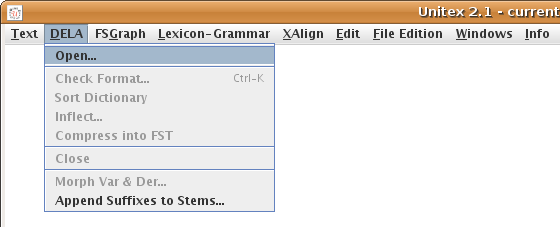
\includegraphics[width=13cm]{resources/img/fig3-1.png}
\caption{"DELA" Menu}
\end{center}
\end{figure}

\bigskip
\noindent
If you have opend a dictionary, the displayed window contains a field where you can enter a word to search. If the word appears in the dictionary, the Find Button will highlight the first entry that matches it. If there is several entries for this word, you can browse all matches by clicking on the two arrow buttons.

\begin{figure}[h!]
\begin{center}
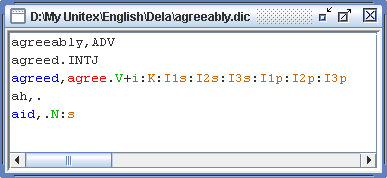
\includegraphics[width=7cm]{resources/img/fig3-2.png}
\caption{Looking up for a word in a dictionnary}
\end{center}
\end{figure}

\bigskip
\noindent
You can also look up a word in several dictionnaries by clicking on the Lookup button of the DELA menu. You can then select the dictionaries in which you want to look up the word you have entered.

\begin{figure}[h!]
\begin{center}
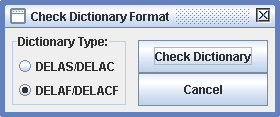
\includegraphics[width=7cm]{resources/img/fig3-3.png}
\caption{Looking up for a word in several dictionnaries}
\end{center}
\end{figure}

\bigskip
\noindent

%%%%%%%%%%%%%%%%%%
\section{Checking dictionary format}
\index{Dictionaries!checking} \index{Checking dictionary format}
When dictionaries become large, it becomes tiresome to check them by hand.
Unitex contains the program \verb+CheckDic+\index{External
programs!\verb+CheckDic+}\index{\verb+CheckDic+} that automatically checks the
format of DELAF and DELAS dictionaries.

\bigskip
\noindent This program verifies the syntax of the entries. For each malformed
entry the program outputs the line number, the content of the line and an error
message. Results are saved in the file
\verb+CHECK_DIC.TXT+\index{File!\verb+CHECK_DIC.TXT+} which is displayed when the
verification is finished. In addition to eventual error messages, the file also
contains the list of all characters used in the inflectional and canonical forms,
the list of grammatical and semantic codes, and the list of inflectional codes
that appear in the dictionary. The character list makes it possible to verify
that the characters used in the dictionary are consistent with those in the 
alphabet file of the language. Each character is followed by its value in hexadecimal
notation.\index{File!alphabet}

\bigskip
\noindent The code lists can be used to check that there are no typing errors 
in the codes of the dictionary.

\bigskip
\noindent The \verb+CheckDic+ program works with non-compressed dictionaries,
\textit{i.e.} the files in text format. The general convention is to use the
\verb+.dic+ extension for these dictionaries. In order to check the 
\index{File!\verb+.dic+} format of a
dictionary, you first open it by choosing "Open..." in the "DELA" menu.

\begin{figure}[h]
\begin{center}
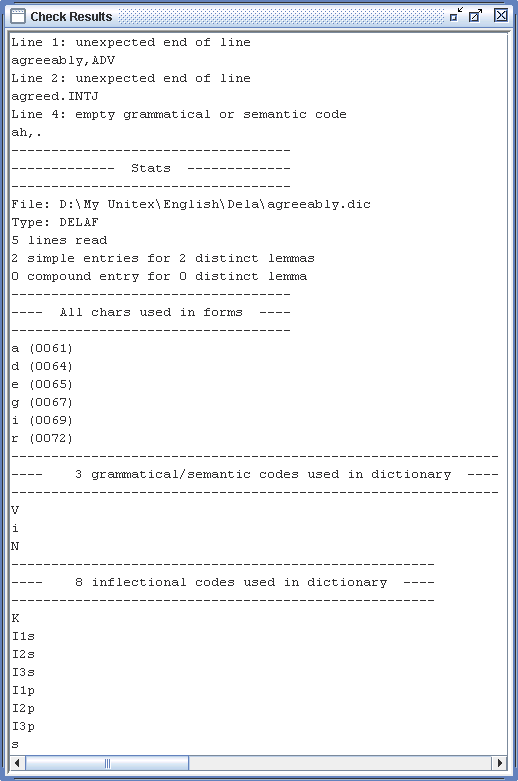
\includegraphics[width=10cm]{resources/img/fig3-4.png}
\caption{Dictionary example\label{fig-dictionary-example}}
\end{center}
\end{figure}

\noindent Let's load the dictionary as in figure~\ref{fig-dictionary-example}.
Then, click on "Check Format..." in the
"DELA" menu. A window like in
figure~\ref{fig-dictionary-checking} is opened. You
must select the type of dictionary you want to check. After checking the dictionary in Figure~\ref{fig-dictionary-example}, 
results are presented as shown in Figure~\ref{fig-dictionary-checking-results}.

\bigskip
\noindent The first error is caused by a missing period. The second, by the fact
that no comma was found after the end of an inflected form. The third error indicates
that the program didn't find any grammatical or semantic codes.



\begin{figure}[!h]
\begin{center}
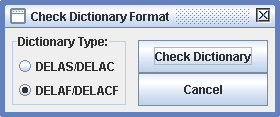
\includegraphics[width=7cm]{resources/img/fig3-5.png}
\caption{Checking a dictionary\label{fig-dictionary-checking}}
\end{center}
\end{figure}

\begin{figure}[!p]
\begin{center}
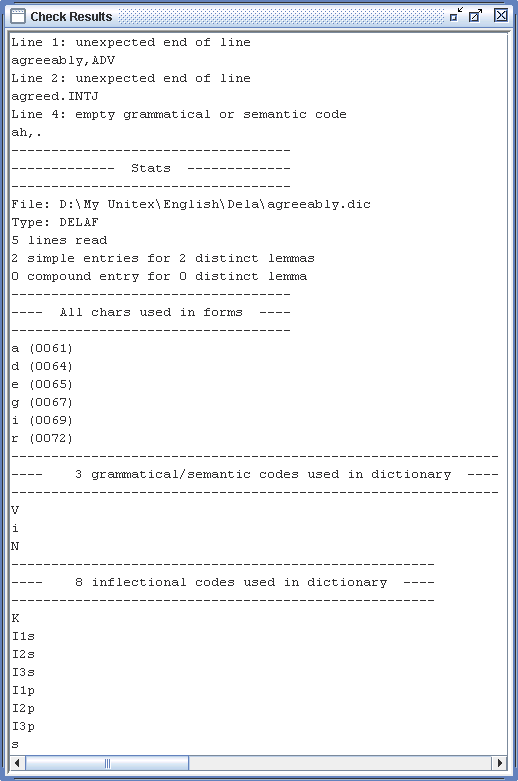
\includegraphics[height=19.4cm]{resources/img/fig3-6.png}
\caption{Results of checking\label{fig-dictionary-checking-results}}
\end{center}
\end{figure}


\section{Sorting}
\index{Dictionaries!sorting}\index{Sorting!a dictionary}

Unitex uses the dictionaries without having to worry about the order of the
entries. When displaying them it is sometimes preferable to sort the
dictionaries. The sorting depends on a number of criteria, first of all on the
language of the text. Therefore the sorting of a Thai dictionary is done
according to an order different from the alphabetical order.  So different in
fact that Unitex uses a sorting procedure developed specifically for Thai (see
chapter \ref{chap-external-programs}).

\bigskip
\noindent For European languages the sorting is usually done according to the
lexicographical order, although there are some variants. Certain languages like
French treat some characters as equivalent. For example, the difference between
the characters  \verb+e+  and \texttt{\'e}  is ignored if one wants to compare
the words \verb+manger+ et \texttt{mang\'es} because the contexts
\verb+r+ and \verb+s+ allow to decide the order. The difference is only taken 
into account when the contexts are
identical, as they are when comparing \texttt{p\^eche} and
\texttt{p\`eche}.

\bigskip \index{Alphabet!sort}
\noindent
To allow for such effect, the \verb+SortTxt+ program  
\index{\verb+SortTxt+}\index{External programs!\verb+SortTxt+} uses a file which
defines the equivalence of characters. \index{Equivalent characters}  This file
is named \verb+Alphabet_sort.txt+ \index{File!\verb+Alphabet_sort.txt+} and can
be found in the user directory for the current language. By default the first
lines of this file for French look like this:

\bigskip
\noindent
\texttt{A\`A\^A\"Aa\`a\^a\"a}

\noindent
\texttt{Bb}

\noindent
\texttt{C\c{C}c\c{c}}

\noindent
\texttt{Dd}

\noindent
\texttt{E\'E\`E\^E\"Ee\'e\`e\^e\"e}


\bigskip
\noindent Characters in the same line are considered equivalent if the context permits. If
two equivalent characters must be compared, they are sorted in the order they
appear in from left to right. As can be seen from the extract above, there is no
difference between lower and upper case. Accents and the c\'edille character are
ignored as well.

\bigskip
\noindent To sort a dictionary, open it and then click on "Sort Dictionary" in
 the "DELA" menu. By default, the program always looks for the file
\verb+Alphabet_sort.txt+. If that file doesn't exist, the sorting is done
according to the character indices in the Unicode encoding. By modifying that
file, you can define your own sorting order.

\bigskip
\noindent NOTE: After applying the dictionaries to a text, the files
\verb+dlf+, \verb+dlc+ and \verb+err+ are automatically sorted using this
program. \index{File!\verb+dlf+} \index{File!\verb+dlc+}
\index{File!\verb+err+}



\section{Automatic inflection}
\label{section-automatic-inflection}
\index{Inflection}\index{Conjugation}\index{Declension}\index{Automatic inflection}\index{Dictionaries!automatic inflection}
\subsection{Inflection of simple words}

As described in section~\ref{section-DELAS-format}, a line in a DELAS
consists of a canonical form and a sequence of grammatical or semantic codes:

\begin{verbatim}
aviatrix,N4+Hum
matrix,N4+Math
radix,N4
\end{verbatim}

\bigskip
\noindent The first code is used to determine the grammatical code of the entry as
well as the name of the grammar used to inflect the canonical form. There are
two possible forms:

\begin{itemize}
  \item \verb+N4+: grammar name=\verb+N4.fst2+, grammatical code=\verb+N+
  (longest letter prefix)
  \item \verb+N(NC_XXX)+: grammar name=\verb+NC_XXX.fst2+, grammatical code=\verb+N+
\end{itemize}

\bigskip
\noindent These inflectional grammars \index{Grammars!inflectional} will automatically be
compiled if needed. In the example above, all entries will be inflected by a grammar named \verb+N4+.

\bigskip
\noindent In order to  inflect a dictionary, click on "Inflect..." in the "DELA" menu. The
window in figure~\ref{fig-inflection-configuration} allows you to specify the
directory in which inflectional grammars are found. By default, the subdirectory
\verb+Inflection+ of the directory for the current language is used. You can
also specify the kind of words your DELAS is supposed to contain. If an entry is
found that does not correspond to your choice, an error message will be
displayed.

\bigskip
\begin{figure}[h]
\begin{center}
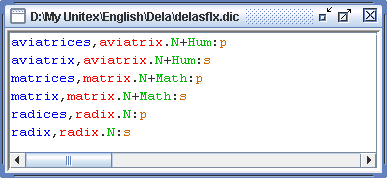
\includegraphics[width=8cm]{resources/img/fig3-7.png}
\caption{Configuration of automatic inflection\label{fig-inflection-configuration}}
\end{center}
\end{figure}

\bigskip
\begin{figure}[h]
\begin{center}
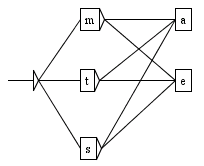
\includegraphics[width=4.5cm]{resources/img/fig3-8.png}
\caption{Inflectional grammar
\texttt{N4}\label{fig-example-inflectional-grammar}}
\end{center}
\end{figure}

\bigskip
\noindent Figure~\ref{fig-example-inflectional-grammar} shows an example of an
inflectional grammar. The paths describe the suffixes to add or to remove to
get to an inflected form from a canonical form, and the outputs (text in bold under the boxes) are the
inflectional codes to add to a dictionary entry.

\bigskip
\noindent In our example, two paths are possible. The first does not modify the
canonical form and adds the inflectional code \verb+:s+. The second deletes a letter with
the \verb+L+ operator, then adds the \verb+ces+ suffix and adds the inflectional
code \verb+:mp+. Here are the operators that can be used:
\index{\verb+L+}\index{Operator!\verb+L+}\index{\verb+R+}\index{Operator!\verb+R+}
\index{\verb+C+}\index{Operator!\verb+C+}\index{\verb+D+}\index{Operator!\verb+D+}
\index{\verb+U+}\index{Operator!\verb+U+}
\index{\verb+P+}\index{Operator!\verb+P+}
\index{\verb+W+}\index{Operator!\verb+W+}
\index{\verb+J+}\index{Operator!\verb+J+}
\index{\verb+.+}\index{Operator!\verb+.+}
\index{\verb+<R=?>+}\index{Operator!\verb+<R=?>+}
\index{\verb+<I=?>+}\index{Operator!\verb+<I=?>+}
\index{\verb+<X=n>+}\index{Operator!\verb+<X=n>+}

\begin{itemize}
  \item \verb+L+ (left) removes a letter from the entry
  
  \item \verb+R+ (right) restores a letter to the entry. In French, many verbs
  of the first group are conjugated in the present singular  of the third person form  by removing the
  \verb+r+ of the infinitive and changing the 4$^{th}$ letter from the end to
  \texttt{\`e}: \verb+peler+ $\rightarrow$ \texttt{p\`ele},
  \verb+acheter+ $\rightarrow$ \texttt{ach\`ete}, \texttt{g\'erer}
  $\rightarrow$ \texttt{g\`ere}, etc. Instead of describing an inflectional
  suffix for each verb (\texttt{LLLL\`ele}, \texttt{LLLL\`ete} and
  \texttt{LLLL\`ere}), the \verb+R+ operator can be used to
  describe it in one way: \texttt{LLLL\`eRR}.
  
  \item \verb+C+ (copy) duplicates a letter in the entry and moves everything on
  its right by one position. In cases like \verb+permitted+ or \verb+hopped+, we
  see a duplication of the final consonant of the verb. To avoid writing an
  inflectional graph for every possible final consonant, one can use the \verb+C+
  operator to duplicate any final consonant.
  
  \item \verb+D+ (delete) deletes a
  letter, shifting anything located on the right of this letter. For instance, if
  you want to inflect the Romanian word \verb+european+ into \verb+europeni+, you
  must use the sequence \verb+LDRi+. \verb+L+ will move the cursor on the
  \verb+a+, \verb+D+ will delete the \verb+a+, shifting the \verb+n+ on the left,
  and then \verb+Ri+ will restore the \verb+n+ and add an \verb+i+.

  \item \verb+U+ (unaccent) removes the accent of the current character, if
  any. For instance the sequence \verb+LLUx+ applied to the word
  \texttt{mang\'es} produces the inflected form \verb+mangex+, since \verb+U+
  has turn the \texttt{\'e} into a \verb+e+.

  \item \verb+P+ (uppercase) uppercases the initial letter of the stack. For
  instance, the sequence \verb$Px$ will turn \verb$foo$ into \verb$Foox$.
  
  \item \verb+W+ (lowercase) lowercases the initial letter of the stack.

  \item \verb+<R=?>+ replaces the initial letter of the stack by the letter \verb+?+.

  \item \verb+<I=?>+ inserts the letter \verb+?+ before the initial letter of the stack. 

  \item \verb+<X=n>+ removes the first $n$ letters of the stack. 
   
\end{itemize}

\noindent There are also two operators dedicated to Korean:
\begin{itemize}\index{Jamo}\index{Hangul}
    \item \verb+J+ removes a Jamo letter. If the current character is a Hangul
    syllab character, this character is first replaced by the equivalent Jamo
    sequence, and then, the last Jamo letter is removed. If the current
    character is neither a Jamo nor a Hangul, and error is raised.
    
    \item \verb+.+ (latin dot) inserts a syllab bound. As a side effect, if the
    top of the stack contains Jamo letters, they are first recombined into a
    Hangul character.
    \end{itemize}


\bigskip
\noindent In the example below, the inflection of \verb+choose+ is
shown. The sequence \verb+LLDRRn+ describes the form \verb+chosen+:

\begin{itemize}
  \item Step 0: the canonical form is copied on the stack, and the cursor is set behind the last letter:
  
  \begin{center}
\begin{tabular}{|l|l|l|l|l|l|l|l}
\multicolumn{6}{l}{} & \multicolumn{2}{l}{$\downarrow$} \\
\hline
\verb+c+ & \verb+h+ & \verb+o+ & \verb+o+ & \verb+s+ & \verb+e+ & \verb+ + & \\
\hline
\end{tabular}
\end{center}

\bigskip
\item Step 1: the cursor is moved one position to the left:

\begin{center}
\texttt{\textbf{L}LDRRn}

\begin{tabular}{|l|l|l|l|l|l|l|l}
\multicolumn{5}{l}{} & \multicolumn{3}{l}{$\downarrow$} \\
\hline
\verb+c+ & \verb+h+ & \verb+o+ & \verb+o+ & \verb+s+ & \verb+e+ & \verb+ + & \\
\hline
\end{tabular}
\end{center}

\bigskip
\item Step 2: the cursor is moved one position to the left again:

\begin{center}
\texttt{\textbf{LL}DRRn}

\begin{tabular}{|l|l|l|l|l|l|l|l}
\multicolumn{4}{l}{} & \multicolumn{4}{l}{$\downarrow$} \\
\hline
\verb+c+ & \verb+h+ & \verb+o+ & \verb+o+ & \verb+s+ & \verb+e+ & \verb+ + & \\
\hline
\end{tabular}
\end{center}

\bigskip \item Step 3: one character is deleted; everything to the right of the
cursor is shifted one position to the left:

\begin{center}
\texttt{\textbf{LLD}RRn}

\begin{tabular}{|l|l|l|l|l|l|l|l}
\multicolumn{3}{l}{} & \multicolumn{5}{l}{$\downarrow$} \\
\hline
\verb+c+ & \verb+h+ & \verb+o+ & \verb+s+ & \verb+e+ & \verb+ + & \verb+ + & \\
\hline
\end{tabular}
\end{center}

\bigskip
\item Step 4: the cursor is moved to the right:

\begin{center}
\texttt{\textbf{LLDR}Rn}

\begin{tabular}{|l|l|l|l|l|l|l|l}
\multicolumn{4}{l}{} & \multicolumn{4}{l}{$\downarrow$} \\
\hline
\verb+c+ & \verb+h+ & \verb+o+ & \verb+s+ & \verb+e+ & \verb+ + & \verb+ + & \\
\hline
\end{tabular}
\end{center}

\bigskip
\item Step 5: and to the right again:

\begin{center}
\texttt{\textbf{LLDRR}n}

\begin{tabular}{|l|l|l|l|l|l|l|l}
\multicolumn{5}{l}{} & \multicolumn{3}{l}{$\downarrow$} \\
\hline
\verb+c+ & \verb+h+ & \verb+o+ & \verb+s+ & \verb+e+ & \verb+ + & \verb+ + & \\
\hline
\end{tabular}
\end{center}

\bigskip
\item Step 6: the character \verb+n+ is pushed on the stack:

\begin{center}
\texttt{\textbf{LLDRRn}}

\begin{tabular}{|l|l|l|l|l|l|l|l}
\multicolumn{6}{l}{} & \multicolumn{2}{l}{$\downarrow$} \\
\hline
\verb+c+ & \verb+h+ & \verb+o+ & \verb+s+ & \verb+e+ & \verb+n+ & \verb+ + & \\
\hline
\end{tabular}
\end{center}
\end{itemize}

\bigskip
\noindent When all operations have been fulfilled, the inflected form
consists of all letters before the cursor (here \verb+chosen+).

\bigskip
\noindent The inflection program
explores all paths of the inflectional grammar and tries all possible forms. In
order to avoid having to replace the names of inflectional grammars by the actual
grammatical codes to be used in the dictionary, the program replaces these names by the
longest prefixes made of letters.
% if you have selected the "Remove class numbers" button.
Thus, \verb+N4+ is replaced by \verb+N+. By choosing the inflectional
grammar names carefully, one can construct a ready-to-use dictionary.

\bigskip
\noindent Figure \ref{fig-inflection-result} shows the dictionary we get after the inflection of 
our DELAS example.

\bigskip
\begin{figure}[!ht]
\begin{center}
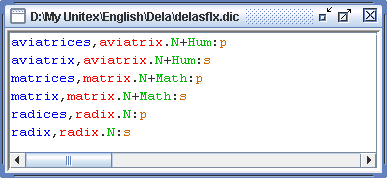
\includegraphics[width=9.5cm]{resources/img/fig3-9.png}
\caption{Result of automatic inflection\label{fig-inflection-result}}
\end{center}
\end{figure}
\subsection{Advanced inflection operators}
\label{advanced-inflection-operators}

In some languages the inflection process can modify the root of the word.
Several operators have been developped in order to facilitate this type of treatment. 
They allow to search and remove a suffix of the word \verb+W+ to be inflected.
It is also possible to store a factor of this suffix by using a special variable (\$ or ${\pounds}$).
These operators can take the following forms :

\bigskip
\begin{itemize}
\item \verb+<X$Y>+~: Starting from the end of the word \verb+W+  we are looking for the first occurrence of \verb+Y+.
	Then, we search the {\bf first} occurrence of \verb+X+ which strictly precedes that 
	of  \verb+Y+ . The \$ variable then contains the {\bf shortest factor}
	({\bf\$}hortest) of \verb+W+ strictly between \verb+X+ and \verb+Y+ (\verb+W = U.X.$.Y+)\footnote{The point
	represents here the concatenation operation.}.
\item \verb+<X+${\pounds}$\verb+Y>+~:  Starting from the end of the word \verb+W+  we are looking for the first occurrence of \verb+Y+.
	Then, we search the {\bf last} occurrence of \verb+X+ which strictly precedes that of \verb+Y+. The {\pounds}  variable then contains the  {\bf longest factor}
	({\bf${\pounds}$}ongest) of \verb+W+ strictly between \verb+X+ and \verb+Y+ (\verb+W = U.X.+${\pounds}$\verb+.Y+).
\item \verb+<X>+~: If there is no variable, we search \verb+X+ as a suffix of \verb+W+
	(\verb+W = U.X+).
\item \verb+<$Y>+: If the \verb+X+ factor is absent, the {\bf shortest factor \verb+$+} is the first letter which strictly precedes \verb+Y+ .
\item \verb+<+${\pounds}$\verb+Y>+~: If the \verb+X+ factor is absent, the {\bf longest factor ${\pounds}$} is the prefix of
	\verb+W+ so that  \verb+W = +${\pounds}$ \verb+.Y+.
\end{itemize}

\bigskip
\noindent
To illustrate the use of these operators, let us consider the french verb {\it reprendre}~:

\bigskip
\begin{center}
\begin{tabular}{|l|l|l|l|}
\hline
Word     & Operator & Variable & Result\\
\hline
\hline
reprendre & <re> & & reprend\\
reprendre & <\$> & \$ = e & reprendr\\
reprendre & <{\pounds}> &{\pounds}= reprendre & $\varepsilon$ \\
reprendre & <re\$re> & \$ = nd & rep\\
reprendre & <re{\pounds}re> & {\pounds} = prend & \\
reprendre & <\$re> & \$ = d & repren\\
reprendre & <re\$> & \$ =  $\varepsilon$ & reprendre\\
reprendre & <{\pounds}re> & {\pounds} = reprend & $\varepsilon$\\
reprendre & <re{\pounds}> & {\pounds} = prendre & re\\
\hline
\end{tabular}
\end{center}

\bigskip
\noindent
The MultiFlex program allows you to use ten variables of type \$ whose names are \$,\$1,...,\$9
and ten variables of type {\pounds} whose names are {\pounds},{\pounds}1,...,{\pounds}9.
Morever, both types of variables can be mixed in a same operator. Thus the operator <{\pounds}3re\$7re>
applied to the french verb {\it reprendre} gives back~: {\pounds}3 = rep et \$7 = \verb+nd+.

\bigskip
\noindent
In the verbs \verb+accélérer+, \verb+sécher+, the second person of the present tense
can be generated by the operation <é\$er>è\$es~:

\begin{center}
\begin{tabular}{lllllllll}
	\verb+accélérer+ & <é\$er> & $\rightarrow$ & accél & \$ = r & + & è\$es &  $\rightarrow$ & \verb+accélères+\\
	\verb+sécher+ & <é\$er> & $\rightarrow$ & s & \$ = ch & + & è\$es & $\rightarrow$ & \verb+sèches+\\
\end{tabular}
\end{center}

%\bigskip
\noindent
Note that the factor \verb+$+ which remains in the inflected form is of variable length (\verb+r+, \verb+ch+). 
The inflection of the verbs \verb+accélérer+ and \verb+sécher+ cannot be done with classical stack operators
within the same operation. Two different operations (\verb+-4RèCes+, \verb+-5RèCes+) are
needed. The graph shown in figure~\ref{fig-inflection-secher} inflects verbs like
\verb+accélérer+ and \verb+sécher+ in the present tense.

%\bigskip
\begin{figure}[!ht]
\begin{center}
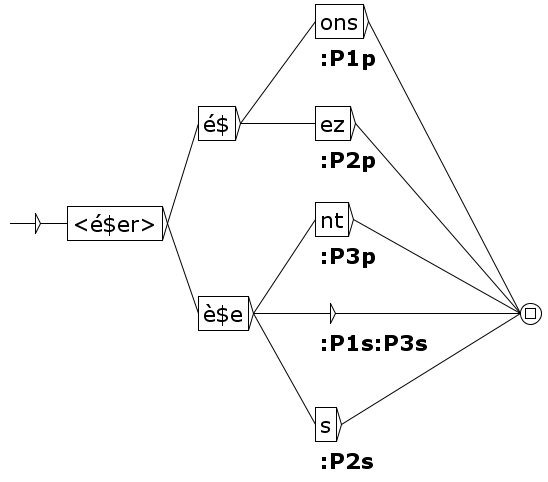
\includegraphics[width=7cm]{resources/img/fig3-Advanced_operators_with_Variables-V_secher.png}
\caption{Inflection graph for verbs like {\it accélérer}, {\it sécher}
\label{fig-inflection-secher}}
\end{center}
\end{figure}

\newpage
%\bigskip
\noindent
The inflected forms of the verbs \verb+accélérer+ and \verb+sécher+ are~:

%\bigskip
\begin{figure}[!ht]
\begin{center}
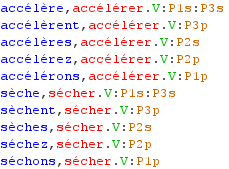
\includegraphics[width=5cm]{resources/img/fig3-flexion_secher.png}
\end{center}
\end{figure}

\bigskip
\noindent
The doubling of some letters during the inflection process can be done with the operator \$.
For example the adjective {\it tranquil} has two forms in the comparative and two in the 
superlative. The graph in figure ~\ref{fig-inflection-tranquil} can produce these forms.

\bigskip
\begin{figure}[!ht]
\begin{center}
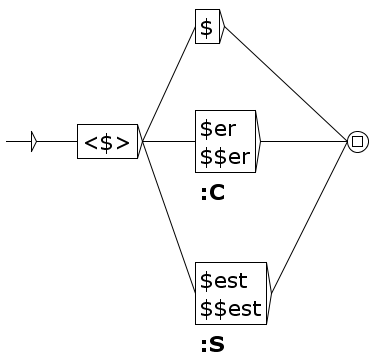
\includegraphics[width=5.5cm]{resources/img/fig3-Advanced_operators_with_Variables-A_tranquil.png}
\caption{Inflection graph for adjectives like {\it tranquil}
\label{fig-inflection-tranquil}}
\end{center}
\end{figure}

\noindent Below are the inflected forms for the adjective \verb+tranquil+~:

\bigskip
\begin{figure}[!ht]
\begin{center}
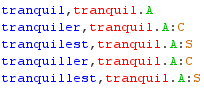
\includegraphics[width=5cm]{resources/img/fig3-flexion_tranquil.png}
\end{center}
\end{figure}

%\bigskip
\noindent  In some languages, some inflected forms have a prefix added before the root like the formation of the past participle in German. The joint use of operators
${\pounds}$ et \verb+$+ allows to inflect the german verb \verb+sprechen+ (to speak)
in the present tense and the past participle as shown in the graph in figure~\ref{fig-inflection-sprechen}.

\newpage
%\bigskip
\begin{figure}[!htbp]
\begin{center}
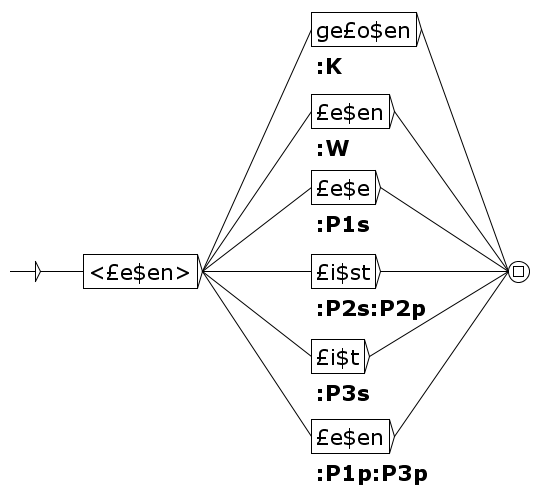
\includegraphics[width=5cm]{resources/img/fig3-Advanced_operators_with_Variables-V_sprechen.png}
\caption{Inflection graph for verbs like {\it sprechen}
\label{fig-inflection-sprechen}}
\end{center}
\end{figure}

%\bigskip
\noindent The inflection forms of the verb \verb+sprechen+~:

\bigskip
\begin{figure}[!ht]
\begin{center}
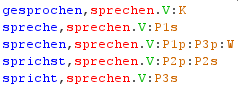
\includegraphics[width=5cm]{resources/img/fig3-flexion_sprechen.png}
\end{center}
\end{figure}

%\bigskip
\noindent In order to inflect the phrasal verb  \verb+aussprechen+  two variables of type \$ should be used.
Figure ~\ref{fig-inflection-aussprechen} shows a graph with two variables \verb+$1+ and \verb+$2+.

\bigskip
\begin{figure}[!ht]
\begin{center}
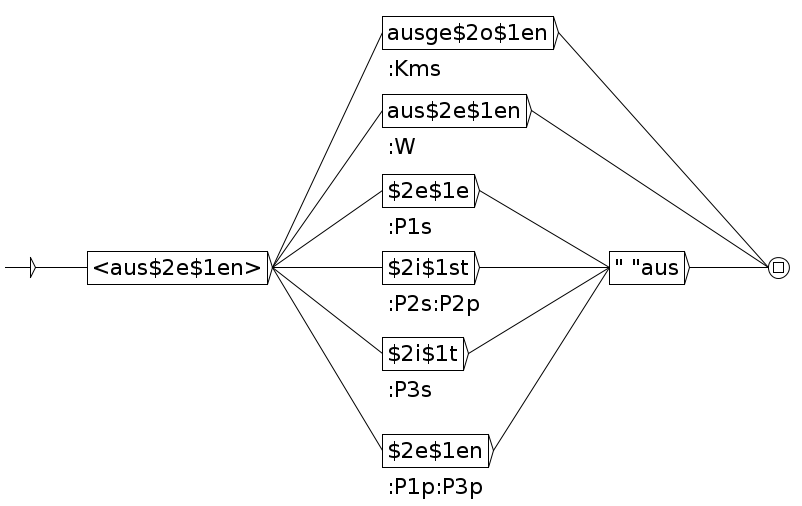
\includegraphics[width=10.5cm]{resources/img/fig3-Advanced_operators_with_Variables-V_aussprechen.png}
\caption{Inflection graph for verbs like {\it aussprechen}
\label{fig-inflection-aussprechen}}
\end{center}
\end{figure}

\noindent Here are the inflection forms of the verb \verb+aussprechen+~:
\bigskip
\begin{figure}[!ht]
\begin{center}
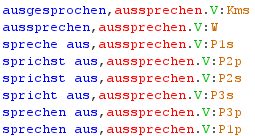
\includegraphics[width=5cm]{resources/img/fig3-flexion_aussprechen2.png}
\end{center}
\end{figure}

\bigskip
\noindent \textbf{Semantic codes}

\noindent In some languages, there are inflectional features that actually correspond to 
semantic ones, like for instance markers for the passive form. Such codes may not appear
as inflectional ones, but rather as semantic ones. To do that and produce semantic codes, 
you have to insert a plus sign at the beginning of the output of a box. The box must only 
contain the semantic code preceeded by a plus, as shown on Figure \ref{fig-inflection-sem}.

\bigskip
\begin{figure}[!ht]
\begin{center}
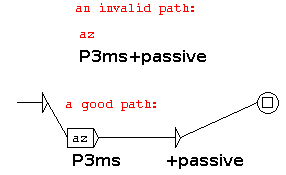
\includegraphics[width=6cm]{resources/img/fig3-9sem.png}
\caption{An inflection grammar with a semantic code\label{fig-inflection-sem}}
\end{center}
\end{figure}

\subsection{Inflection of compound words}
See chapter \ref{chap-multiflex}.

\subsection{Inflection of semitic languages}
\label{subsection-semitic-inflection}
\index{Semitic languages}
Semitic languages like Arabic or Hebrew are not inflected in the same way as 
other types of languages. Their morphology obeys a different logic. In
 such languages, words are inflected according to \textit{consonant
skeletons}\index{Consonant skeleton}. The
inflection process combines this skeleton with vowels.

\bigskip
\noindent First, let us see a case where we encode only the consonants in the lemma field of the DELAS  entry:

\bigskip
\noindent \verb+ktb,$V31-123+

\bigskip
\noindent The \verb+$+ sign before the grammatical code indicates that the inflection grammar 
is in the Semitic mode, and the form \verb+ktb+ in the lemma field is the consonant
skeleton. Figure~\ref{semitic-grammar} shows the toy grammar \verb+V31-123.grf+
that illustrates how the Semitic mode works.  

\bigskip
\begin{figure}[!ht]
\begin{center}
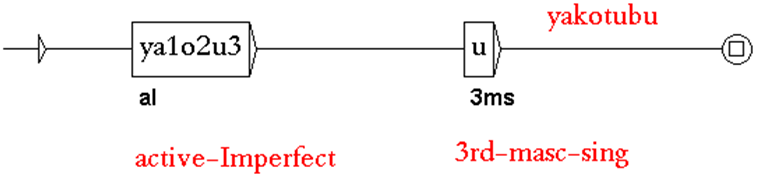
\includegraphics[width=10cm]{resources/img/fig3-15.png}
\caption{A toy inflection grammar\label{semitic-grammar} in the Semitic mode}
\end{center}
\end{figure}

\bigskip
\noindent The Semitic mode obeys the following rules:
\begin{enumerate}
  \item All standard inflection operators can be used (\verb+L+, \verb+R+, etc).
  \item A digit stands for a letter in the lemma field (\verb+1+ for the first,
  \verb+2+ for the second, etc). In our example, \verb+1+, \verb+2+ and
  \verb+3+ will respectively stand for \verb+k+, \verb+t+ and
  \verb+b+. If you want to access to a letter after the ninth one, you must
  protect its index with angles like \verb+<10>+.
\end{enumerate}  

\bigskip
\noindent The DELAF output for this grammar is: 
  
\verb+yakotubu,ktb.V:aI3ms+

\bigskip
\noindent If we encode only the consonants in the lemma field and  two entries have the same consonants
but differ in the vowels, we must encode the vowels in the inflection grammars:

\verb+Hsb,$V3au	// to count, Hasaba, yaHosubu+

\verb+Hsb,$V3ii	// to think, Hasiba, yaHosibu+

\bigskip
\noindent In order to copy the complete lemma field, use the <LEMMA> operator (Figure~\ref{LEMMA-operator}).

\begin{figure}[!ht]
\begin{center}
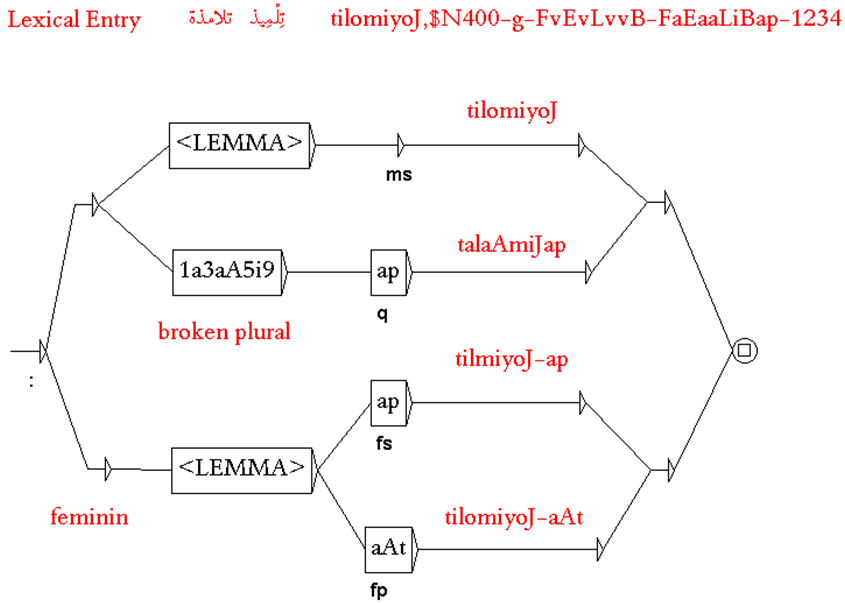
\includegraphics[width=10cm]{resources/img/fig3-LEMMA-operator.png}
\caption{An inflection grammar in the Semitic mode with the <LEMMA> operator\label{LEMMA-operator}}
\end{center}
\end{figure}

\noindent Thus, a path with all this field does not depend on the number of letters in the field. This operator is useful for
Arabic nouns and adjectives where masculine forms are generated by inserting vowels in the consonantal skeleton, whereas feminine forms are obtained by appending suffixes. In this example, both consonants and vowels are encoded in the lemma field.

\section{Compression}
\index{Dictionaries!compression}

Unitex applies compressed dictionaries to the text. The compression reduces the
size of the dictionaries and speeds up the lookup. This operation is done by the
\verb+Compress+ program. \index{\verb+Compress+}\index{External
programs!\verb+Compress+}This program takes a dictionary in text form 
as input (for example \verb+my_dico.dic+) and produces two files:

\index{File!\verb+.dic+}
\begin{itemize}
  \item \verb+my_dico.bin+ contains the minimal automaton of the inflected forms of the dictionaries;
  \index{File!\verb+.bin+}
  \item \verb+my_dico.inf+ contains the codes extracted from the original dictionary.\index{File!\verb+.inf+}
\end{itemize}

\index{Automaton!minimal}
\noindent The minimal automaton in the \verb+my_dico.bin+ file is a
representation of inflected forms in which all common prefixes and suffixes are factorized. For
example, the minimal automaton of the words \verb+me+, \verb+te+, \verb+se+,
\verb+ma+, \verb+ta+ et \verb+sa+ can be represented by the graph shown in
Figure~\ref{fig-example-minimal-automaton}. \bigskip \begin{figure}[!h]
\begin{center}
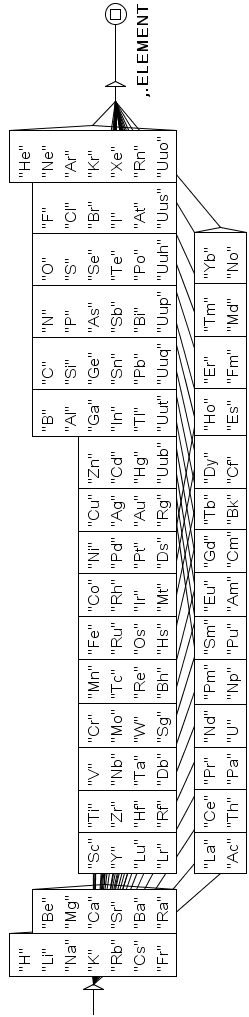
\includegraphics[width=5cm]{resources/img/fig3-10.png}
\caption{Representation of a minimal
automaton\label{fig-example-minimal-automaton}}
\end{center}
\end{figure}

\noindent To compress a dictionary, open it and click on "Compress into FST" in
the "DELA" menu. The compression is independent from the language and from the content of
the dictionary. The messages produced by the program are displayed in a window
that is not closed automatically. You can see the size of the resulting
\verb+.bin+ file, the number of lines read and the number of inflectional codes
created. Figure~\ref{fig-compression-result} shows the result of
the compression of a dictionary of simple words. \bigskip
\begin{figure}[!h]
\begin{center}
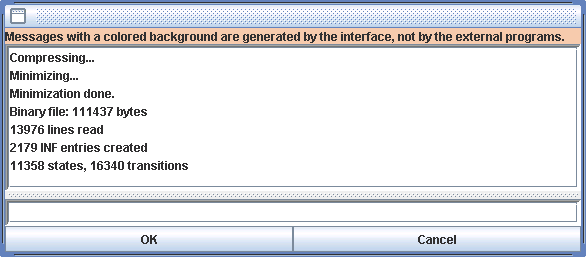
\includegraphics[width=14cm]{resources/img/fig3-11.png}
\caption{Results of a compression\label{fig-compression-result}}
\end{center}
\end{figure}

\bigskip
\noindent The resulting files are compressed to about 95\% for dictionaries containing
simple words and 50\% for those with compound words.

\bigskip
\noindent NOTE: for semitic languages, a special compression algorithm is used to reduce the size of
                the output \verb+.bin+ and \verb+.inf+ files. The fact that a language is considered as
                a semitic one can be configured in the global preferences.
\section{Applying dictionaries}
\label{section-applying-dictionaries}
\index{Dictionaries!applying}
Dictionaries can be applied (1) after pre-processing or (2) by explicitly 
clicking on "Apply Lexical Resources" in the  "Text" menu (see
section~\ref{text-applying-dictionaries}).

\bigskip
\noindent Unitex can manipulate compressed dictionaries (\verb+.bin+) and
dictionary graphs (\verb+.fst2+). We will now describe  the rules for applying dictionaries
in detail. Dictionary graphs will be described in
section~\ref{section-dictionary-graphs}.

\subsection{Priorities}
\label{section-dictionary-priorities}
\index{Dictionaries!priority}\index{Priority!of dictionaries}
The priority rule says that  if a word in a text is found in a dictionary, this
word will not be taken into account by dictionaries with lower priority.

\bigskip
\noindent This allows for eliminating a part of ambiguity when applying
dictionaries. For example, the French word \textit{par} has a nominal interpretation in the golf
domain. If you don't want to use this meaning, it is sufficient to create a
filter dictionary containing only the entry \verb$par,.PREP$ and to apply this
with highest priority. This way, even if simple word dictionaries contain 
different entries, they will be ignored given the priority rule.
\index{Dictionaries!filters}

\bigskip
\noindent There are three priority levels. The dictionaries whose names without
extension end with~\verb+-+
\index{\verb+-+}\index{\verb-+-}
have the highest priority; those that end with~\verb-+- have the lowest one.
All other dictionaries are applied with medium priority. The order in which
dictionaries with the same priority are applied does not matter.
On the command line, the command:

\bigskip
\noindent
\verb$Dico ex.snt alph.txt ctr+.bin cities-.bin rivers.bin regions-.bin$

\bigskip \noindent will apply the dictionaries in the following order
(\verb+ex.snt+ is the text to which the dictionaries are applied, and 
\verb+alph.txt+ is the alphabet file used):

\bigskip
\begin{enumerate}
  \item \verb$cities-.bin$
  \item \verb$regions-.bin$
  \item \verb$rivers.bin$
  \item \verb$ctr+.bin$
\end{enumerate}

\subsection{Application rules for dictionaries}
\label{section-transducer-application-rules}

Besides the priority rule, the application of dictionaries respects  upper  case
letters and spaces. The upper case rule is as follows:
\index{Rules!upper case and lower case letters}

\begin{itemize}
  \item if there is an upper case letter in the dictionary, then an upper case
  letter has to be in the text;
  
  \item if a lower case letter is in the dictionary, there can be either an upper
  or lower case letter in the text.
\end{itemize}

\bigskip
\noindent Thus, the entry \verb$peter,.N:fs$ will match the words \verb+peter+,
\verb+Peter+ et \verb+PETER+, while

% do not remove this line jump
\noindent \verb$Peter,.N+firstName$ only 
recognizes \verb+Peter+ and \verb+PETER+. Lower and upper case
letters are defined in the alphabet file passed to the \verb+Dico+ program\index{\verb+Dico+}
\index{External programs!\verb+Dico+}\index{File!\verb+alphabet+} as a parameter.

\index{Rules!white space}
\bigskip
\noindent Respecting white space is a very simple rule: For each sequence in the text to be
recognized by a dictionary entry, it has to have exactly the same number of
spaces. For example, if the dictionary contains \verb+aujourd'hui,.ADV+, the
sequence \verb+Aujourd' hui+ will not be recognized because of the space that
follows the apostrophe.


\subsection{Dictionary graphs}
\label{section-dictionary-graphs}\index{Dictionary graphs}
The \verb+Dico+\index{\verb+Dico+}\index{External programs!\verb+Dico+} program
can also apply dictionary graphs. Dictionary graphs conform to the following
rule: if applied by \verb+Locate+\index{\verb+Locate+}\index{External
programs!\verb+Locate+} in MERGE\index{MERGE} mode,
they must produce output sequences that are valid DELAF lines.\index{DELAF}\index{Dictionaries!DELAF}

\begin{figure}[!p]
\begin{center}
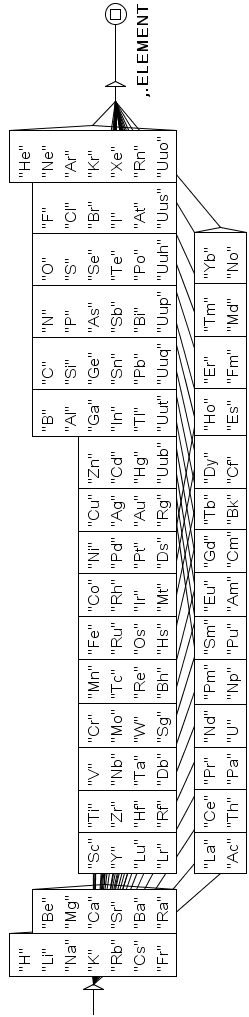
\includegraphics[height=24cm]{resources/img/fig3-12.png}
\caption{Dictionary graph of chemical elements\label{elements}}
\end{center}
\end{figure}

\bigskip
\noindent Figure \ref{elements} shows a graph that recognizes chemical
elements. We can observe a first advantage of graphs over usual dictionaries: we can force case
with double quotes. Thus, this graph will
correctly match \verb+Fe+ but not \verb+FE+, while this restriction cannot be specified in a
normal DELAF.

\bigskip
\noindent Another advantage of dictionary graphs is that they can use results
given by previous dictionaries. Thus, it is possible to apply the standard dictionary, and then tag as proper
names all the unknown words that begin with an uppercase letter, thanks to
graph \verb$NPr+$ shown in figure~\ref{graph-NPr}. The \verb$+$ in the graph
name gives to it a low priority, so that it will be applied after the standard
dictionary. This graph works with words that are still unknown after the
application of the standard dictionary. Square brackets stand for a context definition.
For more information about contexts,\index{Context} see section
\ref{section-contexts}.

\begin{figure}[!h]
\begin{center}
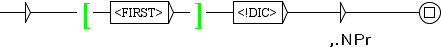
\includegraphics[width=10.5cm]{resources/img/fig3-13.png}
\caption{Dictionary graph that tags unknown words beginning with an uppercase letter as proper names\label{graph-NPr}}
\end{center}
\end{figure}

\bigskip
\noindent Since dictionary graphs are applied using the engine of \verb+Locate+,
they have exactly the same properties than syntactic graphs. So,
you can use morphological filters and/or the morphological mode.
\index{Morphological filters}\index{Morphological mode}For instance, the
graph shown on Figure \ref{graph-CR} uses morphological filters to recognize
roman numerals. Note that it also uses contexts in order to avoid recognizing 
uppercase letters in some contexts.


\bigskip
\begin{figure}[!p]
\begin{center}
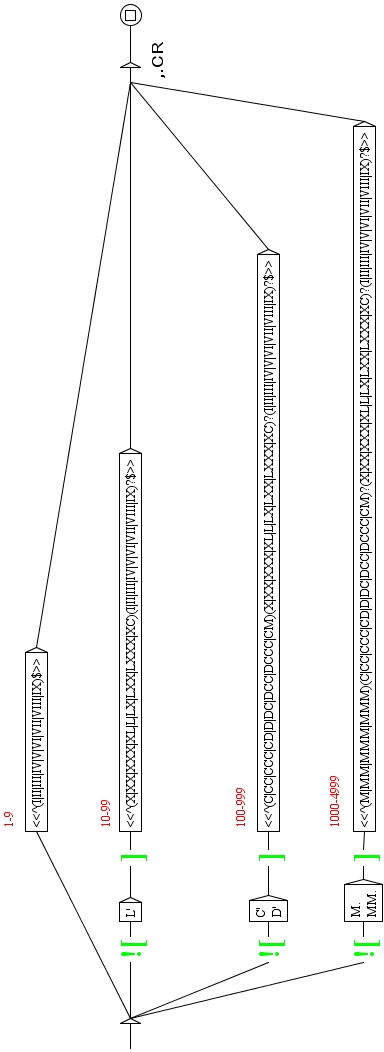
\includegraphics[height=24cm]{resources/img/fig3-14.png}
\caption{Dictionary graph of roman numerals\label{graph-CR}}
\end{center}
\end{figure}

\bigskip
\noindent By default, dictionary graphs are applied in MERGE mode. If you want
to apply them in REPLACE mode, you must suffix graph names with \verb+-r+. This can
be combined with the \verb-+- and \verb+-+ priority marks:

\bigskip
\verb?bagpipe-r.fst2  McAdam-r-.fst2  phtirius-r+.fst2?

\subsubsection{Exporting produced entries as a morphological-mode dictionary}
\index{Morphological-mode dictionaries}
Dictionary entries produced by dictionary graphs are, of course, taken
into account by the \verb+Locate+ program. However, you can not refer to 
their content while in the morphological mode, since they do not belong to a morphological-mode 
dictionary. If you want to do so, you just have to add \verb+b+ at the end of
the graph name. If you add \verb+z+ instead, then the dictionary generated for the text
will be compressed immediately, thus being usable by the next dictionary graph 
to be applied.
 
\subsubsection{Naming conventions}
The whole naming scheme for dictionary graphs is as follows:

\verb$name(-XYZ)([-+]).fst2$

\noindent where:
\begin{itemize}
\item \verb+X+ is in \verb+[rRmM]+: \verb+r+ means REPLACE mode; \verb+M+ means MERGE mode (default);
\item \verb+Y+ is in \verb+[bBzZ]+: option that rules the production of a morphological-mode dictionary (see above);
\item \verb+Z+ is in \verb+[aAlLsS]+: \verb+a+ means that the graph will be applied in "All matches" mode; \verb+l+ means 
      "Longest matches" mode (default); \verb+s+ means "Shortest matches" mode.
\end{itemize}



\subsection{Morphological dictionary-graphs}
\index{Morphological dictionary-graphs}
In addition to dictionary graphs that produce new entries in the text
dictionaries, you can design morphological dictionary-graphs. The output
of such graphs will be used as special input for the construction of the text
automaton. We call them `morphological dictionary-graphs' because their
main utility is to introduce new morphological analyses in the text automaton,
using the morphological mode (see section \ref{section-morphological-mode}).
This functionality will be helpful for agglutinative languages like Korean.

\bigskip
\noindent The rule is simple: any output of a dictionary graph that begins
with a slash will be added to the file \verb+tags.ind+, \index{\verb+tags.ind+}
located in the text directory. This file is used by the \verb+Txt2Fst2+ program
in order to add interpretations into the text automaton. Let us consider the
grammar shown on Figure \ref{morphoA} that matches words made of the prefix
\verb+un+ followed by an adjective. If we apply this grammar as a dictionary
graph, we obtain new paths in the text automaton, as shown on Figure
\ref{morphoB}. Note that when two tags correspond to analyses within the same
token, the link between them is displayed with a dashed line.

\begin{figure}[!ht]
\begin{center}
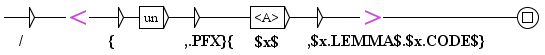
\includegraphics[width=14cm]{resources/img/fig3-14a.png}
\caption{Example of a morphological dictionary-graph\label{morphoA}}
\end{center}
\end{figure}

\begin{figure}[!ht]
\begin{center}
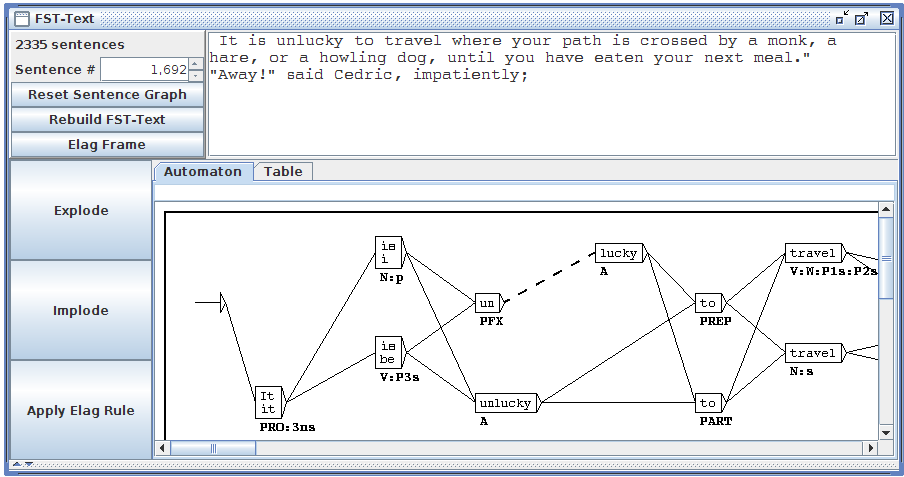
\includegraphics[width=15cm]{resources/img/fig3-14b.png}
\caption{Path added by a morphological dictionary-graph\label{morphoB}}
\end{center}
\end{figure}


\section{Bibliography}


Table~\ref{ref-dicos} gives some references for electronic dictionaries with simple and 
compound words. For more details, see the references page on the Unitex website: \\
\url{http://www-igm.univ-mlv.fr/~unitex}

\begin{table}[!h]
\begin{center}
\begin{tabular}{|l|c|c|}
\hline
\textbf{Language} & \textbf{Simple words} & \textbf{Compound words} \\
\hline
English & \cite{klarsfeld}, \cite{monceaux-1995} & \cite{delac-anglais},
\cite{these-Savary} \\
\hline
French & \cite{formes-ambigues}, \cite{dicos-francais}, \cite{jacques-1995} & \cite{dicos-francais},
\cite{Gross96},
\cite{max-1993},
\cite{syntaxe-de-ladverbe} \\
\hline
Modern Greek & \cite{modern-greek}, \cite{matthieu-anastasia}, \cite{these-tita} & \cite{tita-2002},
\cite{anastasia-2002} \\
\hline
Italian & \cite{delaf-italien}, \cite{delaf-italien-book} & \cite{composes-italien} \\
\hline
Spanish & \cite{blanco-2000} & \cite{blanco-1997} \\
\hline
Portuguese & \cite{eleuterio1995}, \cite{ranchhod1996b}, \cite{ranchhodd1998},
\cite{muniz2005} & \cite{ranchhod1991}, \cite{ranchhodd1998} \\
\hline
\end{tabular}
\caption{Some bibliographical references for electronic dictionaries\label{ref-dicos}}
\end{center}
\end{table}

\chapter{Searching with regular expressions}
\label{chap-regexp}

This chapter describes how to search a text for simple patterns by using regular
expressions.

\section{Definition}
\index{Regular expressions}

The goal of this chapter is not to give an introduction on formal languages but
to show how to use regular expressions in Unitex in order to search for simple
patterns. Readers who are interested in a more formal presentation can consult
the many works that discuss regular expression patterns.

\bigskip \noindent A regular expression can be:

\begin{itemize}
  \item a token (\verb+book+) or a lexical mask
  (\verb+<smoke.V>+);
  \item a particular position in the text : the beginning \verb+{^}+ or the end \verb+{$}+
  \item the concatenation of two regular
  expressions (\verb+he smokes+);\index{Concatenation of regular expressions}
  \item the union of two regular expressions
  (\verb$Pierre+Paul$);\index{Union of regular expressions} 
  \item the Kleene star of a regular expression
  (\verb+bye*+).\index{Kleene star}
\end{itemize}





\section{Tokens}
\index{Token}

In a regular expression, a token is defined as in \ref{tokenization} (page
\pageref{tokenization}). Note that the symbols dot, plus,
star, less than, opening and closing parentheses and double quotes have a
special meaning. It is therefore necessary to precede them with an escape character
\verb+\+ if you want to search for them. Here are some examples of valid
tokens: \index{\verbt{\textbackslash~}}

\begin{verbatim}
cat
\.
<N:ms>
{S}
\end{verbatim}

\index{Case sensitivity}
\noindent By default, Unitex is set up to let lower case patterns also find
upper-case matches. It is possibe to enforce case-sensitive matching using quotation marks. Thus,
\verb+"peter"+ recognizes only the form \verb+peter+ and not \verb+Peter+
or \verb+PETER+.

\bigskip
\noindent NOTE: in order to make a space obligatory, it needs to  be  enclosed 
in quotation marks.
\index{Space!obligatory}


\section{Lexical masks}
\index{Lexical!mask}
A lexical mask is a search query that matches tokens or sequences of tokens.

\subsection{Special symbols}
\label{section-special-symbols}
\index{Meta-symbols}

There are two kinds of lexical masks. The first category contains the special symbols or meta-symbols 
introduced in section~\ref{section-sentence-splitting} except for \verb$<PNC>$ and \verb+<^>+.
(The symbol \verb$<PNC>$, which matches punctuation signs, is valid only
during preprocessing; \verb+<^>+ matches a line feed, but
since all line feeds have been replaced by spaces, this symbol cannot be
useful anymore when searching for lexical masks.) The meta-symbols that can be used to search a text for patterns are
the following:

\index{\verbc{<MOT>}}\index{\verbc{<MIN>}}\index{\verbc{<MAJ>}}\index{\verbc{<PRE>}}\index{\verbc{<NB>}}
\index{\verbt{\#}}\index{\verbc{<E>}}\index{\verbc{<DIC>}}\index{\verbc{<SDIC>}}\index{\verbc{<CDIC>}}
\index{\verbc{<TDIC>}}\index{\verbc{<WORD>}}\index{\verbc{<UPPER>}}\index{\verbc{<LOWER>}}\index{\verbc{<FIRST>}}
\begin{itemize}
  \item \verb+<E>+: the empty word or epsilon. Matches the empty string;
  \item \verb+<TOKEN>+: matches any token, except the space; used by default
  for morphological filters
  \item \verb+<WORD>+: matches any token that consists of letters;
  \item \verb+<LOWER>+: matches any lower-case token;
  \item \verb+<UPPER>+: matches any upper-case token;
  \item \verb+<FIRST>+: matches any token that consists of letters and starts
  with a capital lette;
  \item \verb+<DIC>+: matches any word that is present in the dictionaries of
  the text;
  \item \verb+<SDIC>+: matches any simple word in the text
  dictionaries;\index{Words!simple}
  \item \verb+<CDIC>+: matches any composed word in the dictionaries of the
  text;\index{Words!compound}
  \item \verb+<TDIC>+: matches any tagged token like \verb+{XXX,XXX.XXX}+;
  \item \verb+<NB>+: matches any contiguous sequence of digit (1234 is matched
  but not 1 234);
  \item \verb+#+: prohibits the presence of space.\index{Space!prohibited}
\end{itemize}

\noindent Earlier codes for \verb+<WORD>+, \verb+<LOWER>+, \verb+<UPPER>+ and \verb+<FIRST>+
were respectively \verb+<MOT>+, \verb+<MIN>+, \verb+<MAJ>+ and \verb+<PRE>+.
They can still be used for backward compatibility of the system with existing graphs,
but they are now deprecated, i.e.\ it is recommended to avoid them in graphs designed to be used with
more recent versions,\footnote{From version 3.1beta, revision 4072, October 2, 2015.}
so that the number of lexical masks in use does not increase uselessly.

\bigskip
\noindent NOTE: as described in section \ref{tokenization}, NO meta can be used
to match the \verb+{STOP}+\index{\verbt{\{STOP\}}} marker, not even \verb+<TOKEN>+.

\subsection{References to information in the dictionaries}
\index{Reference to information in the dictionaries}\index{Dictionaries!reference to information in the}


The second kind of lexical masks refers to the information in the
text dictionaries.
\index{Dictionaries!of the text} The four possible forms are:

\bigskip
\begin{itemize}
  \item \verb+<be>+: matches all the entries that have \verb+be+ as canonical
  form. Note that this pattern is ambiguous if \verb+be+ is also a grammatical
  or semantic code;
  \item \verb+<be.>+: matches all the entries that have \verb+be+ as canonical
  form. This pattern is not ambiguous as the previous one;
  \item \verb+<be.V>+: matches all entries having \verb+be+ as canonical form
  and the grammatical code \verb+V+;
  \item \verb+<V>+: matches all entries having the grammatical code \verb+V+.
  This pattern is as ambiguous as the first one. To remove the ambiguity, you
  can use either \verb+<.V>+ or \verb$<+V>$; 
  \index{Lexical!labels}
  \item \verb+{am,be.V} or <am,be.V>+: matches all the entries having
  \verb+am+ as inflected form, \verb+be+ as canonical form and the
  grammatical code \verb+V+. This kind of lexical mask is only of interest if applied
  to the text automaton where all the ambiguity of the words is explicit.
  \index{Text!automaton of the}\index{Automaton!of the text} While executing a
  search on the text, that lexical mask matches the same as the simple token
  \verb+am+.
\end{itemize}

\subsection{Grammatical and semantic constraints}

The references to dictionary information (\verb+be+, \verb+V+) in these examples
are basic. It is possible to express more complex lexical masks by using
several grammatical or semantic codes separated by the character \verb$+$.
If several codes are present, the character \verb$+$ means `'and'':
 an entry of the dictionary is only found if it has all the codes that are
present in the mask. The mask \verb$<N+z1>$ thus recognizes the entries:

\bigskip
\noindent
\texttt{broderies,broderie.N+z1:fp}

\noindent
\texttt{capitales europ\'eennes,capitale europ\'eenne.N+NA+Conc+HumColl+z1:fp}

\bigskip
\noindent but not:

\bigskip
\noindent
\texttt{Descartes,Ren\'e Descartes.N+Hum+NPropre:ms}

\noindent
\texttt{habitu\'e,.A+z1:ms}

\bigskip
\noindent It is possible to exclude codes by preceding them with the character \verb+~+
instead of \verb$+$.\index{Negation!of a feature}
In order to be recognized, an entry has to contain all the
codes required by the lexical mask and none of the prohibited ones. For instance,
\verb+<A~z3>+ matches the entries that have the code \verb+A+ without the code
\verb+z3+ (cf. table~\ref{tab-semantic-codes}).\footnote{If a word is described in the
dictionaries by an entry with \texttt{A+z3} and another with only \texttt{A}, the word
is matched by \texttt{<A+z3>} because of the former entry and by
\texttt{<A{\textasciitilde}z3>} because of the latter.}
If you want to refer to a code containing the character \verb$~$ you have to
escape this character by preceding it with a \verb+\+. 

\bigskip
\noindent CHANGE NOTE: before version 2.1, the negation operator was the minus. If you want
                       to preserve backward compatibility without modifying your graphs, you have
                       to call \verb+Locate+ by hand with the \verb+-g minus+ option.
\index{Exclusion of grammatical and semantic codes}\index{\verbt{\textasciitilde~}}

\bigskip
\noindent The syntax of lexical masks does not make any difference between grammatical codes
(table~\ref{tab-grammatical-codes}) and semantic codes (table~\ref{tab-semantic-codes}).
In the DELAF dictionary format, grammatical codes are those that appear first and
encode the part of speech, but in Unitex lexical masks,
the order in which grammatical and semantic codes appear does not matter. The
three following patterns are equivalent:

\begin{verbatim}
<N~Hum+z1>
<z1+N~Hum>
<~Hum+z1+N>
\end{verbatim}

\noindent A lexical mask can contain a semantic code without a part-of-speech code.

\bigskip
\noindent NOTE: it is not possible to use a lexical mask that only has
prohibited codes. \verb+<~N>+ and \verb+<~A~z1>+ are thus incorrect masks. 
However, you can express
such constraints using contexts (see section~\ref{section-contexts}).


\subsection{Inflectional constraints}
\index{Inflectional constraints}
It is also possible to specify constraints about inflectional codes. These
constraints have to be preceded by at least one grammatical or semantic code.
They are represented in the same format as the inflectional codes in the dictionaries.
Here are some French examples of lexical masks using inflectional
constraints:

\begin{itemize}
  \item \verb+<A:m>+ recognizes a adjective in the masculine;
  \item \verb+<A:mp>+ recognizes an adjective in the masculine plural.
\end{itemize}

\noindent An inflectional code is introduced by the \verb+:+ character and
is made up of one or more characters, each of which represents one piece of
information. Let us consider first the simple case of dictionary entries and masks
which have exactly one inflectional code.
In order to let a dictionary entry $E$ be recognized by a mask $M$, it
is necessary that the inflectional code of $E$ contains all the characters
of the inflectional code of $M$:

\bigskip
$E$=\verb$pretext,.V:P3p$

$M$=\verb$<V:P3>$

\bigskip
\noindent The inflectional code \verb+P3p+ of $E$
contains both characters \verb+P+ and \verb+3+. The code \verb+P3+ is
included in the code of $E$. Therefore, mask $M$ recognizes entry $E$.

\bigskip
\noindent The order of the
characters inside an inflectional code is without importance. All the grammatical
and semantic codes must precede the inflectional codes.
 
 \bigskip
 \noindent If several inflectional codes are present in a lexical mask, the \verb+:+
 character means `'or'':
 
\begin{itemize}
  \item \verb+<A:mp:f>+ matches both \verb+<A:mp>+ and \verb+<A:f>+; it
  recognizes adjectives in the masculine plural or in the feminine;
  \item \verb+<V:2:3>+ recognizes a verb in the 2nd or 3rd person; that excludes
  all tenses that have neither a 2nd or 3rd person (infinitive, past participle
  and present participle) as well as the tenses that are conjugated in the first
  person.
\end{itemize}

\noindent In order to let a dictionary entry $E$ be recognized by a mask $M$, it
is necessary that at least one inflectional code of $E$ contains all the characters
of at least one inflectional code of $M$. Consider the following example:

\bigskip
$E$=\verb$pretext,.V:W:P1s:P2s:P1p:P2p:P3p$

$M$=\verb$<V:P3s:P3>$

\bigskip
\noindent No inflectional code of $E$ contains the characters \verb+P+,
\verb+3+ and \verb+s+ at the same time. However, the code \verb+P3p+ of $E$
does contain both characters \verb+P+ and \verb+3+. The code \verb+P3+ is
included in at least one code of $E$. Therefore, mask $M$ recognizes entry $E$.

\subsection{Negation of a lexical mask}
\index{Negation!of a lexical mask}
\index{\verbc{"!}}
It is possible to negate a lexical mask by placing the character~\verb+!+ immediately
after the character~\verb+<+.
Negation is possible with the masks \verb+<WORD>+, \verb+<LOWER>+, \verb+<UPPER>+,
\verb+<FIRST>+,\footnote{And with their deprecated counterparts  <MOT>,<MIN>, <MAJ>,
<PRE>. See Section~\ref{section-special-symbols}.} \verb+<DIC>+ as well as with the masks that carry grammatical,
semantic of inflectional codes (\textit{i.e.} \verb$<!V~z3:P3>$).
The masks \verb+#+ and \verb+" "+ are the negation of each other.
\index{\verbc{<E>}}\index{\verbc{<NB>}}\index{\verbt{\#}} The
mask \verb$<!WORD>$ recognizes all tokens that do not consist of
letters except for the sentence delimiter \verb+{S}+ and the \verb+{STOP}+ marker.
Negation has no effect on \verb+<NB>+, \verb+<SDIC>+, \verb+<CDIC>+, \verb+<TDIC>+ and \verb+<TOKEN>+.

\bigskip
\noindent The negation is interpreted in a special way in the masks
\verb+<!DIC>+, \verb+<!LOWER>+, \verb+<!UPPER>+ and
\verb+<!FIRST>+.\footnote{And with their deprecated counterparts <!MIN>, <!MAJ>,
<!PRE>. See Section~\ref{section-special-symbols}.}
\index{\verbc{<DIC>}}\index{\verbc{<MIN>}}\index{\verbc{<MAJ>}}\index{\verbc{<PRE>}}
\index{\verbc{<LOWER>}}\index{\verbc{<UPPER>}}\index{\verbc{<FIRST>}}
Instead of recognizing all forms that are not recognized by the mask without
negation, these masks find only forms that are sequences of letters.
Thus, the mask \verb+<!DIC>+ allows you to find all unknown words in a text.
These unknown forms are mostly proper names, neologisms and spelling errors (cf.
  Figure~\ref{fig-search-<!DIC>}).

\begin{figure}[!ht]
\begin{center}
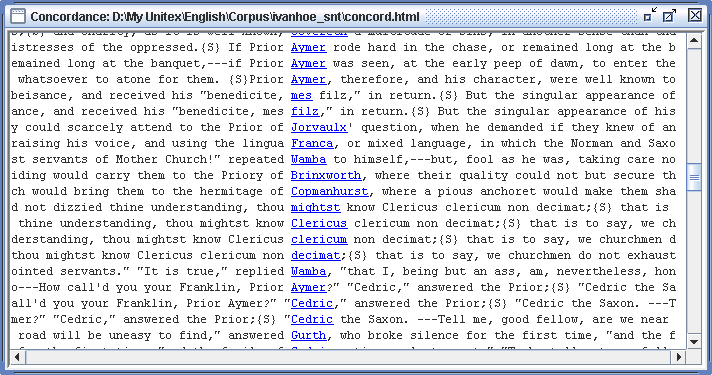
\includegraphics[width=15cm]{resources/img/fig4-1.png}
\caption{Result of the search for \texttt{<!DIC>}\label{fig-search-<!DIC>}}
\end{center}
\end{figure}

\bigskip
\noindent The negation of a dictionary mask like \verb+<V:G>+ will match any
word, except for those that are matched by this mask. For instance, \verb+<!V:G>+ will not
match the word \verb+being+, even if there are homonymic non-verbal entries in
the dictionaries:

\begin{verbatim}
being,.A
being,.N+Abst:s
being,.N+Hum:s
\end{verbatim}
\index{Words!unknown}

\noindent Here are some examples of lexical masks with the different types of constraints:

\begin{itemize}
  \item \verb$<A~Hum:fs>$: a non-human adjective in the feminine singular;
  \item \verb+<lire.V:P:F>+: the verb \textit{lire} in the present or future
  tense;
  \item \verb$<suis,suivre.V>$: the word \textit{suis} as inflected form of the
  verb \textit{suivre} (as opposed to the form of the verb \textit{\^etre});
  \item \verb$<facteur.N~Hum>$: all nominal entries that have \textit{facteur} as
  canonical form and that do not have the semantic code \verb+Hum+;
  \item \verb$<!ADV>$: all words that are not adverbs;
  \item \verb$<!WORD>$: all tokens that are not made of letters (cf.
  figure~\ref{fig-search-<!WORD>}). This mask does not recognize the sentence
  delimiter \verb+{S}+ and the special tag \verb+{STOP}+.
  \index{\verbt{\{S\}}}\index{Sentence delimiter}\index{\verbt{\{STOP\}}}
\end{itemize}

\bigskip
\begin{figure}[!ht]
\begin{center}
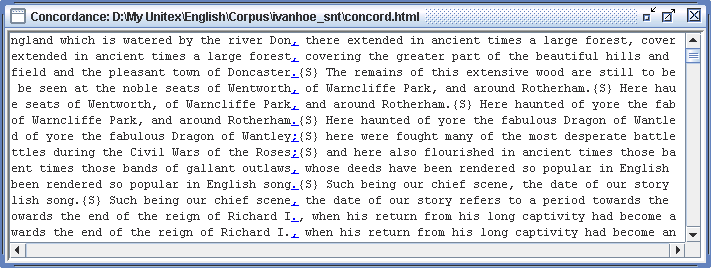
\includegraphics[width=15cm]{resources/img/fig4-2.png}
\caption{Result of a search for the pattern
\texttt{<!WORD>}\label{fig-search-<!WORD>}}
\end{center}
\end{figure}

\section{Concatenation}
\index{Concatenation of regular expressions}\index{\verbc{.}}
There are three ways to concatenate regular expressions. The first consists in
using the concatenation operator which is represented by the dot.
\index{Operator!concatenation}
Thus, the expression:

\begin{verbatim}
<DET>.<N>
\end{verbatim}

\noindent recognizes a determiner followed by a noun. The space can also be used for
concatenation, as well as the empty string. The following expressions:

\begin{verbatim}
the <A> cat
the<A>cat
\end{verbatim}

\noindent recognizes the token \textit{the}, followed by an adjective and the
token \textit{cat}. The parenthesis
\index{Parenthesis} are used as delimiters of a regular expression.  All of the
following expressions are equivalent:

\begin{verbatim}
the <A> cat
(the <A>)cat
the.<A>cat
(the).<A> cat
(the.(<A>)) (cat)
\end{verbatim}

\section{Union}
\index{Union of regular expressions}\index{\verbc{+}}
\index{Operator!disjunction}
The union of regular expressions is expressed by typing the character \verb$+$
between them. The expression

\begin{verbatim}
(I+you+he+she+it+we+they)<V>
\end{verbatim}

\noindent
recognizes a pronoun followed by a verb. If an element in an
expression is optional, it is sufficient to use the union of this
element and the empty word epsilon. \index{\verbc{<E>}} Examples:

\bigskip
\noindent \verb$the (little+<E>) cat$ recognizes the sequences \textit{the cat}
and \textit{the little cat}

\smallskip
\noindent \verb$(<E>+Anglo-).(French+Indian)$ recognizes \textit{French}, \textit{Indian},
\textit{Anglo-French} and \textit{Anglo-Indian}

\section{Kleene star}
\index{Kleene star}\index{\verbc{*}}\index{Operator!Kleene star}\index{Operator!iteration}
The Kleene star, represented by the character \verb+*+,  allows you to recognize
zero, one or several occurrences of an expression. The star must be placed on
the right hand side of the element in question. The expression:

\begin{verbatim}
this is very* cold
\end{verbatim}

\noindent recognizes \textit{this is cold}, \textit{this is very cold},
\textit{this is very very cold}, etc. The star has a higher priority than the
other operators. You have to use brackets in order to apply the star to a complex
expression. The expression:


\begin{verbatim}
0,(0+1+2+3+4+5+6+7+8+9)*
\end{verbatim}

\noindent recognizes a zero followed by a comma and by a possibly empty sequence of
digits.

\bigskip
\noindent WARNING: It is prohibited to search for the empty word with a regular
expression. If you try to search for \verb$(0+1+2+3+4+5+6+7+8+9)*$, the program
will raise an error as shown in
figure~\ref{fig-epsilon-error}.


\bigskip
\begin{figure}[!ht]
\begin{center}
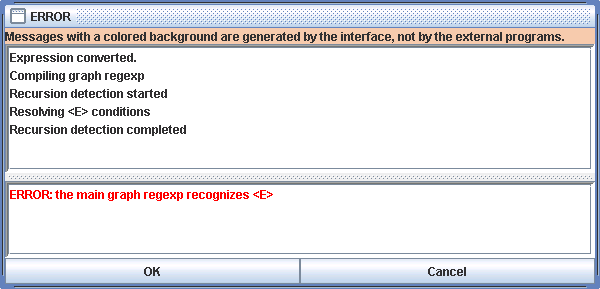
\includegraphics[width=14cm]{resources/img/fig4-3.png}
\caption{Error message when searching for the empty
string\label{fig-epsilon-error}}
\end{center}
\end{figure}


\section{Morphological filters}
\label{section-filters}
\index{Morphological filters}

It is possible to apply morphological filters to the lexemes found. For that, it is necessary to
immediately follow the lexeme found by a filter in double angle brackets:

\bigskip
\noindent
\textit{lexical mask}\verb$<<$\textit{morphological pattern}\verb$>>$ \\


\bigskip\index{Regular expressions}\index{POSIX}
\noindent The morphological filters are expressed as regular expressions in POSIX
format (see \cite{TRE} for the detailed syntax). Here are some examples of
elementary filters:



\begin{itemize}
  \item \verb$<<ss>>$: contains \verb$ss$
  \item \verb$<<^a>>$: begins with \verb$a$
  \item \verb+<<ez$>>+: ends with \verb$ez$
  \item \verb$<<a.s>>$: contains \verb$a$ followed by any character, followed by \verb$s$
  \item \verb$<<a.*s>>$: contains \verb$a$ followed by a sequence of any character, followed by \verb$s$
  \item \verb$<<ss|tt>>$: contains \verb$ss$ or \verb$tt$
  \item \verb$<<[aeiouy]>>$: contains a non accentuated vowel
  \item \verb$<<[aeiouy]{3,5}>>$: contains a sequence of non-accentuated vowels whose length 
        is between 3 and 5
  \item \verb$<<es?>>$: contains \verb$e$ followed by an
  optional \verb$s$
  \item \verb$<<ss[^e]?>>$: contains \verb$ss$ followed by an optional character which is not \verb$e$
\end{itemize}

\bigskip
\noindent It is possible to combine these elementary filters to form more complex filters:

\begin{itemize}
  \item \verb+<<[ai]ble$>>+: ends with \verb$able$ or \verb$ible$
  \item \verb$<<^(anti|pro)-?>>$: begins with \verb$anti$ or \verb$pro$, followed by an optional dash
  \item \verb+<<^([rst][aeiouy]){2,}$>>+: a word formed by 2 or more sequences beginning 
        with \verb$r$, \verb$s$
  or \verb$t$ followed by a non-accentuated vowel
  \item \verb!<<^([^l]|l[^e])>>!: does not begin with \verb$l$ unless the second letter is an
  \verb$e$, in other words, any word except the ones starting with \verb$le$. Such constraints
  are better described using contexts (see section~\ref{section-contexts}).
\end{itemize}

\noindent By default, a morphological filter alone is regarded as applying it to the lexical
mask \verb$<TOKEN>$, that means any token except space and \verb+{STOP}+. On the other hand,
when a filter follows a lexical mask immediately, it applies to what was recognized by the lexical
mask. Here are some examples of such combinations:

\begin{itemize}
  \item \verb+<V:K><<i$>>+: Past participle ending with \verb$i$
  \item \verb!<CDIC><<->>!: A compound word containing a dash
  \item \verb!<CDIC><< .* >>!: a compound word containing at least two spaces
  \item \verb!<A:fs><<^pro>>!: a feminine singular adjective beginning with \verb$pro$
  \item \verb!<DET><<^([^u]|(u[^n])|(un.+))>>!: a (French) determiner different from \verb$un$
  \item \verb+<!DIC><<es$>>+: a word which is not in the dictionary and which ends with \verb$es$
  \item \verb!<V:S:T><<uiss>>!: a verb in the past or present subjunctive, and containing \verb$uiss$
\end{itemize}

\noindent \index{Case sensitivity}NOTE: By default, morphological filters are
subject to the same variations of case as lexical masks. Thus, the filter
\verb$<<^b>>$ will recognize all the words starting with
\texttt{b}, but also those which start with \texttt{B}. 
To force the matcher to respect case, add \verb+_f_+ immediately
after the filter, \textit{e.g.}: \verb+<<^b>>_f_+.



\section{Search}
\index{Search for patterns}
\subsection{Search configuration}
\label{section-search-configuration}
In order to search for an expression, first open a text (cf.
chapter~\ref{chap-text}). Then click on "Locate Pattern..." in the "Text" menu.
The window of
figure~\ref{fig-regexp-search-configuration}
appears.

\bigskip
\begin{figure}[!ht]
\begin{center}
\includegraphics[width=8.8cm]{resources/img/fig4-4.png}
\caption{``Locate pattern'' window\label{fig-regexp-search-configuration}}
\end{center}
\end{figure}

\noindent The "Locate pattern in the form of" box allows you to select regular
expression or grammar. Click on "Regular expression".

\bigskip
\noindent The "Index" box allows you to select the recognition mode:

\bigskip
\index{Shortest matches}\index{Longest matches}\index{All matches}
\begin{itemize}
  \item "Shortest matches" : prefers shortest matches in case of nested
  sequences. For instance, if your grammar can recognize the sequences \textit{a very hot chili} and 
  \textit{very hot}, the first one will be discarded;
  \item "Longest matches" : prefers longest matches (\textit{a very hot chili}
  in our example). This is the default;
  \item "All matches" : outputs all recognized sequences.
\end{itemize}

\bigskip
\noindent The "Search limitation" box is used to  limit the number of results 
to a certain number of occurrences. By default, the search is limited to the first 200
occurrences.\index{Occurrences!number of}

\bigskip
\noindent The options of the "Grammar outputs" box do not concern regular
expressions. They are described in 
section~\ref{section-applying-graphs-to-text}. The same for options of tab
"Advanced options" (see section \ref{section-advanced-search-options}).

\bigskip
\noindent In the "Search algorithm" frame, you can specify wether you want to
perform the locate operation on the text using the \verb+Locate+ program or on
the text automaton with \verb+LocateTfst+. By default, search is done with the
\verb+Locate+ program, as Unitex always did until now. If you want to use
\verb+LocateTfst+, please read dedicated section \ref{section-locate-tfst}.

\bigskip
\noindent Enter an expression and click on "Search" in order to start the
search. Unitex will transform the expression into a grammar in the \verb+.grf+ format.
\index{File!\verbc{.grf}} This grammar will then be compiled into a grammar of
the \verb+.fst2+ format\index{File!\verbc{.fst2}} that will be used for the
search.

\subsection{Presentation of the results}
\label{section-display-occurrences}
When the search is finished, the window of
figure~\ref{fig-search-results} appears showing the number of matched
occurrences, the number of recognized tokens and the ratio between this 
number and the total number of tokens in the text.

\bigskip
\begin{figure}[!ht]
\begin{center}
\includegraphics[width=6.5cm]{resources/img/fig4-5.png}
\caption{Search results \label{fig-search-results}}
\end{center}
\end{figure}

\noindent After clicking on "OK" you will see
window~\ref{fig-configuration-concordance} appear, which allows you to configure
the presentation of the matched occurrences. You can also open this window by
clicking on "Located Sequences..." in the "Text" menu. The list of
occurrences is called a \textit{concordance}.\index{Concordance}


\bigskip
\begin{figure}[!ht]
\begin{center}
\includegraphics[width=11cm]{resources/img/fig4-6.png}
\caption{Result display configuration\label{fig-configuration-concordance}}
\end{center}
\end{figure}

\bigskip
\noindent The "Modify text" box offers the possibility to replace the matched
occurrences with the generated outputs. This possibility will be examined in 
chapter~\ref{chap-advanced-grammars}.

\bigskip
\noindent The "Extract units" box allows you to create a text file with all
the sentences that do or do not contain matched units. With the button "Set File",
you can select the output file. Then click on "Extract matching units" or
"Extract unmatching units" depending on whether you are interested in sentences
with or without matching units.

\bigskip
\noindent In the "Show matching sequences in context" box, you can select the
length in characters of the left and right contexts of the occurrences that will be
presented in the concordance. If an occurrence has less characters than its
right context, the line will be completed with the necessary number of
characters. If an occurrence has a length greater than that of the right
context, it will be displayed completely.

\bigskip
\noindent NOTE: in Thai, the size of the contexts is measured in displayable
characters and not in real characters. This makes it possible to keep the line alignment in
the concordance despite the presence of diacritics that combine with other
letters instead of being displayed as normal characters.

\index{Sorting!concordances}
\index{Contexts!concordance}
\bigskip
\noindent You can choose the sort order in the list "Sort According to". The
mode "Text Order" displays the occurrences in the order of their appearance in the text. The other six
modes allow you to sort in columns. The three zones of a line are the left
context, the occurrence and the right context. The occurrences and the right
contexts are sorted from left to right. The left contexts are sorted from right
to left. The default mode is "Center, Left Col.". The concordance is generated
in the form of an HTML file.\index{File!HTML}

\bigskip
\noindent If a concordance reaches several thousands of occurrences, it is advisable to
display it  in a web browser (Firefox \cite{Firefox}, Netscape \cite{Netscape},
Internet Explorer, etc.) instead.\index{Web browser} Check "Use a web
browser to view the concordance" (cf. figure~\ref{fig-configuration-concordance}). 
This option is activated by default if the number of occurrences is greater than 2000.
You can configure which web browser to use by clicking on "Preferences..." in
the menu "Info". Click on the tab "Language \& Presentation" and
select the program to use in the field "Html Viewer" 
(cf. figure~\ref{fig-browser-selection}).

\bigskip
\noindent \index{Concordance!frame} If you choose to open the concordance in
Unitex, you will see a window as shown on Figure \ref{fig-example-concordance}. 
Occurrences react as hyperlinks. If you click on an occurrence, the text frame is
opened and the corresponding sequence is highlighted. Moreover, if the text automaton is
available and if this window is not iconified, the sentence automaton that
contains the occurrence will be shown. 

\bigskip
\begin{figure}[!ht]
\begin{center}
\includegraphics[width=8cm]{resources/img/fig4-7.png}
\caption{Selection of a web browser for displaying
concordances\label{fig-browser-selection}}
\end{center}
\end{figure}

\bigskip
\begin{figure}[!p]
\begin{center}
\includegraphics[height=18cm]{resources/img/fig4-8.png}
\caption{Example concordance\label{fig-example-concordance}}
\end{center}
\end{figure}

\clearpage
\subsection{Statistics}
\label{section-statistics}
If you select the ``Statistics'' tab in the ``Located sequences..''
frame, you will see the panel shown on figure~\ref{fig-statistics}. This panel
allows you to get some statistics from the previously indexed sequences. 

\bigskip
\begin{figure}[!ht]
\begin{center}
\includegraphics[width=11cm]{resources/img/fig4-9.png}
\caption{Statistics panel\label{fig-statistics}}
\end{center}
\end{figure}

\bigskip
\noindent In the ``Mode'' panel, you can select the kind of statistics you want:
\begin{itemize}
  \item collocates by z-score: the previous one, plus some additionnal
  information (number of occurrences of the collocate in the match context and
  in the whole corpus, z-score of the collocate)
  \item collocates by frequency: shows the tokens that cooccur in the match
  context
  \item contexts by frequency: shows matches with left and right contexts (see
  below). ``count'' is the number of occurrences of a given match+context
\end{itemize}

\bigskip
\noindent In the second panel, you can set the lenght of left and right
contexts to be used, in non space tokens. NOTE: this notion of context has
nothing to do with contexts in grammars.

\bigskip
\noindent In the last panel, you can allow or not case variations. If you allow
case variations, \verb$the$ and \verb$THE$ will be considered as a same token,
and the count will be the sum of the counts of \verb$the$ and \verb$THE$.

\bigskip
\noindent The following figures show the statistics computed in each mode for
the query \verb$<have>$ on \verb$ivanhoe.snt$.


\bigskip
\begin{figure}[!ht]
\begin{center}
\includegraphics[width=11cm]{resources/img/fig4-10.png}
\caption{left+match+right count\label{fig-statistics-mode0}}
\end{center}
\end{figure}

\begin{figure}[!ht]
\begin{center}
\includegraphics[width=11cm]{resources/img/fig4-11.png}
\caption{collocate count\label{fig-statistics-mode1}}
\end{center}
\end{figure}

\begin{figure}[!ht]
\begin{center}
\includegraphics[width=12cm]{resources/img/fig4-12.png}
\caption{collocate, count and other information\label{fig-statistics-mode2}}
\end{center}
\end{figure}

\chapter{Local grammars}
\label{chap-grammars}

Local grammars are a powerful tool to represent the majority of linguistic
phenomena. The first section presents the formalism in which these grammars are
represented. Then we will see how to construct and present grammars using Unitex.

\section{The local grammar formalism}
\index{Grammars!formalism}

\subsection{Algebraic grammars}
Unitex grammars are variants of algebraic grammars, also known as context-free
grammars. \index{Grammars!context-free} An algebraic grammar consists of
rewriting rules. Below you see a grammar that matches any number of $a$
characters:

\bigskip $S \rightarrow$ $aS$

$S \rightarrow$ \E

\bigskip
\noindent The symbols to the left of the rules are called \textit{non-terminal
symbols}\index{Symbols!non-terminal}\index{Non-terminal symbols}  since they can
be replaced. Symbols that cannot be replaced by other rules are called
\textit{terminal symbols}\index{Symbols!terminal}. The items at the right side
are sequences of non-terminal and terminal symbols. The epsilon symbol \E ~
designates the empty word. In the grammar above, $S$ is a non-terminal symbol and
$a$ a terminal (symbol). $S$ can be rewritten as either an $a$ followed by a $S$
or as the empty word. The operation of rewriting by applying a rule is called
\textit{derivation}.\index{Derivation} We say that a grammar generates a word if
there exists a sequence of derivations that produces that word. The non-terminal
that is the starting point of the first derivation is called an
\textit{axiom}.\index{Axiom}\index{Rules!rewriting}


\bigskip
\noindent The grammar above also generates the word \textit{aa}, since we can
derive this word according to the axiom $S$ by applying the following derivations:

\bigskip Derivation 1: rewriting the axiom to $aS$

\underline{$S$} $\rightarrow aS$

\bigskip Derivation 2: rewriting $S$ at the right side of $aS$

$S$ $\rightarrow a$\underline{$S$} $\rightarrow aaS$

\bigskip Derivation 3: rewriting $S$ to \E

$S$ $\rightarrow aS \rightarrow aa$\underline{$S$} $\rightarrow aa$

\bigskip
\noindent We call the set of words generated by a grammar the \textit{language
generated by the grammar}. The languages generated by algebraic grammars are
called \textit{algebraic languages}\index{Algebraic languages} or
\textit{context-free languages}\index{Context-free languages}.


\subsection{Extended algebraic grammars}
\index{Grammars!extended algebraic}

Extended algebraic grammars are algebraic grammars where the members on the right
side of the rule are not just sequences of symbols but regular
expressions.\index{Regular expressions} Thus, the grammar that generates a
sequence of an arbitrary number of $a$'s can be written as a grammar consisting
of one rule:

\bigskip $S \rightarrow$ $a^{*}$

\bigskip
\noindent These grammars, also called \textit{recursive transition networks}
(\textit{RTN})\index{Recursive Transition Networks}\index{RTN} or \textit{syntax
diagrams}\index{Syntax diagrams}, are suited for a user-friendly graphical
representation. Indeed, the right member of a rule can be represented as a graph
whose name is the left member of the rule.

\bigskip
\noindent However, Unitex grammars are not exactly extended algebraic grammars, since they
contain the notion of \textit{transduction}.\index{Transduction} This notion,
which is derived from the field of finite state automata, enables a grammar to
produce some output. With an eye towards clarity, we will use the terms grammar
or graph. When a grammar produces outputs, we will use the term
\textit{transducer},\index{Transducer} as an extension of the definition of a
transducer in the area of finite state automata.\index{Automata!finite state}


\section{Editing graphs}
\label{section-editing-graphs}
\subsection{Creating a graph}
In order to create a graph, click on "New" in the "FSGraph" menu. You will then
see the window coming up as in figure~\ref{fig-new-graph}. The symbol in
arrow form is the \textit{initial state} of the graph.\index{State!initial} The
round symbol with a square is the \textit{final state} of the
graph.\index{State!final} The grammar only recognizes expressions that are
described along the paths between initial and final states.

\begin{figure}[!h]
\begin{center}
\includegraphics[width=13cm]{resources/img/fig5-1.png}
\caption{FSGraph menu}
\end{center}
\end{figure}

\begin{figure}[!h]
\begin{center}
\includegraphics[width=14.5cm]{resources/img/fig5-2.png}
\caption{Empty graph\label{fig-new-graph}}
\end{center}
\end{figure}

\bigskip
\noindent In order to create a box, click inside the window while pressing the Ctrl
key.\index{Graph!creating a box}\index{Creating a Box}\index{Boxes!creating}
A blue rectangle will appear that symbolizes the empty box that was created (see
figure~\ref{fig-box-creation}). After creating the box, it is automatically selected. 


\noindent If you use Unitex on a Macintosh device, you must press the "Command key" 
instead of Ctrl in every action involving the Ctrl key.

\bigskip
\noindent You see the contents of that box in the text field at the top of the
window. The newly created box contains the \verb+<E>+ symbol that represents the empty word
epsilon.\index{\verb+<E>+} Replace this symbol by the text \verb$I+you+he+she+it+we+they$ and
press the Enter key. You see that the box now contains seven lines (see
figure~\ref{fig-pronoun-box}). The \verb$+$ character serves as a
separator.\index{\verb$+$} The box is displayed in the form of red text lines since it is 
not connected to another one at the moment.
We often use this type of boxes to insert comments into a
graph. \index{Graph!comments in}\index{Comments!in a graph}

\bigskip
\noindent If you intend to insert comments into a graph, you can create a box starting with \verb$/$.
The text in this box will be displayed in green, and may contain empty lines.
This box can't have any incoming nor outgoing transitions (see
figure~\ref{comment-box}).

\begin{figure}[!hb]
\begin{center}
\includegraphics[width=14.5cm]{resources/img/fig5-3.png}
\caption{Creating a box\label{fig-box-creation}}
\end{center}
\end{figure}

\begin{figure}[!hb]
\begin{center}
\includegraphics[width=14.5cm]{resources/img/fig5-4.png}
\caption{Box containing
\texttt{I+you+he+she+it+we+they}\label{fig-pronoun-box}}
\end{center}
\end{figure}

\begin{figure}[!h]
\begin{center}
\includegraphics[width=12.5cm]{resources/img/fig5-4b.png}
\caption{Box containing comments\label{comment-box}}
\end{center}
\end{figure}
%\clearpage

\bigskip
\noindent To connect a box to another one, first click on the source box, then
click on the target box.\index{Graph!connecting boxes}\index{Boxes!connecting} If there
already exists a transition between two boxes, it is deleted. It is also possible
to do that by clicking first on the target box and then on the
source box while pressing Shift. In our example, after connecting the box to the initial
and final states of the graph, we get a graph as in
figure~\ref{fig-pronoun-graph}:

\begin{figure}[!ht]
\begin{center}
\includegraphics[width=12.5cm]{resources/img/fig5-5.png}
\caption{Graph that recognizes English
pronouns\label{fig-pronoun-graph}}
\end{center}
\end{figure}
\pagebreak
\bigskip
\noindent NOTE: If you double-click a box, you connect this box to itself (see
figure~\ref{fig-loop-box}). To undo this double-click on the
same box a second time, or use the "Undo" button.

\bigskip
\begin{figure}[!h]
\begin{center}
\includegraphics[width=4.5cm]{resources/img/fig5-6.png}
\caption{Box connected to itself\label{fig-loop-box}}
\end{center}
\end{figure}

\noindent Click on "Save as..." in the "FSGraph" menu to save the graph.
\index{Graph!saving} By default, Unitex proposes to save the graph in the
sub-directory \verb+Graphs+ in your personal folder. You can see if the 
graph was modified after the last
saving by checking if the title contains the text \verb+(Unsaved)+.

\bigskip
\noindent When editing a graph you can bring up a specific contextual menu to 
perform standard graph edition operations by right clicking in the background of the graph window.
This menu will offer several operations that are frequently used when editing a graph.
\begin{itemize}
\item create a new box
\item save, print the current graph or set up the page parameters
\item the usual "Tools", "Format" and "Zoom" menu also accessible in the FSGraph menu 
\end{itemize}
If one or several boxes are currently selected, the following menus will be accessible, allowing you to apply specific operations to these sets of boxes. Otherwise, these menus are useless and therefore non accessible. 
\begin{itemize}
\item surround selected boxes with an input or output variable definition, with contexts, or with Morphological mode delimiters. These operations are also accessible via the Toolbar of the graph edition window (see section~\ref{toolbar-commands}). 
\item merge selected boxes
\item export as a new graph
\end{itemize}
\bigskip
\begin{figure}[!h]
\begin{center}
\includegraphics[width=7.5cm]{resources/img/fig5-6b.png}
\caption{contextual menu\label{contextual-menu}}
\end{center}
\end{figure}

\subsection{Sub-Graphs}
\label{section-subgraphs}
\index{Graph!calling a sub-graph}\index{\verb+:+}
In order to call a sub-graph, its name is inserted into a box and preceded by the
\verb+:+ character. If you enter the text:

\bigskip
\verb$alpha+:beta+gamma+:E:\greek\delta.grf$

\bigskip
\noindent into a box, you get a box similar to the one in
figure~\ref{fig-subgraph-call}:

\medskip
\begin{figure}[h]
\begin{center}
\includegraphics[width=6cm]{resources/img/fig5-7.png}
\caption{Graph that calls sub-graphs \texttt{beta} and
\texttt{delta}\label{fig-subgraph-call}}
\end{center}
\end{figure}

\noindent You can indicate the full name of the graph
(\verb$E:\greek\delta.grf$) or simply the base name without the path (\verb$beta$); 
in this case, the sub-graph is expected to be in the same directory as the graph that references
it. References to absolute path names should as a rule be avoided, since such
calls are not portable. If you use such an absolute path name, the graph compiler
will emit a warning (see figure~\ref{fig-warning-absolute-graph-name}).

\begin{figure}[!h]
\begin{center}
\includegraphics[width=14.5cm]{resources/img/fig5-8.png}
\caption{Warning about a non portable graph
name\label{fig-warning-absolute-graph-name}}
\end{center}
\end{figure}


\bigskip
\noindent For portability you should not use \verb+\+ or \verb+/+ as separator
in graph path names. Use instead \verb+:+ which is understood as a
system-independent separator. In figure~\ref{fig-warning-absolute-graph-name}
\verb+\+ and \verb+/+ are internally converted by the graph compiler to \verb+:+
(\verb+E::greek:delta.grf+).


%\clearpage
%\bigskip

\bigskip
\noindent \textbf{Graph repository}
\label{section-repository}

\bigskip
\noindent When you need to call a grammar $X$ inside a grammar $Y$, a simple
method is to copy all the graphs of $X$ into the directory that contains the
graphs of $Y$. This method raises two problems:

\begin{itemize}
  \item the number of graphs in the directory grows quickly;
  \item two graphs cannot share the same name.
\end{itemize}

\noindent To avoid that, you can store the grammar $X$ in a special directory,
called the \textit{graph repository}.\index{Graph!repository} This directory is a
kind of library where you can store graphs, and then call them using \verb+::+
instead of \verb+:+. To use this mechanism, you first need to set the path to the
graph repository. Go into the "Info>Preferences...>Directories" menu, and select
your directory in the "Graph repository" frame (see Figure \ref{directories}).
There is one graph repository per language, so feel free to share or not the same
directory for all the languages you work with.

\begin{figure}[!h]
\begin{center}
\includegraphics[width=8cm]{resources/img/fig5-10.png}
\caption{Setting the path to the graph repository\label{directories}}
\end{center}
\end{figure}

%\clearpage

\bigskip
\noindent Let us assume that we have a repository tree as on Figure
\ref{repository}. If we want to call the graph named \verb+DET+ that is located
in sub-directory \verb+Johnson+, we must use the call

% do not remove this line jump
\noindent \verb+::Det:Johnson:DET+
(see Figure \ref{repository-graph-call}\,\footnote{To avoid confusion, graph calls
that refer to the repository are displayed in brown instead of grey.}).


\bigskip
\begin{figure}[!h]
\begin{center}
\includegraphics[width=3.9cm]{resources/img/fig5-11.png}
\caption{Graph repository example\label{repository}}
\end{center}
\end{figure}

\begin{figure}[!h]
\begin{center}
\includegraphics[width=6.7cm]{resources/img/fig5-12.png}
\caption{Call to a graph located in the
repository\label{repository-graph-call}}
\end{center}
\end{figure}

%\clearpage

\noindent TRICK: If you want to avoid long path names like
\verb+::Det:Johnson:DET+, you can create a graph named \verb+DET+ and put it the
repository root (here \verb+D:\repository\DET.grf+). In this graph, just put a
call to \verb+::Det:Johnson:DET+. Then, you can just call \verb+::DET+ in your
own graphs. This has two advantages: 1) you do not have long path names; 2) you
can modify the graphs in your repository with no constraint on your own graphs,
because the only graph that will have to be modified is the one located at the
repository root.

\begin{figure}[h!]
\begin{center}
\includegraphics[width=7cm]{resources/img/fig5-9.png}
\caption{Missing called sub-graphs appear in red\label{call-colours}}
\end{center}
\end{figure}


\bigskip
\noindent Calls to sub-graphs are represented in the boxes by grey lines, as in Fig.~\ref{call-colours}, or brown
lines in the case of graphs located in the repository, as in Fig.~\ref{repository-graph-call}. If the .GRF File of the sub-graph is not found at the path you indicated, Unitex will try to find a fst2 file of the same name. If Unitex can't find any of the .grf and .fst2 files, the call to the missing subgraph will be displayed on a red line. 
On Windows, you can open a sub-graph by clicking on the grey line while pressing the Alt key.
On Linux, the <Alt+Click>  combination is intercepted by the system:\footnote{If you are 
working on KDE, you can deactivate <Alt+Click> in kcontrol.} in order to open a
sub-graph, middle-click on its name, or click on its name by pressing the left and the right mouse buttons
simultaneously.

\bigskip
\noindent The list of subgraphs called from the current graph and the graphs in which the current graph is called can be displayed by clicking on the second and third button of the fourth set of buttons in the toolbar command (see Figure~\ref{list-called-graphs} and
Figure~\ref{fig-toolbar} in section~\ref{toolbar-commands}).
In these Lists of subgraphs : 
\begin{itemize}
\item sub-graphs directly called from the current graph appear with their simple filename
\item sub-graphs indirectly called from one of the graphs called by the current graph appear with an arrow before their filename.
\item sub-graphs that appear in one of the graphs that are called from the current one but that are unplugged and never processed appear in orange
\item sub-graphs that are not found (neither .grf nor .fst2) appear in red
\end{itemize}

\begin{figure}[!h]
\begin{center}
\includegraphics[width=15.2cm]{resources/img/fig5-12b.png}
\caption{Display the list of all called graphs\label{list-called-graphs}}
\end{center}
\end{figure}

\subsection{Manipulating boxes}
\index{Multiple selection}\index{Boxes!selection}

You can select several boxes using the mouse. In order to do so, click and drag the
mouse without releasing the button. When you release the button, all boxes
touched by the selection rectangle will be selected and are displayed in
white on a blue background, as shown on Figure \ref{multi-selection}.

\begin{figure}[!ht]
\begin{center}
\includegraphics[width=10cm]{resources/img/fig5-13.png}
\caption{Selecting several boxes\label{multi-selection}}
\end{center}
\end{figure}
%\bigskip
\noindent You can select several boxes by keeping simultaneously the <CTRL> and <SHIFT> keys pressed and by clicking on every box you want to add to your current selection. This way you can select several boxes without selecting all the boxes located in their area.

\begin{figure}[!ht]
\begin{center}
\includegraphics[width=10cm]{resources/img/fig5-13b.png}
\caption{Selecting distant boxes\label{multi-selection}}
\end{center}
\end{figure}
\bigskip
\noindent When boxes are selected, you can move them by clicking and
dragging the cursor without releasing the button. In order to cancel the selection, click on
an empty area of the graph. If you click on a box, all the boxes of the selection
will be connected to it.

\bigskip
\index{Multiple selection!copy-paste}
\index{Copy}\index{Paste}
\noindent You can perform a copy-paste with several boxes. Select them and
press <Ctrl+C> or click on "Copy" in the "Edit" menu. The selection is now in the Unitex
clipboard. You can then paste this selection by pressing <Ctrl+V> or by selecting
"Paste" in the "Edit" menu.

\bigskip
\begin{figure}[!h]
\begin{center}
\includegraphics[width=13cm]{resources/img/fig5-14.png}
\caption{Copy-Paste of a multiple selection}
\end{center}
\end{figure}

\noindent NOTE: You can paste a multiple selection into a different graph from
the one where you copied it from.

\bigskip
\index{Graph!deleting boxes}\index{Boxes!deleting}
\noindent In order to delete boxes, select them, delete the text that they
contain (\textit{i.e.} the text presented in the text field above the window)
and press the Enter key.

\bigskip
\noindent The initial and final states cannot be deleted.

\subsection{Transducers}
\index{Transducers}\index{\verb+/+}
A transducer is a graph in which outputs can be associated with boxes. To insert
an output, use the special character \verb+/+. All characters to the right of
it will be part of the output. Thus, the text \verb$one+two+three/number$ results in
a box like in figure~\ref{fig-exemple-transduction}.

\begin{figure}[h]
\begin{center}
\includegraphics[width=4.5cm]{resources/img/fig5-15.png}
\caption{Example of a transducer\label{fig-exemple-transduction}}
\end{center}
\end{figure}

\noindent To create an empty box with an output consisting of \verb+number+, type \verb+<E>/number+ (example: the rightmost box in Fig.~\ref{fig-using-variable} is empty and has an output). The output associated with a box is represented in bold text below it.

\subsubsection{Weights}

You can assign integer weights to the boxes of a transducer.
Thus, when a sequence of tokens is matched by several paths, 
only the one with the highest weight will produce an output. 
After a locate, this will affect the concordance, in which 
the matched sequences of words will appear only once with the appropriate output
(Figure~\ref{fig-weights-in-graphs}). In order to assign weight 1 to a box, insert \verb+${1}$+
in the output of the box, e.g. as in \verb+<E>/${1}$+. The weight of a path is the sum of the weights found in the path.

\bigskip
\noindent With weights, you can define a priority among paths that match the same sequence.
You cannot define a priority among embedded matching sequences (cf. section~\ref{section-search-configuration})
 or among overlapping matching sequences (cf. section~\ref{section-priority-leftmost-match}).

\bigskip
\begin{figure}[h!]
\begin{center}
\includegraphics[width=14.5cm]{resources/img/fig5-15b.png}
\caption{weights in graphs \label{fig-weights-in-graphs}}
\end{center}
\end{figure}

\subsection{Input Variables}
\label{section-using-variables}
\index{Graph!variables in a}\index{Variables!input}\index{\verb+$+}
\index{Transducer!with variables}

It is possible to select parts of a text sequence recognized by a grammar using input
variables. To associate an input variable \verb+var1+ with parts of a grammar, use the special
symbols \verb+$var1(+ and \verb+$var1)+ to define the beginning and the end of
the part to be stored. Create two boxes containing one \verb+$var1(+ and the second
\verb+$var1)+. These boxes must not contain anything but the variable name
preceded by \verb+$+ and followed by a parenthesis. Then link these boxes to the
zone of the grammar to be stored. The graph in
figure~\ref{fig-using-variable} recognises a sequence of digits before
\verb+dollar+ or \verb+dollars+. This sequence will be stored in a variable named
\verb+var1+.

\bigskip
\begin{figure}[h]
\begin{center}
\includegraphics[width=13.5cm]{resources/img/fig5-16.png}
\caption{Using the input variable
\texttt{var1}\label{fig-using-variable}}
\end{center}
\end{figure}

\noindent Variable names may contain latin letters (without accents), upper or
lower case, numbers, or the \verb+_+ (underscore) character.\index{\verb+_+}\index{Variable
names} Unitex distinguishes between uppercase and lowercase characters.
\index{Underscore}

\bigskip
\noindent Once a variable is defined, you can use it in transducer outputs by
surrounding its name with \verb+$+.\index{\verb+$+} The grammar in
figure~\ref{fig-date-grammar} recognizes a date formed by a month and a
year, and produces the same date as an output, but in the order year-month.

\bigskip
\begin{figure}[h]
\begin{center}
\includegraphics[width=14.5cm]{resources/img/fig5-17.png}
\caption{Inverting month and year in a date\label{fig-date-grammar}}
\end{center}
\end{figure}

\noindent If you want to use the character \verb+$+ in the output of a box, you
have to double it, as shown on figure~\ref{fig-using-variable}.

\bigskip
\noindent The default behavior of \verb+Locate+ and \verb+LocateTfst+ is to
consider variables that have not been defined as being empty. You can
modify this behavior as shown in section \ref{section-advanced-search-options}.
Moreover, it is possible to test whether a variable has been defined or not, as
shown in section \ref{section-variables}.

\subsection{Copying lists}
\index{Copying lists}
\index{Copy}\index{Paste}

It can be practical to perform a copy-paste operation on a list of words or
expressions from a text editor to a box in a graph. In order to avoid having to
copy every term manually, Unitex provides a mean to copy lists. To use this,
select the list in your text editor and copy it using <Ctrl+C> or the copy
function integrated in your editor. Then create a box in your graph, and press
<Ctrl+V> or use the "Paste" command in the "Edit" menu to paste it into the box.
A window as in Figure~\ref{fig-setting-contexts-for-multiple-copy}
opens:

\bigskip
\begin{figure}[h]
\begin{center}
\includegraphics[width=7cm]{resources/img/fig5-18.png}
\caption{Selecting a context for copying a list\label{fig-setting-contexts-for-multiple-copy}}
\end{center}
\end{figure}
\index{Contexts!copy of a list}

\noindent This window allows you to define the left and right contexts that will
automatically be used for each term of the list. By default, these contexts are
empty. If you use the contexts  \verb+<+ and \verb+.V>+ with the following list:

\bigskip
\textit{eat}

\textit{sleep}

\textit{drink}

\textit{play}

\textit{read}

\bigskip
\noindent you will get the box in figure~\ref{fig-multiple-copy}:

\bigskip
\begin{figure}[h]
\begin{center}
\includegraphics[width=6.7cm]{resources/img/fig5-19.png}
\caption{Box resulting from copying a list and applying contexts\label{fig-multiple-copy}}
\end{center}
\end{figure}

\subsection{Special Symbols}
\index{Symbols!special}
\noindent The Unitex graph editor interprets the following symbol in a special manner:

\bigskip
\verb," + : / < > # \,

\bigskip
\noindent Table~\ref{tab-special-symbols} summarizes the meaning of
these symbols for Unitex, as well as the ways to recognize these characters in texts.

\bigskip
\index{Meta-characters}
\begin{table}[h]
\begin{center}
\begin{tabular}{|c|p{9cm}|c|}
\hline
\texttt{Caracter} & \texttt{Meaning} & \texttt{Escape}
\\
\hline \verb$"$ & quotation marks mark sequences that must not be interpreted by
Unitex, and whose case must be taken verbatim & \verb$\"$
\\
\hline
\verb$+$ & \verb$+$ separates different lines within the boxes& \verb$"+"$
\\
\hline
\verb$:$ & \verb$:$ introduces a call to a subgraph& \verb$":"$ or \verb$\:$
\\
\hline
\verb$/$ & \verb$/$ indicates the start of a transduction within a box& \verb$\/$
\\
\hline
\verb$<$ & \verb$<$ indicates the start of a pattern or a meta & \verb$"<"$ or \verb$\<$
\\
\hline
\verb$>$ & \verb$>$ indicates the end of a pattern or a meta& \verb$">"$ or \verb$\>$
\\
\hline
\verb$#$ & \verb$#$ prohibits the presence of a space& \verb$"#"$
\\
\hline
\verb$\$ & \verb$\$ escapes most of the special characters & \verb$\\$
\\
\hline
\end{tabular}
\caption{Encoding of special characters in the graph
editor\label{tab-special-symbols}}
\end{center}
\end{table}

\subsection{Toolbar Commands}
\index{Toolbar}
\label{toolbar-commands}

The toolbar above a graph contains shortcuts for certain commands
and allows you to manipulate boxes of a graph by using some "tools". This
toolbar may be moved by clicking on the "rough" zone. It may also be dissociated
from the graph and appear in an separate window (see
figure~\ref{fig-toolbar}). In this case, closing this window puts
the toolbar back at its initial position. Each graph has its own toolbar.

\begin{figure}[!ht]
\begin{center}
\includegraphics[width=15.6cm]{resources/img/fig5-20.png}
\caption{Toolbar\label{fig-toolbar}}
\end{center}
\end{figure}

%\bigskip
\medskip
\index{Copy}\index{Cut}\index{Paste}
\noindent The first two icons are shortcuts for saving and compiling the graph.
The following five correspond to the Copy, Cut, Paste, Redo and Undo operations. 

\bigskip
\noindent The following six icons correspond to edit commands for boxes. The first
one, a white arrow, corresponds to the boxes' normal edit mode. The next 5 icons
correspond to specific tools. In order to use a tool, click on the
corresponding icon: the mouse cursor changes its form and mouse clicks are then
interpreted in a particular fashion. What follows is a description of these
tools, from left to right:

\begin{itemize}
  \item creating boxes: creates a box at the empty place where the mouse was clicked;
  \item deleting boxes: deletes the box that you click on;
  \item connect boxes to another box: using this utility you select one or
  more boxes and connect it or them to another one. In contrast to the
  normal mode, the connections are inserted to the box where the mouse button
  was released on;
  \item connect boxes to another box in the opposite direction: this utility
  performs the same operation as the one described above, but connects the boxes
  to the one clicked on in opposite direction;
  \item open a sub-graph: opens a sub-graph when you click on a grey line within a box.
\end{itemize}
In order to change the cursor back to its normal form, the white arrow, right-click on the background of the graph:
then, mouse clicks will be interpreted in the normal way again.

\bigskip
\noindent The next icon (showing a wrench) is a shortcut to open the window with the graph display
options.
%%%%%%%%%%%%%%%%%%%%%%%%%%%%%%%%%%%%%%%%%
The following two icons allow you to view lists of graphs that are related to the current graph by a  "graph/subgraph" relation :
\begin{itemize}
\item The first displays a list of graphs called by the current graph
\item The second button shows the list of all the graphs calling the current graph as a subgraph.
\end{itemize}
The two green arrows button will refresh the current graph to load the latest version of the current graph. If any graph has its .grf file changed by any operation while displayed in a Unitex window, a window will pop up to warn you and invite you to refresh its window.

\bigskip
\noindent The balance button allows you to compare the current graph to another graph or another version of the same graph. This will display a new window (as in Figure~\ref{Graph-DIFF}) containing both graphs with colours pointing out the different types of changes between the two graphs: insertion, removal, moves of each state of the graph and change of the content of a state (respectively in green, red, purple and yellow).

\bigskip
\noindent 
\begin{figure}[!h]
\begin{center}
\includegraphics[width=15.6cm]{resources/img/DIFF.png}
\caption{DIFF\label{Graph-DIFF}}
\end{center}
\end{figure}
\bigskip
\noindent 

The last six buttons are shortcuts to use variables, morphological mode or insert contexts around one or several selected states. These buttons will be clickable only when one or several states are currently selected :
\begin{itemize}
\item \textcolor{red}{()}  : input variable	(see section~\ref{section-using-variables})
\item \textcolor{blue}{()} : output variable (see section~\ref{section-output-variables})
\item \textcolor{magenta}{<>}  : morphological mode (see section~\ref{section-morphological-mode})
\item \textcolor{green}{\$*} : left context (see section~\ref{section-contexts})
\item \textcolor{green}{\$[} : right context (see section~\ref{section-contexts})
\item \textcolor{green}{\$![} : negative right context (see section~\ref{section-contexts})
\end{itemize}

\bigskip
%\pagebreak
%%%%%%%%%%%%%%%%%%%%%%%%%%%%%%%%%%%%%%%%%
%%%%%%%%%%%%%%%%%%%%%%%%%%%%%%%%%%%%%%%%%
\section{Display options}
\index{Graph!display}

\subsection{Sorting the lines of a box}
\index{Sorting!lines of a box}\index{Boxes!sorting lines}
You can sort the content of a box by selecting it and clicking on "Sort Node
Label" in the "Tools" submenu of the "FSGraph" menu. This sort operation does
not use the \verb+SortTxt+ program. It uses a basic sort mechanism that sorts
the lines of the box according to the order of the characters in the Unicode
encoding.
\index{Unicode}

\begin{figure}[!h]
\begin{center}
\includegraphics[width=6cm]{resources/img/fig5-21.png}
\caption{Zoom sub-menu}
\end{center}
\end{figure}
\subsection{Zoom}
\index{Zoom}\index{Graph!zoom}
The "Zoom" submenu allows you to choose the zoom scale that is applied to display the graph.
%\bigskip
\noindent The "Fit in screen" option stretches or shrinks the graph in order to fit it into the screen. The "Fit in window" option adjusts the graph so that it is displayed entirely in the window.

\clearpage
\subsection{Antialiasing}
\index{Antialiasing}\index{Graph!antialiasing}
Antialiasing is a shading effect that avoids pixelization
effects.\index{Pixellisation} You can activate this effect by clicking on
"Antialiasing..." in the "Format" sub-menu. Figure~\ref{fig-antialiasing}
shows one graph displayed normally (the graph on top) and with antialiasing (the
graph at the bottom).

\bigskip
\begin{figure}[!ht]
\begin{center}
\includegraphics[width=13.5cm]{resources/img/fig5-22.png}
\caption{Antialiasing example\label{fig-antialiasing}}
\end{center}
\end{figure}

\noindent This effect slows Unitex down. We recommend  not to use it if your
machine is not powerful enough.

\clearpage 
\subsection{Box alignment}\index{Boxes!alignement}
\index{Box alignement}\index{Graph!box alignment}

In order to get nice-looking graphs, it is useful to align the boxes, both
horizontally and  vertically. To do this, select the boxes to align and click on
"Alignment..." in the "Format" sub-menu of the "FSGraph" menu or press <Ctrl+M>.
You will then see the window in Figure~\ref{fig-alignment-frame}.

\bigskip
\noindent The possibilities for horizontal alignment are:
\begin{itemize}
  \item Top: boxes are aligned with  the top-most box;
  \item Center: boxes are centered on the same axis;
  \item Bottom: boxes are aligned with the bottom-most box.
\end{itemize}

\begin{figure}[!h]
\begin{center}
\includegraphics[width=6.6cm]{resources/img/fig5-23.png}
\caption{Alignment window\label{fig-alignment-frame}}
\end{center}
\end{figure}

\noindent The possibilities for vertical alignment are:
\begin{itemize}
  \item Left: boxes are aligned with the left-most box;
  \item Center: boxes are centered on the same axis;
  \item Right: boxes are aligned with the right-most box.
\end{itemize}

\bigskip
\noindent Figure~\ref{fig-vertical-left-alignment} shows an example
of alignment. The group of boxes to the right is (quite) a copy of the ones to the
left that was aligned.

\bigskip
\begin{figure}[!h]
\begin{center}
\includegraphics[width=11.5cm]{resources/img/fig5-24.png}
\caption{Example of box alignment\label{fig-vertical-left-alignment}}
\end{center}
\end{figure}

\bigskip
\noindent The option "Use Grid" in the alignment window shows a grid as the
background of the graph. This allows you to approximately align the
boxes.\index{Grid}

\bigskip
\begin{figure}[!h]
\begin{center}
\includegraphics[width=15cm]{resources/img/fig5-25.png}
\caption{Example of using the grid}
\end{center}
\end{figure}

\subsection{Display options, fonts and colors}
\label{section-display-fonts-colors}
\index{Graph!display options, fonts and colors}\index{Options!configuration}
\index{Colors!configuration}
You can configure the display style of a graph by pressing <Ctrl+R> or by
clicking on "Presentation..." in the "Format" sub-menu of the "FSGraph" menu,
which opens the window as in
figure~\ref{fig-graph-display-configuration}.

\begin{figure}[!h]
\begin{center}
\includegraphics[width=9cm]{resources/img/fig5-26.png}
\caption{Configuring the display options of a graph\label{fig-graph-display-configuration}}
\end{center}
\end{figure}

\bigskip
\noindent The font parameters are:
\begin{itemize}
  \item Input: font used within the boxes and in the text area where the
  contents of the boxes is edited;
  
  \item Output: font used for the attached transducer outputs.\index{Transducer output}
\end{itemize}

\bigskip
\noindent The color parameters are:
\begin{itemize}
  \item Background: the background color;
  \item Foreground: the color used for the text and for the box display;
  \item Auxiliary Nodes: the color used for calls to sub-graphs;
  \item Selected Nodes: the color used for selected boxes;
  \item Comment Nodes: the color used for boxes that are not connected to others.
\end{itemize}

\bigskip
\noindent The other parameters are:
\begin{itemize}
  \item Date: display of the current date in the lower left corner of the graph;
  \item File Name: display of the graph name in the lower left corner of the graph;
  \item Pathname: display of the graph name along with its complete path in the
  lower left corner of the graph. This option only has an effect if the option
  "File Name" is selected;
  \item Frame: draw a frame around the graph;
  \item Right to Left: invert the reading direction of the graph (see an example
  in figure~\ref{fig-right-to-left-graph}).
\end{itemize}

\bigskip
\begin{figure}[!h]
\begin{center}
\includegraphics[width=14.5cm]{resources/img/fig5-27.png}
\caption{Graph with reading direction set to right to left\label{fig-right-to-left-graph}}
\end{center}
\end{figure}

\bigskip
\noindent You can reset the parameters to the default ones by clicking on
"Default". If you click on "OK", only the current graph will be modified. \index{Preferences} In
order to modify the preferences for a language as a default, click on
"Preferences..." in the "Info" menu and click on the "Graph configuration" button 
in the "Language \& Presentation" tab.


\section{Exporting graphs}
\subsection{Inserting a graph into a document}
\index{Graph!including into a document}\index{Including a graph into a document}
\index{PNG graph export}
In order to include a graph into a document, you have to convert it to an image.
To do this, save your graph as a PNG image. Click on "Save as..." in the
"FSGraph" menu, and select the PNG file format. You will get an image ready to be
inserted into a document, or to be edited with an image editor. You should
activate antialiasing for the graph that interests you (this is not obligatory
but results in a better image quality).

\bigskip
\noindent Another solution consists of making a screenshot:

\bigskip
\noindent On Windows:

\bigskip
\noindent Press "Print Screen" on your keyboard. This key should be next to the
F12 key. Start the \verb+Paint+ program in the Windows "Utilities" menu. Press
<Ctrl+V>. \verb+Paint+ will tell you that the image in the clipboard is too large
and asks if you want to enlarge the image. Click on "Yes". You can now edit the
screen image. Select the area that interests you. To do so, switch to the select
mode by clicking on the dashed rectangle symbol in the upper left corner of the
window. You can now select the area of the image using the mouse. When you have
selected the zone, press <Ctrl+C>. Your selection is now in the clipboard, you
can now just go to your document and press <Ctrl+V> to paste your image.

\bigskip
\noindent On Linux:

\bigskip
\noindent Take a screen capture (for example using the program \verb+xv+). Edit
your image at once using a graphic editor (for example \verb+TheGimp+), and paste
your image in your document in the same way as in Windows.

\newpage
\noindent\textbf{Vector graphics}
\index{SVG graph export}

\bigskip
\noindent If you prefer vector graphics, you can save your graph under the
SVG file format, which is editable with softwares like the Open Source
one Inkscape (\cite{Inkscape}). With this software, you can obtain PostScript
exports ready to use in pretty \LaTeX~documents.

\subsection{Printing a Graph}
\index{Printing!a graph}\index{Graph!printing}

You can print a graph by clicking on "Print..." in the "FSGraph" menu or by
pressing <Ctrl+P>.

\bigskip
\noindent WARNING: You should make sure that the page orientation parameter
(portrait or landscape) corresponds  to the orientation of your graph.

\bigskip
\noindent You can setup the printing preferences by clicking on "Page Setup"
in the "FSGraph" menu. You can also print all open graphs by clicking on "Print
All...".



\chapter{Advanced use of graphs}
\label{chap-advanced-grammars}
\section{Types of graphs}
\index{Graph!types of}\index{Types of graphs}
Unitex can handle several types of graphs that correspond to the following
uses: automatic inflection of dictionaries, preprocessing of texts, normalization
of text automata, dictionary graphs, search for patterns, disambiguation and
automatic graph generation. These different types of graphs are not interpreted
in the same way by Unitex. Certain operations, like transduction, are allowed for
some types and forbidden for others. In addition, special symbols are not the
same depending on the type of graph. This section presents each type of graph
and shows their peculiarities.

\subsection{Inflection transducers}
\index{Transducer!inflection}\index{Automatic inflection}
An inflection transducer describes the morphological variation that is associated
with a word class by assigning inflectional codes to each variant. The paths of
such a transducer describe the modifications that have to be applied to the canonical
forms and the corresponding outputs contain the inflectional information that will be
produced.

\bigskip
\begin{figure}[!ht]
\begin{center}
\includegraphics[width=4.5cm]{resources/img/fig6-1.png}
\caption{Example of an inflectional grammar}
\end{center}
\end{figure}

\index{Operator!\verbc{L}}
\index{Operator!\verbc{R}}
\index{Operator!\verbc{C}}
\index{Operator!\verbc{D}}
\index{Operator!\verbc{U}}
\index{Operator!\verbc{P}}
\index{Operator!\verbc{W}}
\index{\verbc{L}}
\index{\verbc{R}}
\index{\verbc{C}}
\index{\verbc{D}}
\index{\verbc{U}}
\index{\verbc{P}}
\index{\verbc{W}}
\noindent The paths may contain operators and letters. The possible operators
are represented by the characters \verb+L+, \verb+R+, \verb+C+, \verb+D+, 
\verb+U+,\verb+P+ and \verb+W+.
All letters that are not operators are characters. The only
allowed special symbol is the empty word \verb+<E>+.\index{\verbc{<E>}} It is not
possible to refer to information in dictionaries in an inflection transducer,
but it is possible to reference subgraphs.

\bigskip
\noindent Transducer outputs are concatenated in order to produce a string of
characters. This string is then appended to the produced dictionary entry.
Outputs with variables do not make sense in an inflection transducer.

\bigskip
\noindent Case of letters is respected: lowercase letters stay lowercase, 
the same for uppercase letters. Besides,
the connection of two boxes is exactly equivalent to the concatenation of their
contents together with the concatenation of their outputs.
(cf.
figure~\ref{fig-equivalent-inflection-paths}).\index{Respect!of lowercase/uppercase}\index{Case!respect of
lowercase/uppercase}\index{Lowercase!case respect}\index{Uppercase!case respect}

\bigskip
\begin{figure}[!ht]
\begin{center}
\includegraphics[width=5.5cm]{resources/img/fig6-2.png}
\caption{Two equivalent paths in an inflection grammar\label{fig-equivalent-inflection-paths}}
\end{center}
\end{figure}

\bigskip
\noindent Inflection transducers may be compiled before being used by the
inflection program. If not, the inflection program will compile them on the fly.

\bigskip
\noindent For more details, see section
\ref{section-automatic-inflection}.

\subsection{Preprocessing graphs}
\index{Text!preprocessing}\index{Grammars!for phrase boundary recognitions}
\index{Grammars!normalisation!of non-ambiguous forms}
Preprocessing graphs are meant to be applied to texts before they are
tokenized into lexical units. These graphs can be used for inserting or
replacing sequences in the texts. The two customary uses of these graphs are
normalization of non-ambiguous forms and sentence boundary recognition.

\bigskip
\noindent The interpretation of these graphs in Unitex is very close to that of
syntactic graphs used by the search for patterns. The differences are the following:
\begin{itemize}
  \item you can use the special symbol \verb+<^>+ that recognizes a newline;\index{\verbc{<^>}}
  \item if you work in character by character mode, you can use the special
  symbol \verb+<L>+ that recognizes one letter, as defined in
  the alphabet file;\index{\verbc{<L>}}
  \item it is impossible to refer to information in dictionaries;
  \item it is impossible to use morphological filters;
  \item it is impossible to use morphological mode;
  \item it is impossible to use contexts.
\end{itemize}

The figures~\ref{fig-example-sentence-splitting} (page
\pageref{fig-example-sentence-splitting})
and~\ref{fig-normalization-grammar} (page
\pageref{fig-normalization-grammar}) show examples of preprocessing graphs.


\subsection{Graphs for normalizing the text automaton}
\label{section-normalizing-text-automataon}
\index{Automaton!of the text}\index{Text!normalisation of the automaton}
\index{Grammars!normalisation!of the text automaton}
\index{Normalization!of the text automaton}
\index{Normalization!of ambiguous forms}
Graphs for normalizing the text automaton allow you to normalize
ambiguous forms. They can describe several labels for the same form.
These labels are then inserted into the text automaton thus making the
ambiguity explicit. Figure~\ref{fig-tfst-normalization-grammar} shows an
extract of the normalization graph used by default for French.

\bigskip
\begin{figure}[!ht]
\begin{center}
\includegraphics[width=13.5cm]{resources/img/fig6-3.png}
\caption{Extract of the normalization graph used for French\label{fig-tfst-normalization-grammar}}
\end{center}
\end{figure}

\noindent The paths describe the forms that have to be normalized. Lower case
and upper case variants are taken into account according to the following principle:
uppercase letters in the graph only recognize uppercase letters in the
text automaton;  lowercase letters can recognize both lowercase and uppercase
letters. \index{Case!respect of lowercase/uppercase}

\bigskip
\noindent The transducer outputs represent the sequences of labels that will be
inserted into the text automaton. These labels can be dictionary entries or strings 
of characters. The labels that
represent dictionary entries have to respect the DELAF format 
and must be enclosed by the \verb+{+ and \verb+}+ symbols. Outputs
with variables do not make sense in this kind of graph.
You cannot use morphological filters, morphological mode or contexts.

\bigskip
\noindent It is possible to reference subgraphs. It is not possible to reference
information in dictionaries in order to describe the forms to normalize. The only special
symbol that is recognized in this type of graph is the empty word
\verb+<E>+.\index{\verbc{<E>}} The graphs for normalizing ambiguous forms need to
be compiled before using them.


\subsection{Syntactic graphs}
\label{syntactic-graphs}\index{Graph!syntactic}\index{Grammars!local}
Syntactic graphs, often called local grammars, allow you to describe syntactic
patterns that can then be searched in the texts. Of all kinds of graphs these
have the greatest expressive power because they allow you to refer to information
in dictionaries. \index{Reference to information in the
dictionaries}\index{Dictionaries!reference to information in the}

\bigskip
\noindent Lower case/upper case variants may be used according to the principle described
above. It is still possible to enforce respect of case by enclosing an
expression in double quotes. The use of double quotes also allows you to enforce
the respect of spaces. In fact, Unitex by default assumes that a space is possible between two
boxes. In order to enforce the presence of a space you have to enclose it in
double quotes. For prohibiting the presence of a space you have to use the
special symbol \verb+#+.\index{\verbt{\#}}
\index{Respect!of lowercase/uppercase}\index{Case!respect of
lowercase/uppercase}\index{Lowercase!case respect}\index{Uppercase!case respect}
\index{Respect!of spaces}

\bigskip
\noindent Syntactic graphs can reference subgraphs (cf.
section~\ref{section-subgraphs}). They also have outputs including outputs
with variables. The produced sequences are interpreted as strings of characters
that will be inserted in the concordances or in the text if you want to modify it
(cf. section~\ref{section-modifying-text}).

\bigskip
\noindent Syntactic graphs can use contexts (see section~\ref{section-contexts}).

\bigskip
\noindent Syntactic graphs can use morphological filters (see section
\ref{section-filters}).

\bigskip
\noindent Syntactic graphs can use morphological mode (see section
\ref{section-morphological-mode}).

\bigskip
\noindent The special symbols that are supported by the syntactic graphs are the same as those that
are usable in regular expressions (cf.
section~\ref{section-special-symbols}).

\bigskip
\noindent It is not obligatory to compile syntactic graphs before using them for
pattern matching. If a graph is not compiled the system will compile it
automatically.

\subsection{ELAG grammars}
\index{Grammars!ELAG}\index{ELAG}

ELAG grammars for disambiguation between lexical symbols in text automata are
described in section \ref{section-elag-grammars}, page
\pageref{section-elag-grammars}.


\subsection{Parameterized graphs}
\index{Graph!parameterized}
Parameterized graphs are meta-graphs that allow you to generate a family of graphs
using a lexicon-grammar table. It is possible to construct parameterized
graphs for all possible kinds of graphs. The construction and use of parameterized
graphs are explained in chapter~\ref{chap-lexicon-grammar}.

\section{Compilation of a grammar}
\label{section-graph-compilation}
\subsection{Compilation of a graph}
\index{Graph!compilation}\index{Compilation of a graph}
Compilation is the operation that converts the \verb+.grf+ format
to a format that can be manipulated more easily  by Unitex programs. In order to
compile a graph, you must open it and then click on "Compile FST2" in the
"Tools" submenu of the menu "FSGraph". Unitex then launches the 
\verb+Grf2Fst2+ program.\index{\verbc{Grf2Fst2}}\index{External
programs!\verbc{Grf2Fst2}} You can keep track of its execution in a 
window (cf. Figure~\ref{fig-compilation-frame}).

\bigskip
\begin{figure}[!ht]
\begin{center}
\includegraphics[width=14.7cm]{resources/img/fig6-4.png}
\caption{Compilation window\label{fig-compilation-frame}}
\end{center}
\end{figure}

\noindent If the graph references subgraphs, those are automatically compiled.
The result is a \verb+.fst2+ file\index{File!\verbc{.fst2}} that contains all the graphs
that make up a grammar. The grammar is then ready to be used by Unitex programs.

\subsection{Approximation with a finite state transducer}
\index{Graph!approximation with a finite state transducer}
\index{Approximation of a grammar with a finite state transducer}
\index{\verbc{Flatten}}\index{External programs!\verbc{Flatten}}
\label{flatten-section}
The FST2 format conserves the architecture in subgraphs of the grammars, which
is what makes them different from strict finite state transducers. The 
\verb+Flatten+ program allows you to turn a FST2 grammar into a finite
state transducer whenever this is possible, and to construct an approximation if not.
This function thus permits to obtain objects that are easier to manipulate and
to which all classical algorithms on automata can be applied.

\bigskip
\noindent In order to compile and thus transform a grammar, select the command
"Compile \& Flatten FST2" in the "Tools" submenu of the "FSGraph" menu. The
window of Figure~\ref{fig-flatten-configuration} allows you to
configure the approximation process.

\bigskip
\begin{figure}[!ht]
\begin{center}
\includegraphics[width=10.4cm]{resources/img/fig6-5.png}
\caption{Configuration of approximation of a
grammar\label{fig-flatten-configuration}}
\end{center}
\end{figure}

\noindent The box "Flattening depth" lets you specify the level of embedding of
subgraphs. This value represents the maximum depth up to which the callings of
subgraphs will be replaced by the subgraphs themselves.

\bigskip
\noindent The "Expected result grammar format" box allows you to determine the
behavior of the program beyond the selected limit. If you select the "Finite State
Transducer" option, the calls to subgraphs will be replaced by \verb+<E>+
beyond the maximum depth. This option guarantees that we obtain a finite state transducer,
however possibly not equivalent to the original grammar. On the contrary, the
"equivalent FST2" option indicates that the program should allow for subgraph
calls beyond the limited depth. This option guarantees the strict equivalence of
the result with the original grammar but does not necessarily produce a finite
state transducer. This option can be used for optimizing certain grammars.

\bigskip
\noindent A message indicates at the end of the approximation process if the result is a
finite state transducer or an FST2 grammar and in the case of a transducer if it
is equivalent to the original grammar (cf.
Figure~\ref{fig-flatten-result}).

\bigskip
\begin{figure}[!ht]
\begin{center}
\includegraphics[width=14.7cm]{resources/img/fig6-6.png}
\caption{Resultat of the approximation of a grammar\label{fig-flatten-result}}
\end{center}
\end{figure}




\subsection{Constraints on grammars}
\index{Grammars!constraints}\index{Constraints on grammars}
With the exception of inflection grammars, a grammar can never have an empty
path. This means that the paths of a main graph must not recognize the
empty word but this does not prevent a subgraph of that grammar from recognizing
epsilon.

\bigskip
\noindent It is not possible to associate a transducer output with a call to a
subgraph. Such outputs are ignored by Unitex. It is therefore necessary to use an empty
box that is situated to the left of the call to the subgraph in order to specify the
output (cf. Figure~\ref{fig-subgraph-output}).
\index{Output associated to a subgraph call}

\bigskip
\begin{figure}[!ht]
\begin{center}
\includegraphics[width=9.1cm]{resources/img/fig6-7.png}
\caption{How to associate an output with a call to a subgraph\label{fig-subgraph-output}}
\end{center}
\end{figure}

\index{Void loops}
\noindent The grammars must not contain void loops because the Unitex programs
cannot terminate the exploration of such a grammar. A void loop is a configuration that
causes the \verb+Locate+ program to enter an infinite loop.
Void loops can originate  from
transitions that are labeled by the empty word or from recursive calls to
subgraphs.

\bigskip
\noindent Void loops due to transitions with the empty word  can have two
origins of which the first is illustrated by the 
Figure~\ref{fig-epsilon-output-loop}.
This type of loops is due to the fact that a transition with the
empty word cannot be eliminated automatically by Unitex because it is associated with an
output. Thus, the transition with the empty word of
Figure~\ref{fig-epsilon-output-loop} will not be suppressed
and will cause a void loop.

\begin{figure}[!ht]
\begin{center}
\includegraphics[width=6.2cm]{resources/img/fig6-8.png}
\caption{Void loop due to a transition by the empty word with a
transduction\label{fig-epsilon-output-loop}}
\end{center}
\end{figure}

%\medskip
\noindent The second category of loop by epsilon concerns the call to subgraphs
that can recognize the empty word. This case is illustrated in
Figure~\ref{fig-epsilon-subgraph-loop}: if the subgraph
\verb+Adj+ recognizes epsilon, there is a void loop that Unitex cannot detect.

\begin{figure}[!ht]
\begin{center}
\includegraphics[width=7.9cm]{resources/img/fig6-9.png}
\caption{Void loop due to a call to a subgraph that recognizes epsilon
\label{fig-epsilon-subgraph-loop}}
\end{center}
\end{figure}

%\medskip
\noindent The third possibility of void loops is related to recursive calls to
subgraphs. Look at the graphs \verb+Det+ and \verb+DetCompose+ in
figure~\ref{fig-recursive-calls-loop}.

\begin{figure}[!ht]
\begin{center}
\includegraphics[width=15.5cm]{resources/img/fig6-10.png}
\caption{Void loop caused by two graphs calling each
other\label{fig-recursive-calls-loop}}
\end{center}
\end{figure}

%\medskip
\noindent Each of these graphs can call
the other \textit{without reading any text}. The fact that none of these two
graphs has labels between the initial state and the call to the subgraph is
crucial. In fact, if there were at least one label different from epsilon between
the beginning of the graph \verb+Det+ and the call to \verb+DetCompose+, this
would mean that the Unitex programs exploring the graph \verb+Det+ would have to
read the pattern described by that label in the text before calling
\verb+DetCompose+ recursively. In this case the programs would loop infinitely
only if they  recognized the pattern an infinite number of times in the text,
which is impossible.

\subsection{Interval for number of repetitions}
\label{nb-repetitions}\index{Interval}\index{Loop!number of repetitions}\index{Number of repetitions}\index{Repetition!number of}
\noindent In order to recognize token sequences in which one pattern appears once, several times in sequence or never, you can attach an integer interval to a box. This sets limits to the number of times the pattern occurs. The pattern must be described in a single box.
If you attach the interval [m,M] to a box containing <A> (figure~\ref{intervals}), the path will match sequences with at least $m$ consecutive adjectives and no more than $M$.

\begin{figure}[h!]
\begin{center}
\includegraphics[width=13.5cm]{resources/img/fig6-10a.png}
\caption{Use of an interval to match several consecutive tokens\label{intervals}}
\end{center}
\end{figure}

\noindent Intervals are attached by inserting \verb+$[m,M]$+ into the output of the box, just after the character ``/'', and according to the following rules : 
\begin{itemize}
\item \verb+[m,M]+ = at least $m$ consecutive terms and no more than $M$
\item \verb+[,M]+ = 0 to $M$  
\item \verb+[m,]+ = at least $m$
\end{itemize}

\noindent  The box must not be connected to itself with a direct loop. An interval is compatible with an output in the usual sense. For example, to insert \verb+<ADJ position='anteposed'>+  as an output under the box of figure~\ref{intervals}, type \verb+<A>/$[1,4]$/<ADJ position='anteposed'>+ in the text field. 

\subsection{Error detection}
\index{Error detection in graphs}\index{Graph!detection of
errors}\index{Errors in graphs}
In order to keep the programs from blocking or crashing, Unitex automatically
detects errors during graph compilation. The graph compiler checks that the
main graph does not recognize the empty word and searches for all possible
forms of void loops. When an error is encountered, an error message is
displayed in the compilation window. Figure~\ref{fig-error-message} shows
the message that appears if one tries to compile the graph \verb+Det+ of
Figure~\ref{fig-recursive-calls-loop}.

\begin{figure}[!ht]
\begin{center}
\includegraphics[width=15cm]{resources/img/fig6-11.png}
\caption{Error message when trying to compile
\texttt{Det}\label{fig-error-message}}
\end{center}
\end{figure}

\noindent When you start a pattern search with a \verb+.grf+
graph \index{File!\verbc{.grf}}, if Unitex detects an error at the graph
compilation, the locate operation is automatically interrupted.


\section{Contexts}
\index{Contexts}\label{section-contexts}

Unitex graphs as we described them up to here are equivalent to algebraic
grammars. These are also known as context-free grammars, because if you want to
match a sequence $A$, the context of $A$ is irrelevant. Thus, you cannot use a
contex-free graph for matching occurences of \verb+president+ not followed by
\verb+of the republic+.

\bigskip
\noindent However, you can draw graphs with positive or negative contexts. In
that case, graphs are no more equivalent to algebraic grammars, but to context-sensitive
grammars that do not have the same theoretical properties.

\subsection{Right contexts}
\index{\verbc{$[}}
\index{\verbc{$]}}
To define a right context, you must bound a zone of the graph with boxes
containing \verb+$[+ and \verb+$]+, which indicate the start and the end of the
right context. These bounds appear in the graph as green square brackets. Both
bounds of a right context must be located in the same graph.

\bigskip
\begin{figure}[!ht]
\begin{center}
\includegraphics[width=7.4cm]{resources/img/fig6-12.png}
\caption{Using a right context\label{fig-context1}}
\end{center}
\end{figure}

\bigskip
\noindent Figure~\ref{fig-context1} shows a simple right context. The graph
matches numbers followed by a currency symbol, but this symbol will not appear in
matched sequences, \textit{i.e.} in the concordance.

\bigskip
\noindent Right contexts are interpreted as follows. During the application of a
grammar on a text, let us assume that a right context start is found. Let $pos$ be the
current position in the text at this time. Now, the \verb$Locate$ program tries to match
the expression described inside the right context. If it fails, then there will
be no match. If it matches the whole right context (that is to say if
\verb$Locate$ reaches the right context end), then the program will rewind at
position $pos$ and go on exploring the grammar after the right context
end.

\bigskip
\noindent Weights (section~\ref{Transducers}) are ignored in right contexts.

\bigskip
\noindent You can also define negative right contexts,
using \verb+$![+ to indicate the right context start. Figure~\ref{fig-context2}
shows a graph that matches numbers that are not followed by \verb+th+. The difference
with positive right contexts is that when \verb$Locate$ tries to match the
expression described inside the context, reaching the context stop will be
considered as a failure, because it would have matched a forbidden sequence. At the opposite, if
the context stop cannot be reached, then \verb$Locate$ will rewind at the
position $pos$ and go on exploring the grammar after the context end.

\begin{figure}[!ht]
\begin{center}
\includegraphics[width=7.3cm]{resources/img/fig6-13.png}
\caption{Using a negative right context\label{fig-context2}}
\end{center}
\end{figure}

\bigskip
\noindent Right contexts can appear anywhere in the graph, including the
beginning of the graph. Figure~\ref{fig-context3} shows a graph that matches an
adjective in the right context of something that is not a past participle. In other words, this
graph matches adjectives that are not ambiguous with past participles.

\begin{figure}[!ht]
\begin{center}
\includegraphics[width=7.5cm]{resources/img/fig6-14.png}
\caption{Matching an adjective that is not ambiguous with a past
participle\label{fig-context3}}
\end{center}
\end{figure}

\bigskip
\noindent In graphs like that of Figure~\ref{fig-context3}, the negative right context does not
need to match the same number of tokens as the box after it. For example, before
the graph of Figure~\ref{too-also} recognizes \verb+too+, the negative right context checks if
it occurs in a phrase like \verb+too early+ or \verb+too many+.

\begin{figure}[!ht]
\begin{center}
\includegraphics[width=7.5cm]{resources/img/fig-too-also.png}
\caption{A context that does not check the same number of words as the box after it\label{too-also}}
\end{center}
\end{figure}

\bigskip
\noindent Negative right contexts allow you to formulate complex patterns. For
instance, the graph of figure~\ref{fig-context4} matches a sequence of two 
simple nouns that is not ambiguous with a compound word. In fact, the 
pattern \verb?<CDIC><<^([^ ]+ [^ ]+)$>>? 
matches a compound word with exactly one space, and the pattern 
\verb?<N><<^([^ ]+)$>>? matches a noun without space, that is to say a simple 
noun. Thus, in the sentence \textit{Black cats should like the town hall}, 
this graph will match \textit{Black cats}, but not \textit{town hall}, which is
a compound word.

\bigskip
\begin{figure}[!ht]
\begin{center}
\includegraphics[width=8.9cm]{resources/img/fig6-15.png}
\caption{Advanced use of right contexts\label{fig-context4}}
\end{center}
\end{figure}

\bigskip
\noindent You can use nested contexts. For instance, the graph shown in
figure~\ref{fig-context5} matches a number that is not followed by a dot, except
for a dot followed by a number. Thus, in the sequence \textit{5.0+7.=12}, this graph
will match \textit{5}, \textit{0} and \textit{12}.

\bigskip
\begin{figure}[!ht]
\begin{center}
\includegraphics[width=12cm]{resources/img/fig6-16.png}
\caption{Nested contexts\label{fig-context5}}
\end{center}
\end{figure}

\bigskip
\noindent If a right context contains boxes with transducer outputs, the
outputs are ignored. However, it is possible to use a variable that was defined inside a
right context (cf. figure~\ref{fig-context6}). If you apply this graph in MERGE
mode to the text \textit{the cat is white}, you will obtain:

\bigskip
\texttt{the \textcolor{blue}{<pet name="cat" color="white"/>} is white}

\bigskip

\begin{figure}[!ht]
\begin{center}
\includegraphics[width=12.2cm]{resources/img/fig6-17.png}
\caption{Variable defined inside a right context\label{fig-context6}}
\end{center}
\end{figure}

\subsection{Left contexts}
\index{\verbc{$*}}
It is also possible to look for an expression $X$ only if it
occurs after an expression $Y$. Of course, it was already possible to do that with a grammar
like the one shown on Figure \ref{fig-left-context1}. However, with such a
grammar, the context part on the left will be included in the match, as shown on Figure
\ref{fig-left-context2}.

\begin{figure}[!ht]
\begin{center}
\includegraphics[width=7cm]{resources/img/fig6-17a.png}
\caption{Matching a noun that occurs after a numeral
determiner\label{fig-left-context1}}
\end{center}
\end{figure}

\begin{figure}[!ht]
\begin{center}
\includegraphics[width=14cm]{resources/img/fig6-17b.png}
\caption{Results of the application of the grammar shown on Figure
\ref{fig-left-context1}\label{fig-left-context2}}
\end{center}
\end{figure}

\bigskip
\noindent To avoid that, you can use the special symbol \verb+$*+ to indicate
the end of the left context of the expression you want to match. This symbol
will be represented by a green star in the graph, as shown on Figure
\ref{fig-left-context3}. The effect of such a context is to use this part of the
grammar for computing matches, but to ignore it in the results, as shown on
Figure \ref{fig-left-context4}.

\begin{figure}[!ht]
\begin{center}
\includegraphics[width=9cm]{resources/img/fig6-17c.png}
\caption{Matching a noun after a left context\label{fig-left-context3}}
\end{center}
\end{figure}

\begin{figure}[!ht]
\begin{center}
\includegraphics[width=14cm]{resources/img/fig6-17d.png}
\caption{Results of the application of the grammar shown on Figure
\ref{fig-left-context3}\label{fig-left-context4}}
\end{center}
\end{figure}

\clearpage
\noindent All the outputs produced in the left context are ignored, as you can
see in the concordance of Figure \ref{fig-left-context6}, showing the results
obtained with the grammar of Figure \ref{fig-left-context5}.

\begin{figure}[!ht]
\begin{center}
\includegraphics[width=9cm]{resources/img/fig6-17e.png}
\caption{Ignored output in a left context\label{fig-left-context5}}
\end{center}
\end{figure}

\begin{figure}[!ht]
\begin{center}
\includegraphics[width=15cm]{resources/img/fig6-17f.png}
\caption{Results of the application of the grammar shown on Figure
\ref{fig-left-context5}\label{fig-left-context6}}
\end{center}
\end{figure}

\bigskip
\noindent However, you can store information in variables (see section
\ref{section-variables}) and use it outside the left context, as shown on the
grammar of Figure \ref{fig-left-context7} which produces the concordance of Figure \ref{fig-left-context8}.

\begin{figure}[!ht]
\begin{center}
\includegraphics[width=10cm]{resources/img/fig6-17g.png}
\caption{Using a variable in a left context\label{fig-left-context7}}
\end{center}
\end{figure}

\begin{figure}[!ht]
\begin{center}
\includegraphics[width=15cm]{resources/img/fig6-17h.png}
\caption{Results of the application of the grammar shown on Figure
\ref{fig-left-context7}\label{fig-left-context8}}
\end{center}
\end{figure}

\bigskip
\noindent A graph with left contexts may be invoked in a grammar, but this requires caution.
When the left context part is excluded from the match, any sequences that had been matched before by 
any of the calling graphs are excluded from the match too, because the eventual matched sequence must be contiguous.
Any outputs in excluded sequences are ignored too.

\bigskip
\noindent Thus, with left and right contexts, you can make a distinction between
patterns used to match spots in texts, and the delimitation of the sequences to be extracted into your
results. For instance, the grammar shown on Figure \ref{fig-left-context9} looks
for expressions like \verb$the animal's$, but only extracts nouns, as you can
see on Figure \ref{fig-left-context10}.

\begin{figure}[!ht]
\begin{center}
\includegraphics[width=10cm]{resources/img/fig6-17i.png}
\caption{A grammar with both left and right contexts\label{fig-left-context9}}
\end{center}
\end{figure}

\begin{figure}[!ht]
\begin{center}
\includegraphics[width=15cm]{resources/img/fig6-17j.png}
\caption{Results of the application of the grammar shown on Figure
\ref{fig-left-context9}\label{fig-left-context10}}
\end{center}
\end{figure}

\bigskip
\noindent Weights (section~\ref{Transducers}) work normally in left contexts.

\clearpage

\section{The morphological mode}
\label{section-morphological-mode}
\index{Morphological mode}
\subsection{Why ?}
As Unitex works on a tokenized version of the text, it is not possible to
perform queries that need to enter inside tokens, except with morphological
filters (see section \ref{section-filters}), as shown on Figure~\ref{fig-morpho1}.

\begin{figure}[!ht]
\begin{center}
\includegraphics[width=8cm]{resources/img/fig6-17k.png}
\caption{Matching morphological elements\label{fig-morpho1}}
\end{center}
\end{figure}

\bigskip
\noindent However, even morphological filters cannot allow any query, since they
cannot refer to information stored in dictionaries. Thus, it is impossible to formulate this way a
query like ``\textit{a word made of the prefix} \verb$un$ \textit{followed by an
adjective suffixed with} \verb+able+''.

\bigskip
\noindent To overcome this difficulty, we introduced a morphological mode in
the \verb$Locate$ program. It consists of bounding a part of your grammar with
the special symbols \verb+$<+ and \verb+$>+.\index{\verbc{$<}}\index{\verbc{$>}}
Within this zone, sequences are matched letter by letter, as shown on Figure
\ref{fig-morpho2}.

\begin{figure}[!ht]
\begin{center}
\includegraphics[width=11cm]{resources/img/fig6-17l.png}
\caption{Example of morphological zone in a grammar\label{fig-morpho2}}
\end{center}
\end{figure}

\subsection{The rules}
In this mode, the content of the graph is not interpreted as it is
in the normal way.
\begin{enumerate}
  \item There is no implicit space between boxes. So, if you
want to match a space, you have to make it explicit with \verb+" "+ (a space
between double quotes).

   \item You can still use subgraphs, but the end of the morphological zone
   must occur in the same graph as its beginning.

   \item You can use lexical masks involving dictionary lookup---such as \verb+<DIC>+,
   \verb+<be>+ or \verb+<N:ms>+, which refer to information stored in a dictionary---, provided
   that the dictionary has been previously declared as a morphological-mode dictionary
   (section~\ref{morph-mode-dic}).

   \item You can use lexical masks involving a lookup in a dictionary graph (section~\ref{section-dictionary-graphs}),
   provided that the name of the dictionary graph contains the \verb+b+ switch. However,
   this feature works only for forms recognized by the dictionary graph in the text during
   initial application of dictionaries (section~\ref{section-applying-dictionaries}), and not for
   forms that occur in the text only as token parts.
   
   \item You can use morphological filters (section~\ref{section-filters}). However, morphological filters
   used alone or on \verb+<TOKEN>+ will only apply to the current character. As a
   consequence, filters like \verb+<<[1-9][0-9]>>+ that are meant to match more than
   one character will never match anything. In fact, in morphological mode, 
   morphological filters should only be used to express negations like 
   \verb+<<[^aeiouy]>>+ (any character that is not a vowel). 
   
   \item Left and right contexts are forbidden.

   \item You can use outputs.
   
    \item \verb+<LETTER>+ will match any letter, as defined in the alphabet
    file.\index{\verbc{<LETTER>}}\index{\verbc{<MOT>}}

    \item \verb+<LOWER>+ will match any lowercase letter, as defined in the
    alphabet file.\index{\verbc{<MIN>}}\index{\verbc{<LOWER>}}

    \item \verb+<UPPER>+ will match any uppercase letter, as defined in the
    alphabet file.\index{\verbc{<MAJ>}}\index{\verbc{<UPPER>}}

    \item \verb+<DIC>+ will match any word present in a morphological-mode
    dictionary\index{\verbc{<DIC>}}, but the meta-symbols \verb+#+, \verb+<FIRST>+, \verb+<NB>+, 
    \verb+<SDIC>+ and \verb+<CDIC>+ are forbidden.\index{\verbt{\#}} \index{\verbc{<NB>}} \index{\verbc{<TOKEN>}}  \index{\verbc{<SDIC>}} \index{\verbc{<CDIC>}}\index{\verbc{<FIRST>}}

    \item If you reach the end of the morphological zone and if you are not
    at the end of a token, the match will fail. For instance, if the text
    contains \verb+enabled+, you cannot match \verb+enable+ only.
\end{enumerate}

\noindent Earlier codes for \verb+<LETTER>+, \verb+<LOWER>+ and \verb+<UPPER>+
were respectively \verb+<MOT>+, \verb+<MIN>+ and \verb+<MAJ>+ .
They can still be used for backward compatibility of the system with existing graphs,
but they are now deprecated, i.e.\ it is recommended to avoid them in graphs designed to be used with
more recent versions,\footnote{From version 3.1beta, revision 4072, October 2, 2015.}
so that the number of lexical masks in use does not increase uselessly.

\subsection{Morphological-mode dictionaries}
\index{Morphological-mode dictionaries}
\label{morph-mode-dic}
In morphological mode, you can perform queries using dictionaries. For instance,  the grammar
of Figure~\ref{fig-morpho3} searches for every word made of the prefix \verb+un+ followed
by an adjective.

\begin{figure}[!ht]
\begin{center}
\includegraphics[width=11cm]{resources/img/fig6-17m.png}
\caption{Matching words made of 'un'+adjective ending with
'able'\label{fig-morpho3}}
\end{center}
\end{figure}

\begin{figure}[!ht]
\begin{center}
\includegraphics[width=11cm]{resources/img/fig6-17n.png}
\caption{Configuration of morphological-mode dictionaries\label{fig-morpho4}}
\end{center}
\end{figure}

\bigskip
\noindent To be able to match with this grammar the word 
\verb+unaware+, the system must know that \verb+aware+ is an adjective.
The lexical mask \verb+<A>+ involves a dictionary lookup. But
\verb+aware+ may not be present in the text, so that we cannot rely on the text
dictionaries.\footnote{The text dictionaries are compiled during initial application of
dictionaries (section~\ref{section-applying-dictionaries}), not during search for patterns.}
 This is the reason why we must define a list of dictionaries
to be looked up in the morphological mode. To do that, go in
``Info>Preferences>Morphological-mode dictionaries'', as shown on Figure
\ref{fig-morpho4}. You can select as many dictionaries as you want, but they
MUST be \verb+.bin+ ones. Once this is done, you can apply your grammar and get results.
In order to specify that a dictionary-graph should be looked up in the morphological mode,
use option \verb+b+ or \verb+z+ (section~\ref{section-dictionary-graphs}, Exporting produced entries
as a morphological-mode dictionary).

\subsection{Dictionary-entry variables}
\index{Dictionary-entry variables}
\index{Variable!dictionary-entry}
\label{dictionary-variables}
You can set variables to information stored in morphological-mode dictionaries.
The initialization of such a variable must be associated to a box that contains
a pattern referring to information stored in a morphological-mode dictionary,
except for the pattern \verb+<DIC>+. Set the output of the box with
\verb+$xxx$+ where \verb+xxx+ is a valid variable name (cf. section~\ref{section-using-variables}). That sets a
special variable named \verb+xxx+ to the dictionary entry that 
matches with your pattern. In the rest of the paths that contain the
box, you can get the inflected form, lemma and codes
of the entry with \verb+$xxx.INFLECTED$+, \verb+$xxx.LEMMA$+ and
\verb+$xxx.CODE$+, as shown on Figure \ref{fig-morpho5}. You can also use the
following patterns:
\begin{itemize}
  \item \verb+$xxx.CODE.GRAM$+: provides only the first grammatical code,
  supposed to be the POS category
  
  \item \verb+$xxx.CODE.SEM$+: provides all remaining grammatical codes, if any,
  separated with \verb$+$
  
  \item \verb+$xxx.CODE.FLEX$+: provides all inflectional codes, if
  any, separated with \verb$:$

  \item \verb+$xxx.CODE.ATTR=yyy$+: provides the value of an attribute-value pair contained in the semantic codes,
i.e. the value \verb+zzz+ of the \verb+yyy+ attribute if there is a code of the form \verb+yyy=zzz+.

\end{itemize}

\noindent Dictionary-entry variables can be used even after the end of the
morphological mode, as shown on Figure \ref{fig-morpho7}. They can also be
tested as explained in section \ref{section-variables}.
 
\begin{figure}[!ht]
\begin{center}
\includegraphics[width=16cm]{resources/img/fig6-17o.png}
\caption{Using a dictionary-entry variable\label{fig-morpho5}}
\end{center}
\end{figure}

\begin{figure}[!ht]
\begin{center}
\includegraphics[width=15cm]{resources/img/fig6-17p.png}
\caption{Results of grammar of Figure \ref{fig-morpho5} applied in MERGE mode
\label{fig-morpho6}}
\end{center}
\end{figure}

\begin{figure}[!ht]
\begin{center}
\includegraphics[width=15.5cm]{resources/img/fig6-17q.png}
\caption{Using a dictionary-entry variable in normal mode\label{fig-morpho7}}
\end{center}
\end{figure}


\bigskip
\noindent \textbf{Dictionary-entry variables in LocateTfst}

\noindent In grammars to be applied with \verb+LocateTfst+ (cf. section~\ref{section-locate-tfst}), you have an extra feature. 
If you are not in morphological mode, your grammar can extract information from a lexical tag contained in the text
automaton, and capture it into a dictionary-entry variable.
In your grammar, you have to set the output of a box with \verb+$:xxx$+, where
\verb+xxx+ is a valid variable name. In the rest of the paths that contain the
box, you can use \verb+xxx+ as a dictionary-entry variable, in the same way as
described above for the morphological mode: you can get from this variable the inflected form, lemma and codes
of the entry, its POS code, semantic codes,  inflectional codes and the value
 \verb+zzz+ of the \verb+yyy+ attribute if there is a code of the form \verb+yyy=zzz+.

\section{Exploring grammar paths}
\index{Exploring the paths of a grammar}

It is possible to generate the paths recognized by a grammar, if they are in
finite number, for example to check that it correctly generates the expected
forms. For that, open the main graph of your grammar, and ensure that the graph
window is the active window (the active window has a blue title bar, while the
inactive windows have a gray title bar). Now go to the "FSGraph" menu and then to
the "Tools" menu, and click on "Explore Graph paths". The Window of
figure~\ref{fig-explore-graph-paths} appears.


\begin{figure}[!ht]
\begin{center}
\includegraphics[width=10.4cm]{resources/img/fig6-18.png}
\caption{Exploring the paths of a grammar\label{fig-explore-graph-paths}}
\end{center}
\end{figure}

\bigskip
\noindent The upper box contains the name of the main graph of the grammar to be
explored. The following options are connected to the outputs of the grammar and
to subgraph calls:

\begin{itemize}
  \item "Ignore outputs": outputs are ignored;
  \item "Separate inputs and outputs": outputs are displayed after inputs
  (\verb$ a b c / A B C$);
  \item "Merge inputs and outputs": each output is emitted immediately after
  the input to which it corresponds  (\verb$a/A b/B c/C$).
  \item "Only paths": calls to subgraphs are explored recursively;
  \item "Do not explore subgraphs recursively": calls to subgraphs are printed
  but not explored recursively.
\end{itemize}

\noindent If the option "Maximum number of sequences" is activated, the
specified number will be the maximum number of generated paths. If the 
option is not selected, all
paths will be generated, if they are in finite number.

\bigskip
\noindent Here you see what is created for the graph shown on
Figure~\ref{fig-glace} with default settings (ignoring outputs, limit = 100
paths):

\bigskip
\noindent
\texttt{<NB> <boule> de glace \`a la pistache}

\noindent
\texttt{<NB> <boule> de glace \`a la fraise}

\noindent
\texttt{<NB> <boule> de glace \`a la vanille}

\noindent
\texttt{<NB> <boule> de glace vanille}

\noindent
\texttt{<NB> <boule> de glace fraise}

\noindent
\texttt{<NB> <boule> de glace pistache}

\noindent
\texttt{<NB> <boule> de pistache}

\noindent
\texttt{<NB> <boule> de fraise}

\noindent
\texttt{<NB> <boule> de vanille}

\noindent
\texttt{glace \`a la pistache}

\noindent
\texttt{glace \`a la fraise}

\noindent
\texttt{glace \`a la vanille}

\noindent
\texttt{glace vanille}

\noindent
\texttt{glace fraise}

\noindent
\texttt{glace pistache}

\begin{figure}[!ht]
\begin{center}
\includegraphics[width=10.9cm]{resources/img/fig6-19.png}
\caption{Sample graph \label{fig-glace}}
\end{center}
\end{figure}




\section{Graph collections}
\index{Collections of graphs}

It can happen that one wants to apply several grammars located in the same directory. For
that, it is possible to automatically build a grammar starting from a file tree
structure. Let us suppose for example that one has the following tree structure:

\begin{itemize}
  \item \textit{Dicos}:
  \begin{itemize}
    \item \textit{Banque}:
    \begin{itemize}
      \item \texttt{carte.grf}
    \end{itemize}
    \item \textit{Nourriture}:
    \begin{itemize}
      \item \texttt{eau.grf}
      \item \texttt{pain.grf}
    \end{itemize}
    \item \texttt{truc.grf}
  \end{itemize}
\end{itemize}

\noindent If one wants to gather all these grammars in only one, one can do it
with the "Build Graph Collection" command in the "FSGraph Tools" sub-menu. One configures
this operation by means of the window seen in
figure~\ref{fig-build-graph-collection}.

\begin{figure}[!ht]
\begin{center}
\includegraphics[width=9cm]{resources/img/fig6-20.png}
\caption{Building a graph collection\label{fig-build-graph-collection}}
\end{center}
\end{figure}

\noindent In the "Source Directory" field, select the root directory which you
want to explore (in our example, the directory \textit{Dicos}). In the field "Resulting
GRF grammar", enter the name of the produced grammar.

\bigskip
\noindent WARNING: Do not place the output grammar in the tree structure which
you want to explore, because in this case the program will try to read and to write
simultaneously in this file, which will cause a crash.

\bigskip
\noindent When you click on "OK", the program will copy the graphs to the directory of the
output grammar, and will create subgraphs corresponding to the various
sub-directories, as one can see in figure~\ref{fig-graph-collection}, which
shows the output graph generated for our example.

\bigskip
\noindent One can observe that one box contains the calls with subgraphs corresponding to
sub-directories (here directories \textit{Banque} and \textit{Nourriture}), and
that the other box calls  all the graphs which were in the directory (here the
graph \texttt{truc.grf}).

\begin{figure}[!ht]
\begin{center}
\includegraphics[width=11cm]{resources/img/fig6-21.png}
\caption{Main graph of a graph collection\label{fig-graph-collection}}
\end{center}
\end{figure}



\section{Rules for applying transducers}
\label{section-applying-transducers-rules}
\index{Transducer!rules for application}\index{Rules!for transducer application}
This section describes the rules for the application of transducers along with
the operations of preprocessing and the search for patterns. The following does
not apply to inflection graphs and normalization graphs for ambiguous forms.

\subsection{Insertion to the left of the matched pattern}
\index{MERGE}\index{REPLACE}
When a transducer is applied in REPLACE mode, the output replaces the sequences
that have been read in the text. When a box in a transducer has no
output, it is processed as if it had an \verb+<E>+ output. In MERGE mode, the
output is inserted to the left of the recognized sequences. 

\begin{figure}[!ht]
\begin{center}
\includegraphics[width=7.2cm]{resources/img/fig6-22.png}
\caption{Example of a transducer\label{fig-transducer-example}}
\end{center}
\end{figure}

\bigskip
\noindent Look at the transducer in Figure~\ref{fig-transducer-example}.
If this transducer is applied to the novel \textit{Ivanhoe} by Sir Walter Scott
in MERGE mode, the following concordance is obtained.

\begin{figure}[!ht]
\begin{center}
\includegraphics[width=14.4cm]{resources/img/fig6-23.png}
\caption{Concordance obtained in MERGE mode with the transducer of
figure~\ref{fig-transducer-example}}
\end{center}
\end{figure}

\subsection{Application while advancing through the text}
During the preprocessing operations, the text is modified as it is being read.
In order to avoid the risk of infinite loops, it is necessary that the
sequences that are produced by a transducer will not be re-analyzed by the same one.
Therefore, whenever a sequence is inserted into the text, the application of the
transducer is continued after that sequence. This rule
only applies to  preprocessing transducers, because during the
application of syntactic graphs, the transductions do not modify the processed
text but a concordance file which is distinct from the text.

\subsection{Priority of the leftmost match}
\label{section-priority-leftmost-match}
\index{Priority!of the leftmost match} \index{Overlapping occurrences}
During the application of a local grammar, overlapping occurrences
are all indexed. Note that we talk about real overlapping occurrences like
\verb+abc+ and \verb+bcd+, not nested occurrences like \verb+abc+ and
\verb+bc+. During the construction of the concordance all these overlapping 
occurrences are presented (cf. Figure~\ref{fig-overlappping-occurrences}).

\begin{figure}[!ht]
\begin{center}
\includegraphics[width=13cm]{resources/img/fig6-24.png}
\caption{Overlapping occurrences in concordance\label{fig-overlappping-occurrences}}
\end{center}
\end{figure}

\noindent On the other hand, if you modify a text instead of constructing a
concordance, it is necessary to choose among these occurrences the one  that will be taken into account.
Unitex applies the following priority rule for that purpose: the leftmost
sequence is used.

\bigskip
\noindent If this rule is applied to the three occurrrences of the preceding
concordance, the occurrence \textcolor{blue}{\texttt{[in ancient]}} overlaps with
\textcolor{blue}{\texttt{[ancient times]}}. The first  is retained because this
is the leftmost occurrence and \textcolor{blue}{\texttt{[ancient times]}} is
eliminated. The following occurrence of \textcolor{blue}{\texttt{[times a]}} is
no longer in conflict with \textcolor{blue}{\texttt{[ancient times]}} and can
therefore appear in the result:
\begin{center}
\texttt{...Don, there extended \textcolor{blue}{[in ancient] [times a]} large forest...}
\end{center}

\noindent The rule of priority of the leftmost match is applied only when the
text is modified, be it during preprocessing or after the application of a syntactic
graph (cf. section~\ref{section-modifying-text}).

\subsection{Priority of the longest match}
\index{Priority!of the longest match}
During the application of a syntactic graph it is possible to choose if the
priority should be given to the shortest or the longest sequences or if all
sequences should be retained. During preprocessing, the priority is always given
to the longest sequences.


\subsection{Transducer outputs with variables}
\label{section-variables}
\index{Variable!in graphs}\index{Transducer output!with variables}
As we have seen in Section~\ref{section-using-variables}, it is
possible to use input variables to store some text that has been analyzed by a
grammar. Such variables can be used in preprocessing graphs and in syntactic
graphs.

\bigskip
\noindent You have to give names to the variables you use. These names can
contain non-accented lower-case and upper-case letters between \verb+A+ and \verb+Z+,
digits and the character \verb+_+ (underscore).\index{Underscore}

\bigskip
\noindent In order to delimit the zone to be stored in an input variable, 
either use the button with red parentheses in the toolbar above the graph
(Section~\ref{toolbar-commands}) or create two boxes, one containing the name of the variable 
enclosed in the characters \verb-$- and \verb-(- for the beginning of the zone
and the other in \verb-$- and \verb-)- for the end.
In order to use a variable in a transducer output, its name must be
surrounded by the character \verb-$- (cf. Figure~\ref{fig-variable-definition}).

\begin{figure}[!p]
\begin{center}
\includegraphics[width=12cm]{resources/img/fig6-25.png}
\caption{Definition of an input variable in a subgraph\label{fig-variable-definition}}
\end{center}
\end{figure}

\bigskip
\noindent Variables are global. This means that you can define a variable in a graph and
reference it in another as is illustrated in the graphs of
Figure~\ref{fig-variable-definition}. If the graph \verb+TitleName+ is applied in MERGE mode to the text
\textit{Ivanhoe}, the concordance in Figure~\ref{fig6-14} is obtained.

\begin{figure}[!p]
\begin{center}
\includegraphics[width=13.5cm]{resources/img/fig6-26.png}
\caption{Concordance obtained by application of graph \texttt{TitleName}\label{fig6-14}}
\end{center}
\end{figure}

\index{Moving phrases}
\bigskip
\noindent Outputs with variables can be used to move phrases. In
fact, the application of a transducer in REPLACE mode inserts only the produced sequences
into the text. In order to swap two phrases, you just have to
store them into variables and produce an output with these variables in the
desired order. Thus, the application of the transducer in
Figure~\ref{fig-swapping-words} in REPLACE mode to the text \textit{Ivanhoe}
results in the concordance of
Figure~\ref{fig-no-space-problem}.

\begin{figure}[!ht]
\begin{center}
\includegraphics[width=11.3cm]{resources/img/fig6-27.png}
\caption{Swapping words using two input variables\label{fig-swapping-words}}
\end{center}
\end{figure}

\begin{figure}[!ht]
\begin{center}
\includegraphics[width=13.4cm]{resources/img/fig6-28.png}
\caption{Result of the application of the transducer in 
figure~\ref{fig-swapping-words}\label{fig-no-space-problem}}
\end{center}
\end{figure}

\bigskip
\noindent If the beginning or the end of variable does not conform to the syntax above (end of a variable before
its beginning, or absence of the beginning or end of a variable), by default, it
will be ignored during the emission of outputs. See section
\ref{section-advanced-search-options} for other variable error policies.

\bigskip
\noindent There is no limit to the number of possible variables.

\bigskip
\noindent Input variables can be nested and even overlap as is shown in
figure~\ref{fig-overlapping-variables}.

\begin{figure}[!ht]
\begin{center}
\includegraphics[width=15cm]{resources/img/fig6-29.png}
\caption{Overlapping input variables\label{fig-overlapping-variables}}
\end{center}
\end{figure}

\clearpage




\section{Output variables}
\label{section-output-variables}
\index{Output variables}
\index{Variable!output}
Input variables declared either with the red-parentheses button 
or with \verb+$xxx(+ and \verb+$xxx)+ capture portions of the input text. It
is also possible to capture portions of the outputs produced by your grammar. This is done with output variables.
Such variables are declared either with the button with blue parentheses in the toolbar above the graph
(Section~\ref{toolbar-commands}) or with \verb+$|xxx(+ and \verb+$|xxx)+.
The resulting boxes appear in blue as shown on Figure \ref{fig-output-variables}.
This example grammar applied to \textit{Ivanhoe} will produce in MERGE mode the concordance 
shown on Figure \ref{fig-output-variables-concord}.

\begin{figure}[!ht]
\begin{center}
\includegraphics[width=8cm]{resources/img/fig6-17r.png}
\caption{Output variables\label{fig-output-variables}}
\end{center}
\end{figure}

\begin{figure}[!ht]
\begin{center}
\includegraphics[width=15cm]{resources/img/fig6-17s.png}
\caption{Concordance obtained with grammar of Figure \ref{fig-output-variables}\label{fig-output-variables-concord}}
\end{center}
\end{figure}

\bigskip
\noindent When an output variable is being initialized, the output sequences
of the transducer
are not emitted into the output for the current occurrence; they are just stored into the pending output variable(s).
For instance, the outputs \verb+ADJ+ and \verb+NOUN+  of  Figure~\ref{fig-output-variables}
have not been inserted to the left of the input text
on Figure~\ref{fig-output-variables-concord}.
Outputs are processed before being stored, so that if an output string contains something like \verb+$A.LEMMA$+,
the output variable will actually not contain this raw string but the lemma associated to variable \verb+A+.

\bigskip
\noindent Output variables only capture explicit outputs produced by your grammar. Thus, even 
in MERGE mode, output variables never capture the input text
(Figures \ref{fig-output-variables} and \ref{fig-output-variables-concord}).

\bigskip
\noindent When a box redefines a variable that had already been defined,
\index{Variable!redefine} the new value overrides the previous one.
Thus, if the variable is defined in a loop,
the value of the variable just after the loop depends on the last iteration of the loop.



\section{Operations on variables}
\label{section-ops-on-variables}
\subsection{Testing variables}
\index{Testing variables}\index{Variable!test}

\noindent It is possible to test whether a variable has been defined or not, in
order to block the current matching operation if the condition is not verified.
This is done by inserting the sequence \verb+$xxx.SET$+ in the output of a
graph box. Then, if a variable named \verb+xxx+ has been defined, this sequence
will be ignored in the output and the matching process will go on; otherwise, matching
will be stopped and the program will backtrack. This operates on
input variables as well as on output variables and dictionary-entry variables defined in
morphological mode. You can check out if a variable has not been defined in the
same way using \verb+$xxx.UNSET$+. Figure \ref{fig-testing-a-variable} shows
a graph that use a such a variable test. Figure
\ref{fig-testing-a-variable-results} shows results obtained with this graph in
MERGE mode.

\begin{figure}[!ht]
\begin{center}
\includegraphics[width=9cm]{resources/img/fig6-29b.png}
\caption{Testing a variable\label{fig-testing-a-variable}}
\end{center}
\end{figure}

\begin{figure}[!ht]
\begin{center}
\includegraphics[width=10cm]{resources/img/fig6-29c.png}
\caption{Results of a variable test\label{fig-testing-a-variable-results}}
\end{center}
\end{figure}


\subsection{Comparing variables}
\index{Comparing variables}
\index{Variable!comparison}
Another kind of test you can perform consists of variable comparison.
You can compare a variable of any kind (whether an input variable, an output variable or a dictionary-entry variable)
against a constant string or another variable. To do that, insert in the output of a graph box a sequence with the following syntax:

\bigskip
\noindent \verb+$abc.EQUAL=xyz$+

\bigskip
\noindent This test acts like a switch that will block the grammar exploration if the value of variable \verb+abc+
is different from the value of variable \verb+xyz+. Note that for dictionary-entry variables,
what is used in the test is the inflected form
as found in the dictionary (beware of case variations!). If you want to compare variable
\verb+abc+ against the constant string \verb+JKL+, use the following test:

\bigskip
\noindent \verb+$abc.EQUAL=#JKL$+

\bigskip
\noindent You can also test if contents differ with \verb+UNEQUAL+.

\bigskip
\noindent If you want to compare variables so that case variations are ignored, you can use the following tests:

\bigskip
\noindent \verb+$abc.EQUALcC=xyz$+ \\
or \\
\verb+$abc.UNEQUALcC=xyz$+

\subsection{Querying variables}
\index{Querying variables}
\index{Variable!query}
You can search a dictionary-entry variable \index{Variable!dictionary-entry}
(section~\ref{dictionary-variables}) for a `semantic code' (in the sense of section~\ref{section-DELAF-entry-syntax}). To do that, insert in the output of a graph box a sequence with the following syntax:

\bigskip
\noindent \verb+$abc.EQ=Conc$+

\bigskip
\noindent This test acts like a switch that will block the grammar exploration if \verb+Conc+ is not found among the `semantic codes' of the dictionary-entry variable \verb+abc+. You can search a variable for one code at a time. To check several codes, chain several boxes.

\bigskip
\noindent This feature is used in large sets of morphological dictionary-graphs in order to dissociate in distinct boxes
a check for a grammatical code and subsequent checks for semantic codes, as in \cite{paumier_nam_2014}, page~486.
The grammatical code is checked with the aid of a lexical mask, and the semantic codes are checked by searching the corresponding
dictionary-entry variable. 
Such dissociation may speed up the application of the graphs if:
\begin{itemize}
\item all the graphs are directly or indirectly invoked from a single main graph,
\item the main graph is compiled and flattened (see section~\ref{flatten-section}),
\item the box with the lexical mask is common to more paths than the boxes searching the dictionary-entry variable
for the semantic codes.\footnote{Thus, the lexical mask provokes a search in morphological-mode dictionaries
which is performed once before several searches for semantic codes.
If you check the grammatical code and a semantic code by the same lexical mask, these masks are more numerous
in the complete grammar and they provoke more searches in morphological-mode dictionaries.}
\end{itemize}

\section{Applying graphs to texts}
\label{section-applying-graphs-to-text}
This section only applies to syntactic graphs.
\subsection{Configuration of the search}
In order to apply a graph to a text, you open the text, then click on "Locate
Pattern..." in the "Text" menu, or press <Ctrl+L>. You can then configure your
search in the window shown in figure~\ref{fig-regexp-frame}.

\bigskip
\index{Search for patterns}
\noindent In the "Locate pattern in the form of" field, choose "Graph" and
select your graph by clicking on the "Set" button. You can choose a graph in \verb+.grf+
format (Unicode Graphs) or a compiled graph in \verb+.fst2+ format (Unicode
Compiled Graphs). If your graph is a \verb+.grf+ one, Unitex will compile it
automatically before starting the search. If you click on "Activate debug mode", the 
concordance will be displayed in a window in which you will also find the automaton and, 
for each match, the list of states of the path that matches it. This window is described
with more details in section~\ref{section-debug-mode}.

\bigskip
\noindent The "Index" field allows to select the recognition mode.

\bigskip
\index{Shortest matches}\index{Longest matches}\index{All matches}
\begin{itemize}
  \item "Shortest matches" : give precedence to the shortest matches;
  \item "Longest matches" : give precedence to the longest sequences. This is the
  default mode;
  \item "All matches" : give out all recognized sequences.
\end{itemize}

\bigskip
\noindent 
The "Search limitation" field allows you to limit the search to a certain number of
occurrences. By default, the search is limited to the 200 first
occurrences.\index{Occurrences!number of}

\bigskip
\begin{figure}[!ht]
\begin{center}
\includegraphics[width=9cm]{resources/img/fig6-30.png}
\caption{Locate pattern Window\label{fig-regexp-frame}}
\end{center}
\end{figure}

\index{MERGE}\index{REPLACE}
\noindent The "Grammar outputs" field concerns transducers. The "Merge with
input text" mode allows you to insert the output sequences in input sequences.
The "Replace recognized sequences" mode allows you to replace the 
recognized sequences with the produced sequences. The third mode ignores all
outputs. This latter mode is used by default.

\bigskip
\noindent
In the "Search algorithm" frame, you can specify wether you want to perform the locate 
operation on the text using the Locate program or on the text automaton with LocateTfst.
By default, search is done with the Locate program, as Unitex always did until now. If you
want to use LocateTfst, please read dedicated section~\ref{section-locate-tfst}.
\bigskip
\noindent
After you have selected the parameters, click on "SEARCH" to start the search.

\clearpage
\subsection{Advanced search options}
\index{Advanced search options}
\label{section-advanced-search-options}
If you select the "Advanced options" tab, you will see the frame shown on
Figure \ref{fig6-advanced-options1}.

\bigskip
\begin{figure}[!ht]
\begin{center}
\includegraphics[width=9cm]{resources/img/fig6-advanced-options1.png}
\caption{Advanced search options\label{fig6-advanced-options1}}
\end{center}
\end{figure}

\index{Ambiguous!transducer}\index{Transducer output!ambiguity}
\noindent The "Ambiguous output policy" option can be illustrated with the
graph shown on Figure \ref{fig6-advanced-options2}.

\begin{figure}[!ht]
\begin{center}
\includegraphics[width=9cm]{resources/img/fig6-advanced-options2.png}
\caption{A graph with ambiguous outputs\label{fig6-advanced-options2}}
\end{center}
\end{figure}

\bigskip
\noindent When a determiner is followed by a word that can be either adjective or noun,
it can produce two distinct outputs for the same text input sequence (the transducer is
said to be ambiguous).  If we apply this graph on \textit{Ivanhoe} with the "Allow ambiguous
outputs" option (the default one), we will obtain the text order
concordance shown of Figure \ref{fig6-advanced-options3}. As you can see, two
outputs have been produced for the input sequence \textit{the noble}.

\begin{figure}[!ht]
\begin{center}
\includegraphics[width=8.8cm]{resources/img/fig6-advanced-options3.png}
\caption{Ambiguous outputs for \textit{the noble}\label{fig6-advanced-options3}}
\end{center}
\end{figure}

\bigskip
\noindent At the opposite, with the "Forbid ambiguous
outputs" option, we will obtain the text order
concordance shown of Figure \ref{fig6-advanced-options4}, with only one
arbitrarily chosen output for the input sequence \textit{the noble}.

\begin{figure}[!ht]
\begin{center}
\includegraphics[width=9cm]{resources/img/fig6-advanced-options4.png}
\caption{Single output for \textit{the noble}\label{fig6-advanced-options4}}
\end{center}
\end{figure}

\bigskip
\index{Variable!error policy}
\noindent The "Variable error policy" option allows you to specify what
\verb+Locate+/\verb+LocateTfst+ is supposed to do when an output is found that
contains a reference to a variable that has not been correctly defined. Note
that this parameter has no effect if outputs are to be ignored. 
For instance, let us consider the graph shown on Figure
\ref{fig6-advanced-options5}. 

\bigskip
\begin{figure}[!ht]
\begin{center}
\includegraphics[width=9cm]{resources/img/fig6-advanced-options5.png}
\caption{A variable \textit{A} that may be
undefined\label{fig6-advanced-options5}}
\end{center}
\end{figure}

\noindent With the "Ignore variable errors" option, \textit{A} will just be
ignored, as if it had an empty content, as shown on Figure
\ref{fig6-advanced-options6}. 

\bigskip
\begin{figure}[!ht]
\begin{center}
\includegraphics[width=12cm]{resources/img/fig6-advanced-options6.png}
\caption{
 variable \textit{A} that may be
undefined\label{fig6-advanced-options6}}
\end{center}
\end{figure}


\noindent With the "Exit on variable error" option, \verb+Locate+/\verb+LocateTfst+
will exit with an error message, as shown on Figure
\ref{fig6-advanced-options7}.

\bigskip
\begin{figure}[!ht]
\begin{center}
\includegraphics[width=9cm]{resources/img/fig6-advanced-options7.png}
\caption{Exiting on variable error\label{fig6-advanced-options7}}
\end{center}
\end{figure}

\noindent With the "Backtrack on variable error" option,
\verb+Locate+/\verb+LocateTfst+ will stop exploring the current path in the
grammar. Thus, variables play the role of switches that cut paths
when variables are undefined. For instance, the application of grammar
\ref{fig6-advanced-options5} will only produce matches containing an adjective, as shown on Figure 
\ref{fig6-advanced-options8}. 

\bigskip
\begin{figure}[!ht]
\begin{center}
\includegraphics[width=13cm]{resources/img/fig6-advanced-options8.png}
\caption{Backtracking on variable error\label{fig6-advanced-options8}}
\end{center}
\end{figure}



\subsection{Concordance}
\index{Concordance}
The result of a search is an index file that contains the positions of all
encountered occurrences.
The window of Figure~\ref{fig-configuration-display-occurrences} lets you
choose whether to construct a concordance or modify the text.

\bigskip
\index{Contexts!concordance}\index{Sorting!of concordances}
\noindent In order to display a concordance, you have to click on the "Build
concordance" button. You can parameterize the size of left and right contexts in characters.
You can also choose the sorting mode that will be applied to the lines of the
concordance in the "Sort According to" menu. For further details on the
parameters of concordance construction, refer to
section~\ref{section-display-occurrences}.
%\bigskip
\begin{figure}[!ht]
\begin{center}
\includegraphics[width=10cm]{resources/img/fig6-31.png}
\caption{Configuration for displaying the encountered occurrences
\label{fig-configuration-display-occurrences}}
\end{center}
\end{figure}
\noindent The concordance is produced in the form of an HTML file.
\index{File!HTML} You can parameterize Unitex  so that concordance files 
can be read using a web browser
(cf. section~\ref{section-display-occurrences}).\index{Web browser}

\bigskip
\noindent If you display concordances with the window provided by Unitex,
you can access a recognized sequence in the text by clicking on the occurrence. If
the text window is not iconified and the text is not too long to be displayed,
you see the selected sequence appear (cf.
Figure~\ref{fig-back-to-text}).

%\bigskip
\begin{figure}[!ht]
\begin{center}
\includegraphics[width=13.5cm]{resources/img/fig6-32.png}
\caption{Selection of an occurrence in the text\label{fig-back-to-text}}
\end{center}
\end{figure}

\noindent Furthermore, if the text automaton has been constructed, and if the
corresponding window is not iconified, clicking on an occurrence selects the automaton of the
sentence that contains this occurrence.

\subsection{Modification of the text}
\label{section-modifying-text}
\index{Text!modification}\index{Modification of the text}
You can choose to modify the text instead of constructing a concordance. In order
to do that, type a file name in the "Modify text" field in the window of
Figure~\ref{fig-configuration-display-occurrences}. This file has to have the
extension \verb+.txt+.
\index{File!\verbc{.txt}}

\bigskip
\noindent If you want to modify the current text, you have to choose the
corresponding \verb+.txt+ file. If you choose another file name, the current text will not be
affected. Click on the  "GO" button to start the modification of the text. The
precedence rules that are applied during these operations are described in
section~\ref{section-applying-transducers-rules}.

\bigskip
\noindent After this operation, the resulting file is a copy of the text
in which transducer outputs have been taken into account. Normalization
operations and splitting into lexical units are automatically applied to
this text file. The existing text dictionaries are not modified. Thus, if you
have chosen to modify the current text, the modifications will be effective
immediately. You can then start new searches on the text.

\bigskip
\noindent WARNING: if you have chosen to apply your graph ignoring the
transducer outputs, all occurrences will be erased from the text.




\subsection{Extracting occurrences}
\index{Extracting occurrences}\index{Occurrences!extraction}
To extract from a text all sentences containing matches, set the name of your
output text file using the "Set File" button in the "Extract units" frame (Figure
\ref{fig-configuration-display-occurrences}). Then, click on "Extract matching
units". At the opposite, if you click on "Extract unmatching units", all
sentences that do not contain any match will be extracted.


\subsection{Comparing concordances}
\label{section-comparing-concordances}
\index{Comparing concordances}\index{Concordance!comparison}\index{External programs!\verbc{ConcorDiff}}
\index{\verbc{ConcorDiff}}
With the "Show differences with previous concordance" option, you can compare the current
concordance with the previous one. The  \verb+ConcorDiff+ program builds both concordances
according to text order and compares them line by line. The result is an HTML page that
presents alternatively lines from both concordances, leaving an empty line when a match
 appears in only one concordance. 
Lines are greyed for the previous concordance and left with a white background for the current one.
In each line, only matched tokens are coloured. You can click on each match to open the text at its position. Figure~\ref{fig-concordiff} gives an example.

\begin{figure}[!ht]
\begin{center}
\includegraphics[width=10cm]{resources/img/fig6-33.png}
\caption{Example of a concordance comparison\label{fig-concordiff}}
\end{center}
\end{figure}

\bigskip
\noindent Blue indicates that an occurrence is common to the two concordances. Red indicates that a match is common but
with a different range, i.e. the two matches only overlap partially. Green indicates an
occurrence that appears in only one concordance.

\bigskip
\noindent If you have no previous concordance the button is deactivated.

%\clearpage
\subsection{Debug mode}
\label{section-debug-mode}
When  you apply a graph to a text with the Locate menu 
in the window shown in figure~\ref{fig-regexp-frame}, 
if you activate the debug mode in the "Locate pattern in the form of" field,
the concordance will be displayed in a special window such as in figure~\ref{fig-debug-mode}, divided into three parts :

\begin{figure}[!ht]
\begin{center}
\includegraphics[height=9cm]{resources/img/fig6-34.png}
\caption{The Concordance window in debug mode\label{fig-debug-mode}}
\end{center}
\end{figure}

\medskip 
\indent In the top right part of the window is the concordance. It is identical to the classical concordance in which the sequences matched by the graph appear in blue.

\medskip
\indent In the bottom right you will find the graph used for the search.

\medskip
\indent In the left side of the window is a table of 3 columns : "Tag", "output" and "matched".
Each token of the matched sequence appear in the "matched" column, the Tag column contains what is in the box of the automaton that matched it, and if this box has any output, it will appear in the "output" column.

\bigskip
\noindent For each matched sequence in the concordance, if you click on its line in the concordance, the table on the left will be actualized and clicking on a row of the table will colour the corresponding box in the graph. This will help you to see, for each occurrence of a matched sequence in the text, which path in the automaton recognized it. A red number above each box indicates the number of sequences in the text in which that box matched a token. 

\bigskip
\noindent When you apply a graph in debug mode through the \verb+Text > Locate Pattern+ menu, the system compiles it into a \verb+fst2+ file in a special debug-mode format, which is not supported by CasSys. See section~\ref{graphs-for-cassys} to solve this problem.
\chapter{Text automaton}
\label{chap-text-automaton}
\index{Automaton!of the text}
Natural languages contain much lexical ambiguity. The text automaton is an
effective and visual way of representing such ambiguity. Each sentence of a
text is represented by an automaton whose paths represent all possible
interpretations.

\bigskip
\noindent This chapter presents the concept of text automaton, the details of
their construction and the operations that can be applied, in particular ambiguity
removal and linearization. Since version 2.1, it is possible 
to search the text automaton for patterns (see section
\ref{section-locate-tfst}).


\section{Displaying text automaton} \index{Dictionaries!of the text}
The text automaton explicit all possible lexical interpretations of the
words. These different interpretations are the different entries presented in
the dictionary of the text.
Figure~\ref{fig-sentence-automaton} shows the automaton of the fourth
sentence of the text \textit{Ivanhoe}.

\begin{figure}[!ht]
\begin{center}
\includegraphics[width=15.5cm]{resources/img/fig7-1.png}
\caption{Sentence automaton example\label{fig-sentence-automaton}}
\end{center}
\end{figure}

\bigskip
\noindent You can see in Figure~\ref{fig-sentence-automaton}
that the word \verb+Here+ has three interpretations here (adjective, adverb and noun),
\verb+haunted+ two (adjective and verb), etc. All the possible combinations are
expressed because each interpretation of each word is connected to all the
interpretations of the following and preceding words.

\bigskip
\noindent In case of an overlap between a compound word and a sequence of simple words,
the automaton contains a path that is labeled by the compound word, parallel to
the paths that express the combinations of simple words. This is illustrated in
Figure~\ref{fig-overlap}, where the compound word
\texttt{courts of law} overlaps with a combination of simple words.

\begin{figure}[!ht]
\begin{center}
\includegraphics[width=12.5cm]{resources/img/fig7-2.png}
\caption{Overlap between a compound word and a combination of simple
words.\label{fig-overlap}}
\end{center}
\end{figure}

\bigskip
\noindent By construction, the text automaton does not contain any
loop. One says that the text automaton is \textit{acyclic}.\index{Automaton!acyclic}
\index{Acyclic automaton}

\bigskip
\noindent NOTE: The term ``text automaton'' is an abuse of language. In fact, there is an
automaton for each sentence of the text. Therefore, the combination of all these 
automata corresponds to the automaton
of the text. This is why we use the term ``text automaton'' even if this object
is not manipulated as a global automaton for practical reasons.

\section{Construction}
\label{construction-text-automaton}
In order to construct the text automaton, open the text, then click on 
"Construct FST-Text..." in the menu "Text". One should first split the text into
sentences and  apply dictionaries. If sentence boundary detection
is not applied, the construction program will arbitrarily split the text in
sequences of 2000 lexical units instead of constructing one automaton per
sentence. If no dictionaries are applied, the text automaton that you
obtain will consist of only one path made up of unknown words per sentence.


\subsection{Construction rules for text automata}
\index{Granularity of dictionaries}\index{Dictionaries!granularity}\index{Degree of ambiguity}
Sentence automata are constructed from text dictionaries. The
resulting degree of ambiguity is therefore directly linked to the granularity of
the descriptions of dictionaries. From the sentence automaton
in figure~\ref{fig-ambiguity-of-which}, you can conclude that the word
\verb+which+ has been coded twice as a determiner in two subcategories of the
category \verb+DET+. This granularity of descriptions will not be of any use if
you are only interested in the grammatical category of this word. It is
therefore necessary to adapt the granularity of the dictionaries to the intended use.

\begin{figure}[!ht]
\begin{center}
\includegraphics[width=10.6cm]{resources/img/fig7-3.png}
\caption{Double entry for \texttt{which} as a
determiner\label{fig-ambiguity-of-which}}
\end{center}
\end{figure}

\bigskip
\noindent For each lexical unit of the sentence, Unitex searches the
dictionary of the simple words of the text for all possible interpretations. Afterwards,
all combination of lexical units that have an interpretation in the dictionary
of the compound words of the text are taken into account. All the combinations
of these information constitute the sentence automaton.

\bigskip
\noindent NOTE: If the text contains lexical labels (\textit{e.g.}
\verb${out of date,.A+z1}$), these labels are reproduced identically in the
automaton without trying to decompose them.
\index{Lexical!labels}

\bigskip
\noindent In each box, the first line contains the inflected form found in the
text, and the second line contains the canonical form if it is different. The other
information is coded below the box.
(cf. section~\ref{section-displaying-sentence-automata}).

\bigskip
\noindent The spaces that separate the lexical units are not copied into the
automaton except for the spaces inside compound words.

\bigskip
\noindent The case of lexical units is retained. For example, if the word
\verb+Here+ is encountered, the capital letter is preserved (cf.
figure~\ref{fig-sentence-automaton}). This choice allows you to
keep this information during the transition to the text automaton,
which could be useful for applications where case is important as for
recognition of proper names.

\subsection{Normalization of ambiguous forms}
\index{Normalization!of the text automaton}\index{Normalization!of ambiguous
forms}
\index{Text!normalization of the automaton}
During the construction of the automaton, it is possible to normalize
ambiguous forms by applying a normalization grammar. This grammar has to be
called \verb+Norm.fst2+ and must be placed in your working directory, in the
subdirectory \verb+/Graphs/Normalization+ of the language. Normalization
grammars for ambiguous forms are described in
section~\ref{section-normalizing-text-automataon}.

\bigskip
\noindent If a sequence of the text is recognized by the normalization grammar, all the
interpretations that are described by the grammar are inserted into the text
automaton.
Figure~\ref{fig-example-tfst-normalization-graph} shows
the part of the grammar used for the ambiguity of the sequence \verb+l'+ in French.

\begin{figure}[!ht]
\begin{center}
\includegraphics[width=8.6cm]{resources/img/fig7-4.png}
\caption{Normalization of the sequence \texttt{l'}\label{fig-example-tfst-normalization-graph}}
\end{center}
\end{figure}

\bigskip
\noindent If this grammar is applied to a French sentence containing the sequence
\verb+l'+, a sentence automaton that is similar to the one in
figure~\ref{fig-tfst-normalization-results} is obtained.

\begin{figure}[!ht]
\begin{center}
\includegraphics[width=10.2cm]{resources/img/fig7-5.png}
\caption{Automaton that has been normalized with the grammar of 
figure~\ref{fig-example-tfst-normalization-graph}\label{fig-tfst-normalization-results}}
\end{center}
\end{figure}

\bigskip
\noindent You can see that the four rules for rewriting the sequence \verb+l'+
have been applied, which has added four labels to the automaton. These labels are
not concurrent with the two preexisting paths for the sequence \verb+l'+,
because of the "keep best paths" heuristic (see section
\ref{section-keeping-best-paths}). The
normalization at the time of the construction of the automaton allows you to 
add paths to the automaton but not to remove ones. Removing paths will be
partially done by the "keep best paths" heuristic, if enabled. To go further,
you will need to use the ELAG disambiguation functionality.


\subsection{Normalization of clitic pronouns in Portuguese}
\label{section-portuguese-clitics}
\index{Clitics!normalization}\index{Normalization!of clitics in Portuguese}
\index{Portuguese!normalization of clitics}
In Portuguese, verbs in the future tense and in the conditional can be modified
by the insertion of one or two clitic pronouns between the root and the suffix
of the verb. For example, the sequence \textit{dir-me-\~ao} (\textit{they will
tell me}), corresponds to the complete verbal form \textit{dir\~ao}, associated
with the pronoun \textit{me}. In order to be able to manipulate this underlying form,
it is necessary to introduce it into the text automaton in parallel to the
original form. Thus, the user can search one or the other form. The 
figures~\ref{fig-1285-not-normalized} and~\ref{fig-1285-normalized}  show the
automaton of a sentence after normalization of the clitics.


\begin{figure}[!ht]
\begin{center}
\includegraphics[width=11cm]{resources/img/fig7-6.png}
\caption{Text automaton without normalization\label{fig-1285-not-normalized}}
\end{center}
\end{figure}
\begin{figure}[!ht]
\begin{center}
\includegraphics[width=11cm]{resources/img/fig7-7.png}
\caption{Normalized text automaton\label{fig-1285-normalized}}
\end{center}
\end{figure}
\clearpage

\index{External programs!\verbc{Reconstrucao}}\index{\verbc{Reconstrucao}}
\bigskip
\noindent The \verb+Reconstrucao+ program allows you to construct a
normalization grammar for these forms for each text dynamically. The grammar thus produced can then be
used for normalizing the text automaton. The configuration window of the
automaton construction suggests an option "Build clitic normalization grammar"
(cf. figure~\ref{fig-Txt2Tfst-configuration}). This option
automatically starts the construction of the normalization grammar, which is then
used to construct the text automaton, if you have selected the option "Apply the
Normalization grammar".



\subsection{Keeping the best paths}
\label{section-keeping-best-paths}
\index{Keeping the best paths}
An unknown word can perturb the text automaton by overlapping with a completely
labeled sequence. Thus, in the automaton of
figure~\ref{fig-unknown-word-ambiguity}, it can be seen that the
adverb

% do not remove this line jump
\noindent \verb+aujourd'hui+ overlaps with the unknown word \verb+aujourd+,
followed by an apostrophe and the past participle of the verb \verb+huir+.


\begin{figure}[!ht]
\begin{center}
\includegraphics[width=11.6cm]{resources/img/fig7-8.png}
\caption{Ambiguity due to a sentence containing an unknown
word\label{fig-unknown-word-ambiguity}}
\end{center}
\end{figure}

\begin{figure}[!ht]
\begin{center}
\includegraphics[width=14cm]{resources/img/fig7-9.png}
\caption{Automaton of a Thai
sentence\label{fig-thai-sentence-automaton}}
\end{center}
\end{figure}

\bigskip
\noindent This phenomenon can also take place in the treatment of certain Asian languages
like Thai. When words are not delimited, there is no other solution than to
consider all possible combinations, which causes the creation of numerous paths
carrying unknown words that are mixed with the labeled paths.
Figure~\ref{fig-thai-sentence-automaton} shows an example of such an automaton of a
Thai sentence.

\bigskip
\noindent It is possible to suppress parasite paths. You have to select the option "Clean
Text FST" in the configuration window for the construction of the text automaton
(cf. figure~\ref{fig-Txt2Tfst-configuration}).
This option indicates to the automaton construction program that it should clean
up each sentence automaton.

\begin{figure}[!ht]
\begin{center}
\includegraphics[width=14cm]{resources/img/fig7-10.png}
\caption{Configuration of the construction of the text automaton
\label{fig-Txt2Tfst-configuration}}
\end{center}
\end{figure}

\bigskip
\noindent This cleaning is carried out according to the following principle: if several
paths are concurrent in the automaton, the program keeps those that contain the
fewest unlabeled tokens. For instance, the compound adverb \verb+aujourd'hui+ is
preferred to the sequence made of \verb+aujourd+ followed by a quote and \verb+hui+, because
\verb+aujourd+ and the quote are both unlabeled tokens, while
the compound adverb path does not contain any unknown word.
Figure~\ref{fig-clean-thai-sentence-automaton} shows the automaton of
figure~\ref{fig-thai-sentence-automaton} after cleaning.

\begin{figure}[!ht]
\begin{center}
\includegraphics[width=10cm]{resources/img/fig7-11.png}
\caption{Automaton of
figure~\ref{fig-thai-sentence-automaton} after cleaning\label{fig-clean-thai-sentence-automaton}}
\end{center}
\end{figure}

\clearpage

\section{Resolving Lexical Ambiguities with ELAG}
\index{Ambiguity removal}\index{ELAG}
The ELAG program allows for applying grammars for ambiguity removal to the
text automaton. This powerful mechanism makes it possible to write rules on
independently from already existing rules. This chapter briefly presents the
grammar formalism used by ELAG and describes how the program works. For more
details, the reader may refer to \cite{elag-blanc-dister} and \cite{ELAG}.


\subsection{Grammars For Resolving Ambiguities}
\label{section-elag-grammars}
\index{Grammars!ambiguity removal}
The grammars used by ELAG have a special syntax. They consist of two parts which
we call the \textit{if} and \textit{then} parts. The \textit{if} part of an ELAG
grammar is divided in two parts which are divided by a box containing the \verb+<!>+ symbol. 
The \textit{then}
part is divided the same way using the \verb+<=>+ symbol. The meaning of a
grammar is the following: In the text automaton, if a path of the \textit{if}
part is recognized, then it must also be recognized by the \textit{then} part
of the grammar, or it will be withdrawn from the text automaton.

\begin{figure}[!ht]
\begin{center}
\includegraphics[width=13.1cm]{resources/img/fig7-12.png}
\caption{ELAG grammar \texttt{elag-tu.grf}\label{fig-elag-tu}}
\end{center}
\end{figure}

\bigskip
\noindent Figure~\ref{fig-elag-tu} shows an example of a grammar. The
\textit{if} part recognizes a verb in the 2$^{nd}$ person singular followed by a dash and
\verb+tu+, either as a pronoun, or as a past participle of the verb
\verb+taire+. The \textit{then} part imposes that \verb+tu+ is then regarded as
a pronoun. Figure~\ref{fig-applying-tu-grammar} shows the result of the
application of this grammar on the sentence "\textit{Feras-tu cela
bient\^ot$~$?}". One can see in the automaton at the bottom that the path
corresponding to \verb+tu+ past participle was eliminated.


\begin{figure}[!ht]
\begin{center}
\includegraphics[width=14cm]{resources/img/fig7-13.png}
\caption{Result of applying the grammar in figure~\ref{fig-elag-tu}
\label{fig-applying-tu-grammar}}
\end{center}
\end{figure}

\begin{figure}[!ht]
\begin{center}
\includegraphics[width=14cm]{resources/img/fig7-14.png}
\caption{Use of the synchronization point\label{fig-synchronization-point}}
\end{center}
\end{figure}

\subsubsection{Synchronization point}
\index{Synchronization point}
The \textit{if} and \textit{then} parts of an ELAG grammar are divided into two
parts by \verb+<!>+ in the \textit{if} part, and \verb+<=>+ in the
\textit{then} part. These symbols form a \textit{synchronization point}.
This makes it possible to write rules in which the \textit{if} and
\textit{then} constraints are not necessarily aligned, as it is the
case for example in figure~\ref{fig-synchronization-point}. This grammar is
interpreted in the following way: if a dash is found followed by \verb+il+,
\verb+elle+ or \verb+on+, then this dash must be preceded by a verb, possibly
followed by \verb+-t+. So, if one considers the sentence of the
figure~\ref{fig-est-il} beginning with \textit{Est-il}, one can see 
that all non-verb interpretations of \verb+Est+ were removed.


\begin{figure}[!ht]
\begin{center}
\includegraphics[width=14cm]{resources/img/fig7-15.png}
\caption{Result of the application of the grammar in
figure~\ref{fig-synchronization-point}\label{fig-est-il}}
\end{center}
\end{figure}

\subsection{Compiling ELAG Grammars}
\index{Compilation!of an ELAG grammar}
Before an ELAG grammar can be applied to a text automaton, the grammar must be
compiled in a  \verb+.rul+ file. \index{File!\verbc{.rul}} This operation is
carried out via the "Elag Rules" command in the "Text" menu, which opens the
windows shown in figure~\ref{fig-elag-rules}.

\begin{figure}[!ht]
\begin{center}
\includegraphics[width=15cm]{resources/img/fig7-16.png}
\caption{ELAG grammars compilation frame\label{fig-elag-rules}}
\end{center}
\end{figure}

\bigskip
\noindent If the frame on the right already contains grammars which you don't
wish to use, you can withdraw them with the "<<" button. Then select your
grammar(s) in the file explorer located in the left frame, and click on the
">>" button to add them to the list in the right frame. Then click on the
"Compile" button. This will launch the \verb+ElagComp+ program
\index{External programs!\verbc{ElagComp}} which will compile the selected grammars and create a file named
\verb+elag.rul+ by default.\index{File!\verbc{.rul}}

\bigskip
\noindent If you have selected grammars in the right frame, you can search patterns whith
them by clicking on the "Locate" button. This opens the window "Locate
Pattern" and automatically enters a graph name ending with
\verb+-conc.fst2+.\index{File!\verbc{-conc.fst2}} This graphs corresponds to the
\textit{if} part of the grammar. You can thus obtain the occurrences of the
text to which the grammar will apply.

\bigskip
\noindent NOTE: The \verb+-conc.fst2+ file used to locate the \textit{if} part
of a grammar is automatically generated when ELAG grammars are compiled by means
of the "Compile" button. It is thus necessary to have your grammar
compiled before searching using the "Locate" button.


\subsection{Resolving Ambiguities}
\index{Resolving ambiguity}
Once you have compiled your grammar into an \verb+elag.rul+ file, you can apply
it to a text automaton. In the text automaton window, click on the "Apply Elag
Rule" button. A dialog box will appear which asks for the \verb+.rul+ file
to be used (see figure~\ref{fig-text-auto1}). The default file is
\verb+elag.rul+. This will launch the \verb+Elag+ program \index{External programs!\verbc{Elag}} which
will try to resolve the ambiguity.

\begin{figure}[!ht]
\begin{center}
\includegraphics[width=12cm]{resources/img/fig7-17.png}
\caption{Text automaton frame \label{fig-text-auto1}}
\end{center}
\end{figure}

\bigskip
\noindent Once the program has finished you can view the resulting automaton by clicking on
the "Open Elag Frame" button. As you can see in figure~\ref{fig-text-auto2},
the windows is separated into two parts: The original text automaton can be seen
on the top, and the result at the bottom.

\begin{figure}[!ht]
\begin{center}
\includegraphics[width=12cm]{resources/img/fig7-18.png}
\caption{Splitted text automaton frame \label{fig-text-auto2}}
\end{center}
\end{figure}

\clearpage

\bigskip
\noindent Don't be surprised if the automaton shown at the bottom seems more complicated.
This results from the fact that factorized lexical entries\footnote{Entries which
gather several different inflectional interpretations, such as for example:

\texttt{\{se,.PRO+PpvLE:3ms:3fs:3mp:3fp\}}.}\index{Factorized lexical entries}
were exploded in order to treat each inflectional interpretation separately. To
refactorize these entries, click on the "Implode" button. Clicking on the
"Explode" button shows you an exploded view of the text automaton.

\bigskip
\noindent If you click on the "Replace" button, the resulting automaton will
become the new text automaton. Thus, if you use other grammars, they will apply to the
already partially disambiguated automaton, which makes it possible to accumulate
the effects of several grammars.


\subsection{Grammar collections}
\index{Grammars!collection}
It is possible to gather several ELAG grammars into a grammar collection in order
to compile and apply them in one step. The sets of ELAG grammars are described in
\verb+.lst+\index{File!\verbc{.lst}} files. They are managed through the window
for compiling ELAG grammars (figure~\ref{fig-elag-rules}). The label on the top
left indicates the name of the current collection, by default \verb+elag.lst+.
The contents of this collection are displayed in the right part of the window.

\bigskip
\noindent To modify the name of the collection, click on the "Browse" button.
In the dialog box that appears, enter the \verb+.lst+ file name for the collection.

\bigskip
\noindent To add a grammar to the collection, select it in the file explorer in the left
frame, and click on the ">>" button. Once you have selected all your grammars,
compile them by clicking on the "Compile" button. This will create a
\verb+.rul+ file bearing the name indicated at the bottom right (the name of the file is
obtained by replacing \verb+.lst+ by \verb+.rul+).\index{File!\verbc{.lst}}\index{File!\verbc{.rul}}

\bigskip
\noindent You can now apply your grammar collection. As explained above, click on the
"Apply Elag Rule" button in the text automaton window. When the dialog asks for
the \verb+.rul+ file to use, click on the "Browse" button and select your
collection. The resulting automaton is identical to that which would have been
obtained by applying each grammar successively.

\subsection{Window For ELAG Processing}
\index{Window for ELAG Processing}
At the time of disambiguation, the \verb+Elag+ program
\index{External programs!\verbc{Elag}} is launched in a processing window which displays the
messages printed by the program during its execution.

\bigskip
\noindent For example, when the text automaton contains symbols which do not correspond to
the set of ELAG labels (see the following section), a message indicates the
nature of the error. In the same way, when a sentence is rejected (all possible
analyses were eliminated by grammars), a message indicates the number of the
sentence. That makes it possible to locate the source of the problems quickly.


\subsubsection{Evaluation of ambiguity removal}
\index{Assessment of ambiguity rate}
\index{Ambiguity rate}
The assessment of the ambiguity rate is not based solely on the average number
of interpretations per word. In order to get a more representative measure, the
system also takes into account the various combinations of words. While instances
of ambiguities are resolved, the \verb+Elag+ program calculates the number of
possible analyses in the text automaton before and after the modification (which
corresponds to the number of possible paths through the automaton). On the basis
of this value, the program computes the average ambiguity by sentence and word.
It is this last measure which is used to represent the ambiguity rate of the 
text, because it does not vary with the size of the corpus, nor with the number of
sentences within. The formula applied is:


\bigskip
\begin{center}
\textit{lexical ambiguity rate}$=exp^{\frac{log(number-of-paths)}{text-length}}$
\end{center}

\bigskip \noindent The relationship between the ambiguity rate before and
after applying the grammars gives a measure of their efficiency. All this
information is displayed in the ELAG processing window.


\subsection{Description of the tag sets}
\label{section-elag-tagset}
\index{ELAG tag sets}

The \verb+Elag+ and \verb+ElagComp+ programs 
\index{External programs!\verbc{Elag}}
\index{External programs!\verbc{ElagComp}} require a formal
description of the tag set to be used in dictionaries. This description
consists essentially of an enumeration of all the parts of speech present in the
dictionaries, with, for each of them, the list of syntactic and inflectional
codes compatible with it, and a description of their possible combinations. 
This description must be contained in a file called \verb+tagset.def+
and placed in your working directory, in the \verb+Elag+ subdirectory of
the language.


\subsubsection{\texttt{tagset.def} file}
\index{File!\verbc{tagset.def}}
Here is an extract of the \verb$tagset.def$ file used for French.

\begin{verbatim}


NAME french

POS ADV
.

POS PRO
flex:
pers   = 1 2 3
genre  = m f
nombre = s p
discr:
subcat = Pind Pdem PpvIL PpvLUI PpvLE Ton PpvPR PronQ Dnom Pposs1s...
complete:
Pind     <genre> <nombre>
Pdem     <genre> <nombre>
Pposs1s  <genre> <nombre>
Pposs1p  <genre> <nombre>
Pposs2s  <genre> <nombre>
Pposs2p  <genre> <nombre>
Pposs3s  <genre> <nombre>
Pposs3p  <genre> <nombre>
PpvIL    <genre> <nombre> <pers>
PpvLE    <genre> <nombre> <pers>
PpvLUI   <genre> <nombre> <pers>      #
Ton      <genre> <nombre> <pers>      # lui, elle, moi
PpvPR                                 # en y
PronQ                                 # ou qui que quoi
Dnom                                  # rien
.

POS A ## adjectifs
flex:
genre  = m f
nombre = s p
cat:
gauche = g
droite = d
complete:
<genre> <nombre>
_  # pour {de bonne humeur,.A}, {au bord des larmes,.A} par exemple
.


POS V
flex:
temps  = C F I J K P S T W Y G X
pers   = 1 2 3
genre  = m f
nombre = s p
complete:
W
G
C <pers> <nombre>
F <pers> <nombre>
I <pers> <nombre>
J <pers> <nombre>
P <pers> <nombre>
S <pers> <nombre>
T <pers> <nombre>
X 1 s   # eusse dusse puisse fusse (-je)
Y 1 p
Y 2 <nombre>
K <genre> <nombre>
.
\end{verbatim}

\bigskip
\noindent The \verb$#$ symbol indicates that the remainder of the line is a
comment. A comment can appear at any place in the file. The file always starts with the word
\verb$NAME$, followed by an identifier (\texttt{french}, for example).
This is followed by the \verb$POS$ sections for each part of speech. Each section
describes the structure of the lexical tags of the lexical entries belonging to
the part of speech concerned. Each section is composed of 4 parts which are all
optional:

\begin{itemize}
  \item \verb$flex$\index{\verbc{flex}}: this part enumerates the inflectional
  codes belonging to the grammatical category. For example, the codes
  \verb$1,2,3$ which indicate the person of the entry are relevant for pronouns
  but not for adjectives. Each line describes an inflectional attribute (gender,
  time, etc.) and is made up of the attribute name, followed by the \verb$=$
  character and the values which it can take. For example, the following line
  declares an attribute $pers$ being able to taking the values $1$, $2$ or $3$:

\begin{verbatim}
pers = 1 2 3
\end{verbatim}

\item \verb$cat$\index{\verbc{cat}}: this part declares the syntactic and semantic
attributes which can be assigned to the entries belonging to the part of speech
concerned. Each line describes an attribute and the values which it can take. The
codes declared for the same attribute must be exclusive. In other words, an entry
cannot take more than one value for the same attribute.

On the other hand, all the tags in a given part of speech don't necessarily take
values for all the attribute of the part of speech. For example, to define the
attribute \verb$niveau_de_langue$ which can take the values \verb$z1$, \verb$z2$
and \verb$z3$, the following line can be written:


\begin{verbatim}
niveau_de_langue = z1 z2 z3
\end{verbatim}

but this attribute is not necessarily present in all words.

\item \verb$discr$\index{\verbc{discr}}: this part consists of a declaration of a
unique attribute. The syntax is the same as in the \verb$cat$ part and the
attribute described here must not be repeated there. This part allows for
dividing the grammatical category in \textit{discriminating} sub categories in
which the entries have similar inflectional attributes. For pronouns for example,
a person feature is assigned to entries that are part of the personal pronoun sub
category but not to relative pronouns. These dependencies are described in the
\verb$complete$ part;

\item \verb$complete$\index{\verbc{complete}}: this part describes the
inflectional part of the tags of the words in the current part of speech. Each
line describes a valid combination of inflectional codes by their discriminating
sub category (if such a category was declared). If an attribute name is specified
in angle brackets (\verb$<$ and \verb$>$), this signifies that any value of this
attribute may occur. It is possible as well to declare that an entry does not
take any inflectional feature by means of a line containing only the \verb$_$
character (underscore).\index{\verbc{_}} So for example, if we consider that the
following lines extracted from the section describing the verbs:


\begin{verbatim}
W
K <genre> <nombre>
\end{verbatim}

They make it possible to declare that verbs in the infinitive (indicated by the
\verb$W$ code) do not have other inflectional features while the forms in the
past participle (\verb$K$ code) are also assigned a gender and a number.

\end{itemize}

\subsubsection{Description of the inflectional codes}
\index{Inflectional codes}
The principal function of the \verb$discr$ part is to divide a part of speech
into subcategories having similar inflectional behavior. These subcategories are
then used to facilitate writing the \verb$complete$ part.

\bigskip
\noindent For the legibility of the ELAG grammars, it is desirable that the
elements of the same subcategory all have the same inflectional behavior; in this case the
\verb$complete$ part is made up of only one line per subcategory.
Let us consider for example the following lines from the pronoun description:

\begin{verbatim}
Pdem  <genre> <nombre>
PpvIl <genre> <nombre> <pers>
PpvPr
\end{verbatim}

\bigskip
\noindent These lines mean:
\begin{itemize}
  \item all the demonstrative pronouns (\verb$PRO+Pdem>$) have only a gender and a number;
  \item clitic pronouns in the nominative (\verb$<PRO+PpvIl>$) are labelled
  grammatically in person, gender and number;
  \item the prepositional pronouns (\textit{en}, \textit{y}) do not have any
  inflectional feature.
\end{itemize}

\bigskip
\noindent All combinations of inflectional features and discriminant subcategories which
appear in the dictionaries must be described in the \verb$tagset.def$
file\index{File!\verbc{tagset.def}}; otherwise, the information in the
corresponding entries will be discarded by ELAG.

\bigskip
\noindent If words of the same subcategory differ by their inflectional profile, it is
necessary to write several lines into the \verb$complete$ part. The disadvantage
of this method of description is that it becomes difficult to make the
distinction between such words in an ELAG grammar.

\bigskip
\noindent If one considers the description given by the previous example of a
\verb$tagset.def$ file, certain adjectives of French take a gender and a number,
whereas others to not have any inflectional feature. This allows for coding fixed
sequences like \textit{de bonne humeur} as adjective, on the basis of their
syntactic behavior.

\bigskip
\noindent Consider a French dictionary with such sequences as invariable adjectives without
inflectional features. The problem is that if one wants to refer exclusively to
this type of adjectives in a disambiguation grammar, the \verb$<A>$ symbol is not
appropriate, since it will recognize all adjectives. To circumvent this
difficulty, it is possible to deny an inflectional attribute by writing the
\verb$@$ character right before one of the possible values for this attribute.
Thus, the \verb$<A:@m@p>$ symbol recognizes all the adjectives which have neither
a gender nor a number. Using this operator, it is possible to write grammars like
those in figure~\ref{fig-NA}, which imposes agreement in gender and number
between a name and an adjective which suits\,\footnote{This grammar is not
completely correct, because it eliminates for example the correct analysis of the
sentence: \textit{J'ai re\c{c}u des coups de fil de ma m\`ere hallucinants.}}.
This grammar will preserve the correct analysis of sentences like: \textit{Les
personnes de bonne humeur m'insupportent}.

\bigskip
\noindent Is is however recommended to limit the use of the \verb$@$ operator, because it
harms the legibility of the grammars. It is preferable to distinguish the labels
which accept various inflectional combinations by means of discriminating
subcategories defined in the \verb$discr$ part.

\begin{figure}[!ht]
\begin{center}
\includegraphics[width=12cm]{resources/img/fig7-19.png}
\caption{ELAG grammar that verifies gender and number agreement\label{fig-NA}}
\end{center}
\end{figure}

\subsubsection{Optional Codes}
The optional syntactic and semantic codes are declared in the \verb$cat$ part.
They can be used in ELAG grammars like other codes. The difference is that these
codes do not intervene to decide if a label must be rejected as an invalid one
while loading of the text autmaton.

\bigskip
\noindent In fact optional codes are independent of other codes, such as for example the
attribute of the language level (\verb$z1$, \verb$z2$ or \verb$z3$). In the same
manner as for inflectional codes, it is possible to deny an inflectional
attribute by writing the \verb$!$ character right before the name of the
attribute. Thus, with our example file, the \verb$<A!gauche:f>$ symbol recognizes
all adjectives in the feminine which do not have the \verb$gauche$
code\,\footnote{This code indicates that the adjective must appear on the left of
the nound to which it refers to, as is the case for \textit{bel}.}.

\bigskip
\noindent All codes which are not declared in the
\verb$tagset.def$\index{File!\verbc{tagset.def}} file are discarded by ELAG. If a
dictionary entry contains such a code, ELAG will produce a warning and will
withdraw the code from the entry.

\bigskip
\noindent Consequently, if two concurrent entries differ in the original text automaton
only by undeclared codes, these entries will become indistinguishable by the
programs and will thus be unified into only one entry in the resulting automaton.

\bigskip
\noindent Thus, the set of labels described in the file \verb$tagset.def$ file is
compatible with the dictionaries distributed with Unitex, by factorizing words
which differ only by undeclared codes, and this independently of the applied
grammars.

\bigskip
\noindent For example, in the most complete version of the French dictionary, each
individual use of a verb is characterized by a reference to the lexicon grammar
table which contains it. We have considered until now that this information is
more relevant to syntax than to lexical analysis and we thus don't have
integrated them into the description of the tagset. They are thus automatically
eliminated at the time when the text automaton is loaded, which reduces the rate
of ambiguity.

\bigskip
\noindent In order to distinguish the effects bound to the tagset from those of the ELAG
grammars, it is advised to proceed to a preliminary stage of normalization of the
text automaton before applying disambiguation grammars to it. This normalization
is carried out by applying to the text automaton a grammar not imposing any
constraint, like that of figure~\ref{fig-elag-norm}. Note that this grammar is
normally present in the Unitex distribution and precompiled in the file
\verb+norm.rul+.\index{\verbc{norm.rul}}\index{File!\verbc{norm.rul}}

\begin{figure}[!ht]
\begin{center}
\includegraphics[width=9cm]{resources/img/fig7-20.png}
\caption{ELAG grammar without any constraint\label{fig-elag-norm}}
\end{center}
\end{figure}

\bigskip
\noindent The result of applying such a grammar is that the
original is cleaned of all the codes which either are not described in the \verb$tagset.def$
file\index{File!\verbc{tagset.def}}, or do not conform to this description
(because of unknown grammatical categories or invalid combinations of
inflectional features). By then replacing the text automaton by this normalized
automaton, one can be sure that later modifications of the automaton will only be
effects of ELAG grammars.


\subsection{Grammar Optimization}
\index{Optimizing ELAG Grammars}
Compilation of ELAG grammars by the \verb+ElagComp+ program
\index{External programs!\verbc{ElagComp}} consists in building an automaton
whose language is the set of the sequences of lexical tags (or lexical analyses of a sentence) which
are not accepted by the grammars. This task is complex and can take a lot of
time. It is however possible to appreciably speed it up by observing certain
principles at the time of writing gramars.

\subsubsection{Limiting the number of branches in the \textit{then} part}
It is recommended to limit the number of \textit{then} parts of a grammar to a
minimum. This can reduce considerably the compile time of a grammar. Generally, a grammar
having many \textit{then} parts can be rewritten with one or two \textit{then} parts, without a
loss of legibility. It is for example the case of the grammar in
figure~\ref{fig-NA-bad}, which imposes a constraint between a verb and the
pronoun which follows it.

\begin{figure}[!ht]
\begin{center}
\includegraphics[width=15cm]{resources/img/fig7-21.png}
\caption{ELAG grammar checking verb-pronoun agreement\label{fig-NA-bad}}
\end{center}
\end{figure}

\bigskip
\noindent As one can see in figure~\ref{fig-NA-good}, one can write an
equivalent grammar by factorizing all the \textit{then} parts into only one. The two grammars will have
exactly the same effect on the text automaton, but the second one will be
compiled much more quickly.

\begin{figure}[!ht]
\begin{center}
\includegraphics[width=15cm]{resources/img/fig7-22.png}
\caption{Optimized ELAG grammar checking verb-pronoun
agreement\label{fig-NA-good}}
\end{center}
\end{figure}


\subsubsection{Using lexical masks}
\index{Lexical!mask}

It is better to use lemmas only when it is necessary. That is particularly true
for some grammatical words, when their subcategories carry almost as much
information as the lemmas themselves. In any case, it is recommended to specify
its syntactic, semantic and inflectional features as much as possible. For
example, with the dictionaries provided for French, it is preferable to replace
lexical masks like \verb$<je.PRO:1s>$, \verb$<je.PRO+PpvIL:1s>$ and \verb$<je.PRO>$
with the mask \verb$<PRO+PpvI1:1s>$. Indeed, all these masks are identical
insofar as they can recognize only the single entry of the dictionary
\verb${je,PRO+PpvIL:1ms:1fs}$. However, as the program does not deduce this
information automatically, if all these features are not specified, the program
will consider nonexisting labels such as \verb$<je.PRO:3p>$, 

% do not remove this line jump
\noindent \verb$<je.PRO+PronQ>$ etc. in vain.


\section{Linearizing text automaton with the tagger}
\label{section-linearization}
By default, the text automaton contains many paths of tags because of lexical ambiguity.
The linearization process consists in 
selecting a single path, a sequence of tags with one tag per token, and remove the others. 
The output of the process is a text automaton with a single path (see section \ref{section-linear-text}
for converting a linear automaton into linear text). The selection of a path depends on its score.
The path with the best score is chosen 
and the others are removed. The score of a path is calculated using a statistical model trained
on an annotated corpus. This model uses tagger data files generated by the TrainingTagger program 
(see section \ref{section-TrainingTagger}). 
For instance, you can see on Figure \ref{fig7-linearize2}, the original text automaton of the French sentence 
\textit{Les insectes nuisibles envahissent la maison}. The corresponding text automaton after linearization is 
shown on Figure \ref{fig7-linearize3}.

\begin{figure}[!ht]
\begin{center}
\includegraphics[width=16cm]{resources/img/fig7-linearize2.png}
\caption{Text automaton of \textit{Les insectes nuisibles envahissent la maison.}\label{fig7-linearize2}}
\end{center}
\end{figure}

\begin{figure}[!ht]
\begin{center}
\includegraphics[width=16cm]{resources/img/fig7-linearize3.png}
\caption{Text automaton linearized\label{fig7-linearize3}}
\end{center}
\end{figure}

\subsection{Compatibility of the tagset}
\label{section-linearization-tagset}

The tagset of the tagger is identical to that of the training corpus or is a variant (see below). However, in order to use the tagger 
on a text automaton, one should pay attention to tagset and morphology. The tagset of the model must be identical to that of the text automaton. For example, if the statistical model has been computed with the tag \verb+DET+ for the word \verb+the+, 
the corresponding tag in the text automaton must be \verb+DET+. Unitex provides functionality to modify word forms in the text, for example to normalize \verb+doesn't+ into \verb+does not+.
Applying replacing or normalization graphs could cause some morphological modifications on words.
If such processing is applied to the text, it must have been applied to the training corpus as well. 
If these rules are not respected, the tagger might not be able to keep the good path from the text automaton.

\bigskip
\noindent The TrainingTagger program produces two variants of the tagger. The first one prunes transitions on the basis of 
grammatical, semantic, syntactic and inflectional codes (for example, \verb$the.DET+Ddef:s$ versus \verb$the.DET+Ddef:p$). 
The second one prunes transitions on the basis of grammatical, semantic and syntactic codes (\verb$that.DET+Ddem$ versus 
\newline \verb$that.PRO+Pdem$). This option makes the training quicker and inflectional features are not needed
for all applications.

\subsection{Use of the Tagger}
In order to linearize the text automaton, you have to select the option "Linearize with the Tagger" 
in the configuration window for the construction of the text automaton (cf. figure \ref{fig7-linearize1}). 
With this option, the program will linearize each sentence automaton. 
You must also select the tagger data file (with ".bin" extension) by clicking on the "Set" button.
Tagger data file suffixed by "morph" is the first variant of the tagger (with inflectional codes) and 
the one suffixed by "cat" is the second variant (without inflectional codes). 
If you want to use the "morph" data, you also need to click on "Normalize according to Elag 
tagset.def" (for more details, see section \ref{section-Tagger} about \verb+Tagger+ program).

\begin{figure}[!ht]
\begin{center}
\includegraphics[width=13cm]{resources/img/fig7-linearize1.png}
\caption{Configuration of the linearization of the text automaton\label{fig7-linearize1}}
\end{center}
\end{figure}

\bigskip
\noindent For instance, the text automaton, shown on Figure \ref{fig7-linearize3}, is the output of linearization of the text automaton 
shown on Figure \ref{fig7-linearize2} with "cat" tagger data. 
Linearization of the automaton with "morph" tagger data is shown on Figure \ref{fig7-linearize4}.

\begin{figure}[!ht]
\begin{center}
\includegraphics[width=16cm]{resources/img/fig7-linearize4.png}
\caption{Text automaton linearized with "morph" tagger data\label{fig7-linearize4}}
\end{center}
\end{figure}

\subsection{Creation of a new tagger}
In order to create a new tagger for your language, you need to launch the TrainingTagger program on your own annotated corpus.
The format of the annotated corpus is described in \ref{section-corpus-file}. As we discuss in Section \ref{section-linearization-tagset}, 
you need to pay attention on tagset and morphology. Before computing a statistical model, you have to decide which dictionaries and normalization
graphs you will use to construct the text automaton. And then, you will have to do modifications on the annotated corpus 
if word forms or tagset do not match completely. For example, if the normalization graph transforms the word \verb+jusqu'+ into \verb+jusque+,
 the corresponding word into the annotated corpus must be \verb+jusque+. 

\bigskip
\noindent A French tagger is distributed with Unitex. It has been created 
with an annotated corpus composed of tags without semantic and syntactic codes.



\section{Manipulation of text automata}

\subsection{Displaying sentence automata}
\label{section-displaying-sentence-automata}
As we have seen above, the text automaton is in fact the collection of the
sentence automata of a text. This structure can be represented using the format
\verb+.fst2+, also used for representing the compiled
grammars.\index{File!\verbc{.fst2}} This format does not allow the system to
directly display the sentence automata. Instead, the system uses the
\verb+Fst2Grf+ program\index{\verbc{Fst2Grf}}\index{External
programs!\verbc{Fst2Grf}} to convert the sentence automaton into a graph that can
be displayed. This program is called automatically when you select a sentence  in
order to generate the corresponding \verb+.grf+ file.
\index{File!\verbc{.grf}}

\bigskip
\noindent The generated \verb+.grf+ files are not interpreted in the same manner
as the \verb+.grf+ files that represent graphs constructed by the user. In fact,
in a normal graph, the lines of a box are separated by the \verb$+$ symbol. In
the graph of a sentence, each box represents either a lexical unit without a tag
or a dictionary entry enclosed by curly brackets. If the box only represents an
unlabeled lexical unit, this unit appears alone in the box. If the box represents
a dictionary entry, the inflected form is displayed, followed in another line by
the canonical form if it is different. The grammatical and inflectional
information is  displayed below the box as a transducer output.


\bigskip
\noindent Figure~\ref{fig-first-sentence-Ivanhoe} shows
the graph obtained for the first sentence of \textit{Ivanhoe}. The words \verb+Ivanhoe+,
\verb+Walter+ and \verb+Scott+ are considered unknown words. The word \verb+by+
corresponds to two entries in the dictionary. The word \verb+Sir+ corresponds to
two dictionary entries as well, but since the canonical form of these entries is
\verb+sir+, it is displayed because it differs from the inflected form by a lower
case letter.

\begin{figure}[!ht]
\begin{center}
\includegraphics[width=11cm]{resources/img/fig7-23.png}
\caption{Automaton of the first sentence of \textit{Ivanhoe}\label{fig-first-sentence-Ivanhoe}}
\end{center}
\end{figure}

\subsection{Modifying the text automaton}
It is possible to manually modify sentence automata, except those in the ELAG frame
(lower frame). You can edit or erase
boxes or transitions (cf. figure~\ref{fig-modified-sentence-automaton}).

\begin{figure}[!ht]
\begin{center}
\includegraphics[width=15cm]{resources/img/fig7-24.png}
\caption{Modified sentence automaton\label{fig-modified-sentence-automaton}}
\end{center}
\end{figure}

\bigskip
\noindent When a graph is modified, it is saved to the text file  
\verb+sentenceN.grf+, where $N$ represents the number of the sentence,
but this operation does not modify the global text automaton. Thus, you can discard the
manually modified graph and reset the automaton of that sentence from the global text automaton
by clicking on the "Reset Sentence Graph" button.

\bigskip
\noindent When you select a sentence, if a modified graph exists for this sentence, Unitex
displays it. 

\bigskip
\noindent After you edited sentence automata, you can save your
manual modifications to the global text automaton. In order to do that, click on the "Rebuild
FST-Text" button. All sentences that have been modified are then replaced by their modified versions.
The new text automaton is then automatically reloaded.

\bigskip
\noindent During the construction of the text automaton (\ref{construction-text-automaton}), all the modified
sentence graphs in the text file are erased.

\subsubsection{Manually resolving ambiguities}
The text automaton may contain many paths of tags because of lexical ambiguity. You can either resolve ambiguities with ELAG Grammars or manually select the right paths for one or each graph of the sentence automaton.
To do so, you can perform a right click on the box you want to keep when several boxes with different tags are proposed. The edges of the selected box will become more bold and the other boxes will appear grayed (see Figure~\ref{fig-manually-resolve-ambiguities}).

\begin{figure}[!ht]
\begin{center}
\includegraphics[width=15cm]{resources/img/fig7-24b.png}
\caption{Manually resolve ambiguities in sentence automaton\label{fig-manually-resolve-ambiguities}}
\end{center}
\end{figure} 

\bigskip
\noindent You can then click on the "Remove greyed states" button to keep only the selected boxes as in Figure~\ref{fig-removed-ambiguities}.
\begin{figure}[!ht]
\begin{center}
\includegraphics[width=11cm]{resources/img/fig7-24c.png}
\caption{Ambiguous boxes removed in sentence automaton\label{fig-removed-ambiguities}}
\end{center}
\end{figure}

\bigskip
\noindent 
\subsection{Display configuration}
Sentence automata are subject to the same presentation options as the
graphs. They use the same colors and fonts as well as the antialiasing effect. In
order to configure the appearance of the sentence automata, you  modify
the general configuration by clicking on "Preferences..." in the "Info" menu.
For further details, refer to section~\ref{section-display-fonts-colors}.

\bigskip
\noindent You can also print a sentence automaton by clicking on "Print..." in
the "FSGraph" menu or by pressing  <Ctrl+P>. Make sure that the printer's page
orientation is set to landscape mode. \index{Printing!a sentence automaton} To
configure this parameter, click on "Page Setup" in the
"FSGraph" menu.

\section{Converting the text automaton into linear text}
\label{section-linear-text}
\index{Text automaton!conversion into linear text}
If the text automaton does not contain any lexical ambiguity, it is possible to
build a text file corresponding to the unique path of the automaton. Go into the
"Text" menu and click on "Convert FST-Text to Text...". You can set the output
text file in the window as shown on Figure
\ref{fig-linearization-configuration}.

\begin{figure}[!ht]
\begin{center}
\includegraphics[width=10cm]{resources/img/fig7-25.png}
\caption{Setting output file for linearization of the text automaton\label{fig-linearization-configuration}}
\end{center}
\end{figure}

\bigskip
\noindent If the automaton is not linear, an error message will give you the number of
the first sentence that contain ambiguity. Otherwise, the \verb+Tfst2Unambig+ program
will build the output file according to the following rules:

\index{External programs!\verbc{Tfst2Unambig}}\index{\verbc{Tfst2Unambig}}
\begin{itemize}
  \item the output file contains one line per sentence;
  \item every line but the last is ended by \verb+{S}+;
  \item for each box, the program writes its content followed by a space.
\end{itemize}

\begin{figure}[!ht]
\begin{center}
\includegraphics[width=12cm]{resources/img/fig7-26.png}
\caption{Example of a linear text automaton\label{fig-linear-automaton}}
\end{center}
\end{figure}

\bigskip
\noindent NOTE: correcting spaces in the output text can only be done manually. If the
original text is the one of the text automaton shown on Figure \ref{fig-linear-automaton},
the output text will be:

\begin{verbatim}
2 3 {cats,cat.N+Anl:p} {are,be.V:P2s:P1p:P2p:P3p} {white,white.A} .
\end{verbatim}


\section{Searching patterns in the text automaton}
\label{section-locate-tfst}
With the \verb+LocateTfst+ program, Unitex can perform search operations on the
text automaton. The main advantages are that you can:
\begin{itemize}
    \item benefit from ambiguity removal;
    \item benefit from the application of normalization grammar (see below);
    \item work at several morphological levels (multi-word units, simple words,
    morphemes). This is particularly interesting since you can now
    easily manipulate agglutinative languages like Korean (for Korean, see
    section \ref{section-korean}).
   
\end{itemize}

 
\bigskip
\noindent The rules are very similar to the ones that apply to classical
searches with \verb+Locate+. Here are the differences:

\begin{itemize}
    \item you cannot capture sequences with variables inside right contexts, as
    it is possible with \verb+Locate+ (see Figure \ref{fig-context6},
    page \pageref{fig-context6})
    
    \item you cannot match things that are not in the text automaton: 
    if the text automaton only contains a compound word tag and not
    its concurrent simple word tags, you won't be able to match simple words.
    For instance, in the sentence automaton shown on Figure
    \ref{fig7-locatetfst1}, it is not possible to match \verb+soixante+
    or \verb+huit+, since there are no such paths.
    
\begin{figure}[!ht]
\begin{center}
\includegraphics[width=9cm]{resources/img/fig7-locatetfst1.png}
\caption{Sentence automaton that cannot match with
pattern \textit{huit}\label{fig7-locatetfst1}}
\end{center}
\end{figure}

    \item matched sequences can differ from sequences that will appear in
    concordances. In fact, the text automaton may contain tags that do not
    correspond to the raw input text, in particular when a normalization grammar
    has been applied. For instance, if you look for the pattern \verb+<le.DET>+
    in \textit{80jours}'s text automaton, you will obtain 7703 matches, while
    \verb+Locate+ only finds 5763 matches. This is because some words have been normalized,
    like \verb+au+ $\rightarrow$ \texttt{\`a le} or \verb+du+ $\rightarrow$
    \verb+de le+. So, when you look for \verb+<le.DET>+, \verb+LocateTfst+
    matches those tags that were added to the text automaton by the
    normalization grammar, and \verb+Concord+ uses the original sequence in the
    text to produce the concordance file, as shown on Figure
    \ref{fig7-locatetfst2}.

\begin{figure}[!ht]
\begin{center}
\includegraphics[width=14cm]{resources/img/fig7-locatetfst2.png}
\caption{A surprising concordance for pattern
\texttt{<le.DET>}\label{fig7-locatetfst2}}
\end{center}
\end{figure}

    \item \verb+<TOKEN>+\index{\verbc{<TOKEN>}} does not match tokens as defined
    in \verb+tokens.txt+\index{\verbc{tokens.txt}}. It matches any tag of the
    text automaton. Matched tags can be either longer than text tokens if they
    are compound word tags, or even shorter, if the text automaton contains 
    morphological analysis like \verb+un+ as shown on 
    Figure \ref{morphoB}, page \pageref{morphoB}.
	
    \item even if you are not in morphological mode, you can define dictionary-entry variables
(cf. section~\ref{dictionary-variables}). Then, you can get from such variables the inflected form, lemma and codes
of lexical entries, their POS code, semantic codes,  inflectional codes and the value
 \verb+zzz+ of the \verb+yyy+ attribute if there is a code of the form \verb+yyy=zzz+.



\end{itemize}


\section{Table display}
\label{section-table-display}
Sentence automata can be displayed in a table format. To do that, you just have to select
the "Table" tab in the text automaton frame. You will then see a table as shown on Figure
\ref{fig7-table1}.


\begin{figure}[!ht]
\begin{center}
\includegraphics[width=14.5cm]{resources/img/fig7-table1.png}
\caption{Table display\label{fig7-table1}}
\end{center}
\end{figure}

\bigskip
\noindent This table is not fully equivalent to the sentence automaton, since it only
displays all possible POS for each simple or multiple word unit. It should be considered
as an approximate compact view of information contained in the automaton. You can also filter
grammatical/semantic codes to be displayed. Select "All" and you will see all codes. Select
"Only POS category" and only first codes (supposed to represent the POS category) will be displayed.
If you select "Use filter" and set a regular expression $X$, codes that do not contain something 
matched by $X$ will be discarded. Any POSIX regular expression is accepted as filter. Check 
"Always show POS category", and as said, the POS category will be kept even if not matched by the filter,
if any. For instance, Figure \ref{fig7-table2} shows a filtering result, obtained with the filter
\verb+^[A-Z]+ that matches any code starting with an uppercase letter, thus discarding codes like
\verb+z1+.

\begin{figure}[!ht]
\begin{center}
\includegraphics[width=14.5cm]{resources/img/fig7-table2.png}
\caption{Filtered table display\label{fig7-table2}}
\end{center}
\end{figure}
      
\bigskip
\noindent The "Export all text as POS list" button can be used to export this table display
of the whole text automaton as a text file following a special format. Currently, it is
only an experimental feature that may change in the future. Here is an example of output:

\begin{verbatim}
(Je/N:ms:mp)|(Je/PRO/PpvIL:1fs:1ms) (suis/V:P1s)|(suis/V:Y2s:P2s:P1s) 
M/N:mp:ms . Mdiba (de/DET/Dind:fp:mp:fs:ms)|(de/PREP)|(de/PREP/z1
+de la/DET/Dind/z1:fs)|(de/PREP/z1+des/DET/Dind/z1:mp:fp)|(de/PREP/z1
+du/DET/Dind/z1:ms)|(de la/DET/Dind/z1:fs)|(des/DET/Dind/z1:mp:fp)|
(du/DET/Dind/z1:ms) LG - ville/N:fs . {S}
\end{verbatim}



\section{The special case of Korean}
\label{section-korean}
Korean is an agglutinative language with a unique writing
system: words are made of Hangul syllabic characters, but one Hangul character
corresponds to several Jamo alphabetic characters. For instance, you can see on
Figure \ref{fig7-korean1} two examples of Hangul characters followed by their
equivalent Jamo letter sequences.

\begin{figure}[!ht]
\begin{center}
\includegraphics[width=4.5cm]{resources/img/fig7-korean1.png}
\caption{Hangul characters and their equivalent Jamo
sequences\label{fig7-korean1}}
\end{center}
\end{figure}

\bigskip
\noindent Not all morphemes correspond to Hangul
characters. For instance, Figure \ref{fig7-korean2} shows a given token
(shown in green) analyzed as a combination of two elements: a verb and
a modifier. The point is that the modifier is only made of one Jamo letter that
combines with the last Hangul character of the verb in order to give the last
Hangul character of the whole word (in green).

\begin{figure}[!ht]
\begin{center}
\includegraphics[width=6cm]{resources/img/fig7-korean2.png}
\caption{Decomposition of a Hangul character\label{fig7-korean2}}
\end{center}
\end{figure}

\noindent As a consequence, it can be convenient for Korean users to write
grammars with mixes of Hangul and Jamo characters. Thus, a grammar like the one shown on
Figure \ref{fig7-korean3} will match sequences like the one shown Figure 
\ref{fig7-korean4}.

\begin{figure}[!ht]
\begin{center}
\includegraphics[width=5.5cm]{resources/img/fig7-korean3.png}
\caption{A grammar with two Jamo letters\label{fig7-korean3}}
\end{center}
\end{figure}

\begin{figure}[!ht]
\begin{center}
\includegraphics[width=13cm]{resources/img/fig7-korean4.png}
\caption{Sentence automaton matched by grammar of
Figure \ref{fig7-korean3}\label{fig7-korean4}}
\end{center}
\end{figure}

\bigskip
\noindent In Korean, the text automaton displays untagged tokens on a lavender-blue
background.\footnote{In Korean, versions before 3.1beta rev. 4272 display untagged tokens
on a  green background, as in Fig.~\ref{fig7-korean2} and \ref{fig7-korean4}.}

\bigskip
\noindent REMARKS: 
\begin{enumerate}
    \item Jamo letters are not in the Korean alphabet file
    (\verb+Alphabet.txt+). DO NOT ADD THEM TO THIS FILE, because it
    would induce dysfunctions in programs.\index{Alphabet!Korean}
    
    \item This alphabet file contains equivalences between some Chinese
    characters and some Hangul ones. In practice, if a grammar contains a
    Chinese character that has such an equivalent Hangul, it will match this
    Hangul in the text automaton. For instance, the grammar shown on Figure
    \ref{fig7-korean5} will match the sentence of Figure \ref{fig7-korean4},
    because the Korean alphabet file contains an equivalence for that
    character, as shown on Figure \ref{fig7-korean6}.\index{Chinese characters}
\end{enumerate}

\begin{figure}[!ht]
\begin{center}
\includegraphics[width=5cm]{resources/img/fig7-korean5.png}
\caption{A grammar with a Chinese character\label{fig7-korean5}}
\end{center}
\end{figure}

\begin{figure}[!ht]
\begin{center}
\includegraphics[width=3.5cm]{resources/img/fig7-korean6.png}
\caption{Extract of Korean alphabet file\label{fig7-korean6}}
\end{center}
\end{figure}
\chapter{Sequence Automaton}
\label{chap-sequence-automaton}
\index{Sequence Automaton}
%The construction of local grammars can be a long process in which Unitex users may have to make several additions or modifications.


The construction of local grammars can be a long process during which the linguist repeated many times the same operations. The aim of the Seq2Grf program is to produce quickly and automatically local grammars.


\bigskip
\noindent This program can be used in command line mode or by clicking on "Construct Sequences Automaton" in the Text Menu.
The use of the command Seq2Grf is described in section~\ref{Seq2Grf}.

\bigskip
\noindent For a given document (TEILite or txt format files or SNT when preprocessed for this task with {STOP} tags) this programs builds a single automaton that recognizes all the sequences contained in the document.

\bigskip
\noindent Special attention should be paid to the establishment of the list of sequences that are recognized by the graph.

\bigskip
\noindent This chapter presents the file formats supported by the Seq2Grf program, the construction of the sequence automaton, and the use of wildcards.
\bigskip


\section{Sequences Corpus}
We call sequences corpus or qualified corpus a list of sequences of one or several words that we want to be recognized by only one local grammar graph. 
\bigskip

This sequences corpus is stored in one single file wich must be from one of the following formats :
\begin{itemize}
	\item raw text files in which sequences are delimited by end of line 
	\item SNT files already processed with this menu : sequences will be delimited by the {STOP} tag.
	\item TEILite files in which sequences are delimited by the following xml tag :	
		\begin{verbatim}<seg type="sequence">example</seg>
		\end{verbatim}
\end{itemize}
\pagebreak 
\indent Since the corpus contains specific sequences, it must be done by hand. This means that you have to either write all the sequences in a raw text file and separate them by an end  of line (figure~\ref{fig8-1CorpusTxt}), or insert the specific xml tag in an existing TEILite Document (figure~\ref{fig8-3CorpusTEI}). The preprocessing of TXT or XML Documents will produce a SNT file that is used for the build of the Sequence Automaton (figure~\ref{fig8-2CorpusSNT}). This File can be used as an input. The produced graph will only recognize the sequences that are correctly delimited. Production of local grammars is automatic only from a corpus of well-defined sequences. If you have such a corpus, then the time saved is considerable.

\begin{figure}[h!]
	\begin{minipage}[h!]{0.5\linewidth}
		\centering
		\includegraphics[scale=0.6]{resources/img/fig8-1tomorrow.png}	
		\caption{TXT\label{fig8-1CorpusTxt}}
		\label{fig7-TXT}
	\end{minipage}
	\hspace{0.1cm}
	\begin{minipage}[h!]{0.5\linewidth}
		\centering
		\includegraphics[scale=0.6]{resources/img/fig8-2tomorrowSNT.png}
		\caption{SNT\label{fig8-2CorpusSNT}}
	\end{minipage}
	\hspace{0.1cm}
\end{figure}
\begin{figure}[h!]
	\begin{minipage}[h!]{\linewidth}
		\centering
			\includegraphics[width=14cm]{resources/img/fig8-3tomorrowTEI.png}
			\caption{TEILite\label{fig8-3CorpusTEI}}
	\end{minipage}
\end{figure}
%%%%%%%%%%%%%%%%%%%%%%%%%%%%%%%%%%%%%%%%%%%%%%%%%%%%%%%%%%%%%%%%%%%
\section{Usage}
In order to create a sequence automaton, click on "Construct Sequence Automaton" in the "Text" menu. You will then see the window coming up as in figure~\ref{fig8-4Menu1}.

This window will allow you to set the parameters to produce a sequence automaton.
You have to follow these three steps :
\begin{itemize}
\item choose the sequence corpus : that can be a file which format is one of the three described in the previous section. The file format
is automatically detected according to the file extension. 


\item set the specific options :
Applying the beautifying algorithm will place each box so that the resulting graph is smaller and as easily readable as possible.
The exact case matching will put litteral tokens into braces in the graph so that the graph doesn't match tokens with same letters but with case differences.

You can set more options to produce a graph that allow approximate matching :
you can set the number of jokers to be used to produce new sequences derived from the sequences of the original corpus, and what kind of joker can be used.
All the details about the use of jokers is detailed in section \ref{approximation}

\item choose the directory where the graph will be saved.
\end{itemize}
\medskip
\begin{figure}[h!]
	\begin{minipage}[h!]{0.5\linewidth}	
		\centering
			%\includegraphics[width=8cm]{resources/img/fig8-0seq2grf1.png}
			\includegraphics[width=8cm]{resources/img/fig8-4Menu1.png}
			\caption{The sequence automaton menu\label{fig8-4Menu1}}
	\end{minipage}	
	\hspace{0.3cm}
	\begin{minipage}[h!]{0.5\linewidth}	
		\centering
			%\includegraphics[width=8cm]{resources/img/fig8-0seq2grf1.png}
			\includegraphics[width=8cm]{resources/img/fig8-4Menu2.png}
			\caption{Options of the sequence automaton menu\label{fig8-4Menu2}}
	\end{minipage}
\end{figure}

\bigskip
\noindent You can see in figures~\ref{fig8-5GRFnoBeautify} and~\ref{fig8-6GRFBeautify} the graphes without wildcards produced without or with beautify.


\begin{figure}[h!]
	\begin{minipage}[h!]{0.5\linewidth}
		\centering
		\includegraphics[width=8cm]{resources/img/fig8-5GRFnoBeautify.png}	
		\caption{Automaton without beautify option\label{fig8-5GRFnoBeautify}}
	\end{minipage}
	\hspace{0.1cm}
	\begin{minipage}[h!]{0.5\linewidth}
		\centering
		\includegraphics[width=8cm]{resources/img/fig8-6GRFBeautify.png}
		\caption{Automaton with beautify option\label{fig8-6GRFBeautify}}
	\end{minipage}
	\hspace{0.1cm}
\end{figure}
%\begin{figure}[h!]
%	\begin{center}
%		\includegraphics[width=10cm]{resources/img/fig8-5GRFnoBeautify.png}
%		\caption{Automaton without beautify option\label{fig8-5GRFnoBeautify}}
%	\end{center}
%\end{figure}
%\medskip
%\newline
%The graph in figure ~\ref{fig8-6GRFBeautify} was produced without wildcards but with the beautify option activated.
%\begin{figure}[h!]
%	\begin{center}
%		\includegraphics[width=10cm]{resources/img/fig8-6GRFBeautify.png}
%		\caption{Automaton without beautify option\label{fig8-6GRFBeautify}}
%	\end{center}
%\end{figure}
\pagebreak
%%%%%%%%%%%%%%%%%%%%%%%%%%%%%%%%%%%%%%%%%%%%%%%%%%%%%%%%%%%%%%%%%%%%%%%%%%%
\section{Search by approximation} 
\label{approximation}

When you perform a locate operation on a text using a graph produced with the Seq2Grf program, you will find in the match occurences only sequences present in the original sequence corpus.
Some sequences close to those of the sequence corpus might appear in the text and be ignored because they are not in the sequence corpus. 
These sequences should be included in the sequence automaton.
In order to find these sequences,you can produce a graph that recognize all the sequences from the sequence corpus, plus derived sequences that are the result of the application of three kind of wildcards.
Each wildcard makes it possible to apply an operation to generate new sequences.

\begin{itemize}
	\item insertion : for each sequence, add to the automaton all the sequences where <TOKEN> was inserted between two words of the original sequence.
	\item replacement : for each sequence, add to the automaton all the sequences where i tokens have been replace by <TOKEN>
	\item deletion : for each sequence, add to the automaton all the sequences where a token has been deleted
\end{itemize}
Each of these operations can be applied several times to the original sequences.
Applying this grammar to a text will introduce approximations in the search of the sequences in the text.

When wildcards are used, the produced graphs follow these rules :
\begin{itemize}
	\item both original and derived sequences are included in the automaton
	\item no empty sequence nor sequence made only with wildcards will be added to this graph (such sequences could be produced by deletions or replacements on short sequences)
	\item no insertion of a wildcard at the head or tail of a sequence
	\item every token of a sequence including the first and last can be replaced by a wildcard
\end{itemize}
The graphs produced using wildcard contain many erroneous sequences and must be confronted with corpora by a locate to keep only the relevant sequences. These sequences might be used to produce a new graph you might want to keep.

\bigskip

The graph in figure ~\ref{fig8-7GRF1replace} was produced with replacement of 1 token and with the beautify option activated.
\begin{figure}[h!]
	\begin{center}
		\includegraphics[width=8cm]{resources/img/fig8-7GRF1replace.png}
		\caption{Automaton with one replacement allowed\label{fig8-7GRF1replace}}
	\end{center}
\end{figure}
%\bigskip
%\bigskip
%\noindent 
%You can see here an example with one insertion allowed : 
%\begin{figure}[!ht]
%\begin{center}
%\includegraphics[width=10cm]{resources/img/fig7-seq2grf4.png}
%\caption{Automaton with one insertion allowed\label{fig7-seq2grf4}}
%\end{center}
%\end{figure}&
\chapter{Lexicon-grammar}
\label{chap-lexicon-grammar}
\index{Lexicon-grammar}
The tables of lexicon-grammar are a compact way for representing syntactical
properties of the elements of a language. It is possible to automatically
construct local grammars from such tables, due to a mechanism of parameterized
graphs. 

\bigskip
\noindent In the first part of the chapter the formalism of tables is presented.
The second part describes parameterized graphs and a mechanism of automatically
lexicalizing them with lexicon-grammar tables.


\section{Lexicon-grammar tables}
\index{Lexicon-grammar!tables}\index{Matrices}
Lexicon-grammar is a methodology developed by Maurice Gross and the LADL team
\index{LADL} (\cite{L}, \cite{BGL}, \cite{methodes-en-syntaxe}, \cite{GL},
\cite{gross1994}, \cite{gross1994b}, \cite{gross1991}, \cite{gross1986}, 
\cite{gross1984}, \cite{gross1984b}, \cite{gross1983}, \cite{gross1982}, 
\cite{gross1978}, \cite{leclere2005}, \cite{salkoff2004})
based on the following principle: every verb has an almost unique set of syntactical
properties. Due to this fact, these properties need to be systematically
described, since it is impossible to predict the exact behavior of a verb. These
descriptions are represented by matrices where rows correspond to verbs and
columns to syntactical properties. The considered properties are formal
properties such as the number and nature of allowed complements of the verb and
the different transformations the verb can undergo (passivization,
nominalisation, extraposition, etc.). The matrices, or tables, are mostly binary:
a \verb$+$ sign occurs at the intersection of a row and a column of a property if
the verb has that property, a \verb+-+ sign if not. \index{Syntactical
properties} More information in \url{http://infolingu.univ-mlv.fr}, including
some lexicon-grammar tables that you can freely download.

\bigskip
\noindent This type of description has also been applied to adjectives
(\cite{these-annie}), predicative nouns (\cite{les-nominalisations},
\cite{les-predicats-nominaux}, \cite{giry1978}, \cite{gross1976},
\cite{ranchhod2001}), 
adverbs (\cite{syntaxe-de-ladverbe},
\cite{grammaire-des-adverbes}), as well as frozen expressions, in many languages
(\cite{lexique-grammaire-allemand2}, \cite{lexique-grammaire-italien2},
\cite{lexique-grammaire-italien}, \cite{lexique-grammaire-coreen2},
\cite{lexique-grammaire-coreen}, \cite{lexique-grammaire-malgache},
\cite{lexique-grammaire-espagnol}, \cite{lexique-grammaire-allemand},
\cite{lexique-grammaire-hongrois}, \cite{ranchhod1996}, \cite{ranchhod1991},
\cite{gross1986b}).

\bigskip
\noindent Figure \ref{fig-table-32NM} shows an example of a lexicon-grammar table.
The table contains verbs that, among other definitional properties, do not admit
passivization.

\begin{figure}[!h]
\begin{center}
\includegraphics[width=15cm]{resources/img/fig8-1.png}
\caption{Lexicon-grammar Table 32NM\label{fig-table-32NM}}
\end{center}
\end{figure}

\section{Conversion of a table into graphs}
\subsection{Principle of parameterized graphs}
\index{Parameterized graphs}\index{Graph!parameterized}
The conversion of a table into graphs is carried out by a mechanism involving
parameterized graphs. The principle is the following: a graph that describes the
possible constructions is constructed manually. That graphs refers to the columns
of the table in the form of parameters or variables. Afterwards, for each line of
the table a copy of this graph is constructed where the variables are replaced
with the contents of the cell at the intersection of line and the column that
corresponds to the variable. If a cell of the table contains the \verb$+$ sign,
the corresponding variable is replaced by \verb+<E>+. If the cell contains the
\verb+-+ sign,  the box containing the corresponding variable is removed,
interrupting the paths through that box. In all other cases the variable is
replaced by the contents of the cell.


\subsection{Format of the table}
The lexicon-grammar tables are usually encoded with the aid of a spreadsheet like
OpenOffice.org Calc (\cite{OpenOffice}). To be usable with Unitex, the
tables have to be encoded in Unicode text format in accordance with the following
convention: the columns need to be separated by a tab and the lines by a newline.

\bigskip
\noindent In order to convert a table with OpenOffice.org Calc, save it in text
format (\verb$.csv$ extension). You can then parameterize the output format with a
window as shown on Figure \ref{fig-csv-export}. Choose "Unicode", select
tabulation as column separator and do not set any text delimiter.

\begin{figure}[!ht]
\begin{center}
\includegraphics[width=12cm]{resources/img/fig8-2.png}
\caption{Saving a table with OpenOffice.org Calc\label{fig-csv-export}}
\end{center}
\end{figure}

\bigskip
\noindent During the generation of the graphs, Unitex skips the first line, 
considering that it
contains the headings of the columns. It is therefore necessary to ensure that
the headings of the columns occupy exactly one line. If there is no line for the
heading, the first line of a table will be ignored anyway, and if there are
multiple heading lines, from the second line on they will be interpreted as lines
of the table.


\subsection{Parameterized graphs}
Parameterized graphs are graphs with variables referring to the columns of a
lexicon-grammar table. This mechanism is usually used with syntactic
graphs, but nothing prevents the construction of parameterized graphs for
inflection, preprocessing, or for normalization.

\index{Variables!in parameterized graphs}
\bigskip
\noindent Variables that refer to columns are formed with the \verb+@+ symbol
\index{\verbc{"@}} followed by the name of the column in capital letters (the
columns are named starting with \verb+A+).

\bigskip
\noindent Example: \verb+@C+ refers to the third column of the table.

\bigskip
\noindent Whenever a variable takes the value of a \verb$+$ or \verb+-+ sign, the
\verb+-+ sign corresponds to the removal of a path through that variable. It is
possible to swap the meaning of these signs by typing an exclamation mark in
front of the \verb+@+ symbol. In that case, the path is removed when there is a
\verb$+$ sign and kept where there is a \verb+-+ one. In all other cases, the
variable is replaced by the content of the table cell.

\bigskip
\noindent The special variable \verb+@%+ \index{\verbt{"@\%}} is replaced by the
number of the line in the table. The fact that its value is different for each
line allows for its use as a simple characterization of a line. That variable is
not affected by an exclamation point to the left of it.

\bigskip
\noindent Figure \ref{fig-reference-graph} shows an example of a parameterized
graph designed to be applied to the lexicon-grammar table 31H presented in figure
\ref{fig-table-31H}.

\begin{figure}[!h]
\begin{center}
\includegraphics[width=15cm]{resources/img/fig8-3.png}
\caption{Example of parameterized graph\label{fig-reference-graph}}
\end{center}
\end{figure}

\begin{figure}[!h]
\begin{center}
\includegraphics[width=15cm]{resources/img/fig8-4.png}
\caption{Lexicon-grammar table 31H\label{fig-table-31H}}
\end{center}
\end{figure}


\subsection{Automatic generation of graphs}
In order to be able to generate graphs from a parameterized graph and a table,
first of all the table must be opened by clicking on "Open..." in the 
"Lexicon-Grammar" menu (see figure \ref{fig-lexicon-grammar-menu}). The table
must be in Unicode text format.

\begin{figure}[!h]
\begin{center}
\includegraphics[width=12cm]{resources/img/fig8-5.png}
\caption{Menu "Lexicon-Grammar"\label{fig-lexicon-grammar-menu}}
\end{center}
\end{figure}

\bigskip
\noindent The selected table is then displayed in a window (see figure figure
\ref{fig-table-display}). If it does not appear on your screen, it may be
hidden by other Unitex windows.

\begin{figure}[!h]
\begin{center}
\includegraphics[width=15cm]{resources/img/fig8-6.png}
\caption{Displaying a table\label{fig-table-display}}
\end{center}
\end{figure}

\bigskip
\noindent To automatically generate graphs from a parameterized graph, click on "Compile to
GRF..." in the "Lexicon-Grammar" menu. The window in figure
\ref{fig-configuration-graph-generation} shows this.

\begin{figure}[!h]
\begin{center}
\includegraphics[width=9cm]{resources/img/fig8-7.png}
\caption{Configuration of the automatic generation of graphs\label{fig-configuration-graph-generation}}
\end{center}
\end{figure}

\bigskip
\noindent In the "Reference Graph (in GRF format)" frame, indicate the name of
the parameterized graph to be used. In the "Resulting GRF grammar" frame,
indicate the name of the main graph that will be generated. This main graph is a graph
that invokes all the graphs that are going to be generated. When launching a
search in a text with that graph, all the generated graphs are simultaneously
applied.

\bigskip
\noindent The "Name of produced subgraphs" frame is used to set the name of each
graph that will be generated. Enter a name containing \verb+@%+, because for each line of
the table, \verb+@%+ will be replaced the line number, which guarantees that each
graph name will be unique. For example, if the main graph is called
"\verb+TestGraph.grf+" and if subgraphs are called "\verb+TestGraph_@%.grf+", the
graph generated from the 16th line of the line will be named
"\verb+TestGraph_0016.grf+".

\bigskip
\noindent Figures \ref{fig-archaiser} and \ref{fig-badauder} show
two graphs generated by applying the parameterized graph of figure
\ref{fig-reference-graph} at table 31H.

\bigskip
\noindent Figure \ref{fig-main-graph} shows the resulting main graph.

\begin{figure}[!h]
\begin{center}
\includegraphics[width=15cm]{resources/img/fig8-8.png}
\caption{Graph generated for the verb
\texttt{archa\"iser}\label{fig-archaiser}}
\end{center}
\end{figure}

\begin{figure}[!h]
\begin{center}
\includegraphics[width=15cm]{resources/img/fig8-9.png}
\caption{Graph generated for the verb \texttt{badauder}\label{fig-badauder}}
\end{center}
\end{figure}

\begin{figure}[!h]
\begin{center}
\includegraphics[width=10cm]{resources/img/fig8-10.png}
\caption{Main graph referring to all the generated
graphs\label{fig-main-graph}}
\end{center}
\end{figure}



\chapter{Text alignment}
\label{chap-alignment}
\index{Text alignment}
The principle of text alignment is simple: aligning two (or more) texts, one
supposed to be the source, and the other(s) supposed to be its translation(s). 
The alignment is made at the sentence level, because word alignment is not 
possible yet, and certainly not relevant. Then, one can look for an expression 
$A$ in one of the texts and look for its translations in the sentences aligned
with those containing occurrences of $A$.

\bigskip
\noindent To include such a functionality into Unitex, Patrick Watrin
integrated the Open Source text alignment tool XAlign, developed at the LORIA
(\cite{XAlign}). In this chapter, we will explain how to use the alignment
module. The reader interested in details about the integration of XAlign can
consult \cite{IGML_DumPau08} or \cite{IGML_PauDum08}, and \cite{dusko_xalign}
for an illustration of what can be done with this module.

\section{Loading texts}
First, you need to select your 2 texts. To do that, go into "XAlign>Open
files\ldots", and you will see the frame shown on Figure
\ref{fig-x-text-selection}. You provide texts under two formats: raw unicode
text (as you do for your corpus) or TEI-encoded texts (an XML format; see \cite{TEI}). In the last text field, 
you can select a XML alignment file, if you have already built one. If you
select a raw text, Unitex will need to build a basic TEI version of it (for
more details, see section \ref{section-XMLizer} about the \verb+XMLizer+
program). So, when you click on "OK", you will be asked to provide a XML file 
name as shown on Figure \ref{fig-x-tei-name}. Then, Unitex builds the XML
versions of your texts, if needed, and displays the frame shown on Figure
\ref{fig-x-frame}. As you can see, each text is presented as a list, each cell
representing a sentence.

\begin{figure}[!ht]
\begin{center}
\includegraphics[width=9.5cm]{resources/img/figX-1.png}
\caption{Text alignment selection frame\label{fig-x-text-selection}}
\end{center}
\end{figure}

\begin{figure}[!ht]
\begin{center}
\includegraphics[width=10cm]{resources/img/figX-2.png}
\caption{Warning about raw texts\label{fig-x-tei-name}}
\end{center}
\end{figure}
\clearpage


\begin{figure}[!ht]
\begin{center}
\includegraphics[width=15.5cm]{resources/img/figX-3.png}
\caption{Text alignment frame\label{fig-x-frame}}
\end{center}
\end{figure}

\section{Aligning texts}
Once you have loaded your texts, you can align them by clicking on the "Align"
button. You will be asked to provide the name of the XML file that will
contain all the information about the alignment. Then, Unitex launches the
\verb+XAlign+ program and you will visualize the alignment under the form of
red links between aligned sentences, as shown on Figure \ref{fig-x-links}.

\begin{figure}[!ht]
\begin{center}
\includegraphics[width=15.5cm]{resources/img/figX-4.png}
\caption{Aligned sentences\label{fig-x-links}}
\end{center}
\end{figure}

\bigskip
\noindent You can edit the alignment links with the mouse. Clicking on a link
removes it. To add a link (or remove it, if it already exists), click on one
sentence (in the text you want, source or destination), and then move your mouse
over the corresponding sentence in the other text. The link about to be added
will appear in yellow, as shown on Figure \ref{fig-x-adding-a-link}. When you
click, the link is actually added and becomes red. When you have made all your
corrections, you can save your modified alignment using the "Save alignment"
and "Save alignment as\ldots" buttons.

\begin{figure}[!ht]
\begin{center}
\includegraphics[width=15.5cm]{resources/img/figX-5.png}
\caption{Adding a link\label{fig-x-adding-a-link}}
\end{center}
\end{figure}

\bigskip
\noindent An interesting feature of XAlign is that it is
\textit{reentrant}.\index{Reentrant alignment} It means that you can take an
existing alignment as a set of mandatory links in input of the alignment
process. This can be useful if you want to work with
\textit{cognates}.\index{Cognates} For more details about cognates and XAlign,
see discussion in \cite{IGML_PauDum08}.

\clearpage
\section{Pattern matching}
You can perform pattern matching queries on any of your texts, by clicking on
its "Locate" button. The first time you click, Unitex will ask you to build a
working version of your text, as shown on Figure \ref{fig-x-fig6}. This text
version will be preprocessed according to the text language (in particular,
the default dictionaries will be applied).

\bigskip
\noindent WARNING: the text language is determined on the basis of the path
name. For instance, if your text file is located in \verb+.../MyUnitex/Klingon/Corpus+, 
the language will be considered to be \verb+Klingon+. So, if your text is not
in a subdirectory of your personal Unitex directory, its language will not be identified.

\begin{figure}[!ht]
\begin{center}
\includegraphics[width=10cm]{resources/img/figX-6.png}
\caption{Unitex needs to build a working version of your text\label{fig-x-fig6}}
\end{center}
\end{figure}
 
\begin{figure}[!ht]
\begin{center}
\includegraphics[width=7.8cm]{resources/img/figX-7.png}
\caption{Pattern matching frame for aligned texts\label{fig-x-locate-frame}}
\end{center}
\end{figure}

\bigskip
\noindent Once Unitex has created and preprocessed the working version of the
text, you can perform your query using the frame shown on Figure
\ref{fig-x-locate-frame}. As the matching operation is performed by the
\verb+Locate+ program,\index{\verb+Locate+} you can perform the same queries
than you would perform on a normal corpus. The only restriction is that you
cannot exploit the outputs of your grammars, if any.

\bigskip
\noindent For instance, let us lookup for the pattern \verb+<manger>+ 
(\textit {to eat}) in the French text of our example. First, we see no result,
because we have not changed yet the display mode for the French text, which 
by default is "All sentences/Plain text". Clicking on "Matched sentences", 
we only see sentences that contain occurrences, highlighted as usual in blue,
as shown on Figure \ref{fig-x-concord}. Clicking on "All sentences/HTML" will
display all sentences, highlighting occurrences in blue. 

\begin{figure}[!ht]
\begin{center}
\includegraphics[width=15.5cm]{resources/img/figX-8.png}
\caption{Displaying matched sentences\label{fig-x-concord}}
\end{center}
\end{figure}

\bigskip
\noindent To exploit parallel texts, it is then interesting to retrieve
sentences aligned with matched sentences. This can be done by selecting
\textit{for the other text}, the display mode "Aligned with source
concordance". In this mode, Unitex filters sentences that are not linked
to matched sentences in the source text. So, it is easy to lookup for an
expression in one text and to find the corresponding sentences in the other,
as shown on Figure \ref{fig-x-concord-aligned}.

\begin{figure}[!ht]
\begin{center}
\includegraphics[width=15.5cm]{resources/img/figX-9.png}
\caption{Displaying matched sentences and sentences
they are linked to\label{fig-x-concord-aligned}}
\end{center}
\end{figure}

\chapter{Compound word inflection}

\label{chap-multiflex}
MULTIFLEX is a multi-lingual Unicode-compatible platform for automatic inflection of 
\textit{multi-word units} (MWUs), also known as \textit{compound words}. It is
\index{Multi-word units}\index{MWU}\index{Compound words}
meant in particular for the creation of morphological dictionaries of MWUs. 
It implements a unification-based formalism (\cite{Savary05}) 
for the description of inflectional behavior of MWUs which supposes the
existence of a module for the inflectional morphology of simple words.
 
\bigskip
\noindent In this chapter, we present the notion of multi-word unit and we
describe the method to inflect them with MULTIFLEX. 

\bigskip
\noindent This chapter is derived from the MULTIFLEX manual, written by Agata
Savary, the author of MULTIFLEX.

%%%%%%%%%%%%%%%%%%%%%%%%%%%%%%%%%%%%%%%%%%%%%%%%%%%%%%%%%%%%%
\section{Multi-Word Units}
\label{section:MWUs}
Multi-word units (MWUs) encompass a bunch of hard-to-define and controversial 
linguistic objects (cf. \cite{HabertJacquemin93}, \cite{Corbin92}). Their numerous 
linguistic and pragmatic definitions (\cite{Benven74}, \cite{Downing77}, \cite{Levi78}, 
\cite{Bauer83}, \cite{Gross90}, \cite{Anscombre90}, \cite{max-1993},
\cite{Gross96}, \cite{Cadiot92}) invoke three major points:

\begin{itemize}
\item they are composed of two or more words
\item they show some degree of morphological, distributional or semantic non-compositionality
\item they have unique and constant references 
\end{itemize}

\bigskip
\noindent However, the basic notions (a word, a reference, the
non-compositionality) and measures (degree of non-compositionality) used 
in those definitions are themselves controversial.

\bigskip
\noindent Pragmatically, we consider a MWU as a 
contiguous sequence of \textit{graphical units} \index{Graphical units}which,
for some application-dependent reasons, has to be listed, described 
(morphologically, syntactically, semantically, etc.) 
and processed as a unit.

\subsection{Formal Description of the Inflectional Behavior of Multi-word Units}
\label{subsec:MWUs inflection}
The main issue in MULTIFLEX is the inflectional morphology of MWUs. This phenomenon has 
been linguistically analyzed for English, Polish and French in \cite{these-Savary}. 

\bigskip
\noindent Obviously, a reliable inflection processing of single words is a
necessary condition for the inflection processing of MWUs. However, this condition 
is rarely a sufficient one. For example, in order to obtain the plural form of 

\begin{itemize}
\item \emph{battle cry}
\item \emph{battle royal}
\item \emph{battle of nerves}
\end{itemize}

\noindent in English, not only do we need to know how to generate the plural 
of \emph{battle, royal} and \emph{cry}, but also to know how different
inflected forms of these constituents combine:

\begin{itemize}
\item \emph{battle cr\underline{ies}}
\item \emph{battle royal\underline{s}}, or \emph{battle\underline{s} royal},
\item \emph{battle\underline{s} of nerves}
\end{itemize}

\noindent but not
 
\begin{itemize}
\item[*] {\emph{battle\underline{s} cr\underline{ies}}}
\item[*] {\emph{battle\underline{s} royal\underline{s}}}
\item[*] {\emph{battle\underline{s} of nerve\underline{ }}}
\end{itemize}

\bigskip
\noindent Formally, a fully explicit description of the inflectional paradigms of 
MWUs requires an answer to the following questions:

\begin{itemize}
\item What is the MWU's morphological class (noun, adjective, etc.) and thus what 
inflection categories (number, gender, case, etc.) are relevant to it? \cite{PrzepWol03} 
argue for a morphosyntactically motivated definition of morphological classes: a morphological 
class should fully determine the inflection categories the word inflects for as well as those 
that are lexically fixed for the word, e.g. in Polish, a noun has a gender and inflects for number and case.
\item What are the exceptions to the inflection categories determined above? E.g. in Polish 

\begin{itemize}
\item \emph{wybory powszechne}\\
 (\emph{general election}) 
\end{itemize}

is a compound noun but it doesn't have a singular form (although its head word \emph{wybory} does).
\item What are the inflectional characteristics (base form, morphological class, inflection 
paradigm, etc.) of the single constituents of the MWU? E.g. in French, \emph{porte} (\emph{door}) 
is an uninflected verb in 

\begin{itemize}
\item \emph{porte-avion} \\
 (\emph{aircraft carrier}) 
\end{itemize}

while it is an inflected noun in
 
\begin{itemize}
\item \emph{porte-fen\^etre} \\
(\emph{French window}) 
\end{itemize}

which takes an \emph{s} in plural 

\begin{itemize}
\item \emph{porte\underline{s}-fen\^etre\underline{s}}
\end{itemize} 
\item How should we combine the inflected forms of the single constituents in order to generate the inflected forms of the whole compound? E.g. to inflect \emph{battle of nerves} and \emph{battle cry} in number we need to inflect the first and the last constituent, respectively. 
\end{itemize}

%%%%%%%%%%%%%%%%%%%%%%%%%%%%%%%%%%%%%%%%%%%%%%%%%%%%%%%%%%%%%
\subsection{Lexicalized vs. Grammar-Based Approach to Morphological Description}
A previous study (\cite{these-Savary}) has confirmed the status of MWUs
as units on the frontier between morphology and syntax. Their compound structure suggests 
productivity which can hardly be processed without a grammar-based approach.
However some of their morphological, syntactic and semantic properties exclude their 
processing merely in terms of the properties of their constituents. For example, 
in both examples below:

\begin{itemize}
\item \emph{chief justice}
\item \emph{lord justice}
\end{itemize} 

\noindent there are few automatically accessible hints indicating that the former one is morphologically 
a standard English \emph{Noun Noun} phrase taking an \emph{s} at its last constituent in plural, 
while the plural of the latter has three variants:
 
\begin{itemize}
\item \emph{chief justice\underline{s}}
\item \emph{lord justice\underline{s}, lord\underline{s} justice,
lord\underline{s} justice\underline{s}}
\end{itemize}
 
\bigskip
\noindent Thus, at least one of the above examples has to be considered as lexicalized in 
order for the automatic morphological processing to be reliable.

\bigskip
\noindent MULTIFLEX implements a unification-based formalism for the
description of the inflectional behavior of MWUs presented in \cite{Savary05}. Its features are described 
in section~\ref{section:formalism}. This formalism requires the description to
be \emph{fully} lexicalized: each MWU listed in a dictionary obtains a code (e.g. \emph{NC\_NN, NC\_NN2}, etc.) 
representing its inflectional paradigm, for instance, in the DELA-like format:
\[
\begin{array}[c]{l}
  $aircraft carrier(carrier.N1:s),\textbf{NC\_NN}$ \\
  $chief justice(justice.N1:s),\textbf{NC\_NN}$ \\
  $lord(lord.N1:s) justice(justice.N1:s),\textbf{NC\_NN2}$ \\
  \dots
\end{array}
\]

\bigskip
\noindent However, only a few codes, which can be seen as a phrase grammar of the 
language, represent the big majority of all MWUs. Thus, the lexicalization of the 
description mainly consists of pointing out the MWUs which respect or don't respect 
the ``grammar''.

%%%%%%%%%%%%%%%%%%%%%%%%%%%%%%%%%%%%%%%%%%%%%%%%%%%%%%%%%%%%%
\section{Formalism for the Computational Morphology of MWUs}
\label{section:formalism}
In \cite{Savary05} was proposed a formalism for describing the morphological 
paradigms of MWUs. It has been based on studies of English, Polish and French, and 
further tested for Serbian \cite{Krstevetal06} and Greek \cite{Foufi13}. It consists of a language-independent 
kernel which is to be completed by a set of morphological elements characteristic for the 
given language. In this section we give an in-depth description of this
formalism.

%%%%%%%%%%%%%%%%%%%%%%%%%%%%%%%%%%%%%%%%%%%%%%%%%%%%%%%%%%%%%
\subsection{Morphological Features of the Language}
\label{subsec:langfeat}
When processing MWUs of a given language we have to provide some general data about 
that language. These data are included in two textual files.

\index{\verbc{Morphology.txt}}\index{File!\verbc{Morphology.txt}}\bigskip
\noindent The \verb+Morphology.txt+ file gives the morphological classes 
(noun, adjective,\dots), categories (number, gender, case,\dots) and values 
(masculine, feminine, singular, nominative,\dots). Consider the following example:
\[
\begin{array}[c]{ll}
$Polish$ \\
$$<$CATEGORIES$>$$ \\
$Nb: sing, pl$ \\
$Case: Nom, Gen, Dat, Acc, Inst, Loc, Voc$ \\
$Gen: masc\_pers, masc\_anim, masc\_inanim, fem, neu$ \\
$$<$CLASSES$>$)$ \\
$noun: (Nb,$<$var$>$),(Case,$<$var$>$),(Gen,$<$fixed$>$)$ \\
$adj:(Nb,$<$var$>$),(Case,$<$var$>$),(Gen,$<$var$>$)$ \\
$adv:$
\end{array}
\]

\bigskip
\noindent The above file says that, for Polish, three inflection categories are 
considered: the number (\emph{Nb}), the case (\emph{Case}) and the gender (\emph{Gen}). 
Each category is given an exhaustive list of its possible values (singular and plural 
for number, etc.). Further, each morphological class is described with respect to the 
categories it inflects for, and those that are fixed for it. For example, a noun inflects 
for  number and case, and has a (fixed) gender. The presence of such a file is necessary 
if we wish to express the fact that a certain word inflects for number, gender or case, 
without having to explicitly enumerate each time which inflectional values (singular, 
plural, masculine, etc.) it can take.

\index{\verbc{Morphology.txt}}\index{File!\verbc{Morphology.txt}}
\bigskip
\noindent Similarly, for French the \verb+Morphology.txt+ file may be as
follows:
\[
\begin{array}[c]{l}
$French$ \\
$$<$CATEGORIES$>$$ \\
$Nb: s, p$ \\
$Gen: m, f$ \\
$$<$CLASSES$>$$\\
$noun: (Nb,$<$var$>$),(Gen,$<$var$>$)$ \\
$adj:(Nb,$<$var$>$),(Gen,$<$var$>$)$ \\
$adv:$
\end{array}
\]

\bigskip
\noindent However, in the existing systems for computational morphology, such a
description of classes, categories and values is not always present. For example, according to the DELA 
conventions (\cite{dicos-francais}) the morphological values of each simple word are plain 
sequences of characters (e.g. \emph{ms} for masculine singular) without any explicit mention 
of their corresponding categories. In order for the program to be compatible
with such systems, we use a list (contained in a file
called\index{\verbc{Equivalences.txt}}\index{File!\verbc{Equivalences.txt}}
\verb+Equivalences.txt+) that describes which foreign inflectional feature
corresponds to which category-value pair in our description. For example, the following lists:
\[
\begin{array}[c]{ll}
Polish                        &French\\
s: Nb=sing                    &s: Nb=s  \\
p: Nb=pl                      &p: Nb=p \\
M: Case=Nom                   &f: Gen=f  \\
D: Case=Gen                   &m: Gen=m    \\
C: Case=Dat  &\\
B: Case=Acc  &\\
I: Case=Inst  &\\
L: Case=Loc  &\\
V: Case=Voc  &\\
o: Gen=masc\_pers  &\\
z: Gen=masc\_anim  &\\
r: Gen=masc\_inanim  &\\
f: Gen=fem  &\\
n: Gen=neu &
\end{array}
\]

\bigskip
\noindent describe the equivalences between the previous \verb+Morphology.txt+
file for Polish and French, respectively, and the single-character features that might be used in 
DELA dictionaries for those languages under Unitex.

%%%%%%%%%%%%%%%%%%%%%%%%%%%%%%%%%%%%%%%%%%%%%%%%%%%%%%%%%%%%%
\subsection{Decomposition of a MWU into Units}
\label{subsec:decomp}
The notion of an elementary graphical unit is controversial and varies across languages 
and NLP systems. For instance in Unitex an alphabet, i.e. a set of characters, is
first defined for each language. Each non alphabet character is called a separator. A graphical 
unit is then either a single separator (usually a punctuation mark, a digit, etc.) or a 
contiguous sequence of alphabet characters (e.g. \emph{aujourd'hui} in French consists, 
according to this definition, of 3 units). In other systems a graphical unit may contain 
a punctuation mark (e.g. \emph{c'est-\`a-dire}), or a limit between two graphical units 
may occur within a sequence of alphabet characters (\emph{widzia\l $\mid$bym}, cf \cite{PrzepWol03}). 

\bigskip
\noindent This variety of possible definitions of a graphical unit obviously has an 
impact on the definition of a multi-word unit. However, we wish our formalism for MWUs 
to be adaptable to different morphological systems for ``simple words''. Thus, the 
definition of a graphical unit is a parameter to our system: each time MULTIFLEX is 
used with an external module for single units, this module has to decide how a sequence 
of characters is to be divided into units.

\bigskip
\noindent In our formalism, units are referred to by numerical variables \emph{\$1, \$2, \$3}, etc. 
For example with Unitex, a sequence like

\begin{itemize}
\item \emph{Athens '04}
\end{itemize} 

\bigskip
\noindent consists of five constituents referred to in MULTIFLEX as:
\[
\begin{array}[c]{l}
$\$1 = \emph{Athens}$ \\
$\$2 = $<$space$>$$ \\
$\$3 = \emph{'}$ \\
$\$4 = \emph{0}$ \\
$\$5 = \emph{4}$ \\
\end{array}
\]

\bigskip
\noindent Each simple unit subject to inflection within a MWU has to be morphologically 
identified. The identification means providing sufficient data so that any inflected form 
of the same item may be generated on demand. For instance in:
\begin{itemize}
\item \emph{m\'emoire vive}
\end{itemize} 
we need to know that \emph{vive} is the feminine singular form of a lemma, and we have to 
be able to generate the feminine plural form of the same lemma, \emph{vives}. We suppose 
that the external module for single units working with MULTIFLEX is responsible for such 
identification and generation of inflected forms of single units.

\bigskip
\noindent In Unitex, the generation of forms is strongly inspired by the DELA
system (\cite{dicos-francais}). In order to be able to generate one or more 
inflected forms of a word we have to know:

\begin{itemize}
\item its lemma
\item its inflection paradigm (called inflection code)
\item the inflection features of forms to be generated
\end{itemize}

\bigskip
\noindent Thus, within the Unitex/MULTIFLEX interface the description of a
single unit is done as follows:

\begin{itemize}
\item \emph{vive(vif.A54:fs)}
\end{itemize} 

\bigskip
\noindent where \emph{A54} is the inflection code of \emph{vif} and \emph{fs} is the DELA-style 
description using morphological features appearing in \verb+Equivalences.txt+
file (cf section~\ref{subsec:langfeat}). Knowing that \emph{vive} is a feminine
singular form of \emph{vif} we may demand the generation of its plural without having to 
explicitly indicate the plural of which gender we are interested in: since we only wish to 
change the number, the gender remains as in the original word \emph{vive}, i.e. feminine.

\subsection{Inflection paradigm of a MWU}
\label{subsec:paradigm}
The morphological description of MWUs in our formalism is inspired by the DELA system in the sense that:

\begin{itemize}
\item each MWU is attributed an inflection code
\item a MWU's inflection code explicitly describes each inflected form of a MWU in terms 
of actions to be performed on the lemma, and inflectional features to be attached to each form  
\end{itemize}

\bigskip
\noindent In the Unitex-interfaced version, MULTIFLEX uses inflection codes
represented as Unitex graphs compiled into the \verb+.fst2+ format. For example,
Figure~\ref{fig:BattleRoyal} contains the inflection graph for \emph{battle royal}.

\begin{figure}[!htb]
  \centering
  \includegraphics[width=10cm]{resources/img/BattleRoyal.png}
  \caption{Inflection graph for \emph{battle royal}}
  \label{fig:BattleRoyal}
\end{figure}

\bigskip
\noindent According to the Unitex convention, three constituents are present 
in \emph{battle royal}: \emph{battle} referred to as \emph{\$1}, a space referred 
to as \emph{\$2}, and \emph{royal} referred to as \emph{\$3}. If a variable appears 
alone in a box the constituent has to be the same as in the lemma of the MWU. For 
instance, $<$\$3$>$ in the uppermost path means that the unit \emph{royal} is to be 
recopied as such. If the variable is accompanied by a set of category-feature equations, 
the constituent has to be inflected to the required form. E.g.  $<$\$3:Nb=p$>$ means that 
the plural form of \emph{royal} is needed. 

\bigskip
\noindent In order to generate all inflected forms of the MWU we have to explore all 
the paths existing in the graph. Each path starts at the leftmost right arrow and ends 
at the final encircled box. Each time we come to a node we perform the action contained 
in the box (a recopy or an inflection of a constituent) and we accumulate the morphological 
features contained under the box. The total of the accumulated node outputs should result in 
the complete morphological description of the inflected form.

\bigskip
\noindent For example in the graph on Figure~\ref{fig:BattleRoyal} if we
follow the intermediate path shown on Figure~\ref{fig:BattleRoyalonepath}:

\begin{figure}[!htb]
  \centering
  \includegraphics[width=10cm]{resources/img/BattleRoyalonepath.png}
  \caption{One path of the inflection graph for \emph{battle royal}}
  \label{fig:BattleRoyalonepath}
\end{figure}

\bigskip
\noindent we recopy \emph{battle} (\emph{\$1}) and the space (\emph{\$2}), and we put \emph{royal} 
into plural, which yields the plural form  \emph{battle royals} of the whole MWU. As the graph 
on Figure~\ref{fig:BattleRoyal} contains three different paths the whole set of inflected forms 
generated for \emph{battle royal} would be: 
\[
\begin{array}[l]{l}
\emph{battle royal $<$Nb=s$>$} \\
\emph{battle royals $<$Nb=p$>$} \\
\emph{battles royal $<$Nb=p$>$}
\end{array}
\]
\bigskip
\noindent After rewriting these forms into the Unitex DELACF format we obtain
the following entries:
\[
\begin{array}[l]{l}
\emph{battle royal,battle royal.N:s} \\
\emph{battle royals,battle royal.N:p} \\
\emph{battles royal,battle royal.N:p}
\end{array}
\]

\bigskip
\noindent Note that this description is independent of the way we generate inflected forms 
of single words because we suppose that this problem is handled by an existing external 
morphological system for single words. In the Unitex-interfaced version of
MULTIFLEX, we would generate the plural of \emph{royal} due to the fact that its lemma is known as having 
the inflection code \emph{N1} represented on Figure \ref{fig:N1}.

\begin{figure}[!htb]
  \centering
  \includegraphics[width=2.8cm]{resources/img/N1'EN.png}
  \caption{Inflection graph \emph{N1} for simple words inflecting like \emph{royal}}
  \label{fig:N1}
\end{figure}

\bigskip
\noindent In an inflection paradigm of a MWU, each constituent is accompanied only by those 
morphological categories which it should inflect for. The categories that remain unchanged 
don't have to be mentioned. For instance, in \emph{bateau-mouche} in French (a Paris-style 
river-boat), both noun constituents have their gender set but they inflect in 
number: \emph{bateau\underline{x}-mouche\underline{s}}. That's why on Figure~\ref{fig:BateauMouche1} 
containing the inflection graph for this MWU, the corresponding boxes contain value assignments for 
number only. Note that both constituents may or may not agree in gender, here \emph{bateau} 
is masculine while \emph{mouche} is feminine.

\begin{figure}[!htb]
  \centering
  \includegraphics[width=10cm]{resources/img/BateauMouche1.png}
  \caption{Inflection graph for MWUs inflection like \emph{bateau-mouche}}
  \label{fig:BateauMouche1}
\end{figure}

%%%%%%%%%%%%%%%%%%%%%%%%%%%%%%%%%%%%%%%%%%%%%%%%%%%%%%%%%%%%%
\subsubsection{Unification Variables}
An important feature of our formalism are \textit{unification variables}.
\index{Unification variables}They are invoked by a dollar sign followed by
an identifier which may contain any number of characters, e.g. \emph{\$g1}, \emph{\$num\_10}, \emph{\$c}, etc.
For example, Figure~\ref{fig:BateauMouche2} shows a graph roughly 
equivalent\footnote{Up to the case when single constituents appearing in the lemma 
of a MWU are already in the plural, as in \emph{cross-road\underline{s}}.} to the one 
on Figure~\ref{fig:BateauMouche1} in the sense that it allows to generate the same 
inflected forms for the same MWUs. However, this time, a single path represents both 
the singular and the plural form. This is possible due to the unification variable 
\emph{\$n} which is instantiated in turn to all values of the domain of its category (\emph{Nb}), 
here \emph{\$n=s} then \emph{\$n=p}.
When a unification variable occurs in a formula such as \emph{Nb=\$n}, with a single equal sign
(=), the system reviews all the values declared in the configuration files for the category
 (cf. Section~\ref{subsec:langfeat}). For each value, it makes a new assignment of the variable.
 The assignment is unique for all occurrences of the variable on a path: 
if we instantiate the singular value for the first constituent, the same value is set for the 
third one, as well as for the whole MWU. Similarly, if we instantiate \emph{\$n} to \emph{p} while 
processing the first node, it remains \emph{p} until the end of the path.

\begin{figure}[!htb]
  \centering
  \includegraphics[width=10cm]{resources/img/BateauMouche2.png}
  \caption{Inflection graph for \emph{bateau-mouche} with a unification variable}
  \label{fig:BateauMouche2}
\end{figure}

\bigskip
\noindent The inflection graph on Figure~\ref{fig:BateauMouche2} applies to most kinds of 
French compounds of types \emph{Noun Noun} and \emph{Noun Adjective} (\emph{bateau-mouche, 
ange gardien, circuit s\'equentiel}, etc.) which are of masculine gender. That is 
because the output of the final node contains \emph{Gen=m}. For all compounds of the same 
types but of feminine gender, e.g. \emph{main courante, moissoneuse-batteuse}, etc., a new 
graph has to be created which is identical to Figure~\ref{fig:BateauMouche2} up to the final 
output containing \emph{$<$Gen=f;Nb=\$n$>$}. That is not very intuitive since 
\emph{circuit s\'equentiel} and \emph{main courante} inflect in the same way, in the sense 
that in both cases we need to put the first and the last constituent in the plural in order to 
obtain the plural form of the whole MWU. 

\bigskip
\noindent That's why another type of instantiation for unification variables has been introduced. 
It is invoked by a double equal sign (\emph{==}), as opposed to the 
single equal sign \emph{=} as for \emph{\$n} on Figure~\ref{fig:BateauMouche2}. 
If a unification variable is assigned to a category by this symbol, then the variable is assigned once: it
inherits the value of this category from the corresponding constituent, as it appears in the lemma of 
the MWU. For instance, Figure~\ref{fig:BateauMouche3} contains a graph describing the inflected 
forms for both masculine and feminine French compounds of types \emph{Noun Noun} and 
\emph{Noun Adjective}. Its first box contains the double-= assignment of the gender to variable 
\emph{\$g}, which means that this variable has its value set to the gender value of the first 
constituent. For \emph{bateau-mouche} it is set to masculine because \emph{bateau} is 
masculine, while for \emph{main courante} it is set to feminine. 

\begin{figure}[!htb]
  \centering
  \includegraphics[width=11cm]{resources/img/BateauMouche3.png}
  \caption{Inflection graph for \emph{bateau-mouche} with two types of instantiation}
  \label{fig:BateauMouche3}
\end{figure}

\bigskip
\noindent When a double-= assignment and a single-= assignment occur on the same path for the same variable,
the double-= assignment prevails: the variable is instantiated once.
For example, on Figure~\ref{fig:BateauMouche3}, 
the final output contains \emph{Gen=\$g} but \emph{\$g} takes the value determined by the 
first constituent only.

\bigskip
\noindent Unification variables are particularly useful in highly inflected languages. For 
example, in Polish most nouns inflect for number (2 values) and case (7 values), which implies 
at least 14 different forms (if variants and syncretic forms are distinguished). This score is 
even higher for adjectives which inflect for number, case and gender (3 till 9 values, according 
to different approaches). If no unification mechanism were available each of these numerous 
forms would have to be described by a separate path in the graph. The use of unification variables 
allows to dramatically reduce the size of the graph (to one path only in most cases). 

\bigskip
\noindent For example, Figure~\ref{fig:PranieMozgu} shows the graph for Polish compounds that 
inflect like \emph{pranie m\'ozgu} (\emph{brainwashing}) or \emph{powo\.zenie koniem} 
(\emph{horse coaching}). Their third constituent has its case fixed (most often to genitive or 
instrumental). Their first and third constituent inflect in number independently from each other 
(\emph{pranie m\'ozg\underline{\'ow}}, \emph{prani\underline{a} m\'ozgu}, 
\emph{prani\underline{a} m\'ozg\underline{\'ow}}, etc.). That's why either of them has a different 
unification variable for number inflection (\emph{\$n1} and \emph{\$n2}). The three 
variables $\$n1$, $\$n2$, and $\$c$ may be instantiated to any value from their respective 
domains (\emph{\{sing,pl\}, \{sing,pl\}}, and \emph{\{Nom,Gen,Dat,Acc,Inst,Loc,Voc\}}; 
cf \verb+Morphology.txt+ file in section~\ref{subsec:langfeat}). The whole MWU
inherits its gender, number and case from its first constituent. Its gender is 
fixed (\emph{Gen==\$g}) while its number 
and case are instantiated to any of the 14 possible combinations. The single path in this graph 
would have to be replaced by 28 different ones if the use of unification variables were not allowed.

\begin{figure}[!htb]
  \centering
  \includegraphics[width=10cm]{resources/img/PranieMozgu.png}
  \caption{Inflection graph for \emph{pranie m\'ozgu}}
  \label{fig:PranieMozgu}
\end{figure}


%%%%%%%%%%%%%%%%%%%%%%%%%%%%%%%%%%%%%%%%%%%%%%%%%%%%%%%%%%%%%
\subsubsection{Orthographic and Other Variants}
Our formalism allows for any constituent to be omitted or moved within different inflected 
forms if there is a need for that. It also enables the insertion of extra graphical units 
which do not appear in the base form of the MWU. This allows to extend an inflection paradigm 
to a more general variation description, e.g. orthographic or, partly, syntactic variation 
(see \cite{Jacquemin01} for an extensive study on term variation). For example, in English, 
\emph{student union} appears in corpus also as \emph{student\underline{s} union}, and 
\emph{student\underline{s'} union}, in singular or plural in each case. Our formalism 
allows to include both types of variation in one description (cf. Figure~\ref{fig:StudentUnion}).

\begin{figure}[!htb]
  \centering
  \includegraphics[width=10cm]{resources/img/StudentUnion.png}
  \caption{Inflection graph for \emph{student union}}
  \label{fig:StudentUnion}
\end{figure}

\bigskip
\noindent Figure~\ref{fig:BirthDate} shows an example in which, additionally to the insertion 
of a new constituent, the order of constituents may be reverted. The upper path allows to 
generate e.g. \emph{birth date} and  \emph{birth dates} while the lower one represents the 
syntactic variants of the previous forms: \emph{date of birth} and \emph{dates of birth}.

\begin{figure}[!htb]
  \centering
  \includegraphics[width=10cm]{resources/img/BirthDate.png}
  \caption{Inflection graph for \emph{birth date}}
  \label{fig:BirthDate}
\end{figure}

%%%%%%%%%%%%%%%%%%%%%%%%%%%%%%%%%%%%%%%%%%%%%%%%%%%%%%%%%%%%%
\subsubsection{Interface with the Morphological System for Simple Words}
\label{Interface}
MULTIFLEX is an implementation of the formalism for the inflectional morphology of MWUs 
presented above. It supposes the existence of a morphological system for single words 
which satisfies the following interface constraints:

\begin{itemize}
\item For a given sequence of characters it returns its segmentation into indivisible graphical 
units (tokens) (cf section~\ref{subsec:decomp}). For instance, in case of
Unitex' definition of a token, sequence \emph{Athens '04} is to be divided into
5 tokens:
\[
\begin{array}[l]{l}
\emph{``Athens '04'' $\rightarrow$ (``Athens'','' ``,''''',''0'',''4'')}
\end{array}
\]

\item For a given simple inflected form it returns all its possible morphological 
identifications. A morphological identification has to allow the generation of any 
other inflected form of the same lemma on demand by the same morphological module. 
For instance, in case of Unitex, the form \emph{porte} yields 7 morphological 
identifications (6 of which are factorized with respect to their inflection code):
\[
\begin{array}[l]{l}
\emph{porte $\rightarrow$ ((porte,porte.N21:s),(porte,porter.V3:P1s:P3s:S1s:S3s:Y2s))}
\end{array}
\]

In case of ambigu\"\i ty, as above, the proper identification has to be done, for the time being, 
by the user during the edition of the MWU lemma to be inflected (in future, this task will be 
partly automated). For instance, in case of \emph{porte-fen\^etre} the first constituent has 
to be identified by the user as a noun rather than a verb.

\item For a given morphological identification and a set of inflectional values it returns 
all corresponding inflected forms. For instance, in Polish, if the instrumental forms of the 
word \emph{r\k{e}ka} are to be produced, three forms should be returned: \emph{r\k{e}k\k{a}} 
(singular instrumental), \emph{r\k{e}kami} and  \emph{r\k{e}koma} (two variants of the plural 
instrumental).
\[
\begin{array}[l]{lll}
\emph{(r\k{e}ka,$<$Case=Inst$>$)}&  \rightarrow    & \emph{((r\k{e}k\k{a},<Nb=sing;Gen=fem;Case=Inst>)}, \\
                                    &              & \emph{(r\k{e}kami,<Nb=pl;Gen=fem;Case=Inst>)}, \\
                                    &              & \emph{(r\k{e}koma,<Nb=pl;Gen=fem;Case=Inst>))}
\end{array}
\]
\end{itemize}

\bigskip
\noindent Such definition of an interface between the morphological system for simple words and 
the one for MWUs allows a better modularity and independence of one another. The latter doesn't 
need to know how inflected forms of simple words are described, analyzed and generated. It only 
requires a set of correct inflected forms of a MWU's constituents. Conversely, the former system 
knows nothing about how the latter one combines the provided forms to produce multi-word sequences.        
 
%%%%%%%%%%%%%%%%%%%%%%%%%%%%%%%%%%%%%%%%%%%%%%%%%%%%%%%%%%%%%
\section{Integration in Unitex}
\label{section:UNITEXinterface}
One of the major design principles of MULTIFLEX is to be as independent as possible of the 
morphological system for simple words. However, the existence of such a system is inevitable 
because MWUs consist of simple words which we need to be able to inflect in order to inflect 
a MWU as a whole.

\bigskip
\noindent In its present version, MULTIFLEX relies on the Unitex simple
word inflection system:

\begin{itemize}
\item MULTIFLEX uses the same character encoding standards as Unitex, i.e. Unicode 3.0.
\item MULTIFLEX uses the Unitex' graph editor for the representation of inflectional paradigms of MWUs.
\item MULTIFLEX admits similar principles of the morphological description as those admitted in 
the DELA system implemented in Unitex. Thus, an inflection paradigm is a set 
of actions to be performed on the lemma in order to generate its inflected forms, and of 
corresponding inflection features to be attached to each generated form.
\item MULTIFLEX allows to extend the Unitex dictionary treatment to the inflection of a DELAC 
(DELA electronic dictionary of compounds) into a DELACF (DELA electronic dictionary of 
compounds' inflected forms). The format of the generated DELACF is compatible with Unitex, 
while the format of the DELAC is novel but inspired from the one of the DELAS (DELA electronic 
dictionary of simple words).
\end{itemize}

\bigskip
\noindent The following sections present, for several languages, complete examples of a DELAC into DELACF 
inflection within the MULTIFLEX/Unitex interface.

%%%%%%%%%%%%%%%%%%%%%%%%%%%%%%%%%%%%%%%%%%%%%%%%%%%%%%%%%%%%%
\subsection{Complete Example in English}
Let us assume that the description of morphological features of English is given
by the following \verb+Morphology.txt+ file:
\[
\begin{array}[l]{l}
$English$ \\
$<CATEGORIES>$ \\
$Nb:s,p$ \\
$<CLASSES>$ \\
$noun:(Nb,<var>)$ \\
$adj:$
\end{array}
\]

\bigskip
\noindent and that the equivalences between these features and their corresponding codes in DELA dictionaries 
are given by the following \verb+Equivalences.txt+ file: 
\[
\begin{array}[l]{l}
$English$ \\
$s : Nb=s$ \\
$p : Nb=p$ \\
\end{array}
\]

\bigskip
\noindent Consider the following sample English DELAC file:

\begin{verbatim}
angle(angle.N1:s) of reflection,NC_NXXXX
Adam's apple(apple.N1:s),NC_XXXXN
air brake(brake.N1:s),NC_XXN
birth date(date.N1:s),NC_NN_NofN
criminal police,NC_XXXinv
cross-roads,NC_XXNs
head(head.N1:s) of government(government.N1:s),NC_NofNs
notary(notary.N3:s) public(public.N1:s),NC_NsNs
rolling stone(stone.N1:s),NC_XXN
student(student.N1:s) union(union.N1:s),NC_Ns'N
\end{verbatim}

\bigskip
\noindent The corresponding inflection graphs \emph{N1} and \emph{N3} for simple words are 
represented on figures~\ref{fig:N1'EN} and ~\ref{fig:N3'EN} while those for compounds are shown 
on figures~\ref{fig:NC'NXXXX'EN} through~\ref{fig:NC'Ns'N'EN}. 

\bigskip
\noindent The DELACF dictionary resulting from the inflection, via MULTIFLEX, of the above DELAC 
is as follows:

\begin{verbatim}
angle of reflection,angle of reflection.NC_NXXXX:s
angles of reflection,angle of reflection.NC_NXXXX:p
Adam's apple,Adam's apple.NC_XXXXN:s
Adam's apples,Adam's apple.NC_XXXXN:p
air brake,air brake.NC_XXN:s
air brakes,air brake.NC_XXN:p
date of birth,birth date.NC_NN_NofN:s
dates of birth,birth date.NC_NN_NofN:p
birth date,birth date.NC_NN_NofN:s
birth dates,birth date.NC_NN_NofN:p
criminal police,criminal police.NC_XXXinv:p
cross-roads,cross-roads.NC_XXNs:s
cross-roads,cross-roads.NC_XXNs:p
heads of government,head of government.NC_NofNs:p
heads of governments,head of government.NC_NofNs:p
head of government,head of government.NC_NofNs:s
notaries public,notary public.NC_NsNs:p
notary public,notary public.NC_NsNs:s
notary publics,notary public.NC_NsNs:p
rolling stone,rolling stone.NC_XXN:s
rolling stones,rolling stone.NC_XXN:p
students' union,student union.NC_Ns'N:s
students' unions,student union.NC_Ns'N:p
students union,student union.NC_Ns'N:s
students unions,student union.NC_Ns'N:p
student union,student union.NC_Ns'N:s
student unions,student union.NC_Ns'N:p
\end{verbatim}
 
\begin{figure}[ht]
\begin{minipage}[c]{0.45\textwidth}
 \centering
 \includegraphics[width=2.5cm]{resources/img/N1'EN.png}
  \caption{Inflection graph \emph{N1} for English simple words}
  \label{fig:N1'EN}
\end{minipage}\hfill
\begin{minipage}[c]{0.5\textwidth}
 \centering
 \includegraphics[width=3cm]{resources/img/N3'EN.png}
  \caption{Inflection graph \emph{N3} for English simple words}
  \label{fig:N3'EN}
\end{minipage}
\end{figure}

%%%%%%%%%%%%MWUs

\begin{figure}[!htb]
  \centering
  \includegraphics[width=10cm]{resources/img/NC'NXXXX'EN.png}
  \caption{Inflection graph \emph{NC\_NXXXX} for English MWUs}
  \label{fig:NC'NXXXX'EN}
\end{figure}

\begin{figure}[!htb]
  \centering
  \includegraphics[width=9.7cm]{resources/img/NC'XXXXN'EN.png}
  \caption{Inflection graph \emph{NC\_XXXXN} for English MWUs}
  \label{fig:NC'XXXXN'EN}
\end{figure}

\begin{figure}[!htb]
  \centering
  \includegraphics[width=7.8cm]{resources/img/NC'XXN'EN.png}
  \caption{Inflection graph \emph{NC\_XXN} for English MWUs}
  \label{fig:NC'XXN}
\end{figure}

\begin{figure}[!htb]
  \centering
  \includegraphics[width=10cm]{resources/img/NC'NN'NofN'EN.png}
  \caption{Inflection graph \emph{NC\_NN\_NofN} for English MWUs}
  \label{fig:NC'NN'NofN'EN}
\end{figure}

\begin{figure}[!htb]
  \centering
  \includegraphics[width=7cm]{resources/img/NC'XXXinv'EN.png}
  \caption{Inflection graph \emph{NC\_XXXinv} for English MWUs}
  \label{fig:NC'XXXinv'EN}
\end{figure}

\begin{figure}[!htb]
  \centering
  \includegraphics[width=7cm]{resources/img/NC'XXNs'EN.png}
  \caption{Inflection graph \emph{NC\_XXNs} for English MWUs}
  \label{fig:NC'XXNs'EN}
\end{figure}

\begin{figure}[!htb]
  \centering
  \includegraphics[width=10.4cm]{resources/img/NC'NofNs'EN.png}
  \caption{Inflection graph \emph{NC\_NofNs} for English MWUs}
  \label{fig:NC'NofNs'EN}
\end{figure}

\begin{figure}[!htb]
  \centering
  \includegraphics[width=10.4cm]{resources/img/NC'NsNs'EN.png}
  \caption{Inflection graph \emph{NC\_NsNs} for English MWUs}
  \label{fig:NC'NsNs'EN}
\end{figure}

\begin{figure}[!htb]
  \centering
  \includegraphics[width=9.8cm]{resources/img/NC'Ns'N'EN.png}
  \caption{Inflection graph \emph{NC\_Ns'N} for English MWUs}
  \label{fig:NC'Ns'N'EN}
\end{figure}

%%%%%%%%%%%%%%%%%%%%%%%%%%%%%%%%%%%%%%%%%%%%%%%%%%%%%%%%%%%%%
\subsection{Complete Example in French}
Let us assume that the description of morphological features of French is given
by the following \verb+Morphology.txt+ file:
\[
\begin{array}[l]{l}
$French$ \\
$<CATEGORIES>$ \\
$Nb : s, p$ \\
$Gen : m, f$ \\
$<CLASSES>$ \\
$noun : (Nb,<var>),(Gen,<var>)$ \\
$adj:(Nb,<var>),(Gen,<var>)$ \\
$adv:$
\end{array}
\]

\bigskip
\noindent and that the equivalences between these features and their corresponding codes 
in DELA dictionaries are given by the following \verb+Equivalences.txt+ file: 
\[
\begin{array}[l]{l}
$French$ \\
$s : Nb=s$ \\
$p : Nb=p$ \\
$m : Gen=m$ \\
$f : Gen=f$
\end{array}
\]

\bigskip
\noindent Consider the following sample French DELAC file (the DELAS inflection codes may 
vary from those present in UNITEX):

\begin{verbatim}
avant-garde(garde.N21:fs),NC_XXN
bateau(bateau.N3:ms)-mouche(mouche.N21:fs),NC_NN
café(café.N1:ms) au lait,NC_NXXXX
carte(carte.N21:fs) postale(postal.A8:fs),NC_NN$
cousin(cousin.N8:ms) germain(germain.A8:ms),NC_NNmf
franc(franc.A47:ms) maçon(maçon.N41:ms),NC_AN1
mémoire(mémoire.N21:fs) vive(vif.A48:fs),NC_NN
microscope(microscope.N1:ms) à effet tunnel,NC_NXXXXXX
porte-serviette(serviette.N21:fs),NC_VNm
\end{verbatim}


\bigskip
\noindent The corresponding inflection graphs for MWUs are shown on figures~\ref{fig:NC'XXN'FR} 
through~\ref{fig:NC'VNm'FR}. 

\bigskip
\noindent The DELACF dictionary resulting from the inflection, via MULTIFLEX, of the above 
DELAC is as follows:

\begin{verbatim}
avant-garde,avant-garde.NC_XXN:fs
avant-gardes,avant-garde.NC_XXN:fp
bateau-mouche,bateau-mouche.NC_NN:ms
bateaux-mouches,bateau-mouche.NC_NN:mp
café au lait,café au lait.NC_NXXXX:ms
cafés au lait,café au lait.NC_NXXXX:mp
carte postale,carte postale.NC_NN:fs
cartes postales,carte postale.NC_NN:fp
cousin germain,cousin germain.NC_NNmf:ms
cousins germains,cousin germain.NC_NNmf:mp
cousine germaine,cousin germain.NC_NNmf:fs
cousines germaines,cousin germain.NC_NNmf:fp
franc-maçon,franc maçon.NC_AN1:ms
franc-maçonne,franc maçon.NC_AN1:fs
franc maçon,franc maçon.NC_AN1:ms
franc maçonne,franc maçon.NC_AN1:fs
francs-maçons,franc maçon.NC_AN1:mp
francs-maçonnes,franc maçon.NC_AN1:fp
francs maçons,franc maçon.NC_AN1:mp
francs maçonnes,franc maçon.NC_AN1:fp
mémoire vive,mémoire vive.NC_NN:fs
mémoires vives,mémoire vive.NC_NN:fp
microscope à effet tunnel,microscope à effet tunnel.NC_NXXXXXX:ms
microscopes à effet tunnel,microscope à effet tunnel.NC_NXXXXXX:mp
porte-serviette,porte-serviette.NC_VNm:ms
porte-serviettes,porte-serviette.NC_VNm:ms
porte-serviettes,porte-serviette.NC_VNm:mp 
\end{verbatim}


\begin{figure}[!htb]
  \centering
  \includegraphics[width=10.2cm]{resources/img/NC'XXN'FR.png}
  \caption{Inflection graph \emph{NC\_XXN} for French MWUs}
  \label{fig:NC'XXN'FR}
\end{figure}

\begin{figure}[!htb]
  \centering
  \includegraphics[width=10.8cm]{resources/img/NC'NN'FR.png}
  \caption{Inflection graph \emph{NC\_NN} for French MWUs}
  \label{fig:NC'NN'FR}
\end{figure}

\begin{figure}[!htb]
  \centering
  \includegraphics[width=12cm]{resources/img/NC'NXXXX'FR.png}
  \caption{Inflection graph \emph{NC\_NXXXX} for French MWUs}
  \label{fig:NC'NXXXX'FR}
\end{figure}

\begin{figure}[!htb]
  \centering
  \includegraphics[width=12cm]{resources/img/NC'NNmf'FR.png}
  \caption{Inflection graph \emph{NC\_NNmf} for French MWUs}
  \label{fig:NC'NNmf'FR}
\end{figure}

\begin{figure}[!htb]
  \centering
  \includegraphics[width=12cm]{resources/img/NC'AN1'FR.png}
  \caption{Inflection graph \emph{NC\_AN1} for French MWUs}
  \label{fig:NC'AN1'FR}
\end{figure}

\begin{figure}[!htb]
  \centering
  \includegraphics[width=12.2cm]{resources/img/NC'NXXXXXX'FR.png}
  \caption{Inflection graph \emph{NC\_NXXXXXX} for French MWUs}
  \label{fig:NC'NXXXXXX'FR}
\end{figure}

\begin{figure}[!htb]
  \centering
  \includegraphics[width=9.2cm]{resources/img/NC'VNm'FR.png}
  \caption{Inflection graph \emph{NC\_VNm} for French MWUs}
  \label{fig:NC'VNm'FR}
\end{figure}


%%%%%%%%%%%%%%%%%%%%%%%%%%%%%%%%%%%%%%%%%%%%%%%%%%%%%%%%%%%%%
\subsection{Complete Example in Serbian}
Let us assume that the description of morphological features of Serbian is
given by the following \verb+Morphology.txt+ file:
\[
\begin{array}[l]{l}
$Serbian$ \\
$<CATEGORIES>$ \\
$Nb:s,p,w$ \\
$Case:1,2,3,4,5,6,7$ \\
$Gen:m,f,n$ \\
$Anim:v,q,g$ \\
$Comp:a,b,c$ \\
$Det:d,k,e$ \\
$<CLASSES>$ \\
$noun:(Nb,<var>),(Case,<var>),(Gen,<var>),(Anim,<fixed>)$ \\
$adj:(Nb,<var>),(Case,<var>),(Gen,<var>),(Anim,<var>),(Comp,<var>),(Det,<var>)$ \\
$adv:$
\end{array}
\]

\bigskip
\noindent The particuliarity of this morphological model is not only its reachness but also 
the existence of \emph{no-care} features like \emph{Anim=g} or \emph{Det=e}. These features 
agree with all other features in the same category. They are used only for some particular 
sublasses of nouns or adjectives and are necessary for a better compactness of the inflection 
paradigms of simple words which are already considerably huge, and would be even larger if 
no \emph{no-care} symbols were used.  

\bigskip
\noindent Let us assume that the equivalences between the above features and
their corresponding codes in DELA dictionaries are given by the following 
\verb+Equivalences.txt+ file:
\[
\begin{array}[l]{l}
$Serbian$ \\
$s:Nb=s$ \\
$p:Nb=p$ \\
$w:Nb=w$ \\
$1:Case=1$ \\
$2:Case=2$ \\
$3:Case=3$ \\
$4:Case=4$ \\
$5:Case=5$ \\
$6:Case=6$ \\
$7:Case=7$ \\
$m:Gen=m$ \\
$f:Gen=f$ \\
$n:Gen=n$ \\
$v:Anim=v$ \\
$q:Anim=q$ \\
$g:Anim=g$ \\
$a:Comp=a$ \\
$b:Comp=b$ \\
$c:Comp=c$ \\
$d:Det=d$ \\
$k:Det=k$ \\
$e:Det=e$
\end{array}
\]

\bigskip
\noindent Consider the following sample Serbian DELAC file (the DELAS inflection codes may 
vary from those present in Unitex):

\scriptsize
\begin{verbatim}
zxiro racyun(racyun.N1:ms1q),NC_2XN1+N+Comp
avio-prevoznik(prevoznik.N10:ms1v),NC_2XN2+N+Comp
predsednik(predsednik.N10:ms1v) drzxave(drzxava.N600:fs2q),NC_N2X1+N+Comp
Ujedinxene(Ujedinxen.A1:aefp1g) nacije(nacija.N600:fp1q),NC_AXN3+N+Comp+NProp+Org
Kosovo(Kosovo.N308:ns1q) i Metohija(Metohija.N623:fs1q),NC_N3XN+N+Comp+NProp+Top+Reg 
istrazxni(istrazxni.A2:adms1g) sudija(sudija.N679:ms1v),NC_AXNF+N+Comp
Mirosinka(Mirosinka.N1637:fs1v) Dinkicx(Dinkicx.N1028:ms1v),NC_ImePrezime+N+Comp+Hum+PersName
gladan(gladan.A18:akms1g) kao vuk(vuk.N128:ms1v),AC_A3XN2/hungry as a wolf
\end{verbatim}
\normalsize

\bigskip
\noindent The corresponding inflection graphs for MWUs are shown on
figures~\ref{fig:NC'2XN1'SRB}  through~\ref{fig:AC'A3XN2'SRB}. 

\bigskip
\noindent The DELACF dictionary resulting from the inflection, via MULTIFLEX, of the above DELAC is as follows:

\footnotesize
\begin{verbatim}
zxiro-racyun,zxiro racyun.NC_2XN1+N+Comp:s1qm
zxiro-racyuna,zxiro racyun.NC_2XN1+N+Comp:s2qm
zxiro-racyunu,zxiro racyun.NC_2XN1+N+Comp:s3qm
zxiro-racyun,zxiro racyun.NC_2XN1+N+Comp:s4qm
zxiro-racyune,zxiro racyun.NC_2XN1+N+Comp:s5qm
zxiro-racyunom,zxiro racyun.NC_2XN1+N+Comp:s6qm
zxiro-racyunu,zxiro racyun.NC_2XN1+N+Comp:s7qm
zxiro-racyuni,zxiro racyun.NC_2XN1+N+Comp:p1qm
zxiro-racyuna,zxiro racyun.NC_2XN1+N+Comp:p2qm
zxiro-racyunima,zxiro racyun.NC_2XN1+N+Comp:p3qm
zxiro-racyune,zxiro racyun.NC_2XN1+N+Comp:p4qm
zxiro-racyuni,zxiro racyun.NC_2XN1+N+Comp:p5qm
zxiro-racyunima,zxiro racyun.NC_2XN1+N+Comp:p6qm
zxiro-racyunima,zxiro racyun.NC_2XN1+N+Comp:p7qm
zxiro-racyuna,zxiro racyun.NC_2XN1+N+Comp:w2qm
zxiro-racyuna,zxiro racyun.NC_2XN1+N+Comp:w4qm
zxiro racyun,zxiro racyun.NC_2XN1+N+Comp:s1qm
zxiro racyuna,zxiro racyun.NC_2XN1+N+Comp:s2qm
zxiro racyunu,zxiro racyun.NC_2XN1+N+Comp:s3qm
zxiro racyun,zxiro racyun.NC_2XN1+N+Comp:s4qm
zxiro racyune,zxiro racyun.NC_2XN1+N+Comp:s5qm
zxiro racyunom,zxiro racyun.NC_2XN1+N+Comp:s6qm
zxiro racyunu,zxiro racyun.NC_2XN1+N+Comp:s7qm
zxiro racyuni,zxiro racyun.NC_2XN1+N+Comp:p1qm
zxiro racyuna,zxiro racyun.NC_2XN1+N+Comp:p2qm
zxiro racyunima,zxiro racyun.NC_2XN1+N+Comp:p3qm
zxiro racyune,zxiro racyun.NC_2XN1+N+Comp:p4qm
zxiro racyuni,zxiro racyun.NC_2XN1+N+Comp:p5qm
zxiro racyunima,zxiro racyun.NC_2XN1+N+Comp:p6qm
zxiro racyunima,zxiro racyun.NC_2XN1+N+Comp:p7qm
zxiro racyuna,zxiro racyun.NC_2XN1+N+Comp:w2qm
zxiro racyuna,zxiro racyun.NC_2XN1+N+Comp:w4qm
avio-prevoznik,avio-prevoznik.NC_2XN2+N+Comp:s1vm
avio-prevoznika,avio-prevoznik.NC_2XN2+N+Comp:s2vm
avio-prevozniku,avio-prevoznik.NC_2XN2+N+Comp:s3vm
avio-prevoznika,avio-prevoznik.NC_2XN2+N+Comp:s4vm
avio-prevoznicye,avio-prevoznik.NC_2XN2+N+Comp:s5vm
avio-prevoznikom,avio-prevoznik.NC_2XN2+N+Comp:s6vm
avio-prevozniku,avio-prevoznik.NC_2XN2+N+Comp:s7vm
avio-prevoznici,avio-prevoznik.NC_2XN2+N+Comp:p1vm
avio-prevoznika,avio-prevoznik.NC_2XN2+N+Comp:p2vm
avio-prevoznicima,avio-prevoznik.NC_2XN2+N+Comp:p3vm
avio-prevoznike,avio-prevoznik.NC_2XN2+N+Comp:p4vm
avio-prevoznici,avio-prevoznik.NC_2XN2+N+Comp:p5vm
avio-prevoznicima,avio-prevoznik.NC_2XN2+N+Comp:p6vm
avio-prevoznicima,avio-prevoznik.NC_2XN2+N+Comp:p7vm
avio-prevoznika,avio-prevoznik.NC_2XN2+N+Comp:w2vm
avio-prevoznika,avio-prevoznik.NC_2XN2+N+Comp:w4vm
avioprevoznik,avio-prevoznik.NC_2XN2+N+Comp:s1vm
avioprevoznika,avio-prevoznik.NC_2XN2+N+Comp:s2vm
avioprevozniku,avio-prevoznik.NC_2XN2+N+Comp:s3vm
avioprevoznika,avio-prevoznik.NC_2XN2+N+Comp:s4vm
avioprevoznicye,avio-prevoznik.NC_2XN2+N+Comp:s5vm
avioprevoznikom,avio-prevoznik.NC_2XN2+N+Comp:s6vm
avioprevozniku,avio-prevoznik.NC_2XN2+N+Comp:s7vm
avioprevoznici,avio-prevoznik.NC_2XN2+N+Comp:p1vm
avioprevoznika,avio-prevoznik.NC_2XN2+N+Comp:p2vm
avioprevoznicima,avio-prevoznik.NC_2XN2+N+Comp:p3vm
avioprevoznike,avio-prevoznik.NC_2XN2+N+Comp:p4vm
avioprevoznici,avio-prevoznik.NC_2XN2+N+Comp:p5vm
avioprevoznicima,avio-prevoznik.NC_2XN2+N+Comp:p6vm
avioprevoznicima,avio-prevoznik.NC_2XN2+N+Comp:p7vm
avioprevoznika,avio-prevoznik.NC_2XN2+N+Comp:w2vm
avioprevoznika,avio-prevoznik.NC_2XN2+N+Comp:w4vm
predsednik drzxave,predsednik drzxave.NC_N2X1+N+Comp:s1vm
predsednika drzxave,predsednik drzxave.NC_N2X1+N+Comp:s2vm
predsedniku drzxave,predsednik drzxave.NC_N2X1+N+Comp:s3vm
predsednika drzxave,predsednik drzxave.NC_N2X1+N+Comp:s4vm
predsednicye drzxave,predsednik drzxave.NC_N2X1+N+Comp:s5vm
predsednikom drzxave,predsednik drzxave.NC_N2X1+N+Comp:s6vm
predsedniku drzxave,predsednik drzxave.NC_N2X1+N+Comp:s7vm
predsednici drzxave,predsednik drzxave.NC_N2X1+N+Comp:p1vm
predsednici drzxava,predsednik drzxave.NC_N2X1+N+Comp:p1vm
predsednika drzxave,predsednik drzxave.NC_N2X1+N+Comp:p2vm
predsednika drzxava,predsednik drzxave.NC_N2X1+N+Comp:p2vm
predsednicima drzxave,predsednik drzxave.NC_N2X1+N+Comp:p3vm
predsednicima drzxava,predsednik drzxave.NC_N2X1+N+Comp:p3vm
predsednike drzxave,predsednik drzxave.NC_N2X1+N+Comp:p4vm
predsednike drzxava,predsednik drzxave.NC_N2X1+N+Comp:p4vm
predsednici drzxave,predsednik drzxave.NC_N2X1+N+Comp:p5vm
predsednici drzxava,predsednik drzxave.NC_N2X1+N+Comp:p5vm
predsednicima drzxave,predsednik drzxave.NC_N2X1+N+Comp:p6vm
predsednicima drzxava,predsednik drzxave.NC_N2X1+N+Comp:p6vm
predsednicima drzxave,predsednik drzxave.NC_N2X1+N+Comp:p7vm
predsednicima drzxava,predsednik drzxave.NC_N2X1+N+Comp:p7vm
predsednika drzxave,predsednik drzxave.NC_N2X1+N+Comp:w2vm
predsednika drzxava,predsednik drzxave.NC_N2X1+N+Comp:w2vm
predsednika drzxave,predsednik drzxave.NC_N2X1+N+Comp:w4vm
predsednika drzxava,predsednik drzxave.NC_N2X1+N+Comp:w4vm
Ujedinxene nacije,Ujedinxene nacije.NC_AXN3+N+Comp+NProp+Org:fp1q
Ujedinxenih nacija,Ujedinxene nacije.NC_AXN3+N+Comp+NProp+Org:fp2q
Ujedinxenima nacijama,Ujedinxene nacije.NC_AXN3+N+Comp+NProp+Org:fp3q
Ujedinxenim nacijama,Ujedinxene nacije.NC_AXN3+N+Comp+NProp+Org:fp3q
Ujedinxene nacije,Ujedinxene nacije.NC_AXN3+N+Comp+NProp+Org:fp4q
Ujedinxene nacije,Ujedinxene nacije.NC_AXN3+N+Comp+NProp+Org:fp5q
Ujedinxenima nacijama,Ujedinxene nacije.NC_AXN3+N+Comp+NProp+Org:fp6q
Ujedinxenim nacijama,Ujedinxene nacije.NC_AXN3+N+Comp+NProp+Org:fp6q
Ujedinxenima nacijama,Ujedinxene nacije.NC_AXN3+N+Comp+NProp+Org:fp7q
Ujedinxenim nacijama,Ujedinxene nacije.NC_AXN3+N+Comp+NProp+Org:fp7q
Kosovo i Metohija,Kosovo i Metohija.NC_N3XN+N+Comp+NProp+Top+Reg:ns1q
Kosova i Metohije,Kosovo i Metohija.NC_N3XN+N+Comp+NProp+Top+Reg:ns2q
Kosovu i Metohiji,Kosovo i Metohija.NC_N3XN+N+Comp+NProp+Top+Reg:ns3q
Kosovo i Metohiju,Kosovo i Metohija.NC_N3XN+N+Comp+NProp+Top+Reg:ns4q
Kosovo i Metohijo,Kosovo i Metohija.NC_N3XN+N+Comp+NProp+Top+Reg:ns5q
Kosovom i Metohijom,Kosovo i Metohija.NC_N3XN+N+Comp+NProp+Top+Reg:ns6q
Kosovu i Metohiji,Kosovo i Metohija.NC_N3XN+N+Comp+NProp+Top+Reg:ns7q
istrazxne sudije,istrazxni sudija.NC_AXNF+N+Comp:1vfp
istrazxnih sudija,istrazxni sudija.NC_AXNF+N+Comp:2vfp
istrazxnima sudijama,istrazxni sudija.NC_AXNF+N+Comp:3vfp
istrazxnim sudijama,istrazxni sudija.NC_AXNF+N+Comp:3vfp
istrazxne sudije,istrazxni sudija.NC_AXNF+N+Comp:4vfp
istrazxne sudije,istrazxni sudija.NC_AXNF+N+Comp:5vfp
istrazxnima sudijama,istrazxni sudija.NC_AXNF+N+Comp:6vfp
istrazxnim sudijama,istrazxni sudija.NC_AXNF+N+Comp:6vfp
istrazxnima sudijama,istrazxni sudija.NC_AXNF+N+Comp:7vfp
istrazxnim sudijama,istrazxni sudija.NC_AXNF+N+Comp:7vfp
istrazxne sudije,istrazxni sudija.NC_AXNF+N+Comp:2vfw
istrazxne sudije,istrazxni sudija.NC_AXNF+N+Comp:4vfw
istrazxnoga sudiju,istrazxni sudija.NC_AXNF+N+Comp:ms4v
istrazxnog sudiju,istrazxni sudija.NC_AXNF+N+Comp:ms4v
istrazxni sudija,istrazxni sudija.NC_AXNF+N+Comp:1vms
istrazxnoga sudije,istrazxni sudija.NC_AXNF+N+Comp:2vms
istrazxnog sudije,istrazxni sudija.NC_AXNF+N+Comp:2vms
istrazxnomu sudiji,istrazxni sudija.NC_AXNF+N+Comp:3vms
istrazxnome sudiji,istrazxni sudija.NC_AXNF+N+Comp:3vms
istrazxnom sudiji,istrazxni sudija.NC_AXNF+N+Comp:3vms
istrazxnomu sudiji,istrazxni sudija.NC_AXNF+N+Comp:7vms
istrazxnome sudiji,istrazxni sudija.NC_AXNF+N+Comp:7vms
istrazxnom sudiji,istrazxni sudija.NC_AXNF+N+Comp:7vms
istrazxni sudijo,istrazxni sudija.NC_AXNF+N+Comp:5vms
istrazxni sudija,istrazxni sudija.NC_AXNF+N+Comp:5vms
istrazxnim sudijom,istrazxni sudija.NC_AXNF+N+Comp:6vms
Dinkicx Mirosinka,Mirosinka Dinkicx.NC_ImePrezime+N+Comp+Hum+PersName:s1vf
Dinkicx Mirosinke,Mirosinka Dinkicx.NC_ImePrezime+N+Comp+Hum+PersName:s2vf
Dinkicx Mirosinki,Mirosinka Dinkicx.NC_ImePrezime+N+Comp+Hum+PersName:s3vf
Dinkicx Mirosinku,Mirosinka Dinkicx.NC_ImePrezime+N+Comp+Hum+PersName:s4vf
Dinkicx Mirosinka,Mirosinka Dinkicx.NC_ImePrezime+N+Comp+Hum+PersName:s5vf
Dinkicx Mirosinkom,Mirosinka Dinkicx.NC_ImePrezime+N+Comp+Hum+PersName:s6vf
Dinkicx Mirosinki,Mirosinka Dinkicx.NC_ImePrezime+N+Comp+Hum+PersName:s7vf
Mirosinka Dinkicx,Mirosinka Dinkicx.NC_ImePrezime+N+Comp+Hum+PersName:s1vf
Mirosinke Dinkicx,Mirosinka Dinkicx.NC_ImePrezime+N+Comp+Hum+PersName:s2vf
Mirosinki Dinkicx,Mirosinka Dinkicx.NC_ImePrezime+N+Comp+Hum+PersName:s3vf
Mirosinku Dinkicx,Mirosinka Dinkicx.NC_ImePrezime+N+Comp+Hum+PersName:s4vf
Mirosinka Dinkicx,Mirosinka Dinkicx.NC_ImePrezime+N+Comp+Hum+PersName:s5vf
Mirosinkom Dinkicx,Mirosinka Dinkicx.NC_ImePrezime+N+Comp+Hum+PersName:s6vf
Mirosinki Dinkicx,Mirosinka Dinkicx.NC_ImePrezime+N+Comp+Hum+PersName:s7vf
gladni kao vuk,gladan kao vuk.AC_A3XN2:s1mgda//hungry as a wolf
gladan kao vuk,gladan kao vuk.AC_A3XN2:s1mgka//hungry as a wolf
gladna kao vuk,gladan kao vuk.AC_A3XN2:s1fgea//hungry as a wolf
gladno kao vuk,gladan kao vuk.AC_A3XN2:s1ngea//hungry as a wolf
gladnoga kao vuk,gladan kao vuk.AC_A3XN2:s2mgda//hungry as a wolf
gladnog kao vuk,gladan kao vuk.AC_A3XN2:s2mgda//hungry as a wolf
gladna kao vuk,gladan kao vuk.AC_A3XN2:s2mgka//hungry as a wolf
gladne kao vuk,gladan kao vuk.AC_A3XN2:s2fgea//hungry as a wolf
gladnoga kao vuk,gladan kao vuk.AC_A3XN2:s2ngda//hungry as a wolf
gladnog kao vuk,gladan kao vuk.AC_A3XN2:s2ngda//hungry as a wolf
gladna kao vuk,gladan kao vuk.AC_A3XN2:s2ngka//hungry as a wolf
gladnome kao vuk,gladan kao vuk.AC_A3XN2:s3mgda//hungry as a wolf
gladnom kao vuk,gladan kao vuk.AC_A3XN2:s3mgda//hungry as a wolf
gladnu kao vuk,gladan kao vuk.AC_A3XN2:s3mgka//hungry as a wolf
gladnoj kao vuk,gladan kao vuk.AC_A3XN2:s3fgea//hungry as a wolf
gladnome kao vuk,gladan kao vuk.AC_A3XN2:s3ngda//hungry as a wolf
gladnom kao vuk,gladan kao vuk.AC_A3XN2:s3ngda//hungry as a wolf
gladnu kao vuk,gladan kao vuk.AC_A3XN2:s3ngka//hungry as a wolf
gladnu kao vuk,gladan kao vuk.AC_A3XN2:s4fgea//hungry as a wolf
gladno kao vuk,gladan kao vuk.AC_A3XN2:s4ngea//hungry as a wolf
gladni kao vuk,gladan kao vuk.AC_A3XN2:s5mgea//hungry as a wolf
gladna kao vuk,gladan kao vuk.AC_A3XN2:s5fgea//hungry as a wolf
gladno kao vuk,gladan kao vuk.AC_A3XN2:s5ngea//hungry as a wolf
gladnim kao vuk,gladan kao vuk.AC_A3XN2:s6mgea//hungry as a wolf
gladnom kao vuk,gladan kao vuk.AC_A3XN2:s6fgea//hungry as a wolf
gladnim kao vuk,gladan kao vuk.AC_A3XN2:s6ngea//hungry as a wolf
gladnome kao vuk,gladan kao vuk.AC_A3XN2:s7mgda//hungry as a wolf
gladnom kao vuk,gladan kao vuk.AC_A3XN2:s7mgda//hungry as a wolf
gladnu kao vuk,gladan kao vuk.AC_A3XN2:s7mgka//hungry as a wolf
gladnoj kao vuk,gladan kao vuk.AC_A3XN2:s7fgea//hungry as a wolf
gladnome kao vuk,gladan kao vuk.AC_A3XN2:s7ngda//hungry as a wolf
gladnom kao vuk,gladan kao vuk.AC_A3XN2:s7ngda//hungry as a wolf
gladnu kao vuk,gladan kao vuk.AC_A3XN2:s7ngka//hungry as a wolf
gladni kao vuk,gladan kao vuk.AC_A3XN2:p1mgea//hungry as a wolf
gladni kao vuci,gladan kao vuk.AC_A3XN2:p1mgea//hungry as a wolf
gladni kao vukovi,gladan kao vuk.AC_A3XN2:p1mgea//hungry as a wolf
gladne kao vuk,gladan kao vuk.AC_A3XN2:p1fgea//hungry as a wolf
gladne kao vuci,gladan kao vuk.AC_A3XN2:p1fgea//hungry as a wolf
gladne kao vukovi,gladan kao vuk.AC_A3XN2:p1fgea//hungry as a wolf
gladna kao vuk,gladan kao vuk.AC_A3XN2:p1ngea//hungry as a wolf
gladna kao vuci,gladan kao vuk.AC_A3XN2:p1ngea//hungry as a wolf
gladna kao vukovi,gladan kao vuk.AC_A3XN2:p1ngea//hungry as a wolf
gladnih kao vuk,gladan kao vuk.AC_A3XN2:p2mgea//hungry as a wolf
gladnih kao vuci,gladan kao vuk.AC_A3XN2:p2mgea//hungry as a wolf
gladnih kao vukovi,gladan kao vuk.AC_A3XN2:p2mgea//hungry as a wolf
gladnih kao vuk,gladan kao vuk.AC_A3XN2:p2fgea//hungry as a wolf
gladnih kao vuci,gladan kao vuk.AC_A3XN2:p2fgea//hungry as a wolf
gladnih kao vukovi,gladan kao vuk.AC_A3XN2:p2fgea//hungry as a wolf
gladnih kao vuk,gladan kao vuk.AC_A3XN2:p2ngea//hungry as a wolf
gladnih kao vuci,gladan kao vuk.AC_A3XN2:p2ngea//hungry as a wolf
gladnih kao vukovi,gladan kao vuk.AC_A3XN2:p2ngea//hungry as a wolf
gladnima kao vuk,gladan kao vuk.AC_A3XN2:p3mgea//hungry as a wolf
gladnima kao vuci,gladan kao vuk.AC_A3XN2:p3mgea//hungry as a wolf
gladnima kao vukovi,gladan kao vuk.AC_A3XN2:p3mgea//hungry as a wolf
gladnim kao vuk,gladan kao vuk.AC_A3XN2:p3mgea//hungry as a wolf
gladnim kao vuci,gladan kao vuk.AC_A3XN2:p3mgea//hungry as a wolf
gladnim kao vukovi,gladan kao vuk.AC_A3XN2:p3mgea//hungry as a wolf
gladnima kao vuk,gladan kao vuk.AC_A3XN2:p3fgea//hungry as a wolf
gladnima kao vuci,gladan kao vuk.AC_A3XN2:p3fgea//hungry as a wolf
gladnima kao vukovi,gladan kao vuk.AC_A3XN2:p3fgea//hungry as a wolf
gladnim kao vuk,gladan kao vuk.AC_A3XN2:p3fgea//hungry as a wolf
gladnim kao vuci,gladan kao vuk.AC_A3XN2:p3fgea//hungry as a wolf
gladnim kao vukovi,gladan kao vuk.AC_A3XN2:p3fgea//hungry as a wolf
gladnima kao vuk,gladan kao vuk.AC_A3XN2:p3ngea//hungry as a wolf 
gladnima kao vuci,gladan kao vuk.AC_A3XN2:p3ngea//hungry as a wolf
gladnima kao vukovi,gladan kao vuk.AC_A3XN2:p3ngea//hungry as a wolf
gladnim kao vuk,gladan kao vuk.AC_A3XN2:p3ngea//hungry as a wolf
gladnim kao vuci,gladan kao vuk.AC_A3XN2:p3ngea//hungry as a wolf
gladnim kao vukovi,gladan kao vuk.AC_A3XN2:p3ngea//hungry as a wolf
gladne kao vuk,gladan kao vuk.AC_A3XN2:p4mgea//hungry as a wolf
gladne kao vuci,gladan kao vuk.AC_A3XN2:p4mgea//hungry as a wolf
gladne kao vukovi,gladan kao vuk.AC_A3XN2:p4mgea//hungry as a wolf
gladne kao vuk,gladan kao vuk.AC_A3XN2:p4fgea//hungry as a wolf
gladne kao vuci,gladan kao vuk.AC_A3XN2:p4fgea//hungry as a wolf
gladne kao vukovi,gladan kao vuk.AC_A3XN2:p4fgea//hungry as a wolf
gladna kao vuk,gladan kao vuk.AC_A3XN2:p4ngea//hungry as a wolf
gladna kao vuci,gladan kao vuk.AC_A3XN2:p4ngea//hungry as a wolf
gladna kao vukovi,gladan kao vuk.AC_A3XN2:p4ngea//hungry as a wolf
gladni kao vuk,gladan kao vuk.AC_A3XN2:p5mgea//hungry as a wolf
gladni kao vuci,gladan kao vuk.AC_A3XN2:p5mgea//hungry as a wolf
gladni kao vukovi,gladan kao vuk.AC_A3XN2:p5mgea//hungry as a wolf
gladne kao vuk,gladan kao vuk.AC_A3XN2:p5fgea//hungry as a wolf
gladne kao vuci,gladan kao vuk.AC_A3XN2:p5fgea//hungry as a wolf
gladne kao vukovi,gladan kao vuk.AC_A3XN2:p5fgea//hungry as a wolf
gladna kao vuk,gladan kao vuk.AC_A3XN2:p5ngea//hungry as a wolf
gladna kao vuci,gladan kao vuk.AC_A3XN2:p5ngea//hungry as a wolf
gladna kao vukovi,gladan kao vuk.AC_A3XN2:p5ngea//hungry as a wolf
gladnima kao vuk,gladan kao vuk.AC_A3XN2:p6mgea//hungry as a wolf
gladnima kao vuci,gladan kao vuk.AC_A3XN2:p6mgea//hungry as a wolf
gladnima kao vukovi,gladan kao vuk.AC_A3XN2:p6mgea//hungry as a wolf
gladnim kao vuk,gladan kao vuk.AC_A3XN2:p6mgea//hungry as a wolf
gladnim kao vuci,gladan kao vuk.AC_A3XN2:p6mgea//hungry as a wolf
gladnim kao vukovi,gladan kao vuk.AC_A3XN2:p6mgea//hungry as a wolf
gladnima kao vuk,gladan kao vuk.AC_A3XN2:p6fgea//hungry as a wolf
gladnima kao vuci,gladan kao vuk.AC_A3XN2:p6fgea//hungry as a wolf
gladnima kao vukovi,gladan kao vuk.AC_A3XN2:p6fgea//hungry as a wolf
gladnim kao vuk,gladan kao vuk.AC_A3XN2:p6fgea//hungry as a wolf
gladnim kao vuci,gladan kao vuk.AC_A3XN2:p6fgea//hungry as a wolf
gladnim kao vukovi,gladan kao vuk.AC_A3XN2:p6fgea//hungry as a wolf
gladnima kao vuk,gladan kao vuk.AC_A3XN2:p6ngea//hungry as a wolf
gladnima kao vuci,gladan kao vuk.AC_A3XN2:p6ngea//hungry as a wolf
gladnima kao vukovi,gladan kao vuk.AC_A3XN2:p6ngea//hungry as a wolf
gladnim kao vuk,gladan kao vuk.AC_A3XN2:p6ngea//hungry as a wolf
gladnim kao vuci,gladan kao vuk.AC_A3XN2:p6ngea//hungry as a wolf
gladnim kao vukovi,gladan kao vuk.AC_A3XN2:p6ngea//hungry as a wolf
gladnima kao vuk,gladan kao vuk.AC_A3XN2:p7mgea//hungry as a wolf
gladnima kao vuci,gladan kao vuk.AC_A3XN2:p7mgea//hungry as a wolf
gladnima kao vukovi,gladan kao vuk.AC_A3XN2:p7mgea//hungry as a wolf
gladnim kao vuk,gladan kao vuk.AC_A3XN2:p7mgea//hungry as a wolf
gladnim kao vuci,gladan kao vuk.AC_A3XN2:p7mgea//hungry as a wolf
gladnim kao vukovi,gladan kao vuk.AC_A3XN2:p7mgea//hungry as a wolf
gladnima kao vuk,gladan kao vuk.AC_A3XN2:p7fgea//hungry as a wolf
gladnima kao vuci,gladan kao vuk.AC_A3XN2:p7fgea//hungry as a wolf
gladnima kao vukovi,gladan kao vuk.AC_A3XN2:p7fgea//hungry as a wolf
gladnim kao vuk,gladan kao vuk.AC_A3XN2:p7fgea//hungry as a wolf
gladnim kao vuci,gladan kao vuk.AC_A3XN2:p7fgea//hungry as a wolf
gladnim kao vukovi,gladan kao vuk.AC_A3XN2:p7fgea//hungry as a wolf
gladnima kao vuk,gladan kao vuk.AC_A3XN2:p7ngea//hungry as a wolf
gladnima kao vuci,gladan kao vuk.AC_A3XN2:p7ngea//hungry as a wolf
gladnima kao vukovi,gladan kao vuk.AC_A3XN2:p7ngea//hungry as a wolf
gladnim kao vuk,gladan kao vuk.AC_A3XN2:p7ngea//hungry as a wolf
gladnim kao vuci,gladan kao vuk.AC_A3XN2:p7ngea//hungry as a wolf
gladnim kao vukovi,gladan kao vuk.AC_A3XN2:p7ngea//hungry as a wolf
gladna kao vuk,gladan kao vuk.AC_A3XN2:w2mgea//hungry as a wolf
gladna kao vuci,gladan kao vuk.AC_A3XN2:w2mgea//hungry as a wolf
gladna kao vukovi,gladan kao vuk.AC_A3XN2:w2mgea//hungry as a wolf
gladne kao vuk,gladan kao vuk.AC_A3XN2:w2fgea//hungry as a wolf
gladne kao vuci,gladan kao vuk.AC_A3XN2:w2fgea//hungry as a wolf
gladne kao vukovi,gladan kao vuk.AC_A3XN2:w2fgea//hungry as a wolf
gladna kao vuk,gladan kao vuk.AC_A3XN2:w2ngea//hungry as a wolf
gladna kao vuci,gladan kao vuk.AC_A3XN2:w2ngea//hungry as a wolf
gladna kao vukovi,gladan kao vuk.AC_A3XN2:w2ngea//hungry as a wolf
gladna kao vuk,gladan kao vuk.AC_A3XN2:w4mgea//hungry as a wolf
gladna kao vuci,gladan kao vuk.AC_A3XN2:w4mgea//hungry as a wolf
gladna kao vukovi,gladan kao vuk.AC_A3XN2:w4mgea//hungry as a wolf
gladne kao vuk,gladan kao vuk.AC_A3XN2:w4fgea//hungry as a wolf
gladne kao vuci,gladan kao vuk.AC_A3XN2:w4fgea//hungry as a wolf
gladne kao vukovi,gladan kao vuk.AC_A3XN2:w4fgea//hungry as a wolf
gladna kao vuk,gladan kao vuk.AC_A3XN2:w4ngea//hungry as a wolf
gladna kao vuci,gladan kao vuk.AC_A3XN2:w4ngea//hungry as a wolf
gladna kao vukovi,gladan kao vuk.AC_A3XN2:w4ngea//hungry as a wolf
\end{verbatim}
\normalsize

\begin{figure}[!htb]
  \centering
  \includegraphics[width=12.4cm]{resources/img/NC'2XN1'SRB.png}
  \caption{Inflection graph \emph{NC\_2XN1} for Serbian MWUs}
  \label{fig:NC'2XN1'SRB}
\end{figure}

\begin{figure}[!htb]
  \centering
  \includegraphics[width=12.4cm]{resources/img/NC'2XN2'SRB.png}
  \caption{Inflection graph \emph{NC\_2XN2} for Serbian MWUs}
  \label{fig:NC'2XN2'SRB}
\end{figure}

\begin{figure}[!htb]
  \centering
  \includegraphics[width=12.2cm]{resources/img/NC'N2X1'SRB.png}
  \caption{Inflection graph \emph{NC\_N2X1} for Serbian MWUs}
  \label{fig:NC'N2X1'SRB}
\end{figure}

\begin{figure}[!htb]
  \centering
  \includegraphics[width=15cm]{resources/img/NC'AXN3'SRB.png}
  \caption{Inflection graph \emph{NC\_AXN3} for Serbian MWUs}
  \label{fig:NC'AXN3'SRB}
\end{figure}

\begin{figure}[!htb]
  \centering
  \includegraphics[width=10cm]{resources/img/NC'N3XN'SRB.png}
  \caption{Inflection graph \emph{NC\_N3XN} for Serbian MWUs}
  \label{fig:NC'N3XN'SRB}
\end{figure}

\begin{figure}[!htb]
  \centering
  \includegraphics[width=15cm]{resources/img/NC'AXNF'SRB.png}
  \caption{Inflection graph \emph{NC\_AXNF} for Serbian MWUs}
  \label{fig:NC'AXNF'SRB}
\end{figure}

\begin{figure}[!htb]
  \centering
  \includegraphics[width=15cm]{resources/img/NC'ImePrezime'SRB.png}
  \caption{Inflection graph \emph{NC\_ImePrezime} for Serbian MWUs}
  \label{fig:NC'ImePrezime'SRB}
\end{figure}

\begin{figure}[!htb]
  \centering
  \includegraphics[width=15cm]{resources/img/AC'A3XN2'SRB.png}
  \caption{Inflection graph \emph{AC\_A3XN2} for Serbian MWUs}
  \label{fig:AC'A3XN2'SRB}
\end{figure}

%%%%%%%%%%%%%%%%%%%%%%%%%%%%%%%%%%%%%%%%%%%%%%%%%%%%%%%

\chapter{Cascade of Transducers}
\label{chap-cassys}

This chapter presents the tool \textit{Cassys} that provides users the possibility to create Unitex cascade of transducers and new opportunities to work on natural language whith Finite State Graphs. A \textit{cascade of transducers} \index{cascade of transducer} applies several FSGraphs (also called automata or transducers), one after the other, onto a text: each graph modifies the text, and changes can be useful for further processings with the next graphs. Such a system is typically used for syntactic analysis, chunking, information extraction, recognizing named entities etc. To do that, CasSys uses a succession of "locate patterns" to which was added special options and behaviors.

\bigskip
\noindent The first prototype of the \textit{CasSys} \index{CasSys} system was created in 2002 at the LI 
(Computer science Laboratory of Université François Rabelais Tours, France) \cite{these-nathalie}. This prototype was totally  dedicated to named entity recognition. Later, CasSys was generalized to allow any sort of work needing a cascade: throughout the years,  it was improved but never really integrated in Unitex, until a recent project which resulted in the complete integration of CasSys in Unitex\footnote{"Feder-Région Centre Entités  nommées et nommables" managed by Denis Maurel, LI, Tours, France, integration carried out by Nathalie Friburger and David Nott}.


Unitex grammars are known as Context free grammars and contain the notion of transduction derived from the field 
of finite state automata. A grammar with transduction (a transducer) is enabled to produce some ouput. 
Cassys is dedicated to the application of transducers in the form of a cascade.

\bigskip
A cascade can be used for syntactic analysis, chunking, information extraction, etc. 
\noindent Transducers are interesting because they allow the association of a recognized sequence to informations found in the outputs of the graphs. 
These outputs can:
\begin{itemize}
	\item	Be merged with the recognized sequence and appear in the resulting concordance or modified text. 
	\item	Replace the recognized sequence to modify the text. 
\end{itemize}
\noindent These two operations transform the text or add information inside the text. 


\bigskip
\noindent  
In this chapter, we will explain how to create/modify cascades of transducers and how to apply them. Then, we deals with options and behaviors offered by CasSys.

%%%%%%%%%%%%%%%%%%%%%%%%%%%%%%%%%%%%%%%%%%%%%%%%%%%%%%%%%%%%%
\section{Applying a cascade of transducers with CasSys}
\label{section:applyCascade}
Applying a cascade of transducers consists in the modelling of linguistic phenomena in several transducers listed in a specific order to apply on a text: CasSys and its interface into Unitex permits to do this. This section explains how to use the interface to create, manage (order, add, delete) graphs and apply the cascade.   

%%%%%%%%%%%%
\subsection{Creating the list of transducers}
\label{subsec:listTrans}

\bigskip
\noindent 
In order to manage the list of transducers, the menu FSGraph proposes two submenus: "\textit{New cascade}" and "\textit{Edit cascade...}" (Figure \ref{fig13-08}). You can choose "\textit{new cascade}" to create a new list of transducers. If you want to modify an existing cascade, you can choose "\textit{Edit cascade}" that open a file explorer to choose the cascade to open. 

\begin{figure}[!htb]
 \centering
 \includegraphics[width=4cm]{resources/img/fig13-08.png}
 \caption{"FSGraph" menu of Unitex and submenus "\textit{New cascade}" and "\textit{Edit cascade...}"}
 \label{fig13-08}
\end{figure}

In the language folder, there is a folder named CasSys where the cascade configuration files are stored. Those files are text files with the extension \textit{.csc} (ex: mycascade.csc).

%%%%%%%%%%%%
\subsection{Editing the list of transducers}
\label{subsec:editlistTrans}

The Cassys configuration window (Figure \ref{fig13-03}) is divided into three parts :

\begin{figure}[!htb]
  \centering
  \includegraphics[width=16cm]{resources/img/fig13-03.png}
  \caption{Cassys configuration window with a list of transducers on the right hand side}
  \label{fig13-03}
\end{figure}

\begin{enumerate}
	\item a \textit{file explorer} at the left of the frame permits to select the transducers to place in the cascade. 
	The file explorer only displays fst2 files (all the graphs you want to place in the list of transducers must be compiled in fst2 format). 
	
	To edit the cascade, select the graphs in the file explorer at the left and drag and drop them into the right frame of the window.
	\item A \textit{table} at the right displays the cascade: the ordered list of transducers and the selected options for each graph.
		This table is obviously empty for a new cascade. 
	 
	The different columns of this table (Figure \ref{fig13-09}) show the numbering of each graph and permit to choose its behavior:
	\begin{itemize}
		  \item \textbf{\#}: Rank of the graph/transducer in the cascade. The resulting file of a graph is numbered with this rank.
		  \item \textbf{Disabled}: checkbox to disable the current graph. \textit{Disabled} meaning "\textit{not applied in the cascade}". The disabled graphs appear not numbered, in light grey and striked out.
			\item \textbf{Name}: The name of the graph (with extension \emph{fst2}). If you let the mouse over the name of the graph, a tooltip appears with the whole path ot the graph. Graphs which source file are not found appear in italic red font style.
		  \item \textbf{Merge}: Whether the transducer should be applied in merge mode at the sense of unitex locate pattern.
			\item \textbf{Replace}: Whether the transducer should be applied in replace mode at the sense of unitex locate pattern.
		  \item \textbf{Until fix point}: Whether the transducer should be applied once or re-applied several times until no change occur in the text i.e. until a fix point is reached (See \ref{sub:AppWhiCon}).
	\end{itemize}

	\item \textit{Several buttons} in the middle for different needs: 
		\begin{itemize}
			\item \textit{"Up/Down/Top/Bottom"} buttons are used to modify the order of the transducers on the list (it moves the selected transducer in the list); 
			\textit{"Up"} and \textit{"Down"} to move the selected transducer one line up or down, and "\textit{Top}" and "\textit{Bottom}" to move the selection to the top or to the end of the list.
			\item  \textit{"Delete"} permits to remove a selected transducer from the list of transducers. 
			\item		\textit{"Add"} adds a transducer (previously selected in the explorer) onto the list. It replaces the drag and drop actions described above. 
			\item \textit{"View"} opens the selected graph either in the file explorer or in the list of transducers of the window. It is very useful to get a quick access to any transducer either to take a quick look at its content or to modify it.
			\item \textit{"Save"} and \textit{"Save as"} permit to save the list of transducers. By default, the lists of transducers are stored in the CasSys folder of the current language (e.g. English/Cassys).
			\item \textit{"Compile"} recompile all the graphs of the cascade. Very useful to avoid to recompile a graph after changes.
			\item \textit{"Disable all"} to disable all the graphs of the cascade. 
			\item \textit{"Enable all"} to enable all the graphs of the cascade. 
			\item \textit{"Close"} to close the current window.
		\end{itemize}
\end{enumerate}

\begin{figure}[!htb]
  \centering
  \includegraphics[width=7cm]{resources/img/fig13-09.png}
  \caption{The table/list of transducers}
  \label{fig13-09}
\end{figure}

	
%%%%%%%%%%%%%%%%%%%
\subsection{Applying a cascade}
\label{subsec:launchCascade}

To apply a cascade on a text, you can select the menu "\textit{Text / Apply CasSys cascade...}" (Figure \ref{fig13-01}) which will open the CasSys window.
This submenu "\textit{Apply CasSys cascade...}" is active only if a text has previously been opened.

\begin{figure}[!htb]
 \centering
 \includegraphics[width=5cm]{resources/img/fig13-01.png}
 \caption{"\textit{Text}" menu of Unitex and submenu "\textit{Apply CasSys Cascade...}"}
 \label{fig13-01}
\end{figure}


The CasSys window (Figure \ref{fig13-02}) displays the content of the CasSys folder of the current language. It permits to let you choose 
the cascade file you want to apply on the text. When this list is chosen, you can click on the "Launch" button to apply the cascade.

\begin{figure}[!htb]
  \centering
  \includegraphics[width=10cm]{resources/img/fig13-02.png}
  \caption{CasSys Window to launch a cascade of transducers}
  \label{fig13-02}
\end{figure}


Note that any morphological dictionaries added in your preferences is applied to your
graphs. This preferences may be edited from the main unitex frame (\textit{info / Preferences / morphological dictionaries}).

\subsection{Sharing a cascade transducer list file}
\label{subsec:shareCascade}

In order to ease collaborating work within CasSys, a  simple export/import
system for the cascades is provided. This possibility is offered in the "\textit{Text / Apply CasSys cascade...}" menu (Figure \ref{fig13-02}).

To share a cascade list file, the following steps has to be fullfilled :
\begin{enumerate}
  \item \textbf{Export :} Select a cascade file and click the export button. (A
  ready to share file is created in the \texttt{/Cassys/Share} repository)
  \item Send the file to share to your colleague
  \item \textbf{Import :} Select the imported file and click the import button.
  (A ready to use file is created in the \texttt{/Cassys} repository)
\end{enumerate}


%%%%%%%%%%%%%%%%%%%%%%%%%%%%%%%%%%%%%%%%%%%%%%%%%%%%%%%
\section{Details on the behavior of Cassys}

In this section , we present details concerning the functioning of Cassys.

%%%%%%%%%%%%%
\subsection{Type of graphs used}

Cassys uses the compiled version of the graphs (the fst2 files).
Cassys can handle the local grammars (section 6.1) (syntactic graphs) presented in Chapter \ref{chap-advanced-grammars}. These grammars can use subgraphs, morphological filters and mode, and allow to refer to information in dictionaries. 
The grammars used in the cascade must follow the constraints of the grammars used in Unitex.

\subsection{\textit{Repeat until fix point} behaviour}
\label{sub:AppWhiCon}

Cassys may apply a transducer on a text while concordances are found. This behavior is selected if the checkbox \textbf{Until fix point} is checked or not for each graph of a cascade.
This section presents the behaviour of this option.
\bigskip
For instance, consider the very simple graph \ref{fig:AB->A} which recognizes \emph{AB} and
replaces it with \emph{A}. 

\begin{figure}[!htb]
  \centering
  \includegraphics[width=7cm]{resources/img/AB_to_A.png}
  \caption{Transducer which modifies BA in A}
  \label{fig:AB->A}
\end{figure}

Consider the text \emph{B B B A A A}. Applying the graph \ref{fig:AB->A} onto this text with the option \emph{Until fix point} will have the following result :\\

\begin{tabular}{|l|cccccc|r|}
\hline
initial text  &B&B&B&A&A&A&\\
\hline
iteration 1 & &B&B&A&A&A& 1 match\\
iteration 2 & & &B&A&A&A& 1 match\\
iteration 3 & & & &A&A&A& 1 match\\
iteration 4 & & & &A&A&A& 0 match\\
\hline
\end{tabular} \\

During the three first iterations, a match is found, so the graph
re-applied on the resulting text. At the fourth iteration, no match is
found, the graph is not re-applied.

\large{\textbf{Warning:}} Be aware of the risk of livelock when applying this
option. For example, a transducer which recognizes \emph{A} and replaces it with
\emph{A} would be caught in a livelock if applied on the example text.

%%%%%%%%%%%%%%%%%%%%
\subsection{The Unitex rules used for the cascade}

In the cascade, each successive graph is applied following the unitex rules:
\begin{itemize}
	\item \textit{Insertion to the left of the matched patterns}: in the merge mode, the ouput is inserted to the left of the recognized sequence.
	\item	\textit{Priority of the leftmost match}: during the application of a local grammar, overlapping occurrences are all indexed. 
	During the construction of a concordance, all these overlapping occurrences are presented but CasSys modifies the text with each 
	graph of the cascade : so it is necessary to choose among these occurrences the one that will be taken into account. To do that, the priority is given to the leftmost sequence.
	\item \textit{Priority of the longest match}: in CasSys, during the application of a graph, it is the longest sequence 
	that will be kept.
	\item	\textit{Search limitation to a certain number of occurrences}: in Cassys, this search is not limited. Such a limitation has no sense in the use of CasSys, we allways index all utterances in the text.
\end{itemize}

%%%%%%%%%%%%%%%%%%%%
\subsection{A special way to mark up patterns with CasSys}

The output of the transducers can be used to insert special information into texts, particularly to mark up the recognized patterns: it is 
possible to use all the marks you want such as ( ), [], "", etc. or xml tags such as <xxx> </xxx>.\\
Cassys also offers\textit{ a special way to mark up patterns}, that offers some advantages and that we present here.  

\bigskip
\noindent Unitex splits texts into different sorts of tokens like the sentence delimiter {S}; the stop marker {STOP}, contiguous 
sequences of letters, lexical tags {aujourd'hui,.ADV}, etc.//
The lexical tag is used by CasSys in a special way. The lexical tag (between curly brackets) is normally used to avoid ambiguities (see section \ref{tokenization} and section\ref{section-displaying-sentence-automata}). 
For example, if the token \emph{\{curly brackets,.N\}} is in a text, neither "curly" nor "brackets" will be recognized but the whole sequence 
"curly brackets" or the tag <N>.// 
A lexical tag can contain complex lexical information. For example, the codes \emph{N+Pers+Hum:fs} tags a token which is a noun, a person, a human and feminine singular. In a graph, you can look for a lexical token using the lexical codes it contains: for example, you can write lexical masks such as \emph{<N>} to search a noun, \emph{<Pers+Hum>} for a human person or simply \emph{<Pers>} (lexical masks are explained in section \ref{section-special-symbols}).
 
\bigskip
\noindent In Cassys, we use the lexical tag in a special way. A cascade of transducers is interesting to locate the island of certainty first. It is necessary for such a system to avoid that previously recognized patterns be ambiguous with patterns recognized by the following graphs. To do that, you can tag the patterns of your graphs surrounding them by \emph{\{} and \emph{,.tag1+tag2+tagn\}} in the outputs of the graph (where \emph{tag1, tag2, etc.} are your own tags).

\bigskip
\noindent To explain this behavior, here is a very simple example. The text on which we work is :

\emph{bac a b c cc a b b ba ab a b bca a b c abaabc}.

\bigskip
\noindent The graph grfAB (\ref{fig13-05}) recognizes the sequence \emph{a b} in the text and tags this sequence with the lexical tag \textit{\{a b,.AB\}}. The results are merged with the text adding the outputs \emph{\{ }and \emph{,.AB\}} around \textit{"a b"} sequences. 

\begin{figure}[!htb]
  \centering
  \includegraphics[width=6cm]{resources/img/fig13-05.png}
  \caption{The graph grfAB}
  \label{fig13-05}
\end{figure}

\bigskip
\noindent The resulting text is : \emph{bac \{a b,.AB\} c cc \{a b,.AB\} b ba ab \{a b,.AB\} bca \{a b,.AB\} c abaabc}.

\bigskip
\noindent Now the pattern \emph{a b} is tagged \emph{AB}. A part (a or b alone) of this pattern cannot be recognized because of the tagging of \emph{a b}. 

\bigskip
\noindent After that graph, the cascade applies another graph named tagAB (\ref{fig13-06}). iI has two paths: 
\begin{itemize}
	\item the first one to recognize the lexical mask \textit{<AB>} followed by \textit{c} and tags this sequence as \textit{ABC}.
  \item the second one to recognize and tag \textit{bca} preceeded by \textit{<AB>}. Only \textit{bca} is tagged as \textit{BCA}.
\end{itemize}

\begin{figure}[!htb]
  \centering
  \includegraphics[width=9cm]{resources/img/fig13-06.png}
  \caption{The graph tagAB}
  \label{fig13-06}
\end{figure}

\bigskip
\noindent The resulting text is : \emph{bac \{\{a b,.AB\} c,.ABC\} cc \{a b,.AB\} b ba ab \{a b,.AB\} \{bca,.BCA\} \{\{a b,.AB\} c,.ABC\} abaabc}.

% \#M
% 2.0.0 6.0.0 \{\\\{a b\\,\\.AB\\\} c,.ABC\}
% 10.0.0 12.0.0 \{a b,.AB\}
% 20.0.0 24.2.0 \{a b,.AB\} \{bca,.BCA\}
% 26.0.0 30.0.0 \{\\\{a b\\,\\.AB\\\} c,.ABC\}

\bigskip
\noindent The concordance displayed by Unitex should be like in (\ref{fig13-07}). //

Note that for programming reasons (ambiguities between characters in the curly brackets of the lexical tags), we have no option but to place backslashes $\backslash$ before all ambiguous characters for Unitex ; that is why these symbols are protected with $\backslash$ in the concordance to avoid problems in Unitex. 

\begin{figure}[!htb]
  \centering
  \includegraphics[width=15cm]{resources/img/fig13-07.png}
  \caption{The concordance resulting from this cascade}
  \label{fig13-07}
\end{figure}


%%%%%%%%%%%%%%%%%%%%%%%%%%%%%%%%%%%%%%%%%%%%%%%%%%%%%%%%%%%%%%
\section{The results of a cascade}

%%%%%%%%%%%%%%%%
\subsection{Displaying the concordance of a cascade}
\label{subsec:resultsCascade}

The results of a cascade are stored in an index file (\textit{concord.ind}), just as for the \textit{"Locate pattern"} operation. This index file contains all the sequences recognized using the restrictions imposed by the rules of unitex.

\bigskip
\noindent In order to display a concordance, you have to access the frame "\textit{Text / Located sequences...}" and click on the "\textit{Build concordance}" button (as described in Chapter \ref{chap-advanced-grammars}).
The figure \ref{fig13-04} presents a sample of concordance resulting of a cascade recognizing named entities. 
\begin{figure}[!htb]
  \centering
  \includegraphics[width=14cm]{resources/img/fig13-04.png}
  \caption{Concordance of Cassys under Unitex}
  \label{fig13-04}
\end{figure}

%%%%%%%%%%%%
\subsection{The different resulting files of a cascade}

Cassys keeps all the text created by each graph of the cascade. This can be useful to test, debug or check the different results of the cascade. It is possible to correct the errors on the order of the graphs or to find the errors in the writing of the graphs. A good idea is to write the name of the graph recognizing a pattern in the output of this graph: thanks to that, you can see in the final results the name of the graph by which a pattern is recognized. 
\bigskip

If you apply a cascade on the text named \texttt{example.txt}, two folders are created: \texttt{example\_snt} and \texttt{example\_csc}.
The files produced in \texttt{example\_csc} are the results obtained by each graphs. These files are named according to the number of the graph which produced them. For example, if the third graph of a cascade finds at least a pattern, the results of this graph will be stored in the folder  \texttt{example\_3\_0\_snt} and the file named \texttt{example\_3\_0.snt} will contain the modified text.

%%%%%%%%%%%
\subsection{An xml-like output text for lexical tags}

The output is provided in two forms: the direct output of the transducers, and an XML-like output with the lexical tags transformed into XML. This change is done in order to provide the end user with more easily manageable text. 
From this format, it is possible to use one of the numerous tools to process xml and it is easier to apply further transducers to get the desired output.\\
The direct output of the transducers is in the \texttt{example\_csc.raw} file. The xml-ized ouput text is copied in the \texttt{example\_csc.txt} file.

More precisely, lexical tags have the following format :\\
\begin{tabular}{c}
\texttt{
\{forme.lemme,code1+code2:flex1:flex2\}}
\end{tabular}\\
The corresponding xml-like output of CasSys has the following format :\\
\begin{tabular}{ll}
\texttt{<csc>}&\\
	&\texttt{<form>forme</form>}\\
	&\texttt{<lem>lemme</lem>}\\
	&\texttt{<code>code1</code>}\\
	&\texttt{<code>code2</code>}\\
	&\texttt{<inflect>flex1</inflect>}\\
	&\texttt{<inflect>flex2</inflect>}\\
\texttt{</csc>}&\\
\end{tabular}

The DTD of our xml format is:

\begin{tabular}{l}
\texttt{<?xml version="1.0" encoding="ISO-8859-1"?>}\\
\texttt{<!ELEMENT text (\#PCDATA|csc)*>}\\
\texttt{<!ELEMENT csc (form,lem?,code*,inflect*) >}\\
\texttt{<!ELEMENT form (\#PCDATA|csc)*>}\\
\texttt{<!ELEMENT lem (\#PCDATA)>}\\
\texttt{<!ELEMENT code (\#PCDATA)>}\\
\texttt{<!ELEMENT inflect (\#PCDATA)>}\\
\end{tabular}






\chapter{Use of external programs}
\label{chap-external-programs}
This chapter presents the use of the different programs of which Unitex is
composed. These programs, which can be found in the \verb+Unitex/App+ directory, are
automatically called by the interface (in fact, \verb+UnitexToolLogger+ is
actually called, in order to reduce significantly the size of the downloadable
zip file). It is possible to see the commands that have been executed by
clicking on "Info>Console". It is also possible to see the options of the different programs on "Info>Help on commands" (see Figure \ref{fig-help}). Note that that all Unitex
programs support the \verb$-h$/\verb$--help$ option.

\bigskip
\begin{figure}[!h]
\begin{center}
\includegraphics[width=14cm]{resources/img/fig11-1.png}
\caption{Help on commands\label{fig-help}}
\end{center}
\end{figure}

\bigskip
\noindent WARNING: many programs use the text directory\index{Directory!text}\index{Text!directory}
(\verb+my_text_snt+). This directory is created by the graphical interface after
the normalization of the text. If you work with the command line, you have to
create the directory manually before the execution of the program
\verb+Normalize+.

\bigskip
\noindent WARNING (2): whenever a parameter contains spaces, it needs to
be enclosed in quotation marks so it will not be considered as multiple
parameters.
\index{External programs!\verb+Normalize+}\index{\verb+Normalize+}

\bigskip
\noindent WARNING (3): many programs need an \verb+Alphabet.txt+ file. For all
those programs, this information can be omitted. In that case, a default
definition of letters is used (see \verb+u_is_letter+ 
in \verb$Unicode.cpp$ source file).


\section{Creating log files}\index{Creating log files}
\label{section-creating-log-files}

\bigskip
\begin{figure}[!h]
\begin{center}
\includegraphics[width=10cm]{resources/img/fig11-1a.png}
\caption{Logging configuration\label{fig-logging-config}}
\end{center}
\end{figure}

You can create log files of external program launches. These log files can be useful for debugging
or regression tests. You just need to enable this feature in the Preferences frame. You have
to choose a log directory where all log files will be stored and to select the "Produce log"
check box. Clicking on the "Clear all logs" button will remove all log files contained in this directory,
if any. Then, any further program execution will produce a \verb+unitex_log_XXX.ulp+ file located in the log 
directory. \verb+XXX+ stands for the log number that can be found in the console (see next section).



\section{The console}\index{Console}
\label{section-console}
When Unitex launches an external program, the invoked command line is stored in
the console. To see it, click on ``Info>Console''. When a command emits
no error message, it is displayed with a green icon. Otherwise, the icon is a red
triangle that you can click on to see the error messages, as shown on Figure
\ref{fig-console}. This is useful when an error message occurs so fast that you
cannot read it. If a command has been logged, its log number appears in the second column.
Note that you can export all the commands diplayed in the
console to the clipboard with Ctrl+C.

\bigskip
\begin{figure}[!h]
\begin{center}
\includegraphics[width=15cm]{resources/img/fig11-2.png}
\caption{Console\label{fig-console}}
\end{center}
\end{figure}

\section{Unitex JNI}
\index{Unitex JNI}
\label{section-unitex-JNI}

You can use Unitex as a Java Native interface by including the following imports : 
\begin{verbatim}
import fr.umlv.unitex.jni.UnitexJni;
import java.io.*;
import fr.umlv.unitex.*;
\end{verbatim}
This will allow you to load .bin, .fst2 and alphabet files and to keep them in memory persistently. You use the filename created by loadPersistent* function.

\begin{verbatim}
String persistentAlphabet = UnitexJni.loadPersistentAlphabet("/.../unitex/French/Alphabet.txt");
String persistentFst2 = UnitexJni.loadPersistentFst2("/.../unitex/French/Dela/fogg-r.fst2");
String persistentDictionary = UnitexJni.loadPersistentDictionary(
		"/.../unitex/French/Dela/communesFR+.bin");
\end{verbatim}



\section{Text file encoding parameters}\index{Text!file!encoding parameters}
\label{section-text-file-encoding-parameters}
Unitex uses Unicode for text file\ref{unicode-encoding}. All program which read or write
text file share same encoding parameters. Possible format are 
utf16le-bom, utf16le-no-bom, utf16be-bom, utf16be-no-bom, utf8-bom, utf8-no-bom, 
for Unicode Big-Endian, Little-Endian and UTF-8, with or without Unicode byte order mark at the beginning of the file.
For the input format, you can specify several *-bom encoding separated by comma, but only one *-no-bom encoding.

\bigskip
\noindent \textbf{OPTIONS:}
\begin{itemize}
  \item \verb+-k=ENCODING+/\verb+--input_encoding=ENCODING+: input text file format. Can contain several value, separated by a comma;
  \item \verb+-q=ENCODING+/\verb+--output_encoding=ENCODING+: output text file format. 
\end{itemize}

By default, value are \verb+--input_encoding=utf16le-bom,utf16be-bom,utf8-bom --output_encoding=utf16le-bom+.


\section{BuildKrMwuDic}\index{External programs!\verb+BuildKrMwuDic+}\index{\verb+BuildKrMwuDic+}
\index{Generation of Korean MWU dictionary}\index{Korean MWU dictionary}
\verb+BuildKrMwuDic [OPTIONS] dic+

\bigskip
\noindent This program generates a MWU dictionary graph from a text table \verb+dic+ describing each component
of each MWU.  

\bigskip
\noindent \textbf{OPTIONS:}
\begin{itemize}
   \item \verb+-o GRF+/\verb+--output=GRF+: .grf file to produce;
   \item \verb+-d DIR+/\verb+--directory=DIR+: inflection directory containing the inflection graphs required
   to produce morphological variants of roots;
   \item \verb+-a ALPH+/\verb+--alphabet=ALPH+: alphabet file to use;
   \item \verb+-b BIN+/\verb+--binary=BIN+: .bin simple word dictionary to use.
\end{itemize}

\section{Cassys}\index{External programs!\verb+Cassys+}\index{\verb+Cassys+}
\index{Cascade of transducers}
\verb+Cassys [OPTIONS] <snt>+

\bigskip
\noindent This program applies an ordered list of grammars to a text and constructs an index of the occurrences found.

\bigskip
\noindent \textbf{OPTIONS:}
\begin{itemize}
  \item \verb+-a ALPH+/\verb+--alphabet=ALPH+: the language alphabet file
  \item \verb+-r X+/\verb+--transducer_dir=X+: take tranducer on directory X (so you don't specify full path for each transducer; note that X must be (back)slash terminated
	\item \verb+-l TRANSDUCERS_LIST+/\verb+--transducers_list=TRANSDUCERS_LIST+: the transducers list file with their output policy
	\item \verb+-s transducer.fst2+/\verb+--transducer_file=transducer.fst2+: a transducer to apply
	\item \verb+-m output_policy+/\verb+--transducer_policy=output_policy+: the output policy of the transducer specified
%//// -f FILE/--file=FILE: the snt text file
  \item \verb+-t TXT+/\verb+--text=TXT+: the text file to be modified, with extension .snt;
	\item \verb+-i+/\verb+--in_place+: mean uses the same csc/snt directories for each transducer
	\item \verb+-d+/\verb+--no_create_directory+: mean the all snt/csc directories already exist and don't need to be created
	\item \verb+-g minus+/\verb+--negation_operator=minus+: uses minus as negation operator for Unitex 2.0 graphs
	\item \verb+-g tilde+/\verb+--negation_operator=tilde+: uses tilde as negation operator (default)
	\item \verb+-h+/\verb+--help+: display this help
\end{itemize} 	

\bigskip
\noindent Cassys applies a list of grammar to a text and saves the matching sequence index in a file named \"concord.ind\" stored in the text directory.
      The target text file has to be a preprocessed snt file with its \_snt/ directory. 
      The transducer list file is a file in which each line contains the path to a transducer followed by the output policy to be applied to this transducer.

\bigskip
\noindent Instead a list file, you can specify each file and each output policy by a set of couple of -s/--transducer\_file 
      and -m/--transducer\_policy argument to enumerate the list
      
\bigskip
\noindent The policy may be MERGE or REPLACE.
      
\bigskip
\noindent The file option, the alphabet option and the transducer list file option are mandatory
     
\bigskip
\noindent As the locate pattern program, this program saves the references to the found occurrences in a file called concord.ind stored 
		in the \_snt directory of the text.
		The file concord.ind produced is in the same format as described in the chapter \ref{chap-file-formats} , but the cascade may be constituted of graphs 
applied in merge or replace mode so the \#M or \#R at the first line of the file concord.ind has no sense in this context.



\section{CheckDic}\index{External programs!\verb+CheckDic+}\index{\verb+CheckDic+}
\index{Verification of the dictionary format}\index{Dictionaries!verification}
\verb+CheckDic [OPTIONS] dic+

\bigskip
\noindent This program carries out the verification of the format of a dictionary
of DELAS or DELAF type. \verb+dic+ corresponds to the name
of the dictionary that is to be verified. 

\bigskip
\noindent \textbf{OPTIONS:}
\begin{itemize}
  \item \verb+-f+/\verb+--delaf+: checks an inflected dictionary;
  \item \verb+-s+/\verb+--delas+: checks a non inflected dictionary;
  \item \verb+-r+/\verb+--strict+: strict syntax checking against unprotected dot and comma;
  \item \verb+-t+/\verb+--tolerate+: tolerates unprotected dot and comma (default);
  \item \verb+-n+/\verb+--no_space_warning+: tolerates spaces in
  grammatical/semantic/inflectional codes;
  \item \verb+-p+/\verb+--skip_path+: does not display the full path of the dictionary (useful 
  for consistent log files across several systems);
  \item \verb+-a ALPH+/\verb+--alphabet=ALPH+: specifies the alphabet file to
        use. 
        
\end{itemize}

\bigskip
\noindent The program checks the syntax of the lines of the dictionary. It also creates a
list of all characters occurring in the inflected and canonical forms of words in
the text, the list of grammatical codes and syntax, as well as the list of
inflection codes used. The results of the verification are stored in a file
called \verb+CHECK_DIC.TXT+.\index{File!\verb+CHECK_DIC.TXT+}

\bigskip
\noindent Selecting strict syntax checking detects using unprotected dot in
inflected form, or unprotected comma in lemma. The \verb+--tolerate+ option acts like Unitex 2.0
and lower and does not detect them.





\section{Compress}\index{External programs!\verb+Compress+}\index{\verb+Compress+}
\index{Compression of a dictionary}
\label{section-compress}
\verb+Compress [OPTIONS] dictionary+
\index{Dictionaries!DELAF}\index{Dictionaries!compression}
\index{File!\verb+.dic+}\index{File!\verb+.bin+}\index{File!\verb+.inf+}

\bigskip
\noindent \textbf{OPTIONS:}
\begin{itemize}
  \item \verb+-o BIN+/\verb+--output=BIN+: sets the output file. By default, a file \verb+xxx.dic+ will
  produce a file \verb+xxx.bin+;
  \item \verb+-f+/\verb+--flip+: indicates
  that the inflected and canonical forms should be swapped in the compressed
  dictionary. This option is used to construct an inverse dictionary which is
  necessary for the program \verb+Reconstrucao+;
  \item \verb+-s+/\verb+--semitic+: indicates that the semitic compression algorithm should be used. Setting
  this option with semitic languages like Arabic significantly reduces the size of the output dictionary.
  \item \verb+--v1+: produces an old style .bin file
  \item \verb+--v2+: produces a new style .bin file, with no file size limitation to 16 Mb and 
  a smaller size (default)
\end{itemize}

\bigskip
\noindent This program takes a DELAF dictionary as a parameter and compresses it.
The compression of a dictionary \verb+dico.dic+ produces two files:
\begin{itemize}
  \item \verb+dico.bin+: a binary file containing the minimum automaton of the inflected forms of the dictionary;
  \item \verb+dico.inf+: a text file containing the compressed forms required for the reconstruction of the dictionary
  lines from the inflected forms contained in the automaton.
\end{itemize}

\bigskip
\noindent For more details on the format of these files, see chapter
\ref{chap-file-formats}.






\section{Concord}\index{External programs!\verb+Concord+}\index{\verb+Concord+}\index{Concordance}
\label{section-Concord}
\index{Text!modification}\index{Modification of the text}
\verb+Concord [OPTIONS] <index>+

\bigskip
\noindent This program takes a concordance index file produced by the program
\verb+Locate+ and produces a concordance. It is also possible to produce a
modified text version taking into account the transducer outputs associated to
the occurrences. Here is the description of the parameters:

\bigskip
\noindent \textbf{OPTIONS:}
\begin{itemize}
  \item \verb+-f FONT+/\verb+--font=FONT+: the name of the font to use if the
  output is an HTML file;
  \item \verb+-s N+/\verb+--fontsize=N+: the font size to use if the output is
  an HTML file. The font parameters are required if the output is an HTML file;
  \item \verb+--only_ambiguous+: Only displays identical occurrences with 
  ambiguous outputs, in text order.
  \item \verb+--only_matches+: this option will force empty right and left contexts.
  Moreover, if used with -t/--text, Concord will not surround matches with tabulations
  \item \verb+-l X+/\verb+--left=X+: number of characters on the left of the 
  occurrences (default=0). In Thai mode, this means the number of non-diacritic
  characters.\index{Contexts!concordance}
  \item \verb+-r X+/\verb+--right=X+: number of characters (non-diacritic ones in Thai mode) on
  the right of the occurrences (default=0). If the occurrence is shorter than
  this value, the concordance line is completed up to \verb+right+. If the occurrence is longer
  than the length defined by \verb+right+, it is nevertheless saved as whole.
  
  \bigskip
  NOTE: For both \verb+--left+ and \verb+--right+, you can add the \verb+s+
  character to stop at the first \verb+{S}+ tag. For instance, if you
  set \verb+40s+ for the left value, the left context will end at 40 characters
  at most, less if the \verb+{S}+ tag is found before.
\end{itemize}

\bigskip
\noindent \textbf{Sort order options:}\index{Sorting!concordances}
\begin{itemize}
  \item \verb+--TO+: order in which the occurrences appear in the text
  (default);
  \item \verb+--LC+: left context for primary sort, then occurrence for
    secondary sort;
  \item \verb+--LR+: left context, then right context;
  \item \verb+--CL+: occurrence, then left context;
  \item \verb+--CR+: occurrence, then right context;
  \item \verb+--RL+: right context, then left context;
  \item \verb+--RC+: left context, then occurrence.
\end{itemize}
\noindent For details on the sorting modes, see section
\ref{section-display-occurrences}.

\bigskip
\noindent \textbf{Output options:}
\begin{itemize}
  \item \verb+-H+/\verb+--html+: produces a concordance in HTML format encoded in
    UTF-8\index{UTF-8} (default);
  \item \verb+-t+/\verb+--text+: produces a concordance in Unicode text format; 
  \item \verb+-g SCRIPT+/\verb+--glossanet=SCRIPT+: produces a concordance for GlossaNet
  in HTML format. The HTML file is encoded in UTF-8;\index{GlossaNet}

  \item \verb+-p SCRIPT+/\verb+--script=SCRIPT+: produces a HTML concordance
  file where occurrences are links described by \verb+SCRIPT+. For instance, if
  you use
  
  %do not remove this line jump
  \verb$-phttp://www.google.com/search?q=$, you will obtain
  a HTML concordance file where occurrences are hyperlinks to Google queries;

  \item \verb+-i+/\verb+--index+: produces an index of the concordance, made of the
    content of the occurrences (with the grammar outputs, if any), preceded by
    the positions of the occurrences in the text file given in characters;
  \item \verb+-u+ \verb+offsets+/\verb+--uima=offsets+: produces an index of the 
  concordance relative to the original text file, before any Unitex operation. Offsets 
  is supposed to be the file produced by Tokenize's \verb+--output_offsets+ option
%  the same as \verb+--index+, but the ending position of each occurrence is also given;
  \item \verb+--PRLG=X,Y+: produces a concordance for PRLG corpora where each line
  is prefixed by information extracted with Unxmlize's \verb+--PRLG+ option. X is the 
  file produced by Unxmlize's \verb+--PRLG+ option and Y is the file produced by Tokenize's
  \verb+--output_offsets+ option. Note that if this option is used in addition with \verb+-u+, 
  the Y argument oferrides the argument of \verb+-u+;
  \item \verb+-e+/\verb+--xml+: produces xml index of the concordance;
  \item \verb+-w+/\verb+--xml-with-header+: produces xml index of the concordance with full xml header;
  \item \verb+-A+/\verb+--axis+: quite the same as \verb+--index+, but the numbers
    represent the median character of each occurrence. Fore more information,
    see \cite{axis};
  \item \verb+-x+/\verb+--xalign+: another index file, used by the text alignment module.
    Each line is made of 3 integers $X$ $Y$ $Z$ followed by the content of the 
    occurrence. $X$ is the sentence number, starting from 1. $Y$ and $Z$ are the
    starting and ending positions of the occurrence in the sentence, given in
    characters;
  \item \verb+-m TXT+/\verb+--merge=TXT+: indicates to the program that it is supposed to
    produce a modified version of the text and save it in a file named
    \verb+TXT+ (see section \ref{section-modifying-text}).
\end{itemize}

\bigskip
\noindent \textbf{Other options:}
\begin{itemize}
  \item \verb+-d DIR+/\verb+--directory=DIR+: indicates to the program that
  it must not work in the same directory than \verb+<index>+ but in \verb+DIR+;
  \item \verb+-a ALPH+/\verb+--alphabet=ALPH+: alphabet file used for sorting;
  \item \verb+-T+/\verb+--thai+: option to use for Thai concordances.
  \index{Alphabet}\index{File!alphabet}
\end{itemize}

\index{File!\verb+.html+}\index{File!\verb+.txt+}
\bigskip
\noindent The result of the application of this program is a file called \verb+concord.txt+
if the concordance was constructed in text mode, a file called
\verb+concord.html+ if the output mode was \verb+--html+, \verb+--glossanet+ or
\verb$--script$, and a text file with the name defined by the user of the program 
if the program has constructed a modified version of the text.

\bigskip
\noindent In \verb+--html+ mode, the occurrence is coded as a hypertext link. The reference
associated to this link is of the form \verb+<a href="X Y Z">+. \verb+X+ et
\verb+Y+ represent the beginning and ending positions of the occurrence in
characters in the file \verb+text_name.snt+. \verb+Z+ represents the number of
the sentence in which the occurrence was found.






\section{ConcorDiff}\index{External programs!\verb+ConcorDiff+}\index{\verb+ConcorDiff+}
\verb+ConcorDiff [OPTIONS] <concor1> <concor2>+

\bigskip
\noindent This program takes two concordance files and produces an HTML page
that shows their differences (see section
\ref{section-comparing-concordances}, page \pageref{section-comparing-concordances}). 
\verb+<concor1>+ and \verb+<concor2>+ concordance index files must 
have absolute names, because Unitex uses these names to deduce on which text
there were computed.

\bigskip
\noindent \textbf{OPTIONS:}
\begin{itemize}
  \item \verb+-o X+/\verb+--out=X+: output HTML page;
  \item \verb+-f FONT+/\verb+--font=FONT+: name of the font to use in output
  HTML page;
  \item \verb+-s N+/\verb+--size=N+: font size to use in output HTML page.
  \item \verb+-d/--diff_only+: don't show identical sequences;
\end{itemize}







\section{Convert}\index{External programs!\verb+Convert+}\index{\verb+Convert+}
\verb+Convert [OPTIONS] <text_1> [<text_2> <text_3> ...]+

\index{Unicode}
\bigskip
\noindent With this program you can transcode text files.

\bigskip
\noindent \textbf{OPTIONS:}
\begin{itemize}
  \item \verb+-s X+/\verb+--src=X+: input encoding;
  \item \verb+-d X+/\verb+--dest=X+: output encoding
  (default=\verb$LITTLE-ENDIAN$);
\end{itemize}

\bigskip
\noindent \textbf{Transliteration options (only for Arabic):}
\begin{itemize}
  \item \verb+-F+/\verb+--delaf+: the input is a DELAF and we only want to transliterate the inflected form and the lemma;
  \item \verb+-S+/\verb+--delas+: the input is a DELAS and we only want to transliterate the lemma.
\end{itemize}


\bigskip
\noindent \textbf{Output options:}
\begin{itemize}
  \item \verb+-r+/\verb+--replace+: input files are overwritten (default);
  \item \verb+-o file+/\verb+--output=file+: name of destination file (only one file to convert);
  \item \verb+--ps=PFX+: input files are renamed with the \verb+PFX+ prefix
        (\verb+toto.txt+ $\Rightarrow$ \verb+PFXtoto.txt+);
  \item \verb+--pd=PFX+: ouput files are renamed with the \verb+PFX+ prefix;
  \item \verb+--ss=SFX+: input files are named with the \verb+SFX+ suffix;
        (\verb+toto.txt+ $\Rightarrow$ \verb+totoSFX.txt+);
  \item \verb+--sd=SFX+: ouput files are named with the \verb+SFX+ suffix.
\end{itemize}

\bigskip
\noindent \textbf{HTML options:}

\noindent \verb+Convert+ offers some special options dedicated to HTML files. You can 
use a combination of the following options:

\begin{itemize}
  \item \verb+--dnc+ (Decode Normal Chars): things like \verb+&eacute;+
  \verb+&#120;+ and \verb+&#xF8;+ will be decoded as the single equivalent 
  unicode character, except if it represents an HTML control character;
  
  \item \verb+--dcc+ (Decode Control Chars): \verb+&lt;+ \verb+&gt;+
  \verb+&amp;+ and \verb+&quot;+ will be decoded as \verb+<+ \verb+>+
  \verb+&+ and the quote (the same for their decimal and hexadecimal
  representations);
  
  \item \verb+--eac+ (Encode All Chars): every character that is not supported by
  the output encoding will be encoded as a string like \verb+&#457;+
  
  \item \verb+--ecc+ (Encode Control Chars): \verb+<+ \verb+>+
  \verb+&+ and the quote will be encoded by \verb+&lt;+ \verb+&gt;+
  \verb+&amp;+ and \verb+&quot;+
\end{itemize} 

\noindent All HTML options are deactivated by default.

\bigskip
\noindent \textbf{Other options:}
\begin{itemize}
  \item \verb+-m+/\verb+--main-names+: prints the list of the encoding main
  names;
  \item \verb+-a+/\verb+--aliases+: prints the list of the encoding aliases;
  \item \verb+-A+/\verb+--all-infos+: prints all the information about all the
  encodings;
  \item \verb+-i X+/\verb+--info=X+: prints all the information about the
  encoding X.
\end{itemize}

\bigskip
\noindent The encodings can take values in the following list (non exhaustive,
see below):

\bigskip
\verb$FRENCH$

\verb$ENGLISH$

\verb$GREEK$

\verb$THAI$

\verb$CZECH$

\verb$GERMAN$

\verb$SPANISH$

\verb$PORTUGUESE$

\verb$ITALIAN$

\verb$NORWEGIAN$

\verb$LATIN$ (default latin code page)

\verb$windows-1252$: Microsoft Windows 1252 - Latin I (Western Europe \& USA)

\verb$windows-1250$: Microsoft Windows 1250 - Central Europe

\verb$windows-1257$: Microsoft Windows 1257 - Baltic

\verb$windows-1251$: Microsoft Windows 1251 - Cyrillic

\verb$windows-1254$: Microsoft Windows 1254 - Turkish

\verb$windows-1258$: Microsoft Windows 1258 - Viet Nam

\verb$iso-8859-1  $: ISO 8859-1  - Latin 1 (Europe de l'ouest \& USA)

\verb$iso-8859-15 $: ISO 8859-15 - Latin 9 (Western Europe \& USA)

\verb$iso-8859-2  $: ISO 8859-2  - Latin 2 (Eastern and Central Europe)

\verb$iso-8859-3  $: ISO 8859-3  - Latin 3 (Southern Europe)

\verb$iso-8859-4  $: ISO 8859-4  - Latin 4 (Northern Europe)

\verb$iso-8859-5  $: ISO 8859-5  - Cyrillic

\verb$iso-8859-7  $: ISO 8859-7  - Greek

\verb$iso-8859-9  $: ISO 8859-9  - Latin 5 (Turkish)

\verb$iso-8859-10 $: ISO 8859-10 - Latin 6 (Nordic)

\verb$next-step   $: NextStep code page

\verb$LITTLE-ENDIAN$

\verb$BIG-ENDIAN$

\verb$UTF8$







\section{Dico}\index{External programs!\verb+Dico+}\index{\verb+Dico+}
\index{Dictionaries!applying}
\verb+Dico [OPTIONS] <dic_1> [<dic_2> <dic_3>...]+

\bigskip
\noindent This program applies dictionaries to a text. The text must have been cut up into
lexical units by the \verb+Tokenize+ program.

\bigskip
\noindent \textbf{OPTIONS:}
\begin{itemize}
  \item \verb+-t TXT+/\verb+--text=TXT+: complete \verb+.snt+ text file name;
  \item \verb+-a ALPH+/\verb+--alphabet=ALPH+: the alphabet file to use;
  \item \verb+-m DICS+/\verb+--morpho=DICS+: this optional parameter indicates
  which morphological-mode dictionaries are to be used, if needed by some \verb+.fst2+
  dictionaries. \verb+DICS+ represents a list of \verb+.bin+ files (with full
  paths) separated with semi-colons;
  \item \verb+-K+/\verb+--korean+: tells \verb$Dico$ that it works on Korean;
  \item \verb+-s+/\verb+--semitic+: tells \verb$Dico$ that it works on a semitic language (needed 
  if \verb$Dico$ has to compress a dictionary);
  \item \verb+-u X+/\verb+--arabic_rules=X+: specifies the Arabic typographic rule configuration file.
  \item \verb+r X+/\verb+--raw=X+: indicates that Dico should just produce one
  output file X containing both simple and compound words, without requiring a
  text directory. If X is omitted, results are displayed on the standard output.
\end{itemize}

\bigskip
\noindent
\verb+<dic_i>+ represents the path and name of
a dictionary. The dictionary must be a \verb+.bin+ dictionary (obtained with 
the \verb+Compress+ program) or a dictionary graph in the \verb+.fst2+ format (see section
\ref{section-applying-dictionaries}, page \pageref{section-applying-dictionaries}).
\index{File!\verb+.bin+}It is possible to give priorities to the dictionaries. For details see 
section \ref{section-dictionary-priorities}.

\bigskip
\noindent The program \verb+Dico+ produces the following files, and saves
them in the directory of the text:

\begin{itemize}
  \index{File!\verb+dlf+}\index{File!\verb+dlc+}\index{File!\verb+err+}\index{File!\verb+stat_dic.n+}
  \item \verb+dlf+: dictionary of simple words in the text;
  \item \verb+dlc+: dictionary of compound words in the text;
  \item \verb+err+: list of unknown words in the text;
  \item \verb+tags_err+: unrecognized simple words that are not matched by the \verb+tags.ind+ file;
  \item \verb+tags.ind+ : sequences to be inserted in the text automaton
  (see section \ref{section-dictionary-graphs}, page \pageref{section-dictionary-graphs});
  \item \verb+stat_dic.n+: file containing the number of simple words, the number
  of compound words, and the number of unknown words in the text.
\end{itemize}

\bigskip
\noindent NOTE: Files \verb+dlf+, \verb+dlc+, \verb+err+ and \verb+tags_err+ are not sorted. Use the
program \verb+SortTxt+ to sort them.



\section{DumpOffsets}\index{External programs!\verb+DumpOffsets+}\index{\verb+DumpOffsets+}
\label{section-DumpOffsets}
\textbf{Usage:} \verb+DumpOffsets [OPTIONS] <txt>+

\bigskip
\noindent\verb+<txt>: an offset file to read+

\bigskip
\noindent DumpOffsets dump sequence offset to study them.

\bigskip
\noindent \textbf{OPTIONS:}

\begin{itemize} 	 
  \item \verb+-o X+/\verb+--old=X+: name of old file to read 	 
  \item \verb+-n X+/\verb+--new=X+: name of new file to read 	 
  \item \verb+-p X+/\verb+--output=X+: name of output dump file to write 	 
  \item \verb+-f+/\verb+--full+: dump common text additionaly
  \item \verb+-q+/\verb+--quiet+: display no message 	 
  \item \verb+-c+/\verb+--no_escape_sequence+: don't escape text sequence 	 
  \item \verb+-h+/\verb+--help+: this help 	 
\end{itemize}

\noindent Example: 
\begin{verbatim}
	 UnitexToolLogger Normalize -r .\resource\Norm.txt
	        .\work\text_file.txt 	 
	        --output_offsets .\work\text_file_offset.txt 	 
	 UnitexToolLogger DumpOffsets -o .\work\text_file_offset.txt
	        -n .\work\text_file_offset.snt 	 
	        -p .\work\dump\dump_offsets.txt .\work\text_file_offset.txt 	 
\end{verbatim}

\bigskip
\noindent \textbf{Other Usage:} \verb+DumpOffsets [-m/--merge] [OPTIONS] <txt>+

\bigskip
\noindent \verb+<txt>: an offset file to read+

\bigskip
\noindent Merge two offset file(\ref{subsection-offsets-diff}, page \pageref{subsection-offsets-diff})) produced by two successive modification of text 

\bigskip
\noindent \textbf{OPTIONS:}

\begin{itemize} 	 
  \item \verb+-o X+/\verb+--old=X+: name of old file to read 	 
  \item \verb+-n X+/\verb+--output=X+: name of output merged offset file to write
\end{itemize}

\bigskip
\noindent \textbf{Other Usage:} \verb+DumpOffsets [-v/--convert_modified_to_common] [OPTIONS] <txt>+

\bigskip
\noindent \verb+<txt>: an offset file to read+

\bigskip
\noindent Create an offset file which list offset of common string between the original and modified file. At least one size must be provided 	 

\bigskip
\noindent \textbf{OPTIONS:}
	  	 
\begin{itemize} 	 
  \item \verb+-s N+/\verb+--old_size=N+: size of original file (in characters) 	 
  \item \verb+-S N+/\verb+--new_size=N+: size of modified file (in characters) 	 
  \item \verb+-p X+/\verb+--output=X+: name of output common offset file to write 	 
  \item \verb+-h+/\verb+--help+: this help 	 
\end{itemize} 	 

\bigskip
\noindent \textbf{Other Usage:} \verb+DumpOffsets [-M/--convert_modified_to_common] [OPTIONS] <txt>+

\bigskip
\noindent \verb+<txt>: an offset file to read+

\bigskip
\noindent Create a standard modified offset file from offset of common string between the original and modified file. Both size must be provided 	 
	
\bigskip
\noindent \textbf{OPTIONS:}
	  	 
\begin{itemize} 	 
  \item \verb+-s N+/\verb+--old_size=N+: size of original file (in characters) 	 
  \item \verb+-S N+/\verb+--new_size=N+: size of modified file (in characters) 	 
  \item \verb+-p X+/\verb+--output=X+: name of output common offset file to write 	 
  \item \verb+-h+/\verb+--help+: this help 	 
\end{itemize} 	 

\bigskip
\noindent \textbf{Other Usage:} \verb+DumpOffsets -o <list_of_position_file_to_read.txt>+

\bigskip
\noindent \verb+<list_of_position_file_to_read.txt>+ is a text file with just one number (a position) at each line.

\bigskip
\noindent This will convert a list of position using the offset file. 	 
	  The created file contain the converted position at each line, with a + at the end of line if the character 	 
	  at this position is on result file, a - is it was removed. 	 
	  	 
\begin{itemize}
  \item \verb+-p <list_to_create> -T <offset_file_to_read>+
\end{itemize} 	 

\noindent Using \verb+-t+ instead \verb+-T+ will do the reverse translation 	 



\section{Elag}\index{External programs!\verb+Elag+}\index{\verb+Elag+}
\verb+Elag [OPTIONS] <tfst>+

\bigskip
\noindent This program takes a \verb+.tfst+ text automaton \verb+<tfst>+ and
applies to it ambiguity removal rules.\index{File!\verb+.tfst+}

\bigskip
\noindent \textbf{OPTIONS:}
\begin{itemize}
  \item \verb+-l LANG/--language=LANG+: ELAG configuration file for the language of the
  text;
  \item \verb+-r RULES/--rules=RULES+: rule file compiled in the \verb+.rul+
  format; \index{File!\verb+.rul+}
  \item \verb+-o OUT/--output=OUT+: output text automaton.
\end{itemize}






\section{ElagComp}\index{External programs!\verb+ElagComp+}\index{\verb+ElagComp+}
\verb+ElagComp [OPTIONS]+

\bigskip
\noindent This program compiles the ELAG grammar named \verb+GRAMMAR+, or all
the grammars specified in the \verb+RULES+ file. The result is stored in the
\verb+OUT+ file that will be used by the \verb+Elag+ program.

\bigskip
\noindent \textbf{OPTIONS:}
\begin{itemize}
  \item \verb+-r RULES+/\verb+--rules=RULES+: file listing ELAG grammars;
  \item \verb+-g GRAMMAR+/\verb+--grammar=GRAMMAR+: single ELAG grammars;
  \item \verb+-l LANG+/\verb+--language=LANG+: ELAG configuration file for the language of the grammar(s);
  \item \verb+-o OUT+/\verb+--output=OUT+: output file. By default, the output file name is 
        the same as \verb+RULES+, except for the extension that is
        \verb+.rul+.\index{File!\verb+.rul+}
\end{itemize}








\section{Evamb}\index{External programs!\verb+Evamb+}\index{\verb+Evamb+}
\verb+Evamb [OPTIONS] <tfst>+

\bigskip
\noindent This program computes an average lexical ambiguity rate on the text
automaton \verb+<tfst>+, or just on the sentence which number is specified by
\verb+N+. The results of the computation are displayed on the standard output.
The text automaton is not modified.

\bigskip
\noindent \textbf{OPTIONS:}
\begin{itemize}
  \item \verb+-o OUT+/\verb+--output=OUT+: optional output filename;
  \item \verb+-s N+/\verb+--sentence=N+: sentence number.
\end{itemize}








\section{Extract}\index{External programs!\verb+Extract+}\index{\verb+Extract+}
\verb+Extract [OPTIONS] <text>+

\bigskip
\noindent This program extracts from the given text all sentences that
contain at least one occurrence from the concordance. The parameter
\verb+<text>+ represents the complete path of the text file, without 
omitting the extension \verb+.snt+.

\bigskip
\noindent \textbf{OPTIONS:}
\begin{itemize}
  \item \verb+-y+/\verb+--yes+: extracts all sentences containing matching units
  (default);
  \item \verb+-n+/\verb+--no+: extracts all sentences that don't contain
  matching units;
  \item \verb+-o OUT+/\verb+--output=OUT+: output text file;
  \item \verb+-i X+/\verb+--index=X+: the \verb+.ind+ file that describes the
        concordance. By default, \verb+X+ is the \verb+concord.ind+ file located
        in the text directory.
\end{itemize}

\bigskip
\noindent The result file is a text file that contains all extracted sentences, one
sentence per line.







\section{Flatten}\index{External programs!\verb+Flatten+}\index{\verb+Flatten+}
\index{Graph!approximation with a finite state transducer}
\index{Approximation of a grammar with a finite state transducer}
\verb+Flatten [OPTIONS] <fst2>+

\bigskip
\noindent This program takes a \verb+.fst2+ grammar as its parameter, and tries to
transform it into a finite-state transducer. 

\bigskip
\noindent \textbf{OPTIONS:}
\begin{itemize}
  \item \verb+-f+/\verb+--fst+: the grammar is "unfolded" to the maximum depth 
  and is truncated if there are calls to
  sub-graphs. Truncated calls are replaced by void transitions. The result is a
  \verb+.fst2+ grammar that only contains a single finite-state transducer;

  \item \verb+-r+/\verb+--rtn+: calls to sub-graphs that remain
  after the transformation are left as they are. The result is therefore a
  finite-state transducer in the favorable case, and an optimized grammar
  strictly equivalent to the original grammar if not (default);

  \item \verb+-d N+/\verb+--depth=N+: maximum depth to which graph calls should 
  be unfolded. The default value is 10.
\end{itemize}







\section{Fst2Check}\index{External programs!\verb+Fst2Check+}\index{\verb+Fst2Check+}
\verb+Fst2Check [OPTIONS] <fst2>+

\bigskip
\noindent This programs checks if a .fst2 file has no error for Locate.

\bigskip
\noindent \textbf{OPTIONS:}
\begin{itemize}
  \item \verb+-y+/\verb+--loop_check+: enables error checking (loop
  detection);
  \item \verb+-n+/\verb+--no_loop_check+: disables error checking (default);
  \index{Error detection in graphs}\index{Graph!error detection}\index{Errors in graphs}
  \item \verb+-t+/\verb+--tfst_check+: checks wether the given graph can be
  considered as a valid sentence automaton or not;
  \item \verb+-e+/\verb+--no_empty_graph_warning+: no warning will be emitted
  when a graph matches the empty word. This option is used by \verb+MultiFlex+
  in order not to scare users with meaningless error messages when they design
  an inflection grammar that matches the empty word.
\end{itemize}

\bigskip
\noindent \textbf{Output options:}
\begin{itemize}
  \item \verb+-o file+/\verb+--output=file+: output file for error message;
  \item \verb+-a+/\verb+--append+: opens the message output file in append mode;
  \item \verb+-s+/\verb+--statistics+: displays statistics about fst2 file.
\end{itemize}








\section{Fst2List}\index{External programs!\verb+Fst2List+}\index{\verb+Fst2List+}
\verb@Fst2List [-o out][-p s/f/d][-[a/t] s/m][-m][-f s/a][-s[0s] "Str"]@

\verb@         [-r[s/l] "Str"] [-l line#] [-i subname]*@

\verb@         [-c SS=0xxxx]* fname@

\bigskip
\noindent This program takes a \verb+.fst2+ file and lists the sequences
recognized by this grammar. The parameters are:

\begin{itemize}
  \item \verb$fname$ : grammar name, including \verb@.fst2@;
  \item \verb$-o out$ : specifies the output file, \verb@lst.txt@ by default;
  \item \verb$-S$ : display result on standard output. Exclusive with \verb$-o$;
  \item \verb$-[a/t] s/m$ : indicates if the program must take into account
  (\verb$t$) or not (\verb$a$) the outputs of the grammars if any. \verb$s$
  indicates that there is only one initial state, whereas \verb$m$ indicates that
  there are several ones (this mode is useful in Korean). The default value is
  \verb$-a s$;

  \item \verb$-l line#$ : maximum number of lines to be printed in the output file;
  \item \verb$-i subname$ : indicates that the recursive exploration must end
  when the program enters in graph \verb$subname$. This parameter can be used
  several times in order to specify several stop graphs;

  \item \verb$-p s/f/d$ : \verb$s$ displays paths graph by graph; \verb$f$
  (default) displays global paths; \verb$d$ displays global paths with
  information on nested graph calls;

  \item \verb$-c SS=0xXXXX$: replaces symbol \verb$SS$ when it appears between
  angle brackets by the Unicode character whose hexadecimal number is
  \verb$0xXXXX$;

  \item \verb$-s "L[,R]"$ : specifies the left (\verb$L$) and right (\verb$R$)
  delimiters that will enclose items. By default, no delimiters are specified;

  \item \verb$-s0 "Str"$ : if the program must take  outputs into account, this
  parameter specifies the sequence \verb$Str$ that will be inserted between input
  and output. By default, there is no separator;

  \item \verb$-f a/s$ : if the program must take  outputs into account, this
  parameter specifies the format of the lines that will be generated:
  \verb$in0 in1 out0 out1$ (\verb$s$) or \verb$in0 out0 in1 out1$ (\verb$a$). The default
  value is \verb$s$;
  
  \item \verb$-ss "stop"$: set "str" as the mark of stop exploitation at "<stop>".
  The defauld value is \verb$null$

  \item \verb$-v$ : prints information during the process (verbose mode);
  
  \item \verb$-m$ : mode special for description with alphabet
  \item \verb$-rx "L,[R]"$: specifies how cycles must be displayed. \verb$L$ and
  \verb$R$ are delimiters. If we consider the graph shown on Figure \ref{cycle},
  here are the results for \verb$L$="\verb$[$" and \verb$R$="\verb$]*$":

  \medskip
  \noindent
  \texttt{il fait [tr\`es tr\`es]*}
  
  \noindent
  \texttt{il fait tr\`es beau}

\begin{figure}[h]
\begin{center}
\includegraphics[width=7cm]{resources/img/fig10-1.png}
\caption{Graph with a cycle\label{cycle}}
\end{center}
\end{figure}

\end{itemize}







\section{Fst2Txt}\index{External programs!\verb+Fst2Txt+}\index{\verb+Fst2Txt+}
\label{section-Fst2Txt}
\verb+Fst2Txt [OPTIONS] <fst2>+

\bigskip
\noindent This program applies a transducer to a text in longest match mode at the
preprocessing stage, when the text has not been cut into lexical units yet.

\bigskip
\noindent \textbf{OPTIONS:}
\begin{itemize}
  \item \verb+-t TXT+/\verb+--text=TXT+: the text file to be
  modified, with extension \verb+.snt+;
  
  \item \verb+-a ALPH+/\verb+--alphabet=ALPH+: the alphabet file of the language of the
  text;\index{Alphabet}\index{File!alphabet}

  \item \verb+-s+/\verb+--start_on_space+: this parameter indicates that the
  search will start at any position in the text, even before a space. This 
  parameter should only be used to carry out morphological searches;
  
  \item \verb+-x+/\verb+--dont_start_on_space+: forbids the program to match
  expressions that start with a space (default);
  
  \item \verb+-c+/\verb+--char_by_char+: works in character by character
  tokenization mode. This is useful for languages like Thai;
  
  \item \verb+-w+/\verb+--word_by_word+: works in word by word
  tokenization mode (default);
\end{itemize}

\bigskip
\noindent \textbf{Output options:}
\begin{itemize}
  \item \verb+-M+/\verb+--merge+: merge transducer outputs with text inputs
  (default);
  \item \verb+-R+/\verb+--replace+: replace texts inputs with corresponding
  transducer outputs.
\end{itemize}

\bigskip
\noindent This program modifies the input text file.







\section{Grf2Fst2}\index{External programs!\verb+Grf2Fst2+}\index{\verb+Grf2Fst2+}
\index{Graph!compilation}\index{Compilation!of a graph}
\verb+Grf2Fst2 [OPTIONS] <grf>+

\bigskip
\noindent \index{File!\verb+.grf+}\index{File!\verb+.fst2+}
This program compiles a grammar into a \verb+.fst2+ file (for more details see
section \ref{section-graph-compilation}). The parameter \verb+<grf>+ 
denotes the complete path of the main graph of the grammar, without omitting the
extension \verb+.grf+.

\bigskip
\noindent \textbf{OPTIONS:}
\begin{itemize}
  \item \verb+-y+/\verb+--loop_check+: enables error checking (loop
  detection);
  \item \verb+-n+/\verb+--no_loop_check+: disables error checking (default);
  \index{Error detection in graphs}\index{Graph!error detection}\index{Errors in graphs}
  \item \verb+-a ALPH+/\verb+--alphabet=ALPH+: specifies the alphabet file to be
  used for tokenizing the content of the grammar boxes into lexical units;
  \item \verb+-c+/\verb+--char_by_char+: tokenization will be done character by
  character. If neither \verb+-c+ nor \verb+-a+ option is used, lexical units 
  will be sequences of any Unicode letters.
  \item \verb+-d DIR+/\verb+--pkgdir=DIR+: specifies the repository directory to
  use (see section \ref{section-repository}, page
  \pageref{section-repository}).
  \item \verb+-e+/\verb+--no_empty_graph_warning+: no warning will be emitted
  when a graph matches the empty word. This option is used by \verb+MultiFlex+
  in order not to scare users with meaningless error messages when they design
  an inflection grammar that matches the empty word. 
  \item \verb+-t+/\verb+--tfst_check+: checks wether the given graph can be
  considered as a valid sentence automaton or not.
  \item \verb+-s+/\verb+--silent_grf_name+: does not print the graph names
  (needed for consistent log files across several systems).
  \item \verb+-r XXX+/\verb+--named_repositories=XXX+: declaration of named
  repositories. XXX is made of one or more X=Y sequences, separated by `;', where
  X is the name of the repository denoted by pathname Y. You can use this 
  option several times.
  \item \verb+--debug+: compile graphs in debug mode.
  \item \verb+-v+/\verb+check_variables+: check output validity to avoid malformed variable expressions.
\end{itemize}

\bigskip
\noindent The result is a file with the same name as the graph passed to the
program as a parameter, but with extension \verb+.fst2+. This file is saved in
the same directory as \verb+<grf>+.


\section{GrfDiff}
		GrfDiff <grf1> <grf2>: .grf files to be compared

\noindent \textbf{OPTIONS:}
\begin{itemize}
  \item \verb+--output X+: saves the result, if any, in X instead of printing it on the output
\end{itemize}
         
         Compares the given grf files and prints their difference on the standard output. 
         Returns 0 if they are identical modulo box and transition reordering, 1 if there
		 are differences, 2 in case of error.
		 
		 Here are the diff indications that can be emitted:
\begin{itemize}
		 
		 \item \verb+P name+: a presentation property has changed. name=property name (SIZE, FONT, ...)
		 \item \verb+M a b+:  box moved. a=box number in <grf1>, b=box number in <grf2>
		 \item \verb+C a b+:  box content changed. a=box number in <grf1>, b=box number in <grf2>
		 \item \verb+A x+:    box added. x=box number in <grf2>
		 \item \verb+R x+:    box removed. x=box number in <grf1>
		 \item \verb+T a b x y+: transition added. a,b=src and dst box numbers in <grf1>. x,y=src and dst box numbers in <grf2>
		 \item \verb+X a b x y+: transition removed. a,b=src and dst box numbers in <grf1>. x,y=src and dst box numbers in <grf2>
\end{itemize}
		 
		 Note that transition modifications related to boxes that have been added or removed are not reported.





\section{GrfDiff3}
GrfDiff3 <mine> <base> <other>

  <mine>: my .grf file
  <other>: the other .grf file that may be conflicting
  <base>: the common ancestor .grf file

\bigskip
\noindent \textbf{OPTIONS:}
\begin{itemize}
\item \verb+--output+ \verb+X+: saves the result, if any, in X instead of printing it on the output
\item \verb+--conflicts+ \verb+X+: saves the description of the conflicts, if any, in X
\item \verb+--only-cosmetic+: reports a conflict for any change that is not purely cosmetic
\end{itemize}

Tries to merge <mine> and <other>. In case of success, the result is printed on the
standard output and 0 is returned. In case of unresolved conflicts, 1 is returned and
nothing is printed. 2 is returned in case of error.



\section{ImplodeTfst}
\index{External programs!\verb+ImplodeTfst+}
\index{\verb+ImplodeTfst+} \verb+ImplodeTfst [OPTIONS] <tfst>+

\bigskip
\noindent This program implodes the specified text automaton by merging
together lexical entries which only differ in their inflectional features.

\bigskip
\noindent \textbf{OPTIONS:}
\begin{itemize}
  \item \verb+-o OUT+/\verb+--output=OUT+: output file. By default, the input
  text automaton is modified.
\end{itemize}






\section{Locate}\index{External programs!\verb+Locate+}\index{\verb+Locate+}
\label{section-Locate}
\verb+Locate [OPTIONS] <fst2>+

\bigskip
\noindent \index{Pattern search}
This program applies a grammar to a text and constructs an index of the
occurrences found.

\bigskip
\noindent \textbf{OPTIONS:}
\begin{itemize}
  \item \verb+-t TXT+/\verb+--text=TXT+: complete path of the text file, without omitting
  the \verb+.snt+ extension;

  \item \verb+-a ALPH+/\verb+--alphabet=ALPH+: complete path of the alphabet
  file;\index{Alphabet}\index{File!alphabet}
  
  \item \verb+-m DICS+/\verb+--morpho=DICS+: this optional parameter indicates
  which morphological-mode dictionaries are to be used, if needed by some \verb+.fst2+
  dictionaries. \verb+DICS+ represents a list of \verb+.bin+ files (with full
  paths) separated with semi-colons;
  
  \item \verb+-s+/\verb+--start_on_space+: this parameter indicates that the
  search will start at any position in the text, even before a space. This 
  parameter should only be used to carry out morphological searches;
  
  \item \verb+-x+/\verb+--dont_start_on_space+: forbids the program to match
  expressions that start with a space (default);
  
  \item \verb+-c+/\verb+--char_by_char+: works in character by character
  tokenization mode. This is useful for languages like Thai;
  
  \item \verb+-w+/\verb+--word_by_word+: works in word by word
  tokenization mode (default);
  
  \item \verb+-d DIR+/\verb+--sntdir=DIR+: puts produced files in \verb+DIR+
  instead of the text directory. Note that \verb+DIR+ must end with a file separator
  (\verb+\+ or \verb+/+);
  
  \item \verb+-K+/\verb+--korean+: tells \verb+Locate+ that it works on Korean;

  \item \verb+-u X+/\verb+--arabic_rules=X+: Arabic typographic rule configuration file;

  \item \verb+-g X+/\verb+--negation_operator=X+: specifies the negation operator to be used in
  Locate patterns. The two legal values for \verb+X+ are \verb+minus+ and \verb+tilde+ (default).
  Using \verb+minus+ provides backward compatibility with previous versions of Unitex.
\end{itemize}

\bigskip
\noindent \textbf{Search limit options:}
\begin{itemize}
  \item \verb+-l+/\verb+--all+: looks for all matches (default);
  \item \verb+-n N+/\verb+--number_of_matches=N+: stops after the first
  \verb+N+ matches.
\end{itemize}

\bigskip
\noindent \textbf{Maximum iterations per token options:}
\begin{itemize}
  \item \verb+-o N+/\verb+--stop_token_count=N+: stops after N iterations on a token;
  \item \verb+-o N,M+/\verb+--stop_token_count=N,M+: emits a warning after N iterations on a token and stops after M iterations.
\end{itemize}

\bigskip
\noindent \textbf{Matching mode options:}
\begin{itemize}
  \item \verb+-S+/\verb+--shortest_matches+;
  \item \verb+-L+/\verb+--longest_matches+ (default);
  \item \verb+-A+/\verb+--all_matches+.
\end{itemize}

\bigskip
\noindent \textbf{Output options:}
\begin{itemize}
  \item \verb+-I+/\verb+--ignore+: ignore transducer outputs (default);
  \item \verb+-M+/\verb+--merge+: merge transducer outputs with text inputs;
  \item \verb+-R+/\verb+--replace+: replace texts inputs with corresponding
  transducer outputs;
  \item \verb+-p+/\verb+--protect_dic_chars+: when \verb+-M+ or \verb+-R+ mode is
  used, \verb+-p+ protects some input characters with a backslash. This is useful
  when \verb+Locate+ is called by \verb+Dico+ in order to avoid producing bad
  lines like:
  
  %do not remove this line jump
  \verb+3,14,.PI.NUM+
  \item \verb+-v X=Y+/\verb+--variable=X=Y+: sets an output variable named X with content Y. 
  Note that Y must be ASCII.
\end{itemize}

\bigskip
\noindent \textbf{Ambiguous output options:}
\begin{itemize}
  \item \verb+-b+/\verb+--ambiguous_outputs+: allows the production of several 
  matches with same input but different outputs (default);
  \item \verb+-z+/\verb+--no_ambiguous_outputs+: forbids ambiguous outputs. In
  case of ambiguous outputs, one will be arbitrarily chosen and kept, depending on the
  internal state of the program.
\end{itemize}

\bigskip
\noindent \textbf{Variable error options}

\noindent These options have no effect if the output mode is set with
\verb+--ignore+; otherwise, they rule the behavior of the \verb+Locate+ program
when an output is found that contains a reference to a variable that is not correctly defined.
\begin{itemize}
  \item \verb+-X+/\verb+--exit_on_variable_error+: kills the program;
  \item \verb+-Y+/\verb+--ignore_variable_errors+: acts as if the variable has
  an empty content (default);
  \item \verb+-Z+/\verb+--backtrack_on_variable_errors+: stop exploring the
  current path of the grammar.
\end{itemize}
  
\bigskip
\noindent \textbf{Variable injection:}
\begin{itemize}
	\item \verb+-v X=Y+/\verb+--variable=X=Y+: sets an output variable named X with content Y. 
	Note that Y must be ASCII
\end{itemize}

\bigskip
\noindent \index{File!\verb+concord.ind+}\index{File!\verb+concord.n+}This 
program saves the references to the found occurrences in a file called
\verb+concord.ind+. The number of occurrences, the number of units belonging to
those occurrences, as well as the percentage of recognized units within the text
are saved in a file called \verb+concord.n+. These two files are stored in the
directory of the text.







\section{LocateTfst}\index{External programs!\verb+LocateTfst+}\index{\verb+LocateTfst+}
\label{section-LocateTfst}
\verb+LocateTfst [OPTIONS] <fst2>+

\bigskip
\noindent \index{Pattern search}
Applies a grammar to a text automaton, and saves the matching sequence index in a
file named \verb+concord.ind+, just as \verb+Locate+ does.

\bigskip
\noindent \textbf{OPTIONS:}
\begin{itemize}
  \item \verb+-t TFST+/\verb+--text=TFST+: complete path of the text automaton,
  without omitting the \verb+.tfst+ extension;

  \item \verb+-a ALPH+/\verb+--alphabet=ALPH+: complete path of the alphabet
  file;\index{Alphabet}\index{File!alphabet}
  
  \item \verb+-K+/\verb+--korean+: tells \verb+LocateTfst+ that it works on
  Korean;

  \item \verb+-g X+/\verb+--negation_operator=X+: specifies the negation operator to be used in
  Locate patterns. The two legal values for \verb+X+ are \verb+minus+ and \verb+tilde+ (default).
  Using \verb+minus+ provides backward compatibility with previous versions of Unitex.
  
\end{itemize}

\bigskip
\noindent \textbf{Search limit options:}
\begin{itemize}
  \item \verb+-l+/\verb+--all+: looks for all matches (default);
  \item \verb+-n N+/\verb+--number_of_matches=N+: stops after the first
  \verb+N+ matches.
\end{itemize}

\bigskip
\noindent \textbf{Matching mode options:}
\begin{itemize}
  \item \verb+-S+/\verb+--shortest_matches+;
  \item \verb+-L+/\verb+--longest_matches+ (default);
  \item \verb+-A+/\verb+--all_matches+.
\end{itemize}

\bigskip
\noindent \textbf{Output options:}
\begin{itemize}
  \item \verb+-I+/\verb+--ignore+: ignore transducer outputs (default);
  \item \verb+-M+/\verb+--merge+: merge transducer outputs with text inputs;
  \item \verb+-R+/\verb+--replace+: replace texts inputs with corresponding
  transducer outputs.
\end{itemize}

\bigskip
\noindent \textbf{Ambiguous output options:}
\begin{itemize}
  \item \verb+-b+/\verb+--ambiguous_outputs+: allows the production of several 
  matches with same input but different outputs (default);
  \item \verb+-z+/\verb+--no_ambiguous_outputs+: forbids ambiguous outputs. In
  case of ambiguous outputs, one will be arbitrarily chosen and kept, depending on the
  internal state of the program.
\end{itemize}

\bigskip
\noindent \textbf{Variable error options}

\noindent These options have no effect if the output mode is set with
\verb+--ignore+; otherwise, they rule the behavior of the \verb+Locate+ program
when an output is found that contains a reference to a variable that is not correctly defined.
\begin{itemize}
  \item \verb+-X+/\verb+--exit_on_variable_error+: kills the program;
  \item \verb+-Y+/\verb+--ignore_variable_errors+: acts as if the variable has
  an empty content (default);
  \item \verb+-Z+/\verb+--backtrack_on_variable_errors+: stop exploring the
  current path of the grammar.
\end{itemize}
\noindent \textbf{Variable injection}
\begin{itemize}
  \item \verb+-v X=Y+/\verb+--variable=X=Y+: sets an output variable named X with content Y. 
  Note that Y must be ASCII.
\end{itemize}
\noindent \textbf{Tagging option}
\begin{itemize}
  \item \verb+--tagging+: indicates that the concordance must be a tagging one, containing
  additional information on the start and end states of each match.
\end{itemize}
\bigskip
\noindent \index{File!\verb+concord.ind+}\index{File!\verb+concord_tfst.n+}This 
program saves the references to the found occurrences in a file called
\verb+concord.ind+. The number of occurrences and the number of produced outputs
are saved in a file called \verb+concord_tfst.n+. These two files are stored in the
directory of the text.







\section{MultiFlex}\index{External programs!\verb+MultiFlex+}\index{\verb+MultiFlex+}
\verb+MultiFlex [OPTIONS] <dela>+

\bigskip
\noindent \index{Dictionaries!automatic inflection}\index{Automatic inflection}This 
program carries out the automatic inflection of a DELA dictionary 
containing simple (see section \ref{section-DELAS-format}) or compound word
lemmas (see chapter \ref{chap-multiflex}).

\bigskip
\noindent \textbf{OPTIONS:}
\begin{itemize}
  \item \verb+-o DELAF+/\verb+--output=DELAF+: output DELAF file;
  \item \verb+-a ALPH+/\verb+--alphabet=ALPH+: alphabet file;
  \item \verb+-d DIR+/\verb+--directory=DIR+: the directory containing
  \verb+Morphology+ and \verb+Equivalences+ files and inflection graphs for
                                              single and compound words;
  \item \verb+-K+/\verb+--korean+: tells \verb+MultiFlex+ that it works on
  Korean;
  \item \verb+-s+/\verb+--only-simple-words+: the program will consider
  compound words as errors;
  \item \verb+-c+/\verb+--only-compound-words+: the program will consider
  simple words as errors;
  \item \verb+-p DIR+/\verb+--pkgdir=DIR+: specifies the graph repository.
  \item \verb+-rXXX+/\verb+--named_repositories=XXX+: declaration of named
  repositories. XXX is made of one or more X=Y sequences, separated by ; 
  where X is the name of the repository denoted by the pathname Y. You 
  can use this option several times.
  
\end{itemize}\index{Hangul}\index{Hangul}

\bigskip
\noindent Note that \verb+.fst2+ inflection transducers will automatically be
built from corresponding \verb+.grf+ files if absent or older than \verb+.grf+
files.







\section{Normalize}\index{External programs!\verb+Normalize+}\index{\verb+Normalize+}
\label{section-Normalize}
\index{Text!normalization}
\verb+Normalize [OPTIONS] <text>+

\bigskip
\noindent \index{Normalization!of separators}This 
program carries out a normalization of text separators. The separators are
space, tab, and newline. Every sequence of separators that contains at least one
newline is replaced by a unique newline. All other sequences of separators are
replaced by a single space.

\bigskip
\noindent This program also checks the syntax of lexical tags found in the text. All
sequences in curly brackets should be either the sentence delimiter \verb+{S}+,
the stop marker \verb+{STOP}+, or valid entries in the DELAF format (\verb+{aujourd'hui,.ADV}+). 
\index{\verb+{S}+}\index{Sentence delimiter}

\bigskip
\noindent \index{Lexical!labels}Parameter \verb+<text>+ 
represents the complete path of the text file. The program
creates a modified version of the text that is saved in a file with extension
\verb+.snt+.\index{File!\verb+.snt+}

\bigskip
\noindent \textbf{OPTIONS:}
\begin{itemize}
  \item \verb+-n+/\verb+--no_carriage_return+: every separator sequence will be turned into a single space;
  \item \verb+--input_offsets=XXX+: base offset file to be used.
  \item \verb+--output_offsets=XXX+: offset file to be produced.
  \item \verb+-r XXX+/\verb+--replacement_rules=XXX+: specifies the
  normalization rule file to be used. See section \ref{section-normalization-file} 
  for details about the format of
  this file. By default, the program only replaces \verb+{+ and \verb+}+ by
  \verb+[+ and \verb+]+.
  \item \verb+--no_separator_normalization+: only applies replacement rules specified with -r
\end{itemize}

\bigskip
\noindent WARNING: if you specify a normalization rule file, its rules will be
applied prior to anything else. So, you have to be very careful if you
manipulate separators in such rules.






\section{PolyLex}\index{External programs!\verb+PolyLex+}\index{\verb+PolyLex+}
\verb+PolyLex [OPTIONS] <list>+
\index{Norwegian!free compound words}\index{German!free compound words}\index{Dutch!free compound words}
\index{Russian!free compound words}
\index{Analysis of free compound words!in Germanic languages}\index{Words!compound!in Germanic languages}
\index{Analysis of free compound words!in Russian}\index{Words!compound!in Russian}

\bigskip
\noindent This program takes a file containing unknown words \verb+<list>+ and
tries to analyse each of the words as a compound obtained by concatenating simple words. The words
that have at least one analysis are removed from the file of unknown words and
the dictionary lines that correspond to the analysis are appended to file
\verb+OUT+. 

\bigskip
\noindent \textbf{OPTIONS:}
\begin{itemize}
  \item \verb+-a ALPH+/\verb+--alphabet=ALPH+: the alphabet file to use;

  \item \verb+-d BIN+/\verb+--dictionary=BIN+: .bin dictionary to use;

  \item \verb+-o OUT+/\verb+--output=OUT+: designates the file in which the 
  produced dictionary lines are to be printed; if that file already exists, 
  the produced lines are appended at the end of the file;

  \item \verb+-i INFO+/\verb+--info=INFO+: designates a text file in which 
  the information about the analysis has been produced.
\end{itemize}

\bigskip
\noindent \textbf{Language options:}
\begin{itemize}
  \item \verb+-D+/\verb+--dutch+
  \item \verb+-G+/\verb+--german+
  \item \verb+-N+/\verb+--norwegian+
  \item \verb+-R+/\verb+--russian+
\end{itemize}  

\bigskip
\noindent NOTE: for Dutch or Norwegian words, the program tries to read a text
file containing a list of forbidden words. This file is supposed to be named
\verb+ForbiddenWords.txt+ (see section \ref{section-forbidden-words}) and stored
in the same directory than \verb+BIN+.






\section{RebuildTfst}\index{External
programs!\verb+RebuildTfst+}\index{\verb+RebuildTfst+}
\verb+RebuildTfst <tfst>+

\bigskip
\noindent \index{Text!automaton of the}\index{Reconstruction of the text automaton}This 
program reconstructs text automaton \verb+<tfst>+ taking into account the
manual modifications. If the program finds a file \verb+sentenceN.grf+ in the
same directory as \verb+<tfst>+, it replaces the automaton of sentence
\verb+N+ with the one represented by \verb+sentenceN.grf+. The input text
automaton is modified.






\section{Reconstrucao}\index{External programs!\verb+Reconstrucao+}\index{\verb+Reconstrucao+}
\index{Compression of a dictionary}\index{Dictionaries!compression}
\index{Clitics!normalization}\index{Normalization!of clitics in Portuguese}
\index{Portuguese!normalization of clitics}
\verb+Reconstrucao [OPTIONS] <index>+

\bigskip
\noindent This program generates a normalization grammar designed to be applied
before the construction of an automaton for a Portuguese text. The \verb+<index>+ file
represents a concordance which has to be produced by applying in MERGE mode to
the considered text a grammar that extracts all forms to be normalized. This
grammar is called \verb+V-Pro-Suf+, and is stored in the
\verb+/Portuguese/Graphs/Normalization+ directory.

\bigskip
\noindent \textbf{OPTIONS:}
\begin{itemize}
  \item \verb+-a ALPH+/\verb+--alphabet=ALPH+: the alphabet file to use;

  \item \verb+-r ROOT+/\verb+--root=ROOT+: the inverse \verb+.bin+
  dictionary to use to find forms in the future and conditional given their
  canonical forms. It has to be obtained by compressing the dictionary of verbs
  in the future and conditional with the parameter \verb+--flip+ (see section
  \ref{section-compress});
  
  \item \verb+-d BIN+/\verb+--dictionary=BIN+: the \verb+.bin+ dictionary to use;
  
  \item \verb+-p PRO+/\verb+--pronoun_rules=PRO+: the \verb+.fst2+ grammar
  describing pronoun rewriting rules;
  
  \item \verb+-n PRO+/\verb+--nasal_pronoun_rules=PRO+: the \verb+.fst2+ grammar
  describing nasal pronoun rewriting rules;

  \item \verb+-o OUT+/\verb+--output=OUT+: the name of the \verb+.grf+ graph to
  be generated.
\end{itemize}







\section{Reg2Grf}\index{External programs!\verb+Reg2Grf+}\index{\verb+Reg2Grf+}
\verb+Reg2Grf <txt>+

\bigskip
\noindent \index{Regular expressions}\index{File!\verb+.grf+}\index{File!\verb+regexp.grf+}This 
program constructs a \verb+.grf+ file corresponding to the regular
expression written in file \verb+<txt>+. The parameter \verb+<txt>+ represents the
complete path to the file containing the regular expression. This file needs to
be a Unicode text file. The program takes into account all characters up to the
first newline. The result file is called \verb+regexp.grf+ and is saved in the
same directory as \verb+<txt>+.





\section{Seq2Grf}\index{External programs!\verb+Seq2Grf+}
\index{\verb+Seq2Grf+}
\label{Seq2Grf}
\verb+Seq2Grf [OPTIONS] <snt>+

\index{Sorting}
\bigskip
\noindent This program constructs a \verb+.grf+ file 
corresponding to the sequences contained in file \verb+<snt>+. 

\bigskip
\noindent \textbf{OPTIONS:}

\begin{itemize}
  \item \verb+-a ALPH+/\verb+--alphabet=ALPH+: the alphabet file to use;
  \item \verb+-o XXX+/\verb+--output=XXX+: output GRF file;
  \item \verb+-s+/\verb+--only-stop+: only consider {STOP}-separated sequences;
  \item \verb+-b+/\verb+--beautify+: apply the grf beautifying algorithm;
  \item \verb+-n+/\verb+--no_beautify+: do not apply the grf beautifying algorithm (default);
  \item \verb+--case-sensitive+: all letter tokens are protected with double-quotes (default);
  \item \verb+--case-insensitive+: letter tokens are not protected with double-quotes;
  \item \verb+-w x+: number of wildcards;
  \item \verb+-i x+: number of insertions;
  \item \verb+-r x+: number of replations;
  \item \verb+-d x+: number of deletions;
\end{itemize}

\bigskip
\noindent Constructs the sequences automaton : one single automaton that recognizes
	all the sequences from the SNT.
	The sequences must be delimited with the special tag \{STOP\}.
	The produced .grf file is stored in the user's Graphs directory
	The other files, named \verb+text.tfst+, \verb+text.tind+ are stored in the text directory.

\section{SortTxt}\index{External programs!\verb+SortTxt+}\index{\verb+SortTxt+}

\verb+SortTxt [OPTIONS] <txt>+

\index{Sorting}
\bigskip
\noindent This program carries out a lexicographical sorting of the lines of file
\verb+<txt>+. \verb+<txt>+ represents the complete path of the file to be sorted.

\bigskip
\noindent \textbf{OPTIONS:}
\begin{itemize}
  \item \verb+-n+/\verb+--no_duplicates+: remove duplicate lines (default);

  \item \verb+-d+/\verb+--duplicates+: remove duplicate lines;

  \item \verb+-r+/\verb+--reverse+: sort in descending order;

  \item \verb+-o XXX+/\verb+--sort_order=XXX+: sorts using the alphabet of the
  order defined by file \verb+XXX+. If this parameter is missing, the sorting is done according to the
  order of Unicode characters;

  \item \verb+-l XXX+/\verb+--line_info=XXX+: backup the number of lines of the result file in
  file \verb+XXX+;
  
  \item \verb+-t+/\verb+--thai+: option for sorting Thai text.
  \item \verb+-f+/\verb+--factorize_inflectional_codes+: makes two entries XXX,YYY.ZZZ:A and XXX,YYY.ZZZ:B
                                   become a single entry XXX,YYY.ZZZ:A:B
\end{itemize}

\bigskip
\noindent The input text file is modified. By default,
the sorting is performed in the order of Unicode characters, removing duplicate lines.








\section{Stats}\index{External programs!\verb+Stats+}\index{\verb+Stats+}

\verb+Stats [OPTIONS] <ind>+

\index{Statistics}
\bigskip
\noindent This program computes some statistics from the \verb+<ind>+
concordance index file.

\bigskip
\noindent \textbf{OPTIONS:}
\begin{itemize}
  \item \verb+-m MODE+/\verb+--mode=MODE+: specifies the output to be produced:
  \begin{itemize}
      \item \verb+0+ = matches with left and right contexts + number of
      occurrences;
      \item \verb+1+ = collocates + number of occurrences;
      \item \verb+2+ = collocates + number of occurrences + z-score.
  \end{itemize}

  \item \verb+-a ALPH+/\verb+--alphabet=ALPH+: alphabet file to use;

  \item \verb+-o OUT+/\verb+--output=OUT+: output file;

  \item \verb+-l N+/\verb+--left=N+: length of left contexts in tokens;
   
  \item \verb+-r N+/\verb+--right=N+: length of right contexts in tokens;
  
  \item \verb+-c N+/\verb+--case=N+: case policy: \verb+0+ = case insensitive,
  \verb+1+ = case sensitive (default).
\end{itemize}







\section{Table2Grf}\index{External programs!\verb+Table2Grf+}\index{\verb+Table2Grf+}
\verb+Table2Grf [OPTIONS] <table>+

\bigskip
\noindent \index{Lexicon-grammar!tables}\index{Graph!main}This 
program automatically generates graphs from a lexicon-grammar \verb+<table>+
and a template graph.

\bigskip
\noindent \textbf{OPTIONS:}
\begin{itemize}
  \item \verb+-r GRF+/\verb+--reference_graph=GRF+: name of the template graph;
  
  \item \verb+-o OUT+/\verb+--output=OUT+: name of the result main graph;
  
  \item \verb+-s XXX+/\verb+--subgraph_pattern=XXX+: if this optional parameter
  if specified, all the produced subgraphs will be named according to this pattern. 
  In order to have unambiguous names, we recommend to include \verb+@%+ in the parameter 
  (remind that \verb+@%+ will be replaced by the line number of the entry in the table). 
  For instance, if you set the pattern parameter to '\verb+subgraph-@%.grf+', 
  subgraph names will be such as '\verb+subgraph-0013.grf+'. By default,
  subgraph names look like '\verb+result_0013.grf+', where '\verb+result.grf+' 
  designates the result main graph.
\end{itemize}






\section{Tagger}\index{External programs!\verb+Tagger+}\index{\verb+Tagger+}
\verb+Tagger [OPTIONS] <tfst>+
\label{section-Tagger}

\bigskip
\noindent The input of this program is the text automaton in the specified \verb+.tfst+. The program applies
the Viterbi-Path algorithm to it and produces a linear automaton. The automaton is pruned in a probabilistic way based on
a second-order hidden Markov model. If the specified tagger data file contains tuples of "cat" tags,
the tagger prunes transitions on the basis of grammatical, syntactic and semantic codes (for example, \verb$that.DET+Ddem$ versus 
\verb$that.PRO+Pdem$). Else if it contains tuples of "morph" tags, so the tagger prunes transitions on grammatical, semantic,
syntactic and inflectional codes (\verb$the.DET+Ddef:s$ versus \verb$the.DET+Ddef:p$). In that case, the automaton needs to be 
exploded before applying the tagging process and a tagset file must be specified by the \verb+-t+ option below.

\bigskip
\noindent \textbf{OPTIONS:}
\begin{itemize}
  \item \verb+-a ALPH+/\verb+--alphabet=ALPH+: alphabet file.
  \item \verb+-o OUT+/\verb+--output=OUT+: output text automaton.
  \item \verb+-t TAGSET+/\verb+--tagset=TAGSET+: name of the tagset description file.
  \item \verb+-d DATA+/\verb+--data=DATA+: a .bin tagger data file that contains occurrence counts 
  for unigrams, bigrams and trigrams in order to compute probabilities. This file is obtained with 
  the \verb+TrainingTagger+ program (see section \ref{section-training-dict}).
\end{itemize}





\section{TagsetNormTfst}\index{External
programs!\verb+TagsetNormTfst+}\index{\verb+TagsetNormTfst+} \verb+TagsetNormTfst [OPTIONS] <tfst>+

\bigskip
\noindent This program normalizes the specified \verb+.tfst+ text automaton according
to a tagset description file, discarding undeclared dictionary codes
and incoherent lexical entries. Inflectional features are unfactorized so 
that \verb+{rouge,.A:fs:ms}+ will be divided into the 2 tags \verb+{rouge,.A:fs}+ 
and \verb+{rouge,.A:ms}+.

\bigskip
\noindent \textbf{OPTIONS:}
\begin{itemize}
  \item \verb+-o OUT+/\verb+--output=OUT+: output text automaton. By default,
  the input text automaton is modified;
  \item \verb+-t TAGSET+/\verb+--tagset=TAGSET+: name of the tagset description
  file.
\end{itemize}







\section{TEI2Txt}\index{External programs!\verb+TEI2Txt+} 
\index{\verb+TEI2Txt+}
\verb+TEI2Txt [OPTIONS] <xml>+

\bigskip
\noindent Produces a raw text file from the given \verb+<xml>+ TEI file.

\bigskip
\noindent \textbf{OPTIONS:}
\begin{itemize}
  \item \verb+-o TXT+/\verb+--output=TXT+: name of the output text file.
  By default, the output file has the same name than the input one, 
  replacing \verb+.xml+ by \verb+.txt+.
\end{itemize}







\section{Tfst2Grf}\index{External
programs!\verb+Tfst2Grf+}\index{\verb+Tfst2Grf+}
\index{Automaton!of the text}\index{Text!automaton of the}
\verb+Tfst2Grf [OPTIONS] <tfst>+

\bigskip
\noindent This program extracts a sentence automaton in \verb+.grf+ format from
the given text automaton. 

\bigskip
\noindent \textbf{OPTIONS:}
\begin{itemize}
  \item \verb+-s N+/\verb+--sentence=N+: the number of the sentence to be
  extracted;
  
  \item \verb+-o XXX+/\verb+--output=XXX+: pattern used to name output files 
 \verb+XXX.grf+, \verb+XXX.txt+ and \verb+XXX.tok+ (default=\verb+cursentence+);
 
  \item \verb+-f FONT+/\verb+--font=FONT+: sets the font to be used in the
  output \verb+.grf+
   
%DO NOT REMOVE THIS LINE JUMP
  (default=\verb+Times new Roman+);
  \item \verb+-z N+/\verb+--fontsize=N+: sets the font size (default=10).
\end{itemize}

\bigskip
\noindent The program produces the following files and saves them in the
directory of the text:

\begin{itemize}
  \item \verb+cursentence.grf+: graph representing the automaton of the
  sentence;\index{File!\verb+cursentence.grf+}

  \item \verb+cursentence.txt+: text file containing the
  sentence;\index{File!\verb+cursentence.txt+}

  \item \verb+cursentence.tok+: text file containing the
  numbers of the tokens that compose the
  sentence.\index{File!\verb+cursentence.tok+}
\end{itemize}







\section{Tfst2Unambig}\index{External
programs!\verb+Tfst2Unambig+}\index{\verb+Tfst2Unambig+}
\index{Text!automaton of the!conversion into linear text}
\verb+Tfst2Unambig [OPTIONS] <tfst>+

\bigskip
\noindent This programs takes a \verb$.tfst$ text automaton and produces an
equivalent text file if the automaton is linear (i.e. with no
ambiguity). See section \ref{section-linear-text}, page \pageref{section-linear-text}.

\bigskip
\noindent \textbf{OPTIONS:}
\begin{itemize}
  \item \verb+-o TXT+/\verb+--out=TXT+: the output text file.
\end{itemize}







\section{Tokenize}\index{External programs!\verb+Tokenize+}\index{\verb+Tokenize+}
\label{section-Tokenize}
\index{Text!tokenization}\index{Tokenization}\index{Token}
\verb+Tokenize [OPTIONS] <txt>+

\index{Lexical!unit}\index{File!\verb+.snt+}\index{Alphabet}\index{File!alphabet} 
\bigskip
\noindent This program tokenizes a tet text into lexical units.
\verb+<txt>+ the complete path of the text file, without omitting the \verb+.snt+ 
extension.

\bigskip
\noindent \textbf{OPTIONS:}
\begin{itemize}
  \item \verb+-a ALPH+/\verb+--alphabet=ALPH+: alphabet file;
  
  \item \verb+-c+/\verb+--char_by_char+: indicates whether the program is applied character by
  character, with the exceptions of the sentence delimiter \verb+{S}+,
  the stop marker \verb+{STOP}+ and lexical tags like \verb+{today,.ADV}+ which
  are considered to be single units;

 \item \verb+-w+/\verb+--word_by_word+: with this option, the program
  considers a unit to be either a sequence of letters (the letters are defined
  by file \verb+alphabet+), or a character which is not a letter, or the
  sentence separator \verb+{S}+\index{\verb+{S}+}, or a lexical label 
  like \verb+{aujourd'hui,.ADV}+. \index{Sentence delimiter}
  \index{Lexical!labels} This is the default mode.

 \item \verb+-t TOKENS+/\verb+--tokens=TOKENS+: specifies a \verb+tokens.txt+
 file to load and modify, instead of creating a new one from scratch.
\end{itemize}
\bigskip
\noindent \textbf{Offsets options:}
\begin{itemize}
  \item \verb+input_offsets+: base offset file to be used;
  \item \verb+output_offsets+: offset file to be produced;
\end{itemize}


\index{File!\verb+tokens.txt+}\index{File!\verb+text.cod+}
\bigskip
\noindent The program codes each unit as a whole. The list of units is saved in a text file
called \verb+tokens.txt+. The sequence of codes representing the units now allows
the coding of the text. This sequence is saved in a binary file named
\verb+text.cod+. The program also produces the following four files:

\begin{itemize}
  \item \verb+tok_by_freq.txt+: text file containing the units sorted by frequency;
  \item \verb+tok_by_alph.txt+: text file containing the units sorted alphabetically;
  \item \verb+stats.n+: text file containing information on the number of
  sentence separators, the number of units, the number of simple words and the
  number of numbers;

  \item \verb+enter.pos+: binary file containing the list of newline positions in
  the text. The coded representation of the text does not contain newlines, but
  spaces. Since a newline counts as two characters and a space as a single one,
  it is necessary to know where newlines occur in the text when the positions of
  occurrences located by the \verb+Locate+ program are to be synchronized with
  the text file. File \verb+enter.pos+ is used for this by the \verb+Concord+
  program. Thanks to this, when clicking on an occurrence in a concordance, it is
  correctly selected in the text. File \verb$enter.pos$ is a binary file
  containing the list of the positions of newlines in the text.

\end{itemize}
\index{File!\verb+tok_by_freq.txt+}\index{File!\verb+tok_by_alph.txt+}
\index{File!\verb+stats.n+}\index{File!\verb+enter.pos+}

\bigskip
\noindent All produced files are saved in the text directory.






\section{TrainingTagger}\index{External programs!\verb+TrainingTagger+}\index{\verb+TrainingTagger+}
\verb+TrainingTagger [OPTIONS] <txt>+
\label{section-TrainingTagger}

\bigskip
\noindent \index{Lexicon-grammar!tables}\index{Graph!main}This 
program automatically generates two tagger data files from a tagged corpus text file. They are used by the \verb+Tagger+ program 
in order to compute probabilities and linearize the text automaton. The tagged corpus file must follow the format described 
in section \ref{section-corpus-file}. Those files contain tuples (unigrams, bigrams and trigrams), 
formed by tags and words. In the first data file, tags are "cat" tags (i.e. grammatical, syntactic and semantic codes). 
In the second data file, tags are "morph" tags (i.e. grammatical, syntactic, semantic and inflectional codes). 

\bigskip
\noindent \textbf{OPTIONS:}
\begin{itemize}
  \item \verb+-a/--all+: indicates whether the program should produce all data files (default);
  \item \verb+-c/--cat+: indicates whether the program should produce only data file with "cat" tags;
  \item \verb+-m/--morph+: indicates whether the program should produce only data file with "morph" tags;
  \item \verb+-n/--no_binaries+: indicates whether the program should not compress data files into
  \verb+.bin+ files, in this case only \verb+.dic+ data files are generated;
  \item \verb+-b/--binaries+: indicates whether the program should compress data files into 
  \verb+.bin+ files (default);
  \item \verb+-o XXX/--output=XXX+: pattern used to name output tagger data files \verb+XXX_data_cat.bin+
  and \verb+XXX_data_morph.bin+ (default=filename of text corpus without extension);
  \item \verb+-s/--semitic+: indicates that the semitic compression algorithm should be used.
\end{itemize}

\bigskip

\section{Txt2Tfst}\index{External
programs!\verb+Txt2Tfst+}\index{\verb+Txt2Tfst+} \verb+Txt2Tfst [OPTIONS] <txt>+

\index{Automaton!of the text}\index{Text!automaton of the}\index{File!\verb+.snt+}
\index{File!alphabet}\index{Alphabet}
\bigskip
\noindent This program constructs an automaton of a text. \verb+<txt>+
represents the complete path of a text file without omitting the \verb+.snt+
extension.

\bigskip
\noindent \textbf{OPTIONS:}
\begin{itemize}
  \item \verb+-a ALPH+/\verb+--alphabet=ALPH+: alphabet file;
  
  \item \verb+-c+/\verb+--clean+: indicates whether the rule of conservation of 
  the best paths (see section \ref{section-keeping-best-paths}) 
  should be applied\index{Conservation of better paths};
  
  \item \verb+-n XXX+/\verb+--normalization_grammar=XXX+: name of a normalization 
  grammar that is to be applied to the text automaton; \index{Normalization!of ambiguous forms}
  \index{Normalization!of the text automaton}
  \item \verb+-t TAGSET+/\verb+--tagset=TAGSET+: Elag tagset file to use to
  normalize dictionary entries;
  \item \verb+-K+/\verb+--korean+: tells \verb+Txt2Tfst+ that it works on
  Korean.
\end{itemize}

\bigskip
\noindent If the text is separated into sentences, the program constructs an
automaton for each sentence. If this is not the case, the program arbitrarily
cuts the text into sequences of 2000 tokens and produces an automaton for
each of these sequences.\index{Lexical!unit}\index{Token}

\index{File!\verb+text.tfst+}\index{File!\verb+text.tind+}
\bigskip
\noindent The result is a file called \verb+text.tfst+ which is saved in the directory of
the text. Another file named \verb+text.tind+ is also produced.

\bigskip
\noindent NOTE: The program will also try to use the \verb+tags.ind+ file, if
any (see section \ref{section-tags-ind}).







\section{Uncompress}\index{External
programs!\verb+Uncompress+}\index{\verb+Uncompress+}
\label{section-Uncompress}
\verb+Uncompress [OPTIONS] <bin>+

\bigskip
\noindent This program uncompresses a \verb+.bin+ dictionary into a text file
\verb+.dic+ one.

\bigskip
\noindent \textbf{OPTIONS:}
\begin{itemize}
  \item \verb+-o OUT+/\verb+--output=OUT+: optional output file name (default:
  \verb+file.bin+ > \verb+file.dic+).
\end{itemize}








\section{Untokenize}\index{External
programs!\verb+Untokenize+}\index{\verb+Untokenize+}
\label{section-Untokenize}
\verb+Untokenize [OPTIONS] <txt>+

\bigskip
\noindent Untokenizes and rebuild the orgininal text. The token list is stored into \verb+tokens.txt+ and
         the coded text is stored into \verb+text.cod+.
         The file \verb+enter.pos+ contains the position in tokens of all the carriage return sequences.
         These files are located in the XXX\_snt directory where XXX is <txt> without its extension.

\bigskip
\noindent \textbf{OPTIONS:}
\begin{itemize}

  \item \verb+-d X+/\verb+--sntdir=X+: uses directory X instead of the text directory; note that X must be (back)slash terminated
  \item \verb+-n N+/\verb+--number_token=N+: adds tokens number each N token;
  \item \verb+-r N+/\verb+--range=N+: emits only token from number N to end;
  \item \verb+-r N,M+/\verb+--range=N,M+: emits only token from number N to M.
\end{itemize}








\section{UnitexTool}\index{External
programs!\verb+UnitexTool+}\index{\verb+UnitexTool+}\index{Scripting Unitex programs}
\label{section-UnitexTool}
\verb+UnitexTool <utilities>+

\bigskip
\noindent This program is a super-program that allows you to invoke all Unitex
external programs. With it, you can chain commands so that they will be invoked
within a same system process, in order to speed up processing. This can done by
invoking commands nested in round brackets as this:

\bigskip
\begin{verbatim}
UnitexTool { SelectOutput [OPTIONS] } 
             { cmd #1+args } 
             { cmd #2+args }
             etc.
\end{verbatim}

\bigskip
\noindent For instance, if you want to join a locate operation and the
construction of the concordance, you can use the following command:

\bigskip
\begin{verbatim}
UnitexTool { Locate "-tD:\My Unitex\English\Corpus\ivanhoe.snt" 
"D:\My Unitex\English\regexp.fst2"
"-aD:\My Unitex\English\Alphabet.txt" -L -I -n200 
"--morpho=D:\Unitex2.0\English\Dela\dela-en-public.bin" -b -Y }
{ Concord "D:\My Unitex\English\Corpus\ivanhoe_snt\concord.ind" 
"-fCourier new" -s12 -l40 -r55 --CL --html 
"-aD:\My Unitex\English\Alphabet_sort.txt" }
\end{verbatim}

\bigskip
\noindent \textbf{OPTIONS}:
\begin{itemize}
\item \verb+-o [on/off]+/\verb+--output=[on/off]+: enable (on) or disable (off) standard output
\item \verb+-e [on/off]+/\verb+--error=[on/off]+: enable (on) or disable (off) error output
\end{itemize} 


\noindent By example:
\begin{verbatim}
UnitexTool { SelectOutput -o off -e off } { Normalize
Unitex\English\Corpus\ivanhoe.txt }
\end{verbatim}






\section{UnitexToolLogger}\index{External
programs!\verb+UnitexToolLogger+}\index{\verb+UnitexToolLogger+}\index{Log Unitex programs}
\label{section-UnitexToolLogger}
\verb+UnitexToolLogger <utilities>+

\bigskip
\noindent This program is a superset of UnitexTool. It can rerun a .ulp logfile.
It can also record a running session of an UnitexTool and create a .ulp logfile.
If UnitexToolLogger is used like UnitexTool (with just parameters with command lines for 
Unitex external programs), and if
a file named unitex\_logging\_parameters\_count.txt (in the current directory) contains a path, 
a .ulp logfile for the running session will be created.
The .ulp file is a compressed zipfile (compatible with unzip), which can be useful for debugging.

\bigskip
\verb+UnitexToolLogger RunLog [OPTIONS] <ulp>+

\bigskip
\noindent \textbf{OPTIONS after RunLog:}
\begin{itemize}
  \item \verb+-m+/\verb+--quiet+: do not emit message when running;
  \item \verb+-v+/\verb+--verbose+: emit message when running;
  
  \item \verb+-d DIR+/\verb+--rundir=DIR+: path where log is executed;
  \item \verb+-r newfile.ulp+/\verb+--result=newfile.ulp+: name of result ulp created;

  \item \verb+-c+/\verb+--clean+: remove work file after execution;
  \item \verb+-k+/\verb+--keep+: keep work file after execution;

  \item \verb+-s file.txt+/\verb+--summary=file.txt+: summary file with log compare result to be created;
  \item \verb+-e file.txt+/\verb+--summary-error=file.txt+: summary file with error compare result to be created;

  \item \verb+-b+/\verb+--no-benchmark+: do not store time execution in result log;

  \item \verb+-n+/\verb+--cleanlog+: remove result ulp after execution;
  \item \verb+-l+/\verb+--keeplog+: keep result ulp after execution;

  \item \verb+-o NameTool+/\verb+--tool=NameTool+: run only log for NameTool;
  \item \verb+-i N+/\verb+--increment=N+: increment filename <ulp> by 0 to N;
  \item \verb+-t N+/\verb+--thread=N+: create N thread;
  \item \verb+-a N+/\verb+--random=N+: select N time a random log in the list (in each thread);
  \item \verb+-f N+/\verb+--break-after=N+: user cancel after N run (with one thread only);

  \item \verb+-u PATH+/\verb+--unfound-location=PATH+: take dictionnary and FST2 from PATH if not found on the logfile;
\end{itemize}


Another usage of UnitexToolLogger is using the MzRepairUlp option to repair a corrupted ulp file (often, a crashing log):

\bigskip
\verb+UnitexToolLogger MzRepairUlp [OPTIONS] <ulpfile>+

\bigskip
\noindent \textbf{OPTIONS after MzRepairUlp:}
\begin{itemize}
  \item \verb+-t X+/\verb+--temp=X+: uses X as filename for temporary file (<ulpfile>.build by default);
  \item \verb+-o X+/\verb+--output=X+: uses X as filename for fixed .ulp file (<ulpfile>.repair by default);
  \item \verb+-m+/\verb+--quiet+: do not emit message when running;
  \item \verb+-v+/\verb+--verbose+: emit message when running;
\end{itemize}


Another usage of UnitexToolLogger is using the CreateLog option (with round bracket) to create logfile of running Unitex program, like:

\bigskip
\noindent \verb$UnitexToolLogger { CreateLog [OPTIONS] } cmd args$

\bigskip
\noindent \verb$UnitexToolLogger { CreateLog [OPTIONS] } { cmd #1+args } { cmd #2+args } etc.$

By example,
\bigskip
\begin{verbatim}
UnitexToolLogger { CreateLog --log_file=my_run_normalize.ulp }
             Normalize "C:\My Unitex\French\Corpus\80jours.txt"
\end{verbatim}

\bigskip
\begin{verbatim}
UnitexToolLogger { CreateLog --directory=c:\logs }
                  { Compress c:\dela\mydela.dic }
                  { CheckDic --delaf c:\dela\mydela.inf }
\end{verbatim}

\bigskip
\noindent \textbf{OPTIONS after CreateLog:}
\begin{itemize}
  \item \verb+-g+/\verb+--no_create_log+: do not create any log file. Incompatible with all others options;

  \item \verb+-p XXX+/\verb+--param_file=XXX+: load a parameters file like unitex\_logging\_parameters.txt. Incompatible with all others options;

  \item \verb+-d XXX/--directory=XXX+: location directory where log file to create;
  \item \verb+-l XXX/--log_file=XXX+: filename of log file to create;
  \item \verb+-i+/\verb+--store_input_file+: store input file in log (default);
  \item \verb+-n+/\verb+--no_store_input_file+: don't store input file in log (prevent rerun the logfile);
  \item \verb+-o+/\verb+--store_output_file+: store output file in log;
  \item \verb+-u+/\verb+--no_store_output_file+: don't store output file in log (default);
  \item \verb+-s+/\verb+--store_list_input_file+: store list of input file in log (default);
  \item \verb+-t+/\verb+--no_store_list_input_file+: don't store list of input file in log;
  \item \verb+-r+/\verb+--store_list_output_file+: store list of output file in log (default);
  \item \verb+-f+/\verb+--no_store_list_output_file+: don't store list of output file in log.
\end{itemize}

\bigskip
\begin{verbatim}
UnitexToolLogger { SelectOutput [OPTIONS] } 
             { cmd #1+args } 
             { cmd #2+args }
             etc.
\end{verbatim}

\bigskip
\noindent \textbf{OPTIONS after SelectOutput}:
\begin{itemize}
\item \verb+-o [on/off]+/\verb+--output=[on/off]+: enable (on) or disable (off) standard output
\item \verb+-e [on/off]+/\verb+--error=[on/off]+: enable (on) or disable (off) error output
\end{itemize}


\noindent By example:
\begin{verbatim}
UnitexToolLogger { SelectOutput -o off -e off } { Normalize
Unitex\English\Corpus\ivanhoe.txt }
\end{verbatim}


\section{Unxmlize}
\index{External programs!\verb+Unxmlize+}\index{\verb+Unxmlize+}\index{Log Unitex programs}
\label{section-Unxmlize}

This program removes all xml tags from the given .xml or .html file to produce a text file that 
can be processed by Unitex.
\bigskip
\noindent
\verb+Unxmlize [OPTIONS] <file>+           

\bigskip
\noindent \textbf{OPTIONS:}
\begin{itemize}
           \item \verb+-o TXT+/\verb+--output=TXT+: output file. By default, foo.xml => foo.txt
		   \item \verb+--output_offsets=XXX+: specifies the offset file to be produced
		   \item \verb+--PRLG=XXX+: extracts to file XXX special information used in the
		               PRLG project on ancient Greek (requires \verb+--output_offsets+)
		
\bigskip 
		   \item \verb+-t+/\verb+--html+: consider the file as html file (disregard extension)
           \item \verb+-x+/\verb+--xml+: consider the file as xml file (disregard extension)
           \item \verb+-l+/\verb+--tolerate+: try tolerate somes markup langage malformation
	
\bigskip	 
		   \item \verb+--comments=IGNORE+: every comment is removed (default)
		   \item \verb+--comments=SPACE+: every comment is replaced by a single space
		   \item \verb+--scripts=IGNORE+: every script block is removed
		   \item \verb+--scripts=SPACE+: every comment is replaced by a single space (default for .html)
\end{itemize}   
  Note: by default, script tags are handled as normal tags (default for .xml).
\begin{itemize}		     
		   \item \verb+--normal_tags=IGNORE+: every other tag is removed (default for .xml)
		   \item \verb+--normal_tags=SPACE+: every other tag is replaced by a single space(default for .html)

\end{itemize}         
         


\section{XMLizer}\index{External programs!\verb+XMLizer+}\index{\verb+XMLizer+}
\label{section-XMLizer}
\verb+XMLizer [OPTIONS] <txt>+

\bigskip
\noindent This program takes the raw text file \verb+<txt>+ and produces a
corresponding basic TEI or XML file. The difference between TEI and XML is that 
TEI files will contain a TEI header.

\bigskip
\noindent \textbf{OPTIONS:}
\begin{itemize}
  \item \verb+-x+/\verb+--xml+: produces a XML file;
  
  \item \verb+-t+/\verb+--tei+: produces a TEI file (default);

  \item \verb+-n XXX+/\verb+--normalization=XXX+: specify the normalization
  rule file to be used (see section \ref{section-normalization-file});

  \item \verb+-o OUT+/\verb+--output=OUT+: optional output file name (default:
  \verb+file.txt+ > \verb+file.xml+);

  \item \verb+-a ALPH+/\verb+--alphabet=ALPH+: alphabet file;
  
  \item \verb+-s SEG+/\verb+--segmentation_grammar=SEG+: sentence delimitation 
  grammar to be used. This grammar should be like the \verb+Sentence.grf+ one used 
  during the preprocessing of a corpus, but it can include the special tag \verb+{P}+ 
  to indicate paragraph bounds.
\end{itemize}


\chapter{File formats}
\label{chap-file-formats}
\index{File!formats}
This chapter presents the formats of files read or generated by Unitex. The
formats of the DELAS and DELAF dictionaries have already been presented in
sections \ref{section-DELAF-format} and \ref{section-DELAS-format}.

\bigskip
\noindent NOTE: In this chapter the symbol \P ~represents the newline symbol.
Unless otherwise indicated, all text files described in this chapter are encoded
in Unicode Little-Endian.

\section{Unicode encoding}
\label{unicode-encoding}
\index{File!text}\index{Unicode}\index{File!\verb+.txt+}\index{File!\verb+.snt+}
By default, text files processed by Unitex have to be encoded in Unicode Little-Endian.
Unitex accepts also Unicode Big-Endian or UTF-8 files.
This encoding allows the representation of 65536 characters by coding each of
them in 2 bytes. In Little-Endian, the bytes are in lo-byte hi-byte order. If
this order is reversed, we speak of Big-Endian. A text file encoded in Unicode
Little-Endian, Big-Endian or UTF-8 starts with the special character (Unicode Byte Order Mark - BOM) with the hexadecimal value
\verb+FF+\,\verb+FE+ (Little-Endian), \verb+FE+\,\verb+FF+ (Big-Endian) or \verb+EF+\,\verb+BB+\,\verb+BF+ (UTF-8). 
Because UTF-8 has no byte order, adding a UTF-8 BOM is optional; for UTF-16 it is required.
The newline symbols have to be encoded by the two characters \verb+0D+\,\verb+00+ and \verb+0A+\,\verb+00+ (Little-Endian), 
\verb+00+\,\verb+0D+ and \verb+00+\,\verb+0A+ (Big-Endian), or \verb+0D+ and \verb+0A+ (UTF-8).

\bigskip
\noindent Consider the following text:

\bigskip
\texttt{Unitex\P}

\texttt{$\beta$-version\P}

\bigskip
\noindent Here is its representation in Unicode Little-Endian:

\bigskip
\begin{table}[!h]
\begin{center}
\begin{tabular}{|c|c|c|c|c|c|c|c|c|}
\hline
BOM header & U & n & i & t & e & x & \P & $\beta$
\\
\hline
\verb+FF+\,\verb+FE+ & \verb+55+\,\verb+00+ & \verb+6E+\,\verb+00+ & \verb+69+\,\verb+00+ & \verb+74+\,\verb+00+ & \verb+65+\,\verb+00+ & \verb+78+\,\verb+00+
& \verb+0D+\,\verb+00+\,\verb+0A+\,\verb+00+ & \verb+B2+\,\verb+03+
\\
\hline
\hline
- & v & e & r & s & i & o & n & \P
\\
\hline
\verb+2D+\,\verb+00+ & \verb+76+\,\verb+00+ & \verb+65+\,\verb+00+ & \verb+72+\,\verb+00+ & \verb+73+\,\verb+00+ & \verb+69+\,\verb+00+ & \verb+6F+\,\verb+00+
& \verb+6E+\,\verb+00+ & \verb+0D+\,\verb+00+\,\verb+0A+\,\verb+00+
\\
\hline
\end{tabular}
\caption{Hexadecimal representation of a Unicode Little-Endian text}
\end{center}
\end{table}
\pagebreak
\bigskip
\noindent Here is its representation in Unicode Big-Endian:

\bigskip
\begin{table}[!h]
\begin{center}
\begin{tabular}{|c|c|c|c|c|c|c|c|c|}
\hline
BOM header & U & n & i & t & e & x & \P & $\beta$
\\
\hline
\verb+FE+\,\verb+FF+ & \verb+00+\,\verb+55+ & \verb+00+\,\verb+6E+ & \verb+00+\,\verb+69+ & \verb+00+\,\verb+74+ & \verb+00+\,\verb+65+ & \verb+00+\,\verb+78+
& \verb+00+\,\verb+0D+\,\verb+00+\,\verb+0A+ & \verb+03+\,\verb+B2+
\\
\hline
\hline
- & v & e & r & s & i & o & n & \P
\\
\hline
\verb+00+\,\verb+2D+ & \verb+00+\,\verb+76+ & \verb+00+\,\verb+65+ & \verb+00+\,\verb+72+ & \verb+00+\,\verb+73+ & \verb+00+\,\verb+69+ & \verb+00+\,\verb+6F+
& \verb+00+\,\verb+6E+ & \verb+00+\,\verb+0D+\,\verb+00+\,\verb+0A+
\\
\hline
\end{tabular}
\caption{Hexadecimal representation of a Unicode Big-Endian text}
\end{center}
\end{table}

\bigskip
\noindent Here is its representation in Unicode UTF-8:

\bigskip
\begin{table}[!h]
\begin{center}
\begin{tabular}{|c|c|c|c|c|c|c|c|c|}
\hline
BOM header & U & n & i & t & e & x & \P & $\beta$
\\
\hline
\verb+EF+\,\verb+BB+\,\verb+BF+ & \verb+55+ & \verb+6E+ & \verb+69+ & \verb+74+ & \verb+65+ & \verb+78+
& \verb+0D+\,\verb+0A+ & \verb+CE+\,\verb+B2+
\\
\hline
\hline
- & v & e & r & s & i & o & n & \P
\\
\hline
\verb+2D+ & \verb+76+ & \verb+65+ & \verb+72+ & \verb+73+ & \verb+69+ & \verb+6F+
& \verb+6E+ & \verb+0D+\,\verb+0A+
\\
\hline
\end{tabular}
\caption{Hexadecimal representation of a Unicode UTF-8 text}
\end{center}
\end{table}

\bigskip
\noindent On Unicode Little-Endian, the hi-bytes and lo-bytes have been reversed, which explains why the
start character is encoded as \verb+FF+\,\verb+FE+ in stead of \verb+FE+\,\verb+FF+, and
\verb+00+\,\verb+0D+ and \verb+00+\,\verb+0A+ are \verb+0D+\,\verb+00+ and \verb+0A+\,\verb+00+ respectively.



\section{Alphabet files}
There are two kinds of alphabet files: a file which defines the characters of a
language, and a file that indicates the sorting preferences. The first is
designed under the name \textit{alphabet}, the second under the name
\textit{sorted alphabet}.


\subsection{Alphabet}
\index{Alphabet}
The alphabet file is a text file that describes all characters of a language, as
well as the correspondances between capitalized and non-capitalized letters. This
file is called \verb+Alphabet.txt+ \index{File!\verb+Alphabet.txt+} and is found
in the root of the directory of a language. Its presence is obligatory for Unitex
to function.

\bigskip
\noindent Example: the English alphabet file has to be in the directory
\verb+.../English/+

\bigskip
\noindent Each line of the alphabet file must have one of the following
three forms, followed by a newline symbol:

\begin{itemize}
  \item \includegraphics[height=0.5cm]{resources/img/korean_letters.png} : a
  hash symbol followed by two characters $X$ and $Y$ which indicate that all characters between $X$ and $Y$
  are letters. All these characters are considered to be in non-capitalized and
  capitalized form at the same time. This method is used to define the alphabets
  of Asian languages like Korean, Chinese or Japanese where there is no
  distinction between upper- and lower-case, and where the number of characters
  makes a complete enumeration tedious;

  \item \verb+Aa+ : two characters $X$ and $Y$ indicate that $X$ and $Y$ are
  letters and that $X$ is a capitalized equivalent of the non-capitalized $Y$
  form.

  \item \includegraphics[height=0.3cm]{resources/img/thai_letter.png}: a unique
  character $X$ defines $X$ as a letter in capitalized and non-capitalized form. This form is used to define a
  single Asian character.
\end{itemize}

\bigskip
\noindent For certain languages like French, it is possible that a lower-case
letter corresponds to multiple upper-case letters. For example, \texttt{\'e}, in
practice, can have the upper-case form \verb+E+ or \texttt{E}. To express
this, it suffices to use multiple lines. The reverse is equally true: a capitalized letter
can correspond to multiple lower-case letters. Thus, \verb+E+ can be the
capitalization of \verb+e+, \texttt{\'e}, \texttt{\`e}, \texttt{\"e} or
\texttt{\^e}. Here is an excerpt of the French alphabet file which defines different properties of letter
\verb+e+:

\bigskip
\noindent
\texttt{Ee}\P

\noindent
\texttt{E\'e}\P

\noindent
\texttt{\'E\'e}\P

\noindent
\texttt{E\`e}\P

\noindent
\texttt{\`E\`e}\P


\noindent
\texttt{E\"e}\P

\noindent
\texttt{\"E\"e}\P

\noindent
\texttt{E\^e}\P

\noindent
\texttt{\^E\^e}\P

\subsection{Sorted alphabet}
\index{Alphabet!sorted}
The sorted alphabet file defines the sorting priorities of the letters of a
language. It is used by the \verb+SortTxt+
program.\index{\verb+SortTxt+}\index{External programs!\verb+SortTxt+} Each line
of that file defines a group of letters. If a group of letters $A$ is defined
before a group of letters $B$, every letter of group $A$ is inferior to every
letter in group $B$.

\bigskip
\noindent The letters of a group are only distinguished if necessary. For example if the
group of letters \texttt{e\'e\`e\"e\^e} has been defined, the word
\texttt{\'ebahi} should be considered 'smaller' than \verb+estuaire+, and also
'smaller' than \texttt{\'et\'e}. Since the letters that follow
\verb+e+ and \texttt{\'e} determine the order of the words, it is
not necessary to compare letters \verb+e+ and \texttt{\'e} since they
are of the same group. On the other hand, if the words
\texttt{chant\'es} and \verb+chantes+ are to be sorted,
\verb+chantes+ should be considered as 'smaller'. It is therefore 
necessary to compare the letters \verb+e+ and \texttt{\'e} to
distinguish these words. Since the letter \verb+e+ appears first in the 
group \texttt{e\'e\`e\"e\^e}, it is considered to be 'smaller' than \texttt{chant\'es}. The word
\verb+chantes+ should therefore be considered to be 'smaller' than the word
\texttt{chant\'es}.

\bigskip
\noindent The sorted alphabet file allows the definition of equivalent characters.
It is therefore possible to ignore the different accents as well as
capitalization. For example, if the letters \verb+b+, \verb+c+, and \verb+d+ are
to be ordered without considering capitalization and the cedilla, it is possible
to write the following lines:

\bigskip
\noindent
\texttt{Bb}\P

\noindent
\texttt{Cc\c{C}\c{c}}\P

\noindent
\texttt{Dd}\P

\bigskip
\noindent This file is optional. If no sorted alphabet file is specified, the
\verb+SortTxt+ program sorts in the order of the Unicode encoding.


\section{Graphs}
\index{Graph!format}
This section presents the two graph formats: the graphic format \verb+.grf+ and
the compiled format \verb+.fst2+.


\subsection{Format .grf}
\index{File!\verb+.grf+}
A \verb+.grf+ file is a text file that contains presentation information in
addition to information representing the contents of the boxes and the
transitions of the graph. A \verb+.grf+ file begins with the following lines:

\bigskip
\verb+#Unigraph+\P

\verb+SIZE 1313 950+\P

\verb+FONT Times New Roman:  12+\P

\verb+OFONT Times New Roman:B 12+\P

\verb+BCOLOR 16777215+\P

\verb+FCOLOR 0+\P

\verb+ACOLOR 12632256+\P

\verb+SCOLOR 16711680+\P

\verb+CCOLOR 255+\P

\verb+DBOXES y+\P

\verb+DFRAME y+\P

\verb+DDATE y+\P

\verb+DFILE y+\P

\verb+DDIR y+\P

\verb+DRIG n+\P

\verb+DRST n+\P

\verb+FITS 100+\P

\verb+PORIENT L+\P

\verb+#+\P

\bigskip
\noindent The first line \verb+#Unigraph+ is a comment line. The following lines
define the parameter values of the graph presentation:

\begin{itemize}
  \item \verb+SIZE x y+ : defines the width \verb+x+ and the hight \verb+y+ of a graph in pixels;
  
  \item \verb+FONT name:xyz+ : defines the font used for displaying the contents
  of the boxes. \verb+name+ represents the name of the mode. \verb+x+ indicates
  if the text should be in bold face or not. If \verb+x+ is \verb+B+, it
  indicates that it should be bold. For non-bold face, \verb+x+ should be a
  space. In the same way, \verb+y+ has value \verb+I+ if the text should be
  italic, a space if not. \verb+z+ represents the size of the text;

  \item \verb+OFONT name:xyz+ : defines the mode used for displaying transducer
  outputs. Parameters \verb+name+, \verb+x+, \verb+y+, and \verb+z+ are defined
  in the same way as \verb+FONT+;
  
  \item \verb+BCOLOR x+ : defines the background color of the graph. 'x'
  represents the color in RGB format;

  \item \verb+FCOLOR x+ : defines the foreground color of the graph. 'x'
  represents the color in RGB format;

  \item \verb+ACOLOR x+ : defines the color inside the boxes that correspond to
  the calls of sub-graphs. \verb+x+ represents the color in RGB format;

  \item \verb+SCOLOR x+ :  defines the color used for writing in comment boxes
  (boxes that are not linked up with any others). \verb+x+ represents the color
  in RGB format;

  \item \verb+CCOLOR x+ : defines the color used for designing selected boxes.
  \verb+x+ represents the color in RGB format;

  \item \verb+DBOXES x+ : this line is ignored by Unitex. It is conserved to
  ensure compatibility with Intex graphs;

  \item \verb+DFRAME x+ : there will be a frame around the graph if \verb+x+ is
  \verb+y+, not if it is \verb+n+;

  \item \verb+DDATE x+ : puts the date at the bottom of the graph if \verb+x+ is
  \verb+y+, not if it is \verb+n+;

  \item \verb+DFILE x+ : puts the name of the file at the bottom of the graph
  depending on whether \verb+x+ is \verb+y+ or \verb+n+;

  \item \verb+DDIR x+ : prints the complete path of the graph wether \verb+x+ is
  \verb+y+ or \verb+n+. This option has no effect if the \verb+DFILE+ option is
  set to \verb+n+;

  \item \verb+DRIG x+ : displays the graph from right to left or left to right
  depending on whether \verb+x+ is \verb+y+ or \verb+n+;

  \item \verb+DRST x+ : this line is ignored by Unitex. It isconserved to ensure
  compatibility with Intex graphs;

  \item \verb+FITS x+ : this line is ignored by Unitex. It isconserved to ensure
  compatibility with Intex graphs;

  \item \verb+PORIENT x+ : this line is ignored by Unitex. It isconserved to
  ensure compatibility with Intex graphs;

  \item \verb+#+ : this line is ignored by Unitex. It serves to indicate the end
  of the header information.
\end{itemize}

\bigskip
\noindent The lines after the header give the contents and the position of the
boxes in the graph. The following example corresponds to a graph recognizing a
number:

\bigskip
\verb+3+\P

\verb+"<E>" 84 248 1 2 +\P

\verb+"" 272 248 0 +\P

\verb$s"1+2+3+4+5+6+7+8+9+0" 172 248 1 1 $\P

\bigskip
\noindent The first line after the header indicates the number of boxes in the
graph, immediately followed by a newline. This number can not be lower than 2,
since a graph always has an initial and a final state.

\bigskip
\noindent The following lines define the boxes of the graph. The boxes are numbered
starting at $0$. By convention, state $0$ is the initial state and state $1$ is
the final state. The contents of the final state is always empty.

\bigskip
\noindent Each box in the graph is defined by a line that has the
following format:

\bigskip
\textit{contents X Y N transitions \P}

\bigskip
\noindent \textit{contents} is a sequence of characters enclosed in quotation
marks that represents the contents of the box. This sequence can sometimes be
preceded by an \verb+s+ if the graph is imported from Intex; this character is
then ignored by Unitex. The contents of the sequence is the text that has been
entered in the editing line of the graph editor. Table \ref{table10-2} shows the
encoding of two special sequences that are not encoded in the same way as they
are entered into the \verb+.grf+ files:

\bigskip
\begin{table}[h]
\begin{center}
\begin{tabular}{|c|c|}
\hline
Sequence in the graph editor & Sequence in the \verb+.grf+ file
\\
\hline
\verb$"$ & \verb$\"$
\\
\hline
\verb$\"$ & \verb$\\\"$
\\
\hline
\end{tabular}
\caption{Encoding of special sequences\label{table10-2}}
\end{center}
\end{table}

\bigskip
\noindent NOTE: The characters between \verb+<+ and \verb+>+ or between \verb+{+
and \verb+}+ are not interpreted. Thus the \verb$+$ character in sequence
\verb$"le <A+Conc>"$ is not interpreted as a line separator, since the pattern
\verb$<A+Conc>$ is interpreted with priority.

\bigskip
\noindent \textit{X} and \textit{Y} represent the coordinates of the box in
pixels. Figure
\ref{fig-box-coordinates} shows how these coordinates are interpreted by Unitex.

\begin{figure}[!h]
\begin{center}
\includegraphics[width=7cm]{resources/img/repere.png}
\caption{Interpretation of the coordinates of boxes\label{fig-box-coordinates}}
\end{center}
\end{figure}

\bigskip
\noindent \textit{N} represents the number of outgoing transitions of the box.
This number is always $0$ for the final state.

\bigskip
\noindent The transitions are defined by the number of their target box.

\bigskip
\noindent Every line of the box definition ends with a newline.

\subsection{Format .fst2}
\index{File!\verb+.fst2+}
An \verb+.fst2+ file is a text file that describes a set of graphs. Here is an
example of an \verb+.fst2+ file:

\bigskip
\verb+0000000002+\P

\verb+-1 NP+\P

\verb+: 1 1 +\P

\verb+: 2 2 -2 2 +\P

\verb+: 3 3 +\P

\verb+t +\P

\verb+f +\P

\verb+-2 Adj+\P

\verb+: 6 1 5 1 4 1 +\P

\verb+t +\P

\verb+f +\P

\verb+%<E>+\P

\verb+%the/DET+\P

\verb+%<A>/ADJ+\P

\verb+%<N>+\P

\verb+%nice+\P

\verb+@pretty+\P

\verb+%small+\P

\verb+f+\P

\bigskip
\noindent The first line represents the number of graphs that are encoded in the
file. The beginning of each graph is identified by a line that indicates the
number and the name of the graph (\verb+-1 NP+ and \verb+-2 Adj+ in the file
above).

\bigskip
\noindent The following lines describe the states of the graph. If the state is
final, the line starts with the \verb+t+ character and with the \verb+:+
character if not. For each state, the list of transitions is a possibly empty
sequence of pairs of integers:

\begin{itemize}
  \item the first integer indicates the number of the label or sub-graph that
  corresponds to the transition. Labels are numbered starting at 0. Sub-graphs
  are represented by negative integers, which explains why the numbers preceding
  the names of the graphs are negative;

  \item the second integer represents the number of the result state after the
  transition. In each graph, the states are numbered starting at 0. By convention
  state 0 is the initial state.

\end{itemize}

\bigskip
\noindent Each state definition line terminates with a space. The end of each
graph is marked by a line containing an \verb+f+ followed by a space and a
newline.

\bigskip
\noindent Labels are defined after the last graph. If the line begins with the
\verb+@+ character, the contents of the label is to be searched without allowing
case variations. This information is not used if the label is not a word. If the
line starts with a \verb+%+, capitalization variants are authorized. If a label
carries a transducer output sequence, the input and output sequences are
separated by the \verb+/+  character (example: \verb+the/DET+). By convention,
the first label is always the empty word (\verb+<E>+), even if that label is
never used for any transition.

\bigskip
\noindent The end of the file is indicated by a line containing the \verb+f+
character followed by a newline.



\section{Texts}
This section presents the different files used to represent texts.
\subsection{.txt files}
\index{File!\verb+.txt+}\index{\verb+{S}+}\index{Lexical!labels}
\index{Sentence separator}
\label{section-texts}
\verb+.txt+ files are text files encoded in Unicode Little-Endian. These files
should not contain any opening or closing braces, except for those used to mark a
sentence separator (\verb+{S}+) or a valid lexical tag
(\verb+{aujourd'hui,.ADV}+). The newline needs to be encoded with the two special
characters with hexadecimal values \verb+000D+ and \verb+000A+.


\subsection{.snt files}
\index{File!\verb+.snt+}
\verb+.snt+ files are \verb+.txt+ files that have been processed by Unitex. These
files should not contain any tabs. They should also not contain multiple
consecutive spaces or newlines. The only allowed braces in \verb+.snt+ files are
those of the sentence delimiter \verb+{S}+\index{\verb+{S}+}\index{Sentence
separator} and those of lexical labels
(\verb+{aujourd'hui,.ADV}+)\index{Lexical!labels}.


\subsection{File text.cod}
\index{File!\verb+text.cod+}
The \verb+text.cod+ file is a binary file containing a sequence of integers that
represent the text. Each integer \verb+i+ reflects the token with index \verb+i+
in the \verb+tokens.txt+ file. These integers are encoded in four bytes.

\bigskip
\noindent NOTE: Tokens are numbered starting at 0.

\subsection{The tokens.txt file}
\index{File!\verb+tokens.txt+}
The \verb+tokens.txt+ file is a text file that contains the list of all lexical
units of the text. The first line of this file indicates the number of units
found in the file. Units are separated by a newline. Whenever a sequence is found
in the text with capitalization variants, each variant is encoded as a distinct
unit.

\bigskip
\noindent NOTE: Newlines that might be in the \verb+.snt+ file are encoded like
spaces. Therefore there is no unit encoding the newline.

\subsection{The tok\_by\_alph.txt and tok\_by\_freq.txt files}
\index{File!\verb+tok_by_alph.txt+}\index{File!\verb+tok_by_freq.txt+}
These two files are text files that contain the list of lexical units sorted
alphabetically or by frequence.

\bigskip
\noindent In the \verb+tok_by_alph.txt+ file, each line is composed by a unit, followed by
a tab and the number of occurrences of the unit within the text.

\bigskip
\noindent The lines of the \verb+tok_by_freq.txt+ file are formed after the same principle,
but the number of occurrences is placed after the tab and the unit.


\subsection{The enter.pos file}
\index{File!\verb+enter.pos+}
This file is a binary file containing the list of positions of the newline symbol
in the \verb+.snt+ file. Each position is the index in the \verb+text.cod+ file
where a newline has been replaced by a space. These positions are integers that
are encoded in 4 bytes.




\section{Text Automaton}

\subsection{The text.tfst file}
\label{section-tfst-format}
\index{File!\verb+text.tfst+}
The \verb+text.tfst+ file represents the text automaton. It is a text
file that starts with a ten digit line indicating the number of sentence
automata it contains. Then, for each sentence automaton, you have the following
header lines:

\begin{itemize}
    \item \verb+$XXX+\P : \verb+XXX+ = number of the sentence

    \item \verb+foo foo foo...+\P : text of the sentence

    \item \verb+a/b c/d e/f g/h...+\P : for each token of the sentence, we
    have a pair \verb+x/y+: \verb+x+ is the token index in file
    \verb+tokens.txt+, \verb+y+ is the length of the token in characters

    \item \verb+X_Y+\P : \verb+X+ is the offset of the first token of the
    sentence, in tokens from the beginning of the text; \verb+Y+ is the same,
    but the offset is in characters from the beginning of the text.
\end{itemize}


\bigskip
\noindent Then, all states of the automaton are encoded, one per line. If the
state is final, the line starts with \verb+t+. Otherwise, the line starts with
\verb+:+. All transitions are written as pairs \verb+x y+, \verb+x+ being the
number of the tag, \verb+y+ being the number of the destination state. Note
that, at the opposite of \verb+.fst2+ format, lines have not to end with a
space. The and of state lines is marked by a line containing \verb+f+. 

\bigskip
\noindent Finally, all tags are encoded. By convention, the first tag is always
the epsilon one:

\bigskip
\noindent \verb$@<E>$\P

\noindent \verb$.$\P


\bigskip
\noindent Other labels have to be either lexical units or entries in the DELAF
format in braces. They are encoded as follows:

\bigskip
\noindent \verb$@STD$\P

\noindent \verb$@$\textit{content}\P

\noindent \verb$@$\textit{a}\verb$.$\textit{b}\verb$.$\textit{c}\verb$-$
\textit{x}\verb$.$\textit{y}\verb$.$\textit{z}\P

\noindent \verb$.$\P


\bigskip
\noindent \textit{content} is the tag content. The \textit{a.b.c-x.y.z}
information describe the zone in text covered by the tag:

\begin{itemize}
    \item \textit{a}: start offset in tokens from the beginning of the sentence;
    \item \textit{b}: start offset in characters from the beginning of the
    first token of the tag;
    \item \textit{c}: start offset in logical letters from the first character
    of the tag. This information is useful for Korean, because a tag can
    represent a Jamo sequence that occurs inside a Hangul character. Thus, the 
    character offset is not precise enough;\index{Jamo}\index{Hangul}
    \item \textit{x}: end offset in tokens from the beginning of the sentence;
    \item \textit{y}: end offset in characters from the beginning of the
    last token of the tag;
    \item \textit{z}: end offset in logical letters from the last character of
    the tag. In Korean sentence automata, empty surface forms can occur that
    correspond to the empty word in the text. In such cases, \textit{z} has
    special value $-1$.
\end{itemize}

\bigskip
\noindent The and of tag definitions is marked by a line containing \verb+f+.

\bigskip
\noindent Example: Here is the file that corresponds to the text \textit{He is
drinking orange juice.}

\bigskip
\noindent\verb$0000000001$\P

\noindent\verb+$1+\P

\noindent\verb$He is drinking orange juice. $\P

\noindent\verb$0/2 1/1 2/2 1/1 3/8 1/1 4/6 1/1 5/5 6/1 1/1$\P

\noindent\verb$0_0$\P

\noindent\verb$: 2 1 1 1$\P

\noindent\verb$: 4 2 3 2$\P

\noindent\verb$: 7 3 6 3 5 3$\P

\noindent\verb$: 10 5 9 4 8 4$\P

\noindent\verb$: 12 5 11 5$\P

\noindent\verb$: 13 6$\P

\noindent\verb$t$\P

\noindent\verb$f$\P

\noindent\verb$@<E>$\P

\noindent\verb$.$\P

\noindent\verb$@STD$\P

\noindent\verb$@{He,he.N:s:p}$\P

\noindent\verb$@0.0.0-0.1.0$\P

\noindent\verb$.$\P

\noindent\verb$@STD$\P

\noindent\verb$@{He,he.PRO+Nomin:3ms}$\P

\noindent\verb$@0.0.0-0.1.0$\P

\noindent\verb$.$\P

\noindent\verb$@STD$\P

\noindent\verb$@{is,be.V:P3s}$\P

\noindent\verb$@2.0.0-2.1.0$\P

\noindent\verb$.$\P

\noindent\verb$@STD$\P

\noindent\verb$@{is,i.N:p}$\P

\noindent\verb$@2.0.0-2.1.0$\P

\noindent\verb$.$\P

\noindent\verb$@STD$\P

\noindent\verb$@{drinking,drinking.A}$\P

\noindent\verb$@4.0.0-4.7.0$\P

\noindent\verb$.$\P

\noindent\verb$@STD$\P

\noindent\verb$@{drinking,drinking.N:s}$\P

\noindent\verb$@4.0.0-4.7.0$\P

\noindent\verb$.$\P

\noindent\verb$@STD$\P

\noindent\verb$@{drinking,drink.V:G}$\P

\noindent\verb$@4.0.0-4.7.0$\P

\noindent\verb$.$\P

\noindent\verb$@STD$\P

\noindent\verb$@{orange,orange.A}$\P

\noindent\verb$@6.0.0-6.5.0$\P

\noindent\verb$.$\P

\noindent\verb$@STD$\P

\noindent\verb$@{orange,orange.N:s}$\P

\noindent\verb$@6.0.0-6.5.0$\P

\noindent\verb$.$\P

\noindent\verb$@STD$\P

\noindent\verb$@{orange juice,orange juice.N+XN+z1:s}$\P

\noindent\verb$@6.0.0-8.4.0$\P

\noindent\verb$.$\P

\noindent\verb$@STD$\P

\noindent\verb$@{juice,juice.N+Conc:s}$\P

\noindent\verb$@8.0.0-8.4.0$\P

\noindent\verb$.$\P

\noindent\verb$@STD$\P

\noindent\verb$@{juice,juice.V:W:P1s:P2s:P1p:P2p:P3p}$\P

\noindent\verb$@8.0.0-8.4.0$\P

\noindent\verb$.$\P

\noindent\verb$@STD$\P

\noindent\verb$@.$\P

\noindent\verb$@9.0.0-9.0.0$\P

\noindent\verb$.$\P

\noindent\verb$f$\P






\subsection{The text.tind file}
\index{File!\verb+text.tind+}
The \verb+text.tind+ file is an index file used to jump at correct byte offset
in the \verb+text.tfst+ file when we want to load a given sentence. It is a
binary file that contains $4 \times N$ bytes, where $N$ is the number of
sentences. It gives the start offset of each sentence as a 4-byte
little-endian sequence.


\subsection{The cursentence.grf file}
\label{section-cursentence_grf}
\index{File!\verb+cursentence.grf+}
The \verb+cursentence.grf+ file is generated by Unitex during the display of a
sentence automaton. The \verb+Fst2Grf+ program constructs a \verb+.grf+ file from
the \verb+text.fst2+ file that represents a sentence automaton.

\bigskip
\noindent NOTE: outputs of graph boxes are used to encode offsets, as defined 
in \verb+.tfst+ tags. Offsets are separated with spaces. For instance, here are
some lines of the graph representing the first sentence of \textit{Ivanhoe}:

\bigskip
\noindent \verb$"Ivanhoe/0 0 0 0 6 0" 100 200 2 3 4 $\P
 
\noindent \verb$"{by,by.PART}/2 0 0 2 1 0" 220 150 2 5 6 $\P

\noindent \verb$"{by,by.PREP}/2 0 0 2 1 0" 220 50 2 5 6 $\P

\noindent \verb$"{Sir,sir.N+Hum:s}/4 0 0 4 2 0" 310 200 1 7$\P 




\subsection{The sentenceN.grf file}
Whenever the user modifies a sentence automaton, that automaton is saved under
the name \verb+sentenceN.grf+, where \verb+N+ represents the number of the
sentence. Such a graph contains offsets in graph box outputs (see note in
section \ref{section-cursentence_grf}).


\subsection{The cursentence.txt file}
\index{File!\verb+cursentence.txt+}
During the extraction of the sentence automaton, the text of the sentence is
saved in the file called \verb+cursentence.txt+. That file is used by Unitex to
display the text of the sentence under the automaton. That file contains the text
of the sentence, followed by a newline.

\subsection{The cursentence.tok file}
\index{File!\verb+cursentence.tok+}
During the extraction of the sentence automaton, the numbers of the tokens that
compose the sentence are stored in a file named \verb+cursentence.tok+. This
file contains one line per token, each line being made of 2 integers \verb$x y$:
\verb$x$ is the token number, \verb$y$ is the length of the token in characters.

\bigskip
\noindent Here is the content of this file for the first sentence of
\textit{Ivanhoe}:

\bigskip
\noindent \verb$0 7$\P \verb$         $\textit{Ivanhoe}

\noindent \verb$1 1$\P \verb$         $\texttt{\char `\ }

\noindent \verb$2 2$\P \verb$         $\textit{by}

\noindent \verb$1 1$\P \verb$         $\texttt{\char `\ }

\noindent \verb$3 3$\P \verb$         $\textit{Sir}

\noindent \verb$1 1$\P \verb$         $\texttt{\char `\ }

\noindent \verb$4 6$\P \verb$         $\textit{Walter}

\noindent \verb$1 1$\P \verb$         $\texttt{\char `\ }

\noindent \verb$5 5$\P \verb$         $\textit{Scott}

\noindent \verb$1 1$\P \verb$         $\texttt{\char `\ }


\subsection{The tfst\_tags\_by\_freq.txt and tfst\_tags\_by\_alph.txt files}
\index{File!\verb+tfst_tags_by_freq.txt+}
\index{File!\verb+tfst_tags_by_alph.txt+}
Those files contain all the tags that appear in the text automaton sorted by frequence and alphabetical order.


\section{Concordances}
\subsection{The concord.ind file}
\index{File!\verb+concord.ind+}
The \verb+concord.ind+ file is the index of the occurrences found by either
\verb+Locate+ or \verb+LocateTfst+ during the application of a grammar. It is a
text file that contains the starting and ending positions of each occurrence,
possibly accompanied by a sequence of letters if the construction of the concordance took
into account the possible transducer outputs of the grammar. 
Here is an example
of such a file:

\bigskip
\verb$#M$\P

\verb$59.0.0 63.3.0 the[ADJ= greater] part$\P

\verb$67.0.0 71.4.0 the beautiful hills$\P

\verb$87.0.0 91.3.0 the pleasant town$\P

\verb$123.0.0 127.4.0 the noble seats$\P

\verb$157.0.0 161.5.0 the fabulous Dragon$\P

\verb$189.0.0 193.3.0 the Civil Wars$\P

\verb$455.0.0 459.11.0 the feeble interference$\P

\verb$463.0.0 467.6.0 the English Council$\P

\verb$566.0.0 570.10.0 the national convulsions$\P

\verb$590.0.0 594.5.0 the inferior gentry$\P

\verb$626.0.0 630.11.0 the English constitution$\P

\verb$696.0.0 700.4.0 the petty kings$\P

\verb$813.0.0 817.5.0 the certain hazard$\P

\verb$896.0.0 900.5.0 the great Barons$\P

\verb$938.0.0 942.3.0 the very edge$\P

\bigskip
\noindent The first line indicates in which transduction mode the concordance has
been constructed. The three possible values are:

\begin{itemize}
  \item \verb+#I+ : transducer outputs have been ignored;

  \item \verb+#M+ : transducer outputs have been inserted before the
  corresponding inputs (MERGE mode);
  \index{MERGE}
  
  \item \verb+#R+ : transducer outputs have replaced the recognized sequences (REPLACE mode)).
  \index{REPLACE}
\end{itemize}

\bigskip
\noindent Each occurrence is described in one line. The lines start with the start
and end positions of the occurrence. These positions corresponds to the offsets
defined in \verb$.tfst$ tags (see \ref{section-tfst-format}).

\bigskip
\noindent If the file has the heading line \verb+#I+, the end position of each
occurrence is immediately followed by a newline. Otherwise, it is followed by a
space and a sequence of characters. In REPLACE mode, that sequence corresponds to
the output produced for the recognized sequence. In MERGE mode, it represents the
recognized sequences into which the outputs have been inserted. In MERGE or
REPLACE mode, this sequence is displayed in the concordance. If the outputs have
been ignored, the contents of the occurrence is extracted from the text file.


\subsection{The concord.txt file}
\index{File!\verb+concord.txt+}
The \verb+concord.txt+ file is a text file that represents a concordance. Each
occurrence is encoded in a line that is composed of three character sequences
separated by a tab, representing the left context, the occurrence (possibly
modified by transducer outputs) and the right context.


\subsection{The concord.html file}
\index{File!\verb+concord.html+}
The \verb+concord.html+ file is an \verb+HTML+ file that represents a
concordance. This file is encoded in UTF-8.\index{UTF-8}

\bigskip
\noindent The title of the page is the number of occurrences it describes. The
lines of the concordance are encoded as lines where the occurrences are
considered to be hypertext lines. The reference associated to each of these lines
has the following form: \verb+<a href="X Y Z">+. \verb+X+ and \verb+Y+ represent
the start and end position of the occurrence in characters in the file
\verb+name_of_text.snt+. \verb+Z+ represents the number of the phrase in which
this occurrence appears.

\bigskip
\noindent All spaces that are at the left and right edges of lines are encoded by
a non breaking space (\verb+&nbsp;+ in HTML), which allows the preservation of
the alignment of the occurrences even if one of them has a left context with
spaces.

\bigskip
\noindent NOTE: If the concordance has been constructed with the \verb+glossanet+
parameter, the HTML file has the same structure, except for the links. In
these concordances, the occurrences are real links pointing at the web server of
the GlossaNet application. For more information on GlossaNet, consult the link on
the Unitex web site. \index{GlossaNet}

\bigskip
\noindent Here is an example of a file:

\bigskip

\verb$<html lang=en>$\P

\verb$<head>$\P

\verb$$\P

\verb$   <meta http-equiv="Content-Type" content="text/html;$

\verb$         charset=UTF-8">$\P

\verb$   <title>6 matches</title>$\P

\verb$</head>$\P

\verb$<body>$\P

\verb$<table border="0" cellpadding="0" width="100%" $

\verb$       style="font-family: 'Arial Unicode MS'; font-size: 12">$\P

\verb$<font face="Courier new" size=3>$\P

\verb$on, there <a href="116 124 2">extended</a>&nbsp;i&nbsp;<br>$\P

\verb$&nbsp;extended <a href="125 127 2">in</a>&nbsp;ancient&nbsp;<br>$\P

\verb$&nbsp;Scott {S}<a href="32 34 2">IN</a>&nbsp;THAT PL&nbsp;<br>$\P

\verb$STRICT of <a href="61 66 2">merry</a>&nbsp;Engl&nbsp;<br>$\P

\verb+S}IN THAT <a href="40 48 2">PLEASANT</a>&nbsp;D&nbsp;<br>+\P

\verb+&nbsp;which is <a href="84 91 2">watered</a>&nbsp;by&nbsp;<br>+\P

\verb$</font>$\P

\verb$</td></table></body>$\P

\verb$</html>$\P


\bigskip
\noindent Figure \ref{fig-example-concordance-2} shows the page that
corresponds to the file below.

\begin{figure}[!h]
\begin{center}
\includegraphics[width=5cm]{resources/img/fig10-2.png}
\caption{Example of a concordance\label{fig-example-concordance-2}}
\end{center}
\end{figure}



\subsection{The diff.html file}
\index{File!\verb+diff.html+}
The \verb+diff.html+ file is an \verb+HTML+ file that presents the differences
between two concordances. This file is encoded in UTF-8.\index{UTF-8} Here is an
example of file (new lines have been introduced for presentation convenience):


\begin{verbatim}
<html>
<head>
<meta http-equiv="Content-Type" content="text/html;
charset=UTF-8">
<style type="text/css">
a.blue {color:blue; text-decoration:underline;}
a.red {color:red; text-decoration:underline;}
a.green {color:green; text-decoration:underline;}
</style>
</head>
<body>
<h4>
<font color="blue">Blue:</font> identical sequences<br>
<font color="red">Red:</font> similar but different sequences<br>
<font color="green">Green:</font> sequences that occur in only
one of the two concordances<br>
<table border="1" cellpadding="0" style="font-family: Courier new;
font-size: 12">
<tr><td width="450"><font color="blue">ed in ancient times
<u>a large forest</u>, covering the greater par</font></td>
<td width="450"><font color="blue">ed in ancient times
<u>a largeforest</u>, covering the greater par</font></td>
</tr>
<tr><td width="450"><font color="green">ge forest, covering
<u>the greater part</u>&nbsp;of the beautiful hills </font>
</td>
<td width="450"><font color="green"></font></td>
</tr>
</table>
</body>
</html>
\end{verbatim}


\section{Text dictionaries}
The \verb+Dico+ program produces several files that represent text dictionaries.

\subsection{dlf and dlc}
\index{File!\verb+dlf+}
\index{File!\verb+dlc+}

\verb+dlf+ and \verb+dlc+ are simple and compound word dictionaries in the DELAF
format (see section \ref{section-DELAF-format}).

\subsection{err}
\index{File!\verb+err+}
This file is made of unkown words, one per line.

\subsection{tags\_err}
\index{File!\verb+tags_err+}
This file is made of unkown words, one per line. The difference with the \verb+err+ file is that 
in this one do not appear simple words that have been matched in the \verb+tags.ind+ file.

\subsection{tags.ind}
\index{File!\verb+tags.ind+}
\label{section-tags-ind}
This file has the same format than a \verb+concord.ind+ one obtained in MERGE
or REPLACE mode, but its header is \verb+#T+. Note that the outputs DO NOT BEGIN
with a slash.
 


\section{Dictionaries}
The compression of the DELAF dictionaries by the \verb+Compress+ program produces
two files: a \verb+.bin+ file that represents the minimal automaton of the
inflected forms of the dictionaries, and a \verb+.inf+ file that contains the
compressed forms required for the construction of the dictionaries from the
inflected forms. This section describes the format of these two file types, as
well as the format of the \verb+CHECK_DIC.TXT+ file, which contains the result of
the verification of a dictionary.
\index{\verb+Compress+}\index{External programs!\verb+Compress+}

\index{DELAF}\index{Dictionaries!DELAF}

\subsection{The .bin files}
\index{File!\verb+.bin+}
A \verb$.bin$ file is a binary file that represents an automaton. The first 4
bytes of the file represent an integer that indicates the size of the file in
bytes. The states of the automaton are encoded in the following way:
\begin{itemize}

  \item the first two bytes indicate if the state is final as well as the number
  of its outgoing transitions. The highest bit is 0 if the state is final, 1 if
  not. The other 15 bits encode the number of transitions.

  \bigskip Example: a non-final state with 17 transitions is encoded by the
  hexadecimal sequence 8011
  

  \bigskip \item if the state is final, the three following bytes encode the
  index in the \verb+.inf+ file of the compressed form to be used to reconstruct
  the dictionary lines for this inflected form.

  
  \bigskip Example: if the state refers to the compressed form with index 25133,
  the corresponding hexadecimal sequence is \verb+00622D+
  

  \bigskip \item each leaving transition is then encoded in 5 bytes. The first 2
  bytes encode the character that labels the transition, and the three following
  encode the byte position of the result state in the \verb+.bin+ file. The
  transitions of a state are encoded next to each other.

  \bigskip Example: a transition that is labeled with the \verb+A+ letter and
  goes to the state of which the description starts at byte 50106, is represented
  by the hexadecimal sequence \verb+004100C3BA+.

\end{itemize}

\bigskip
\noindent By convention, the first state of the automaton is the initial state.

\subsection{The .inf files}
\index{File!\verb+.inf+}
A \verb+.inf+ file is a text file that describes the compressed files that are
associated to a \verb+.bin+ file. Here an example of a \verb+.inf+ file:

\bigskip
\verb$0000000006$\P

\verb$_10\0\0\7.N$\P

\verb$.PREP$\P

\verb$_3.PREP$\P

\verb$.PREP,_3.PREP$\P

\verb$1-1.N+Hum:mp$\P

\verb$3er 1.N+AN+Hum:fs$\P

\bigskip
\noindent The first line of the file indicates the number of compressed forms that
it contains. Each line can contain one or more compressed forms. If there are
multiple forms, they are separated by commas. Each compressed form is made up of
a sequence required to reconstruct a canonical knowing an inflected form,
followed by a sequence of grammatical, semantic and inflection codes that are
associated to the entry.

\bigskip
\noindent The mode of compression of the canonical form varies in function of the
inflected form. If the two forms are identical, the compressed form contains only
the grammatical, semantic and inflectional information as in:

\bigskip
\verb$.N+Hum:ms$

\bigskip
\noindent If the forms are different, the compression program cuts up the two
forms in units. These units can be a space, a hyphen, or a sequence of characters
that contains neither a space nor a hyphen. This way of cutting up units allows
the program to efficiently take into account the inflected forms of the compound
words.

\bigskip
\noindent If the inflected and the canonical form do not have the same number of
units, the program encodes the canonical form by the number of characters to be
removed from the inflected form followed by the characters to append. For
instance, the line below is a line in the initial dictionary:

\bigskip
\verb+James Bond,007.N+

\bigskip
\noindent Since the sequence \verb+James Bond+ contains three units and \verb+007+ only
one, the canonical form is encoded with \verb+_10\0\0\7+. The \verb+_+ character
indicates that the two forms do not have the same number of units. The following
number (here 10) indicates the number of characters to be removed. The sequence
\verb+\0\0\7+ indicates that the sequence \verb+007+ should be appended. The
digits are preceeded by the \verb+\+ character so they will not be confused with
the number of characters to be removed.

\bigskip
\noindent Whenever the two forms have the same number of units, the units are compressed
two by two. Each pair consists of a unit the inflected form and the corresponding
unit in the canonical form. If each of the two units is a space or a hyphen, the
compressed form of the unit is the unit itself, as in the following line:


\bigskip
\verb$0-1.N:p$

\bigskip
\noindent which is the output for \verb$battle-axes,battle-axe.N:p$

\bigskip
\noindent This maintains a certain readability of the \verb+.inf+ file when the dictionary
contains compound words.

\bigskip
\noindent Whenever one or both of the units in a pair is neither a space nor a
hyphen, the compressed form is composed of the number of characters to be removed
followed by the sequence of characters to be appended. Thus, the dictionary line:

\bigskip
\noindent
\texttt{premi\`ere partie,premier parti.N+AN+Hum:fs}

\bigskip
\noindent is encoded by the line:

\bigskip
\verb$3er 1.N+AN+Hum:fs$

\bigskip
\noindent The \verb+3er+ code indicates that 3 characters are to be removed from
the sequence \texttt{premi\`ere} and the characters \verb+er+ are to be appended
to obtain \verb+premier+. The \verb+1+ indicates that only one character needs to be
removed from \verb+partie+ to obtain \verb+parti+. The number \verb+0+ is used
whenever it needs to be indicated that no letter should be removed.


\subsection{Dictionary information file}
\index{Dictionary information file}
In the "Apply lexical resources" frame, it is possible for some dictionaries to
get some information with a right click. Such information is attached to a
\verb+biniou.bin+ or \verb+biniou.fst2+ dictionary by the mean of a raw text
file named \verb+biniou.txt+, located in the same directory.

\subsection{The CHECK\_DIC.TXT file}
\index{File!\verb+CHECK_DIC.TXT+}\index{\verb+CheckDic+}\index{External programs!\verb+CheckDic+}
This file is produced by the dictionary verification program \verb+CheckDic+. It
is a text file that contains information about the analysed dictionary and has
four parts.

\bigskip
\noindent The first part is the possibly empty list of all syntax errors found in
the dictionary: absence of the inflected or the canonical form, the grammatical
code, empty lines, etc. Each error is described by the number of the line, a
message describing the error, and the contents of the line. Here is an example
of a message:

\begin{verbatim}
Line 12451: unexpected end of line
garden,N:s
\end{verbatim}

\bigskip
\noindent The second and third parts display the list of grammatical codes and/or semantic
and inflectional codes respectively. In order to prevent coding errors, the
program reports encodings that contain spaces, tabs, or non-ASCII characters. For
instance, if a Greek dictionary contains the \verb+ADV+ code where the Greek
\verb+A+ character is used instead of the Latin \verb+A+ character, the program
reports the following warning:

\begin{verbatim}
ADV warning: 1 suspect char (1 non ASCII char): (0391 D V)
\end{verbatim}

\bigskip
\noindent Non-ASCII characters are indicated by their hexadecimal character number. In the
example below, the code \verb+0391+ represents Greek \verb+A+. Spaces are
indicated by the \verb+SPACE+ sequence:

\begin{verbatim}
Km s warning: 1 suspect char (1 space): (K m SPACE s)
\end{verbatim}

\bigskip
\noindent When the following dictionary is checked:

\begin{verbatim}
1,2 et 3!,.INTJ 
abracadabra,INTJ 
supercalifragilisticexpialidocious,.INTJ
damned,. INTJ
Paul,.N+Hum+Hum
eat,.V:W:P1s:Ps:P1p:P2p:P3p
\end{verbatim}

\bigskip
\noindent the following \verb+CHECK_DIC.TXT+ file is obtained:

\bigskip
\verb$Line 1: unprotected comma in lemma$\P

\verb$1,2 et 3!,.INTJ $\P

\verb$Line 2: unexpected end of line$\P

\verb$abracadabra,INTJ $\P

\verb$Line 5: duplicate semantic code$\P

\verb$Paul,.N+Hum+Hum$\P

\verb$Line 6: an inflectional code is a subset of another$\P

\verb$eat,.V:W:P1s:Ps:P1p:P2p:P3p$\P

\verb$-----------------------------------$\P

\verb$-------------  Stats  -------------$\P

\verb$-----------------------------------$\P

\verb$File: D:\My Unitex\English\Dela\axe.dic$\P

\verb$Type: DELAF$\P

\verb$6 lines read$\P

\verb$2 simple entries for 2 distinct lemmas$\P

\verb$0 compound entry for 0 distinct lemma$\P

\verb$-----------------------------------$\P

\verb$----  All chars used in forms  ----$\P

\verb$-----------------------------------$\P

\verb$a (0061)$\P

\verb$c (0063)$\P

\verb$d (0064)$\P

\verb$e (0065)$\P

\verb$f (0066)$\P

\verb$g (0067)$\P

\verb$i (0069)$\P

\verb$l (006C)$\P

\verb$m (006D)$\P

\verb$n (006E)$\P

\verb$o (006F)$\P

\verb$p (0070)$\P

\verb$r (0072)$\P

\verb$s (0073)$\P

\verb$t (0074)$\P

\verb$u (0075)$\P

\verb$x (0078)$\P

\verb$-------------------------------------------------------------$\P

\verb$----    2 grammatical/semantic codes used in dictionary  ----$\P

\verb$-------------------------------------------------------------$\P

\verb$INTJ$\P

\verb$ INTJ warning: 1 suspect char (1 space): (SPACE I N T J)$\P

\verb$-----------------------------------------------------$\P

\verb$----    0 inflectional code used in dictionary  -----$\P

\verb$-----------------------------------------------------$\P

\bigskip
\noindent Note that the inflectional codes of \verb+eat+ are not reported, since
an error occurred in this line.


\section{ELAG files}
\subsection{tagset.def file}
\index{File!\verb+tagset.def+}
See section \ref{section-elag-tagset}, page \pageref{section-elag-tagset}.

\subsection{.lst files}
\index{File!\verb+.lst+}

.LST FILES ARE NOT UNICODE FILES.

\bigskip
\noindent A \verb$.lst$ file contains a list of \verb$.grf$ file names. If
a file's path is not absolute, it is relative to the location
of the \verb$elag.lst$ file. Here is the \verb$elag.lst$ file used for French:


\bigskip
\verb$PPVs/PpvIL.grf$\P

\verb$PPVs/PpvLE.grf$\P

\verb$PPVs/PpvLUI.grf$\P

\verb$PPVs/PpvPR.grf$\P

\verb$PPVs/PpvSeq.grf$\P

\verb$PPVs/SE.grf$\P

\verb$PPVs/postpos.grf$\P

\subsection{.elg files}
\index{File!\verb+.elg+}

\verb$.elg$ files contain compiled ELAG rules. These files are in the
\verb$.fst2$ format.


\subsection{.rul files}
\index{File!\verb+.rul+}

.RUL FILES ARE NOT UNICODE FILES.

\bigskip
\noindent A \verb$.rul$ file contains the different \verb$.elg$ files that compose an ELAG
rule set. It contains one part per \verb$.elg$ file. Each part lists the ELAG
grammars that correspond to a given \verb$.elg$ file. \verb$.elg$ file names are
surrounded with angles brackets. The lines that start with a tabulation are
considered as comments by the \verb+Elag+
program.\index{\verb+Elag+}\index{External programs!\verb+Elag+} Here is the
\verb$elag.rul$ file used for French:

\bigskip
\verb$    PPVs/PpvIL.elg$\P

\verb$    PPVs/PpvLE.elg$\P

\verb$    PPVs/PpvLUI.elg$\P

\verb$<elag.rul-0.elg>$\P

\verb$    PPVs/PpvPR.elg$\P

\verb$    PPVs/PpvSeq.elg$\P

\verb$    PPVs/SE.elg$\P

\verb$    PPVs/postpos.elg$\P

\verb$<elag.rul-1.elg>$\P

\section{Tagger files}
This section presents files produced and used by TrainingTagger and Tagger programs.

\subsection{The corpus.txt file}
\index{File!\verb+corpus.txt+}
\label{section-corpus-file}
This file is used by the TrainingTagger program in order to compute statistics for the Tagger program. It contains sentences 
where each word is represented in a separate line. Each line representing a word is composed of a word, simple or compound, 
followed by a slash and the tag of the word. This tag is composed of a grammatical code, sometimes followed by a \verb$'+'$ and 
syntactic or semantic codes. Inflectional codes are specified after a \verb+':'+. If the word is a compound, simple words contained 
in it must be separated by a \verb+'_'+. 
Here is an example of a corpus.txt file :

\bigskip
\verb$The/DET+Ddef:s$\P

\verb+GATT/N:s+\P

\verb+had/V:I3s+\P

\verb+formerly/ADV+\P

\verb$a/DET+Dind:s$\P

\verb+political/A+\P

\verb+assessment/N:s+\P

\verb+of/PREP+\P

\verb$the/DET+Ddef:s$\P

\verb+behavior/N:s+\P

\verb+of/PREP+\P

\verb+foreign_countries/N:p+\P

\verb+./PONCT+\P

\P

\verb$She/PRO+Nomin:3fs$\P

\verb+closed/V:I3s+\P

\verb+easily/ADV+\P

\verb$her/DET+Poss3fs:p$\P

\verb+eyes/N:p+\P

\verb+when/CONJ+\P

\verb$some/DET+Dadj:p$\P

\verb+infractions/N:p+\P

\verb+might/V:I3p+\P

\verb+appear/V:W+\P

\verb+justified/V:K+\P

\verb+against/PREP+\P

\verb+higher/A+\P

\verb+interests/N:p+\P

\verb+./PONCT+\P

\P

\bigskip
\noindent NOTE: Sentences must be delimited by empty lines.

\bigskip
The \verb+.txt+ file format can also be used (see section \ref{section-texts}). Each word of the text 
must be represented by a valid lexical label (\verb+{aujourd'hui,.ADV}+)\index{Lexical!labels} and sentences
are delimited by  \verb+{S}+\index{\verb+{S}+}\index{Sentenceseparator}.
Here is the previous example in the \verb+.txt+ file format :

\bigskip
\verb${The,.DET+Ddef:s}$ \verb${GATT,.N:s}$ \verb${had,.V:I3s}$ \verb${formerly,.ADV}$\\ 
\verb${a,.DET+Dind:s}$ \verb${political,.A}$ \verb${assessment,.N:s}$ \verb${of,.PREP}$\\ 
\verb${the,.DET+Ddef:s}$ \verb${behavior,.N:s}$ \verb${of,.PREP}$ \verb${foreign countries,.N:p}$\\ 
\verb${.,.PONCT}$ \verb${S}$ \verb${She,.PRO+Nomin:3fs}$ \verb${closed,.V:I3s}$ \verb${easily,.ADV}$\\
\verb${her,.DET+Poss3fs:p}$ \verb${eyes,.N:p}$ \verb${when,.CONJ}$ \verb${some,.DET+Dadj:p}$\\
\verb${infraction,.N:p}$ \verb${might,.V:I3p}$ \verb${appear,.V:W}$ \verb${justified,.V:K}$\\
\verb${against,.PREP}$ \verb${higher,.A}$ \verb${interests,.N:p}$ \verb${.,.PONCT}$ \verb${S}$

\subsection{The tagger data file}
\index{File!\verb+train_dict+}
\label{section-training-dict}
The TrainingTagger program generates two data files (by default) used by the Tagger program in order
to compute a second-order hidden Markov model. 
These files contain unigram, bigram and trigram tuples extracted from the tagged corpus.txt file. Tuples are
composed of either a sequence of 2 or 3 tags (to compute transition probability) or a word preceded by
0 or 1 tag (to compute emit probability). Units in a tuple must be separated by a tabulation.
These tuples are followed by the sequence of delimiters ",." and then an integer representing the number of
occurrences of this tuple in the corpus file. 

\bigskip
\noindent Filenames are suffixed by "cat" or "morph". In the first one, tuples are composed of tags formed of grammatical, 
syntactic and semantic codes. In the second one, tuples consist in tags formed of grammatical, syntactic and semantic 
codes and sometimes followed by a \verb+':'+ and inflectional codes.
Here is an example of a data file with "cat" tags : 

\bigskip
\verb+the,.9630+\P

\verb+those,.236+\P

\verb+eyes,.32+\P

\verb$DET+Ddef	 the,.9630$\P

\verb$DET+Ddem	 those,.140$\P

\verb$PRO+Pdem	 those,.96$\P

\verb+N		   eyes,.32+\P

\verb+DET	 N,.62541+\P

\verb+PREP	DET  N,.25837+\P

\P

\bigskip

\noindent Here is an example of a data file with "morph" tags :

\bigskip
\verb+the,.9630+\P

\verb+those,.236+\P

\verb+eyes,.32+\P

\verb$DET+Ddef:s	 the,.4437$\P

\verb$DET+Ddef:p	 the,.5193$\P

\verb$DET+Ddem:p	 those,.140$\P

\verb$PRO+Pdem:p	 those,.96$\P

\verb+N:p		   eyes,.32+\P

\verb+DET:s	 N:s,.18489+\P

\verb+PREP	  DET:s  N:s,.6977+\P

\P

\bigskip
\noindent A special line is added to data files in order to identify whether the file contains "cat" or "morph" tags. 
This line contains \verb+CODE FEATURES+ followed by either the integer 0 for "cat" tags or 1 for
"morph" tags.

\bigskip
\noindent NOTE: At the final stage, TrainingTagger compresses these two data files into the ".bin" format.


\section{Configuration files}
\subsection{The Config file}
\index{File!\verb+Config+}
Whenever the user modifies his preferences for a given languages, these
modifications are saved in a text file named 'Config' which can be found in the
directory of the current language. The file has the following syntax (the order
of lines can vary):


\bigskip
\verb$#Unitex configuration file of 'paumier' for 'English'$\P

\verb$#Fri Oct 10 15:18:06 CEST 2008$\P

\verb$TEXT\ FONT\ NAME=Courier New$\P

\verb$TEXT\ FONT\ STYLE=0$\P

\verb$TEXT\ FONT\ SIZE=10$\P

\verb$CONCORDANCE\ FONT\ NAME=Courier new$\P

\verb$CONCORDANCE\ FONT\ HTML\ SIZE=12$\P

\verb$INPUT\ FONT\ NAME=Times New Roman$\P

\verb$INPUT\ FONT\ STYLE=0$\P

\verb$INPUT\ FONT\ SIZE=10$\P

\verb$OUTPUT\ FONT\ NAME=Arial Unicode MS$\P

\verb$OUTPUT\ FONT\ STYLE=1$\P

\verb$OUTPUT\ FONT\ SIZE=12$\P

\verb$DATE=true$\P

\verb$FILE\ NAME=true$\P

\verb$PATH\ NAME=false$\P

\verb$FRAME=true$\P

\verb$RIGHT\ TO\ LEFT=false$\P

\verb$BACKGROUND\ COLOR=-1$\P

\verb$FOREGROUND\ COLOR=-16777216$\P

\verb$AUXILIARY\ NODES\ COLOR=-3289651$\P

\verb$COMMENT\ NODES\ COLOR=-65536$\P

\verb$SELECTED\ NODES\ COLOR=-16776961$\P

\verb$PACKAGE\ NODES\ COLOR=-2302976$\P

\verb$CONTEXT\ NODES\ COLOR=-16711936$\P

\verb$CHAR\ BY\ CHAR=false$\P

\verb$ANTIALIASING=false$\P

\verb$HTML\ VIEWER=$\P

\verb$MAX\ TEXT\ FILE\ SIZE=2097152$\P

\verb$ICON\ BAR\ POSITION=West$\P

\verb$PACKAGE\ PATH=D\:\\repository$\P

\verb$MORPHOLOGICAL\ DICTIONARY=D\:\\MyUnitex\\English\\Dela\\zz.bin$\P

\verb$MORPHOLOGICAL\ NODES\ COLOR=-3911728$\P

\verb$MORPHOLOGICAL\ USE\ OF\ SPACE=false$\P


\bigskip
\noindent The first two lines are comment lines. The following three lines indicate the
name, the style and the size of the font used to display texts, dictionaries,
lexical units, sentences in text automata, etc.


\bigskip
\noindent The \verb$CONCORDANCE FONT NAME$ and \verb$CONCORDANCE FONT HTML SIZE$ parameters
define the name, the size and the font to be used when displaying concordances in
HTML. The size of the font has a value between 1 and 7.


\bigskip
\noindent The \verb$INPUT FONT ...$ and \verb$OUTPUT FONT ...$ parameters define the name,
the style and the size of the fonts used for displaying the paths and the
transducer outputs of the graphs.


\bigskip
\noindent The following 10 parameters correspond to the parameters given in the headings of
the graphs. Table \ref{tab-parameters} describes the
correspondances.

\begin{table}[h]
\begin{center}
\begin{tabular}{|c|c|}
\hline
Parameters in the \verb+Config+ file &  Parameters in the \verb+.grf+ file
\\
\hline
\verb$DATE$ & \verb$DDATE$
\\
\hline
\verb$FILE NAME$ & \verb$DFILE$
\\
\hline
\verb$PATH NAME$ & \verb$DDIR$
\\
\hline
\verb$FRAME$ & \verb$DFRAME$
\\
\hline
\verb$RIGHT TO LEFT$ & \verb$DRIG$
\\
\hline
\verb$BACKGROUND COLOR$ & \verb$BCOLOR$
\\
\hline
\verb$FOREGROUND COLOR$ & \verb$FCOLOR$
\\
\hline
\verb$AUXILIARY NODES COLOR$ & \verb$ACOLOR$
\\
\hline
\verb$COMMENT NODES COLOR$ & \verb$SCOLOR$
\\
\hline
\verb$SELECTED NODES COLOR$ & \verb$CCOLOR$
\\
\hline
\end{tabular}
\caption{Meaning of the parameters\label{tab-parameters}}
\end{center}
\end{table}

\bigskip
\noindent The \verb+PACKAGE NODES+ parameter defines the color to be used for
displaying calls to subgraphs located in the repository.

\bigskip
\noindent The \verb+CONTEXT NODES+ parameter defines the color to be used for
displaying boxes that correspond to context bounds.

\bigskip
\noindent The \verb+CONTEXT NODES+ indicates if the current language must be
tokenized character by character or not.

\bigskip
\noindent The \verb+ANTIALIASING+ parameter indicates whether graphs as well as
sentence automata are displayed by default with the antialiasing effect.
\index{Antialiasing}

\bigskip
\noindent The \verb+HTML VIEWER+ parameter indicates the name of the navigator to
be used for displaying concordances. If no navigator name is defined,
concordances are displayed in a Unitex window.

\bigskip
\noindent The \verb+MAX TEXT FILE SIZE+ parameter is deprecated.

\bigskip
\noindent The \verb+ICON BAR POSITION+ parameter indicates the default position of
icon bars in graph frames.

\bigskip
\noindent The \verb+PACKAGE PATH+ parameter specifies the location of the
repository.

\bigskip
\noindent The \verb+MORPHOLOGICAL DICTIONARY+ parameter specifies the list of
morphological-mode dictionaries, separated with semi-colons.

\bigskip
\noindent The \verb+MORPHOLOGICAL NODES COLOR+ parameter specifies the color
to use to render the \verb+$<+ and \verb+$>+ tags. 

\bigskip
\noindent The \verb+MORPHOLOGICAL USE OF SPACE+ parameter indicates if the
\verb+Locate+ program is allowed to start matching on spaces. Default is false. 


\subsection{The system\_dic.def file}
\index{File!\verb+system_dic.def+}
The \verb+system_dic.def+ file is a text file that describes the list of system
dictionaries that are applied by default. This file can be found in the directory
of the current language. Each line corresponds to a name of a .bin file. The
system dictionaries are in the system directory, and in that directory in the
\verb+(current language)/Dela+ sub-directory. \index{File!\verb+.bin+} Here is an
example of this file:


\bigskip
\verb$delacf.bin$\P

\verb$delaf.bin$\P

\subsection{The user\_dic.def file}
\index{File!\verb+user_dic.def+}
The \verb+user_dic.def+ file is a text file that describes the list of
dictionaries the user has defined to be applied by default. This file is in the
directory of the current language and has the same format as the
\verb+system_dic.def+ file. 
The dictionaries need to be in the \verb+(current language)/Dela+ sub-directory of the personal directory of the user.

\subsection{The (user login).cfg and .unitex.cfg files}
\index{File!\verb+.cfg+}
Under Linux and Mac OS, your personal directory is expected to be called
\verb+unitex+ and to be in your root directory (\verb+$HOME+). If you want
to change this default location, a \verb+.unitex.cfg+ file is created in your home directory, and
it contains the path to your private Unitex directory. This file is a UTF8 one. If \verb+.unitex.cfg+
does not contain a valid Linux path to an existing directory, it is ignored.\,\footnote{This allows you
to launch Unitex sometimes under Linux, sometimes under Windows, on shared files: the Windows path to your
personal Unitex directory is contained in \texttt{.unitex.cfg}, and Unitex ignores it when launched
under Linux.}

\bigskip
\noindent Under Windows, it is not always possible to associate a directory to a user by
default. To compensate for that, Unitex creates for each user a \verb+.cfg+ file
that contains the path to his/her personal directory. This file is saved under the
name \verb+(user login).cfg+ in the \verb+Users+ sub-directory of the Unitex system directory.
If the user does not have permission to write into this directory, Unitex saves a file named \verb+.unitex.cfg+
 in the Windows user profile directory:
\begin{itemize}
\item in \verb+Documents and Settings\(user login)+ if under Windows XP
\item in \verb+Users\(user login)+ if under WindowsVista or later.
\end{itemize}

\bigskip
\noindent WARNING:  THIS FILE IS NOT IN UNICODE

\bigskip
\noindent WARNING (2): THE PATH OF THE PERSONAL
DIRECTORY IS NOT FOLLOWED BY A NEWLINE.

\section{Cassys files}

\subsection{Cassys configuration files csc}

To memorize the list of transducer of a CasSys cascade, we use a text file (csc file) in which each line contains the path to a transducer followed by the output policy (merge/replace) to be applied to this transducer.
The generic format of a line of csc file is : Name\_and\_path\_of\_transducer  Merge
Here is an example of cascade file csc:

\ttfamily
"C:$\backslash$apps$\backslash$my\_unitex$\backslash$French$\backslash$Graphs$\backslash$grf1.fst2" Merge

"C:$\backslash$apps$\backslash$my\_unitex$\backslash$French$\backslash$Graphs$\backslash$grf2.fst2" Replace
\rmfamily

\section{Various other files}
For each text, Unitex creates multiple files that contain information that are
designed to be displayed in the graphical interface. This section describes these
files and some others.


\subsection{The dlf.n, dlc.n, err.n et tags\_err.n files}
\index{File!\verb+dlf.n+}\index{File!\verb+dlc.n+}\index{File!\verb+err.n+}\index{File!\verb+tags_err.n+}
\index{File!\verb+dlf+}\index{File!\verb+dlc+}\index{File!\verb+err+}\index{File!\verb+tags_err+}
These files are text files that are stored in the text directory. They
contain the number of lines of the \verb+dlf+, \verb+dlc+, \verb+err+ and \verb+tags_err+ files
respectively. These numbers are followed by a newline.


\subsection{The stat\_dic.n file}
\index{File!\verb+stat_dic.n+}
This file is a text file in the directory of the text. It has three lines that
contain the number of lines of the \verb+dlf+, \verb+dlc+ and \verb+err+ files.

\subsection{The stats.n file}
\index{File!\verb+stats.n+}
This file is in the text directory and contains a line with the following form:


\bigskip
\verb$3949 sentence delimiters, 169394 (9428 diff) tokens, 73788 (9399)$

\verb$simple forms, 438 (10) digits$\P

\bigskip
\noindent The numbers indicated are interpreted in the following way:
\begin{itemize}
  \item \verb+sentence delimiters+: number of sentence separators
  (\verb+{S}+);\index{\verb+{S}+}
  \index{Sentence separator}

  \item \verb+tokens+: total number of lexical units in the text. The number
  preceeding \verb+diff+ indicates the number of different units;

  \item \verb+simple forms+: the total number of lexical units in the text that
  are composed of letters. The number in parentheses represents the number of
  different lexical units that are composed of letters;

  \item \verb+digits+: the total number of digits used in the text. The number in
  parentheses indicates the number of different digits used (10 at most).

\end{itemize}


\subsection{The concord.n file}
\index{File!\verb+concord.n+}
The \verb+concord.n+ file is a text file in the directory of the text. It
contains information on the latest search of the text and looks like the
following:


\bigskip
\verb$6 matches$\P

\verb$6 recognized units$\P

\verb$(0.004% of the text is covered)$\P

\bigskip
\noindent The first line gives the number of found occurrences, and the second the name of
units covered by these occurrences. The third line indicates the ratio between
the covered units and the total number of units in the text.


\subsection{The concord\_tfst.n file}
\index{File!\verb+concord_tfst.n+}
The \verb+concord_tfst.n+ file is a text file in the directory of the text. It
contains information on the latest search on the text automaton and looks like
the following:

\bigskip
\verb$23 matches(45 outputs)$\P



\subsection{Normalization rule file}
\index{Normalization rule file} 
\label{section-normalization-file}
This file is used by the \verb+Normalization+ and \verb+XMLizer+ programs. It
represents replacement rules. Each line stands for a rule, according to the
following format ($\longmapsto$ stands for the tabulation character):

\bigskip
\noindent \verb+input sequence+ $\longmapsto$ \verb+output sequence+

\bigskip
\noindent If you want to use the tabulation or the new line, you must protect
them with a backslash like this:

\bigskip
\noindent
\verb+123\+

\noindent
$\longmapsto$ \verb+ONE_TWO_THREE_NEW_LINE+



\subsection{Forbidden word file}
\index{Forbidden word file} \label{section-forbidden-words}
The \verb+PolyLex+ programs requires a forbidden word file for Dutch and
Norwegian. This raw text file is supposed to be named \verb+ForbiddenWords.txt+
\index{File!\verb+ForbiddenWords.txt+}. If must be in the user's \verb+Dela+
directory corresponding to the language to work on. Each line is supposed to
contain one forbidden word.



\subsection{Log file}
\index{Log file} \label{section-log-file}
The \verb+UnitexToolLogger+ programs, when a \verb+unitex_logging_parameters.txt+ file
is found with a path (to store logfile) creates .ulp file with a log of the running
Unitex tool selected.
It creates a \verb+unitex_logging_parameters_count.txt+ file which contain only the number
of latest log file created.

Log file (with .ulp extension) are uncompressed zipfile, compatible with unzip and
all standard unzip tools. It contain these files:
\begin{itemize}
  \item \verb+test_info/command_line.txt+: a list of parameter of the
command line used to run the tool. There is one parameter on each line. The first line
contain the return value, the second line the number of parameters;

  \item \verb+test_info/command_line_synth.txt+: a simple line with a summary of the
command line used to run the tool;

  \item \verb+test_info/list_file_in.txt+: a list of file read by the tool.
  The first column is file size, second column is crc32, third is filename;

  \item \verb+test_info/list_file_out.txt+: a list of file created by the tool.
  The first column is file size, second column is crc32, third is filename;

  \item \verb+test_info/std_out.txt+: content of standard console output;

  \item \verb+test_info/std_err.txt+: content of error console output;

  \item \verb+src/xxx+: a copy of file read by the tool (needed to run the log again);

  \item \verb+dest/xxx+: a copy of file created by the tool.
\end{itemize}

If the second line of unitex\_logging\_parameters.txt contains 0, these file are not recorded;
if this line contains 1, they are recorded;

\subsection{Arabic typographic rules: arabic\_typo\_rules.txt}
\label{subsection-arabic-typo-rules}
\index{Arabic typographic rules}
\index{File!\verb+arabic_typo_rules.txt+}
For Arabic, dictionary lookups can be parameterized with a file that describes whether some typographic 
variations are allowed or not. This file is made of lines like the following:

\bigskip
\noindent \verb+fatha omission=YES+

\bigskip
\noindent where \verb+fatha omission+ is the name of the rule. For a complete description of all the
available rules, you have to consult the \verb+Arabic.h+ file in the program sources.


\subsection{Offsets file of difference}
\label{subsection-offsets-diff}

Offsets file of difference are write by Unxmlize(\ref{section-Unxmlize}), read by Tokenize(\ref{section-Tokenize}), read and write by
DumpOffsets(\ref{section-DumpOffsets}), Normalize(\ref{section-Normalize}), Fst2Txt(\ref{section-Fst2Txt}), Tokenize(\ref{section-Tokenize}), Concord(\ref{section-Concord}) and GrfTest.
\bigskip
These files contain line with 4 integers A B C D. Each line mean there is a text modification:
\bigskip
The text at position [A;B[ before applying modiffication is replaced by text at position [C;D[ after computing, A, B, C and D are offsets (in characters) into text files.
\bigskip

By example, if we run Normalize on text texte "Hello  world" (with two space between the 2 words), the offsets file is:

\bigskip
\noindent \verb+5 7 5 6+
\bigskip

This mean we replace two characters (the two spaces) by a new string of one characters.

\bigskip

Each programs which modify text build a new offsets file. If we provide a previous offsets file (build by previous program which made previous modification), offsets file will be combined.


\chapter*{Appendix A - GNU Lesser General Public License}
\index{License!LGPL}\index{LGPL}
\addcontentsline{toc}{chapter}{Appendix A - GNU Lesser General Public License}
\noindent
This license can also be found in \cite{LGPL}.

\bigskip

\bigskip

\begin{center}

		  GNU LESSER GENERAL PUBLIC LICENSE

		       Version 2.1, February 1999

\bigskip

 Copyright (C) 1991, 1999 Free Software Foundation, Inc.
     59 Temple Place, Suite 330, Boston, MA  02111-1307  USA
 Everyone is permitted to copy and distribute verbatim copies
 of this license document, but changing it is not allowed.

\bigskip

[This is the first released version of the Lesser GPL.  It also counts
 as the successor of the GNU Library Public License, version 2, hence
 the version number 2.1.]

\bigskip

			    Preamble

\end{center}

\bigskip

  The licenses for most software are designed to take away your
freedom to share and change it.  By contrast, the GNU General Public
Licenses are intended to guarantee your freedom to share and change
free software--to make sure the software is free for all its users.

  This license, the Lesser General Public License, applies to some
specially designated software packages--typically libraries--of the
Free Software Foundation and other authors who decide to use it.  You
can use it too, but we suggest you first think carefully about whether
this license or the ordinary General Public License is the better
strategy to use in any particular case, based on the explanations below.

  When we speak of free software, we are referring to freedom of use,
not price.  Our General Public Licenses are designed to make sure that
you have the freedom to distribute copies of free software (and charge
for this service if you wish); that you receive source code or can get
it if you want it; that you can change the software and use pieces of
it in new free programs; and that you are informed that you can do
these things.

  To protect your rights, we need to make restrictions that forbid
distributors to deny you these rights or to ask you to surrender these
rights.  These restrictions translate to certain responsibilities for
you if you distribute copies of the library or if you modify it.

  For example, if you distribute copies of the library, whether gratis
or for a fee, you must give the recipients all the rights that we gave
you.  You must make sure that they, too, receive or can get the source
code.  If you link other code with the library, you must provide
complete object files to the recipients, so that they can relink them
with the library after making changes to the library and recompiling
it.  And you must show them these terms so they know their rights.

  We protect your rights with a two-step method: (1) we copyright the
library, and (2) we offer you this license, which gives you legal
permission to copy, distribute and/or modify the library.

  To protect each distributor, we want to make it very clear that
there is no warranty for the free library.  Also, if the library is
modified by someone else and passed on, the recipients should know
that what they have is not the original version, so that the original
author's reputation will not be affected by problems that might be
introduced by others.

  Finally, software patents pose a constant threat to the existence of
any free program.  We wish to make sure that a company cannot
effectively restrict the users of a free program by obtaining a
restrictive license from a patent holder.  Therefore, we insist that
any patent license obtained for a version of the library must be
consistent with the full freedom of use specified in this license.

  Most GNU software, including some libraries, is covered by the
ordinary GNU General Public License.  This license, the GNU Lesser
General Public License, applies to certain designated libraries, and
is quite different from the ordinary General Public License.  We use
this license for certain libraries in order to permit linking those
libraries into non-free programs.

  When a program is linked with a library, whether statically or using
a shared library, the combination of the two is legally speaking a
combined work, a derivative of the original library.  The ordinary
General Public License therefore permits such linking only if the
entire combination fits its criteria of freedom.  The Lesser General
Public License permits more lax criteria for linking other code with
the library.

  We call this license the "Lesser" General Public License because it
does Less to protect the user's freedom than the ordinary General
Public License.  It also provides other free software developers Less
of an advantage over competing non-free programs.  These disadvantages
are the reason we use the ordinary General Public License for many
libraries.  However, the Lesser license provides advantages in certain
special circumstances.

  For example, on rare occasions, there may be a special need to
encourage the widest possible use of a certain library, so that it becomes
a de-facto standard.  To achieve this, non-free programs must be
allowed to use the library.  A more frequent case is that a free
library does the same job as widely used non-free libraries.  In this
case, there is little to gain by limiting the free library to free
software only, so we use the Lesser General Public License.

  In other cases, permission to use a particular library in non-free
programs enables a greater number of people to use a large body of
free software.  For example, permission to use the GNU C Library in
non-free programs enables many more people to use the whole GNU
operating system, as well as its variant, the GNU/Linux operating
system.

  Although the Lesser General Public License is Less protective of the
users' freedom, it does ensure that the user of a program that is
linked with the Library has the freedom and the wherewithal to run
that program using a modified version of the Library.

  The precise terms and conditions for copying, distribution and
modification follow.  Pay close attention to the difference between a
"work based on the library" and a "work that uses the library".  The
former contains code derived from the library, whereas the latter must
be combined with the library in order to run.

\bigskip
\begin{center}
		  GNU LESSER GENERAL PUBLIC LICENSE

   TERMS AND CONDITIONS FOR COPYING, DISTRIBUTION AND MODIFICATION
\end{center}

\bigskip

  0. This License Agreement applies to any software library or other
program which contains a notice placed by the copyright holder or
other authorized party saying it may be distributed under the terms of
this Lesser General Public License (also called "this License").
Each licensee is addressed as "you".

  A "library" means a collection of software functions and/or data
prepared so as to be conveniently linked with application programs
(which use some of those functions and data) to form executables.

  The "Library", below, refers to any such software library or work
which has been distributed under these terms.  A "work based on the
Library" means either the Library or any derivative work under
copyright law: that is to say, a work containing the Library or a
portion of it, either verbatim or with modifications and/or translated
straightforwardly into another language.  (Hereinafter, translation is
included without limitation in the term "modification".)

  "Source code" for a work means the preferred form of the work for
making modifications to it.  For a library, complete source code means
all the source code for all modules it contains, plus any associated
interface definition files, plus the scripts used to control compilation
and installation of the library.

  Activities other than copying, distribution and modification are not
covered by this License; they are outside its scope.  The act of
running a program using the Library is not restricted, and output from
such a program is covered only if its contents constitute a work based
on the Library (independent of the use of the Library in a tool for
writing it).  Whether that is true depends on what the Library does
and what the program that uses the Library does.
  
  1. You may copy and distribute verbatim copies of the Library's
complete source code as you receive it, in any medium, provided that
you conspicuously and appropriately publish on each copy an
appropriate copyright notice and disclaimer of warranty; keep intact
all the notices that refer to this License and to the absence of any
warranty; and distribute a copy of this License along with the
Library.

  You may charge a fee for the physical act of transferring a copy,
and you may at your option offer warranty protection in exchange for a
fee.

  2. You may modify your copy or copies of the Library or any portion
of it, thus forming a work based on the Library, and copy and
distribute such modifications or work under the terms of Section 1
above, provided that you also meet all of these conditions:

    a) The modified work must itself be a software library.

    b) You must cause the files modified to carry prominent notices
    stating that you changed the files and the date of any change.

    c) You must cause the whole of the work to be licensed at no
    charge to all third parties under the terms of this License.

    d) If a facility in the modified Library refers to a function or a
    table of data to be supplied by an application program that uses
    the facility, other than as an argument passed when the facility
    is invoked, then you must make a good faith effort to ensure that,
    in the event an application does not supply such function or
    table, the facility still operates, and performs whatever part of
    its purpose remains meaningful.

    (For example, a function in a library to compute square roots has
    a purpose that is entirely well-defined independent of the
    application.  Therefore, Subsection 2d requires that any
    application-supplied function or table used by this function must
    be optional: if the application does not supply it, the square
    root function must still compute square roots.)

These requirements apply to the modified work as a whole.  If
identifiable sections of that work are not derived from the Library,
and can be reasonably considered independent and separate works in
themselves, then this License, and its terms, do not apply to those
sections when you distribute them as separate works.  But when you
distribute the same sections as part of a whole which is a work based
on the Library, the distribution of the whole must be on the terms of
this License, whose permissions for other licensees extend to the
entire whole, and thus to each and every part regardless of who wrote
it.

Thus, it is not the intent of this section to claim rights or contest
your rights to work written entirely by you; rather, the intent is to
exercise the right to control the distribution of derivative or
collective works based on the Library.

In addition, mere aggregation of another work not based on the Library
with the Library (or with a work based on the Library) on a volume of
a storage or distribution medium does not bring the other work under
the scope of this License.

  3. You may opt to apply the terms of the ordinary GNU General Public
License instead of this License to a given copy of the Library.  To do
this, you must alter all the notices that refer to this License, so
that they refer to the ordinary GNU General Public License, version 2,
instead of to this License.  (If a newer version than version 2 of the
ordinary GNU General Public License has appeared, then you can specify
that version instead if you wish.)  Do not make any other change in
these notices.

  Once this change is made in a given copy, it is irreversible for
that copy, so the ordinary GNU General Public License applies to all
subsequent copies and derivative works made from that copy.

  This option is useful when you wish to copy part of the code of
the Library into a program that is not a library.

  4. You may copy and distribute the Library (or a portion or
derivative of it, under Section 2) in object code or executable form
under the terms of Sections 1 and 2 above provided that you accompany
it with the complete corresponding machine-readable source code, which
must be distributed under the terms of Sections 1 and 2 above on a
medium customarily used for software interchange.

  If distribution of object code is made by offering access to copy
from a designated place, then offering equivalent access to copy the
source code from the same place satisfies the requirement to
distribute the source code, even though third parties are not
compelled to copy the source along with the object code.

  5. A program that contains no derivative of any portion of the
Library, but is designed to work with the Library by being compiled or
linked with it, is called a "work that uses the Library".  Such a
work, in isolation, is not a derivative work of the Library, and
therefore falls outside the scope of this License.

  However, linking a "work that uses the Library" with the Library
creates an executable that is a derivative of the Library (because it
contains portions of the Library), rather than a "work that uses the
library".  The executable is therefore covered by this License.
Section 6 states terms for distribution of such executables.

  When a "work that uses the Library" uses material from a header file
that is part of the Library, the object code for the work may be a
derivative work of the Library even though the source code is not.
Whether this is true is especially significant if the work can be
linked without the Library, or if the work is itself a library.  The
threshold for this to be true is not precisely defined by law.

  If such an object file uses only numerical parameters, data
structure layouts and accessors, and small macros and small inline
functions (ten lines or less in length), then the use of the object
file is unrestricted, regardless of whether it is legally a derivative
work.  (Executables containing this object code plus portions of the
Library will still fall under Section 6.)

  Otherwise, if the work is a derivative of the Library, you may
distribute the object code for the work under the terms of Section 6.
Any executables containing that work also fall under Section 6,
whether or not they are linked directly with the Library itself.

  6. As an exception to the Sections above, you may also combine or
link a "work that uses the Library" with the Library to produce a
work containing portions of the Library, and distribute that work
under terms of your choice, provided that the terms permit
modification of the work for the customer's own use and reverse
engineering for debugging such modifications.

  You must give prominent notice with each copy of the work that the
Library is used in it and that the Library and its use are covered by
this License.  You must supply a copy of this License.  If the work
during execution displays copyright notices, you must include the
copyright notice for the Library among them, as well as a reference
directing the user to the copy of this License.  Also, you must do one
of these things:

    a) Accompany the work with the complete corresponding
    machine-readable source code for the Library including whatever
    changes were used in the work (which must be distributed under
    Sections 1 and 2 above); and, if the work is an executable linked
    with the Library, with the complete machine-readable "work that
    uses the Library", as object code and/or source code, so that the
    user can modify the Library and then relink to produce a modified
    executable containing the modified Library.  (It is understood
    that the user who changes the contents of definitions files in the
    Library will not necessarily be able to recompile the application
    to use the modified definitions.)

    b) Use a suitable shared library mechanism for linking with the
    Library.  A suitable mechanism is one that (1) uses at run time a
    copy of the library already present on the user's computer system,
    rather than copying library functions into the executable, and (2)
    will operate properly with a modified version of the library, if
    the user installs one, as long as the modified version is
    interface-compatible with the version that the work was made with.

    c) Accompany the work with a written offer, valid for at
    least three years, to give the same user the materials
    specified in Subsection 6a, above, for a charge no more
    than the cost of performing this distribution.

    d) If distribution of the work is made by offering access to copy
    from a designated place, offer equivalent access to copy the above
    specified materials from the same place.

    e) Verify that the user has already received a copy of these
    materials or that you have already sent this user a copy.

  For an executable, the required form of the "work that uses the
Library" must include any data and utility programs needed for
reproducing the executable from it.  However, as a special exception,
the materials to be distributed need not include anything that is
normally distributed (in either source or binary form) with the major
components (compiler, kernel, and so on) of the operating system on
which the executable runs, unless that component itself accompanies
the executable.

  It may happen that this requirement contradicts the license
restrictions of other proprietary libraries that do not normally
accompany the operating system.  Such a contradiction means you cannot
use both them and the Library together in an executable that you
distribute.

  7. You may place library facilities that are a work based on the
Library side-by-side in a single library together with other library
facilities not covered by this License, and distribute such a combined
library, provided that the separate distribution of the work based on
the Library and of the other library facilities is otherwise
permitted, and provided that you do these two things:

    a) Accompany the combined library with a copy of the same work
    based on the Library, uncombined with any other library
    facilities.  This must be distributed under the terms of the
    Sections above.

    b) Give prominent notice with the combined library of the fact
    that part of it is a work based on the Library, and explaining
    where to find the accompanying uncombined form of the same work.

  8. You may not copy, modify, sublicense, link with, or distribute
the Library except as expressly provided under this License.  Any
attempt otherwise to copy, modify, sublicense, link with, or
distribute the Library is void, and will automatically terminate your
rights under this License.  However, parties who have received copies,
or rights, from you under this License will not have their licenses
terminated so long as such parties remain in full compliance.

  9. You are not required to accept this License, since you have not
signed it.  However, nothing else grants you permission to modify or
distribute the Library or its derivative works.  These actions are
prohibited by law if you do not accept this License.  Therefore, by
modifying or distributing the Library (or any work based on the
Library), you indicate your acceptance of this License to do so, and
all its terms and conditions for copying, distributing or modifying
the Library or works based on it.

  10. Each time you redistribute the Library (or any work based on the
Library), the recipient automatically receives a license from the
original licensor to copy, distribute, link with or modify the Library
subject to these terms and conditions.  You may not impose any further
restrictions on the recipients' exercise of the rights granted herein.
You are not responsible for enforcing compliance by third parties with
this License.

  11. If, as a consequence of a court judgment or allegation of patent
infringement or for any other reason (not limited to patent issues),
conditions are imposed on you (whether by court order, agreement or
otherwise) that contradict the conditions of this License, they do not
excuse you from the conditions of this License.  If you cannot
distribute so as to satisfy simultaneously your obligations under this
License and any other pertinent obligations, then as a consequence you
may not distribute the Library at all.  For example, if a patent
license would not permit royalty-free redistribution of the Library by
all those who receive copies directly or indirectly through you, then
the only way you could satisfy both it and this License would be to
refrain entirely from distribution of the Library.

If any portion of this section is held invalid or unenforceable under any
particular circumstance, the balance of the section is intended to apply,
and the section as a whole is intended to apply in other circumstances.

It is not the purpose of this section to induce you to infringe any
patents or other property right claims or to contest validity of any
such claims; this section has the sole purpose of protecting the
integrity of the free software distribution system which is
implemented by public license practices.  Many people have made
generous contributions to the wide range of software distributed
through that system in reliance on consistent application of that
system; it is up to the author/donor to decide if he or she is willing
to distribute software through any other system and a licensee cannot
impose that choice.

This section is intended to make thoroughly clear what is believed to
be a consequence of the rest of this License.

  12. If the distribution and/or use of the Library is restricted in
certain countries either by patents or by copyrighted interfaces, the
original copyright holder who places the Library under this License may add
an explicit geographical distribution limitation excluding those countries,
so that distribution is permitted only in or among countries not thus
excluded.  In such case, this License incorporates the limitation as if
written in the body of this License.

  13. The Free Software Foundation may publish revised and/or new
versions of the Lesser General Public License from time to time.
Such new versions will be similar in spirit to the present version,
but may differ in detail to address new problems or concerns.

Each version is given a distinguishing version number.  If the Library
specifies a version number of this License which applies to it and
"any later version", you have the option of following the terms and
conditions either of that version or of any later version published by
the Free Software Foundation.  If the Library does not specify a
license version number, you may choose any version ever published by
the Free Software Foundation.

  14. If you wish to incorporate parts of the Library into other free
programs whose distribution conditions are incompatible with these,
write to the author to ask for permission.  For software which is
copyrighted by the Free Software Foundation, write to the Free
Software Foundation; we sometimes make exceptions for this.  Our
decision will be guided by the two goals of preserving the free status
of all derivatives of our free software and of promoting the sharing
and reuse of software generally.

\bigskip

\begin{center}
			    NO WARRANTY
\end{center}

\bigskip

  15. BECAUSE THE LIBRARY IS LICENSED FREE OF CHARGE, THERE IS NO
WARRANTY FOR THE LIBRARY, TO THE EXTENT PERMITTED BY APPLICABLE LAW.
EXCEPT WHEN OTHERWISE STATED IN WRITING THE COPYRIGHT HOLDERS AND/OR
OTHER PARTIES PROVIDE THE LIBRARY "AS IS" WITHOUT WARRANTY OF ANY
KIND, EITHER EXPRESSED OR IMPLIED, INCLUDING, BUT NOT LIMITED TO, THE
IMPLIED WARRANTIES OF MERCHANTABILITY AND FITNESS FOR A PARTICULAR
PURPOSE.  THE ENTIRE RISK AS TO THE QUALITY AND PERFORMANCE OF THE
LIBRARY IS WITH YOU.  SHOULD THE LIBRARY PROVE DEFECTIVE, YOU ASSUME
THE COST OF ALL NECESSARY SERVICING, REPAIR OR CORRECTION.

  16. IN NO EVENT UNLESS REQUIRED BY APPLICABLE LAW OR AGREED TO IN
WRITING WILL ANY COPYRIGHT HOLDER, OR ANY OTHER PARTY WHO MAY MODIFY
AND/OR REDISTRIBUTE THE LIBRARY AS PERMITTED ABOVE, BE LIABLE TO YOU
FOR DAMAGES, INCLUDING ANY GENERAL, SPECIAL, INCIDENTAL OR
CONSEQUENTIAL DAMAGES ARISING OUT OF THE USE OR INABILITY TO USE THE
LIBRARY (INCLUDING BUT NOT LIMITED TO LOSS OF DATA OR DATA BEING
RENDERED INACCURATE OR LOSSES SUSTAINED BY YOU OR THIRD PARTIES OR A
FAILURE OF THE LIBRARY TO OPERATE WITH ANY OTHER SOFTWARE), EVEN IF
SUCH HOLDER OR OTHER PARTY HAS BEEN ADVISED OF THE POSSIBILITY OF SUCH
DAMAGES.

\bigskip
\begin{center}
		     END OF TERMS AND CONDITIONS

\bigskip

           How to Apply These Terms to Your New Libraries
\end{center}

\bigskip

  If you develop a new library, and you want it to be of the greatest
possible use to the public, we recommend making it free software that
everyone can redistribute and change.  You can do so by permitting
redistribution under these terms (or, alternatively, under the terms of the
ordinary General Public License).

  To apply these terms, attach the following notices to the library.  It is
safest to attach them to the start of each source file to most effectively
convey the exclusion of warranty; and each file should have at least the
"copyright" line and a pointer to where the full notice is found.

    <one line to give the library's name and a brief idea of what it does.>
    Copyright (C) <year>  <name of author>

    This library is free software; you can redistribute it and/or
    modify it under the terms of the GNU Lesser General Public
    License as published by the Free Software Foundation; either
    version 2.1 of the License, or (at your option) any later version.

    This library is distributed in the hope that it will be useful,
    but WITHOUT ANY WARRANTY; without even the implied warranty of
    MERCHANTABILITY or FITNESS FOR A PARTICULAR PURPOSE.  See the GNU
    Lesser General Public License for more details.

    You should have received a copy of the GNU Lesser General Public
    License along with this library; if not, write to the Free Software
    Foundation, Inc., 59 Temple Place, Suite 330, Boston, MA  02111-1307  USA

Also add information on how to contact you by electronic and paper mail.

You should also get your employer (if you work as a programmer) or your
school, if any, to sign a "copyright disclaimer" for the library, if
necessary.  Here is a sample; alter the names:

  Yoyodyne, Inc., hereby disclaims all copyright interest in the
  library `Frob' (a library for tweaking knobs) written by James Random Hacker.

  <signature of Ty Coon>, 1 April 1990
  Ty Coon, President of Vice

That's all there is to it!

\chapter*{Appendix B - 2-clause BSD-style Licenses}
\index{License!BSD}\index{BSD License}
\addcontentsline{toc}{chapter}{Appendix B - 2-clause BSD-style Licenses}

\section*{B.1. TRE}
This is the license, copyright notice, and disclaimer for TRE, a regex
matching package (library and tools) with support for approximate
matching.

\bigskip
\noindent Copyright © 2001-2009 Ville Laurikari <vl@iki.fi>

\noindent All rights reserved.

\bigskip
\noindent Redistribution and use in source and binary forms, with or without
modification, are permitted provided that the following conditions
are met:

\begin{enumerate}
  \item 
  Redistributions of source code must retain the above copyright
     notice, this list of conditions and the following disclaimer.

\item 
  Redistributions in binary form must reproduce the above copyright
     notice, this list of conditions and the following disclaimer in the
     documentation and/or other materials provided with the distribution.
\end{enumerate}

\noindent THIS SOFTWARE IS PROVIDED BY THE COPYRIGHT HOLDER AND CONTRIBUTORS
``AS IS'' AND ANY EXPRESS OR IMPLIED WARRANTIES, INCLUDING, BUT NOT
LIMITED TO, THE IMPLIED WARRANTIES OF MERCHANTABILITY AND FITNESS FOR
A PARTICULAR PURPOSE ARE DISCLAIMED.  IN NO EVENT SHALL THE COPYRIGHT
HOLDER OR CONTRIBUTORS BE LIABLE FOR ANY DIRECT, INDIRECT, INCIDENTAL,
SPECIAL, EXEMPLARY, OR CONSEQUENTIAL DAMAGES (INCLUDING, BUT NOT
LIMITED TO, PROCUREMENT OF SUBSTITUTE GOODS OR SERVICES; LOSS OF USE,
DATA, OR PROFITS; OR BUSINESS INTERRUPTION) HOWEVER CAUSED AND ON ANY
THEORY OF LIABILITY, WHETHER IN CONTRACT, STRICT LIABILITY, OR TORT
(INCLUDING NEGLIGENCE OR OTHERWISE) ARISING IN ANY WAY OUT OF THE USE
OF THIS SOFTWARE, EVEN IF ADVISED OF THE POSSIBILITY OF SUCH DAMAGE.


\section*{B.2. wingetopt}
This is the license, copyright notice, and disclaimer for wingetopt,
a getopt library for Windows compilers.

\bigskip
\noindent Copyright © 2002 Todd C. Miller <Todd.Miller@courtesan.com>

\bigskip
\noindent Permission to use, copy, modify, and distribute this software for any
purpose with or without fee is hereby granted, provided that the above
copyright notice and this permission notice appear in all copies.

\bigskip
\noindent THE SOFTWARE IS PROVIDED "AS IS" AND THE AUTHOR DISCLAIMS ALL WARRANTIES
WITH REGARD TO THIS SOFTWARE INCLUDING ALL IMPLIED WARRANTIES OF
MERCHANTABILITY AND FITNESS. IN NO EVENT SHALL THE AUTHOR BE LIABLE FOR
ANY SPECIAL, DIRECT, INDIRECT, OR CONSEQUENTIAL DAMAGES OR ANY DAMAGES
WHATSOEVER RESULTING FROM LOSS OF USE, DATA OR PROFITS, WHETHER IN AN
ACTION OF CONTRACT, NEGLIGENCE OR OTHER TORTIOUS ACTION, ARISING OUT OF
OR IN CONNECTION WITH THE USE OR PERFORMANCE OF THIS SOFTWARE.

\bigskip
\noindent Sponsored in part by the Defense Advanced Research Projects
Agency (DARPA) and Air Force Research Laboratory, Air Force
Materiel Command, USAF, under agreement number F39502-99-1-0512.

\bigskip
\noindent Copyright © 2000 The NetBSD Foundation, Inc.
All rights reserved.

\bigskip
\noindent This code is derived from software contributed to The NetBSD Foundation
by Dieter Baron and Thomas Klausner.

\bigskip
\noindent Redistribution and use in source and binary forms, with or without
modification, are permitted provided that the following conditions
are met:

\begin{enumerate}
  \item   1. Redistributions of source code must retain the above copyright
   notice, this list of conditions and the following disclaimer.
  \item 2. Redistributions in binary form must reproduce the above copyright
   notice, this list of conditions and the following disclaimer in the
   documentation and/or other materials provided with the distribution.
\end{enumerate}

\noindent THIS SOFTWARE IS PROVIDED BY THE NETBSD FOUNDATION, INC. AND CONTRIBUTORS
``AS IS'' AND ANY EXPRESS OR IMPLIED WARRANTIES, INCLUDING, BUT NOT LIMITED
TO, THE IMPLIED WARRANTIES OF MER\-CHANT\-A\-BIL\-I\-TY AND FITNESS FOR A PARTICULAR
PURPOSE ARE DISCLAIMED.  IN NO EVENT SHALL THE FOUNDATION OR CONTRIBUTORS
BE LIABLE FOR ANY DIRECT, INDIRECT, INCIDENTAL, SPECIAL, EXEMPLARY, OR
CONSEQUENTIAL DAMAGES (INCLUDING, BUT NOT LIMITED TO, PROCUREMENT OF
SUBSTITUTE GOODS OR SERVICES; LOSS OF USE, DATA, OR PROFITS; OR BUSINESS
INTERRUPTION) HOWEVER CAUSED AND ON ANY THEORY OF LIABILITY, WHETHER IN
CONTRACT, STRICT LIABILITY, OR TORT (INCLUDING NEGLIGENCE OR OTHERWISE)
ARISING IN ANY WAY OUT OF THE USE OF THIS SOFTWARE, EVEN IF ADVISED OF THE
POSSIBILITY OF SUCH DAMAGE.

\chapter*{Appendix F - Lesser General Public License For Linguistic Resources}
\addcontentsline{toc}{chapter}{Appendix F - Lesser General Public License For
Linguistic Resources}
\index{License!LGPLLR}\index{LGPLLR}
\noindent
This license was designed by the University of Marne-la-Vall\'ee. It has
received the approval of the Free Software Foundation (\cite{FSF}) and belongs to
the List of Open Source Licences (from version 2.1) of the
Software Package Data Exchange (SPDX) of the Linux Foundation.

\bigskip

\bigskip

\begin{center}
{\bf\large Preamble}
\end{center}

The licenses for most data are designed to take away your freedom to share and change it. 
By contrast, this License is intended to guarantee your freedom to share and change free 
data--to make sure the data are free for all their users.

This license, the Lesser General Public License for Linguistic Resources, applies to some 
specially designated linguistic resources -- typically lexicons, grammars, thesauri and 
textual corpora.

\begin{center}
{\Large \sc Terms and Conditions For Copying, Distribution and Modification}
\end{center}


%\renewcommand{\theenumi}{\alpha{enumi}}
\begin{enumerate}

\addtocounter{enumi}{-1}

\item 

This License Agreement applies to any Linguistic Resource which contains a notice placed
by the copyright holder or other authorized party saying it may be distributed under the terms
of this Lesser General Public License for Linguistic Resources (also called "this License"). Each
licensee is addressed as "you".

A "linguistic resource" means a collection of data about language prepared so as to be
used with application programs. 

The "Linguistic Resource", below, refers to any such work which has been distributed under
these terms. A "work based on the Linguistic Resource" means either the Linguistic Resource 
or any derivative work under copyright law: that is to say, a work containing the Linguistic
Resource or a portion of it, either verbatim or with modifications and/or translated 
straightforwardly into another language. (Hereinafter, translation is included without
limitation in the term "modification".)

"Legible form" for a linguistic resource means the preferred form of the resource for
making modifications to it.

Activities other than copying, distribution and modification are not covered by this
License; they are outside its scope. The act of running a program using the Linguistic 
Resource is not restricted, and output from such a program is covered only if its contents 
constitute a work based on the Linguistic Resource (independent of the use of the Linguistic 
Resource in a tool for writing it). Whether that is true depends on what the program that 
uses the Linguistic Resource does. 



\item 

You may copy and distribute verbatim copies of the Linguistic Resource as you receive it, 
in any medium, provided that you conspicuously and appropriately publish on each copy an 
appropriate copyright notice and disclaimer of warranty; keep intact all the notices that 
refer to this License and to the absence of any warranty; and distribute a copy of this 
License along with the Linguistic Resource.

You may charge a fee for the physical act of transferring a copy, and you may at your 
option offer warranty protection in exchange for a fee. 



\item

You may modify your copy or copies of the Linguistic Resource or any portion of it, 
thus forming a work based on the Linguistic Resource, and copy and distribute such 
modifications or work under the terms of Section 1 above, provided that you also meet 
all of these conditions:

\begin{enumerate}

\item 

The modified work must itself be a linguistic resource.

\item

You must cause the files modified to carry prominent notices stating that you changed the 
files and the date of any change.

\item

You must cause the whole of the work to be licensed at no charge to all third parties under the 
terms of this License.

These requirements apply to the modified work as a whole. If identifiable sections of that work are 
not derived from the Linguistic Resource, and can be reasonably considered independent and separate 
works in themselves, then this License, and its terms, do not apply to those sections when you 
distribute them as separate works. But when you distribute the same sections as part of a whole 
which is a work based on the Linguistic Resource, the distribution of the whole must be on the terms 
of this License, whose permissions for other licensees extend to the entire whole, and thus to each 
and every part regardless of who wrote it.

Thus, it is not the intent of this section to claim rights or contest your rights to work written 
entirely by you; rather, the intent is to exercise the right to control the distribution of 
derivative or collective works based on the Linguistic Resource.

In addition, mere aggregation of another work not based on the Linguistic Resource with the 
Linguistic Resource (or with a work based on the Linguistic Resource) on a volume of a storage 
or distribution medium does not bring the other work under the scope of this License. 

\end{enumerate}


\item

A program that contains no derivative of any portion of the Linguistic Resource, but is designed 
to work with the Linguistic Resource (or an encrypted form of the Linguistic Resource) by 
reading it or being compiled or linked with it, is called a "work that uses the Linguistic 
Resource". Such a work, in isolation, is not a derivative work of the Linguistic Resource, 
and therefore falls outside the scope of this License.

However, combining a "work that uses the Linguistic Resource" with the Linguistic Resource 
(or an encrypted form of the Linguistic Resource) creates a package that is a derivative of 
the Linguistic Resource (because it contains portions of the Linguistic Resource), rather than 
a "work that uses the Linguistic Resource". If the package is a derivative of the Linguistic 
Resource, you may distribute the package under the terms of Section 4. Any works containing 
that package also fall under Section 4. 


\item

As an exception to the Sections above, you may also combine a "work that uses the Linguistic 
Resource" with the Linguistic Resource (or an encrypted form of the Linguistic Resource) to 
produce a package containing portions of the Linguistic Resource, and distribute that package 
under terms of your choice, provided that the terms permit modification of the package for the 
customer's own use and reverse engineering for debugging such modifications.

You must give prominent notice with each copy of the package that the Linguistic Resource 
is used in it and that the Linguistic Resource and its use are covered by this License. You 
must supply a copy of this License. If the package during execution displays copyright notices, 
you must include the copyright notice for the Linguistic Resource among them, as well as a 
reference directing the user to the copy of this License. Also, you must do one of these things: 


\begin{enumerate}

\item

Accompany the package with the complete corresponding machine-readable legible form of the 
Linguistic Resource including whatever changes were used in the package (which must be distributed 
under Sections 1 and 2 above); and, if the package contains an encrypted form of the Linguistic 
Resource, with the complete machine-readable "work that uses the Linguistic Resource", as object 
code and/or source code, so that the user can modify the Linguistic Resource and then encrypt it 
to produce a modified package containing the modified Linguistic Resource.

\item

Use a suitable mechanism for combining with the Linguistic Resource. A suitable mechanism 
is one that will operate properly with a modified version of the Linguistic Resource, if the 
user installs one, as long as the modified version is interface-compatible with the version 
that the package was made with.

\item

Accompany the package with a written offer, valid for at least three years, to give the same 
user the materials specified in Subsection 4a, above, for a charge no more than the cost of 
performing this distribution.


\item

If distribution of the package is made by offering access to copy from a designated place, 
offer equivalent access to copy the above specified materials from the same place.

\item 

Verify that the user has already received a copy of these materials or that you have already 
sent this user a copy.

\end{enumerate}


If the package includes an encrypted form of the Linguistic Resource, the required form of the 
"work that uses the Linguistic Resource" must include any data and utility programs needed for 
reproducing the package from it. However, as a special exception, the materials to be distributed 
need not include anything that is normally distributed (in either source or binary form) with the 
major components (compiler, kernel, and so on) of the operating system on which the executable 
runs, unless that component itself accompanies the executable.

It may happen that this requirement contradicts the license restrictions of proprietary libraries 
that do not normally accompany the operating system. Such a contradiction means you cannot use both 
them and the Linguistic Resource together in a package that you distribute. 



\item

You may not copy, modify, sublicense, link with, or distribute the Linguistic Resource except 
as expressly provided under this License. Any attempt otherwise to copy, modify, sublicense, 
link with, or distribute the Linguistic Resource is void, and will automatically terminate your 
rights under this License. However, parties who have received copies, or rights, from you under 
this License will not have their licenses terminated so long as such parties remain in full compliance.



\item

You are not required to accept this License, since you have not signed it. However, nothing 
else grants you permission to modify or distribute the Linguistic Resource or its derivative 
works. These actions are prohibited by law if you do not accept this License. Therefore, by 
modifying or distributing the Linguistic Resource (or any work based on the Linguistic 
Resource), you indicate your acceptance of this License to do so, and all its terms and 
conditions for copying, distributing or modifying the Linguistic Resource or works based on it.

\item

Each time you redistribute the Linguistic Resource (or any work based on the Linguistic 
Resource), the recipient automatically receives a license from the original licensor to 
copy, distribute, link with or modify the Linguistic Resource subject to these terms and 
conditions. You may not impose any further restrictions on the recipients' exercise of 
the rights granted herein. You are not responsible for enforcing compliance by third 
parties with this License.

\item

If, as a consequence of a court judgment or allegation of patent infringement or for any 
other reason (not limited to patent issues), conditions are imposed on you (whether by 
court order, agreement or otherwise) that contradict the conditions of this License, they 
do not excuse you from the conditions of this License. If you cannot distribute so as 
to satisfy simultaneously your obligations under this License and any other pertinent 
obligations, then as a consequence you may not distribute the Linguistic Resource at all. 
For example, if a patent license would not permit royalty-free redistribution of the Linguistic 
Resource by all those who receive copies directly or indirectly through you, then the only 
way you could satisfy both it and this License would be to refrain entirely from distribution 
of the Linguistic Resource.

If any portion of this section is held invalid or unenforceable under any particular 
circumstance, the balance of the section is intended to apply, and the section as a 
whole is intended to apply in other circumstances.

It is not the purpose of this section to induce you to infringe any patents or other 
property right claims or to contest validity of any such claims; this section has the 
sole purpose of protecting the integrity of the free resource distribution system which 
is implemented by public license practices. Many people have made generous contributions 
to the wide range of data distributed through that system in reliance on consistent 
application of that system; it is up to the author/donor to decide if he or she is willing 
to distribute resources through any other system and a licensee cannot impose that choice.

This section is intended to make thoroughly clear what is believed to be a consequence 
of the rest of this License. 

\item

If the distribution and/or use of the Linguistic Resource is restricted in certain countries 
either by patents or by copyrighted interfaces, the original copyright holder who places the 
Linguistic Resource under this License may add an explicit geographical distribution limitation 
excluding those countries, so that distribution is permitted only in or among countries not thus 
excluded. In such case, this License incorporates the limitation as if written in the body of 
this License.


\item

The Free Software Foundation may publish revised and/or new versions of the Lesser General 
Public License for Linguistic Resources from time to time. Such new versions will be similar 
in spirit to the present version, but may differ in detail to address new problems or concerns.

Each version is given a distinguishing version number. If the Linguistic Resource specifies 
a version number of this License which applies to it and "any later version", you have the 
option of following the terms and conditions either of that version or of any later version 
published by the Free Software Foundation. If the Linguistic Resource does not specify a 
license version number, you may choose any version ever published by the Free Software Foundation. 



\item
If you wish to incorporate parts of the Linguistic Resource into other free programs whose 
distribution conditions are incompatible with these, write to the author to ask for permission.

\begin{center}
{\Large\sc
No Warranty
}
\end{center}

\item
{\sc BECAUSE THE LINGUISTIC RESOURCE IS LICENSED FREE OF CHARGE, THERE IS NO WARRANTY FOR 
THE LINGUISTIC RESOURCE, TO THE EXTENT PERMITTED BY APPLICABLE LAW. EXCEPT WHEN OTHERWISE 
STATED IN WRITING THE COPYRIGHT HOLDERS AND/OR OTHER PARTIES PROVIDE THE LINGUISTIC RESOURCE 
"AS IS" WITHOUT WARRANTY OF ANY KIND, EITHER EXPRESSED OR IMPLIED, INCLUDING, BUT NOT 
LIMITED TO, THE IMPLIED WARRANTIES OF MERCHANTABILITY AND FITNESS FOR A PARTICULAR PURPOSE. 
THE ENTIRE RISK AS TO THE QUALITY AND PERFORMANCE OF THE LINGUISTIC RESOURCE IS WITH YOU. 
SHOULD THE LINGUISTIC RESOURCE PROVE DEFECTIVE, YOU ASSUME THE COST OF ALL NECESSARY 
SERVICING, REPAIR OR CORRECTION.}

\item
{\sc IN NO EVENT UNLESS REQUIRED BY APPLICABLE LAW OR AGREED TO IN WRITING WILL ANY 
COPYRIGHT HOLDER, OR ANY OTHER PARTY WHO MAY MODIFY AND/OR REDISTRIBUTE THE LINGUISTIC 
RESOURCE AS PERMITTED ABOVE, BE LIABLE TO YOU FOR DAMAGES, INCLUDING ANY GENERAL, 
SPECIAL, INCIDENTAL OR CONSEQUENTIAL DAMAGES ARISING OUT OF THE USE OR INABILITY TO 
USE THE LINGUISTIC RESOURCE (INCLUDING BUT NOT LIMITED TO LOSS OF DATA OR DATA BEING 
RENDERED INACCURATE OR LOSSES SUSTAINED BY YOU OR THIRD PARTIES OR A FAILURE OF THE 
LINGUISTIC RESOURCE TO OPERATE WITH ANY OTHER SOFTWARE), EVEN IF SUCH HOLDER OR OTHER 
PARTY HAS BEEN ADVISED OF THE POSSIBILITY OF SUCH DAMAGES.}

\end{enumerate}


\begin{center}
{\Large\sc End of Terms and Conditions}
\end{center}



\bibliographystyle{plain}
\bibliography{bibliographie_utf8.bib}

\printindex


\end{document}
